%
% Hall A Operations Manual
% 
\documentclass[12pt,letterpaper]{article} 
%
% preamb_common sets up the document levels 
% 

% -  Define the environments for different information levels (lev=0 - no special environment)
% default: everything is set. It can be redefined with the file currinfolev.tex
% (Comment: is done in such a clumsy way since if-then-else does not work with latex2html) 
\newcommand{\infolevone}[1]{#1}%
\newcommand{\infolevtwo}[1]{#1}%
\newcommand{\infolevthree}[1]{#1}%
\newcommand{\infolevfour}[1]{#1}%

% input the INFO LEVEL flag, say \def\infolevel{4} and redefine the environments
%
\def\infolevel{4}  % INFO LEVEL flag 
%   =0 - overview+safety only, 
%   =1 + procedures, 
%   =2 + components, 
%   =3 + principles of operation, 
%   =4 + performance
\renewcommand{\infolevltfour}[1]{}%
\renewcommand{\infolevltthree}[1]{}%
\renewcommand{\infolevlttwo}[1]{}%
\renewcommand{\infolevltone}[1]{}%
\renewcommand{\infoleveqthree}[1]{}%
\renewcommand{\infoleveqtwo}[1]{}%
\renewcommand{\infoleveqone}[1]{}%
\renewcommand{\infoleveqnull}[1]{}%

% %
\def\infolevel{4}  % INFO LEVEL flag 
%   =0 - overview+safety only, 
%   =1 + procedures, 
%   =2 + components, 
%   =3 + principles of operation, 
%   =4 + performance
% ===========  CVS info
% $Header: /group/halla/analysis/cvs/tex/osp/src/common/infolevel.tex,v 1.2 2003/06/05 23:30:00 gen Exp $
% $Id: infolevel.tex,v 1.2 2003/06/05 23:30:00 gen Exp $
% $Author: gen $
% $Date: 2003/06/05 23:30:00 $
% $Name:  $
% $Locker:  $
% $Log: infolevel.tex,v $
% Revision 1.2  2003/06/05 23:30:00  gen
% Revision ID is printed in TeX
%
% Revision 1.1.1.1  2003/06/05 17:28:33  gen
% Imported from /home/gen/tex/OSP
%
%  Revision parameters to appear on the output

%   =0 - overview+safety only, 
%   =1 + procedures, 
%   =2 + components, 
%   =3 + principles of operation, 
%   =4 + performance

\usepackage{color}
\usepackage{longtable}
% \usepackage{amsfonts}
% \usepackage{amssymb}

\def\Mcol{black}  % Main text color
\def\Scol{red}    % Safety text color
\def\SBcol{red}   % Safety marginbar color
\def\Ccol{magenta}   % Computer input/output color
%\definecolor{Scol}{rgb}{red}    % Safety text color

%begin{latexonly}
% ===    Set a true/false value for PDF hyper marks  
\newif\ifhyprf
%\hyprffalse
\hyprftrue

\newif\ifpdf
\ifx\pdfoutput\undefined
    \pdffalse           % we are not running PDFLaTeX
\else
    \pdfoutput=1        % we are running PDFLaTeX
    \pdftrue
\fi

\ifpdf
  \pdfcompresslevel=9
  \usepackage[pdftex]{graphicx}
%  \usepackage{thumbpdf}
  \definecolor{rltred}{rgb}{0.75,0,0}
  \definecolor{rltgreen}{rgb}{0,0.3,0}
  \definecolor{rltblue}{rgb}{0,0,0.75}
  \definecolor{rltdarkgreen}{rgb}{0.1,0.6,0.1}
  \ifhyprf
     \usepackage[pdftex,
         colorlinks=true,
         urlcolor=rltblue,       % \href{...}{...} external (URL)
         filecolor=rltgreen,     % \href{...} local file
         linkcolor=rltred,       % \ref{...} and \pageref{...}
         citecolor=rltdarkgreen, % citations
         pagebackref,
         pdfpagemode=None,
         pdftitle={OSP Hall A},
         pdfauthor={Hall A},
         pdfsubject={JLab Hall A Operations},
         pdfkeywords={JLab HallA operations safety OSP}]{hyperref}
  \fi
  \usepackage{pdfcolmk}
  \DeclareGraphicsExtensions{.pdf,.png,.jpg}
\else
  \usepackage{graphicx}
  \DeclareGraphicsExtensions{.eps,.epsi,.ps,.eps.gz,.epsi.gz,.ps.gz}
\fi

\usepackage{cite}
\usepackage{comment}
\usepackage{ifthen}
\usepackage{changebar}
% \usepackage{url}
\usepackage{html,hthtml}

\oddsidemargin=0.25in 
\evensidemargin=0.25in 
\topmargin=-0.2in 
\textwidth=6.25in 
\textheight=8.7in
\renewcommand{\textfraction}{0.05} 

%end{latexonly}

\newcommand{\obsolete}[1]{}%
\newcommand{\myhtml}[1]{}%

\begin{htmlonly}
  \usepackage{graphicx}
%  \usepackage{epsf}
  \DeclareGraphicsExtensions{.eps,.epsi,.ps}
  \def\makeglossary{}
  \pagecolor[named]{White}

% -  Define the environments for different information levels (lev=0 - no special environment)

\end{htmlonly}


\newenvironment{safetyen}[2]%  SAFETY environment
       {\color{\SBcol}%
              \marginpar{\rule[-#2mm]{1mm}{#1mm}}%
        \color{\Scol}}%
       {\color{\Mcol}}
%       {\color{red}\bfseries}%
%       {\color{black}\rmfamily}

\newcommand{\dirfig}[0]{figs}
\newcommand{\dircur}[0]{}
\newcommand{\mycomp}[1]{{\color{\Ccol}{\sf #1}}}

 
% ===========  CVS info
% $Header: /group/halla/analysis/cvs/tex/osp/src/common/preamb_common.tex,v 1.2 2003/06/05 23:30:00 gen Exp $
% $Id: preamb_common.tex,v 1.2 2003/06/05 23:30:00 gen Exp $
% $Author: gen $
% $Date: 2003/06/05 23:30:00 $
% $Name:  $
% $Locker:  $
% $Log: preamb_common.tex,v $
% Revision 1.2  2003/06/05 23:30:00  gen
% Revision ID is printed in TeX
%
% Revision 1.1.1.1  2003/06/05 17:28:33  gen
% Imported from /home/gen/tex/OSP
%
%  Revision parameters to appear on the output
 % include the common preambule 
% - Definition for the namestab environment to print a table with names

\newenvironment{namestab}[3]{%
     \newcommand{\mynamtabcap}[0]{%
        \caption[#2]{#3}%
        \label{#1}%
     }%
   \begin{table}[htp]
     \centering
     \small
     \begin{tabular}{|p{114pt}|l|l|l|p{94pt}|p{70pt}|} \hline
         \multicolumn{1}{|c|}{Name (first,last)} & Dept. & \multicolumn{2}{c|}{Call\cite{inst:JLab}} & 
         \multicolumn{1}{c|}{e-mail} & \multicolumn{1}{c|}{Comment} \\ 
         \cline{3-4}   
             &   & Tel & Pager &  &  \\
         \hline 
}%
{    \hline
     \end{tabular}%
     \normalsize%
     \mynamtabcap%
   \end{table}%
}

% A header through all the columns
\newcommand{\namestabheader}[1]{\hline \multicolumn{6}{|c|}{\em #1} \\ \hline}
 % definition for the ``names table'' environment
%
\infoleveqnull{
\renewenvironment{safetyen}[2]%  SAFETY environment
       {\color{white}%
              \marginpar{\rule[-#2mm]{1mm}{#1mm}}%
        \color{black}}%
       {\color{black}}
}
%
\newcommand{\Cerenkov}{Cherenkov} 
\newcommand{\Cherenkov}{Cherenkov} 
\parindent=2em 
\hyphenation{cebaf} 
%
%  Modify the default report.cls settings
%  --------------------------------------
\setcounter{secnumdepth}{3}
\setcounter{tocdepth}{3}
%  --------------------------------------

\begin{document}
\color{\Mcol}
%
\pagestyle{headings}
%
%%
% ESAD Title Page
%
\infoleveqnull{
\begin{titlepage}
\title{Experiment Safety Assessment Document (ESAD) \\
for \\ Experimental Hall A Base Equipment}
%\date
\end{titlepage}
\maketitle
}

%
% Full Operations Manual Title
%
\infolevone{
\begin{titlepage}
\title{{\bf 2014 Version: Jefferson Lab Hall A \\ % A Experimental Equipment \\ 
    \infolevone{Standard Equipment Manual} 
     \\[0.5cm]
    }{\normalsize {\sl Info Level \infolevel}}\\
%begin{latexonly}
    \infolevtwo{
      \hypertarget{pict:cover}{
        \includegraphics*[angle=0,width=13cm]{introduction/figs/hallacombo}
      }
     }
%end{latexonly}
}

\author{\centerline{{\it The Hall A Collaboration}}\\ 
    \centerline{\small {\it Editor:} D.W.~Higinbotham and T.~Keppel\thanks{Thomas Jefferson National Accelerator Facility}}
}
    
%{\it Contributors:} \\
%  J.~P.~Chen\footnotemark[1], 
%  H.~Fenker\footnotemark[1], 
%  K.~Fissum\thanks{?}, 
%  F.~Garibaldi\thanks{INFN},
%  A.~Gavalya\footnotemark[1], \\ 
%  R.~Gilman\thanks{Rutgers}, 
%  J.~Gomez\footnotemark[1], 
%  M.~Jones\footnotemark[1], 
%  M.~Kuss\thanks{?}, 
%  S.~Kerhoas\thanks{?},
%  J.~LeRose\footnotemark[1],   \\
%  M.~Liang, 
%  R.~Lindgren, 
%  G.~Lolos, 
%  P.~Markowitz,
%  R.~Michaels\footnotemark[1], 
%  J.~Proffitt, \\
%  A.~Saha\footnotemark[1], 
%  J.~Segal\footnotemark[1], 
%  W.~Schneider,
%  T.~Smith, 
%  B.~Vlahovic, \\
%  B.~Wojtsekhowski\footnotemark[1]
%\\
%{\it and}\\
%\centerline{{\sl Info level \infolevel}}
%\date {Dec 31, 1999}
\setcounter{tocdepth}{3}
\end{titlepage} 
\maketitle 
%\newpage
 
}


%\pagestyle{plain}
\pagenumbering{arabic} 
\setcounter{page}{1} 

%\tableofcontents

%\newcommand{\JessieButler}[1]{Jessie Butler & Hall-A & 5544 & & \email{jbutler@jlab.org} & #1 \\ }
\newcommand{\AndrewLumanog}[1]{Andrew Lumanog & Hall-A & 7459 & 327- & \email{andrewl@jlab.org} & #1 \\ }
\newcommand{\JasonGlorioso}[1]{Jason Glorioso & Hall-A & 6258 & 831- & \email{glorioso@jlab.org} & #1 \\ }
\newcommand{\MahlonLong}[1]{Mahlon Long & Hall-A & 6436 & 770- & \email{mlong@jlab.org} & #1 \\ }
\newcommand{\TechonCall}[1]{~ Tech-on-Call & Hall-A & W.B. & &  & #1 \\ }
\newcommand{\CryotargonCall}[1]{~ Cryotarg-on-Call & Hall-A & W.B. & &  & #1 \\ }
\newcommand{\CryoonCall}[1]{~ Cryo-on-Call & via-MCC & 7048 & &  & #1 \\ }
\newcommand{\CHLgroup}[1]{~ CHL-group & Cryo & 7405 & &  & #1 \\ }
\newcommand{\RadCon}[1]{~ Rad-Con & Hall-A & 7236 & &  & #1 \\ }
\newcommand{\HariAreti}[1]{Hari Areti & Accel. & 7187 & 584- & \email{areti@jlab.org} & #1 \\ }
\newcommand{\MarkAugustine}[1]{Mark Augustine & Hall-A & 7103 & 584- & \email{augustin@jlab.org} & #1 \\ }
\newcommand{\MartialAuthier}[1]{Martial Authier & CEA & 4324\cite{inst:CEA} & & \email{mauthier@Cea.Fr} & #1 \\ }
\newcommand{\ToddAverett}[1]{Todd Averett & CWM & 5007 & & \email{averett@jlab.org} & #1 \\ }
\newcommand{\PierreBertin}[1]{Pierre Bertin & IN2P3 & OFF & & \email{bertin@jlab.org} & #1 \\ }
\newcommand{\AlexandreCamsonne}[1]{Alexandre Camsonne & Hall-A & 5064 & 660- & \email{camsonne@jlab.org} & #1 \\ }
\newcommand{\GordonCates}[1]{Gordon Cates & UVA & 6932 & & \email{cates@jlab.org} & #1 \\ }
\newcommand{\JianPingChen}[1]{Jian-Ping Chen & Hall-A & 7413 & & \email{jpchen@jlab.org} & #1 \\ }
\newcommand{\GregSmith}[1]{Greg Smith & Hall-C & 5405 & & \email{smithg@jlab.org} & #1 \\ }
\newcommand{\SilviuCovrig}[1]{Silviu Covrig & Hall-C & 6410 & & \email{covrig@jlab.org} & #1 \\ }
\newcommand{\EugeneChudakov}[1]{Eugene Chudakov & Hall-A & 6959 & 584- & \email{gen@jlab.org} & #1 \\ }
\newcommand{\EvaristoCisbani}[1]{Evaristo Cisbani & INFN & OFF & & \email{cisbani@jlab.org} & #1 \\ }
\newcommand{\FrancescoCusano}[1]{Francesco Cusano & INFN & & &  & #1 \\ }
\newcommand{\NathalieColombel}[1]{Nathalie Colombel & CEA & 8350\cite{inst:CEA} & & \email{ncolombel@Cea.Fr} & #1 \\ }
\newcommand{\ChristopherCurtis}[1]{Christopher Curtis & Hall-A & 7086 & 438- & \email{curtis@jlab.org} & #1 \\ }
\newcommand{\FrancescoCusanno}[1]{Francesco Cusanno & INFN & OFF & & \email{cusanno@jlab.org} & #1 \\ }
\newcommand{\TonyDay}[1]{Tony Day & Hall-A & & &  & #1 \\ }
\newcommand{\PascaleDeck}[1]{Pascale Deck & CEA & 2426\cite{inst:CEA} & & \email{pdeck@Cea.Fr} & #1 \\ }
\newcommand{\AlainDelbart}[1]{Alain Delbart & CEA & 3454\cite{inst:CEA} & & \email{adelbart@Cea.Fr} & #1 \\ }
\newcommand{\AlexandreDeur}[1]{Alexandre Deur & UVA & 7526 & 584- & \email{deurpam@jlab.org} & #1 \\ }
\newcommand{\GaryDezern}[1]{Gary Dezern & Hall-A & 7119 & & \email{dezern@jlab.org} & #1 \\ }
\newcommand{\ChiranjibDutta}[1]{Chiranjib Dutta & Kentucky & OFF & & \email{chiran@jlab.org} & #1 \\ }
\newcommand{\ToddEwing}[1]{Todd Ewing & Hall-A & 6097 & 349- & \email{jtewing@jlab.org} & #1 \\ }
\newcommand{\HeidiFansler}[1]{Heidi Fansler & Hall-A & 6915 & 349- & \email{fansler@jlab.org} & #1 \\ }
\newcommand{\RobertFeuerbach}[1]{Robert Feuerbach & Hall-A & & &  & #1 \\ }
\newcommand{\EdFolts}[1]{Ed Folts & Hall-A & 7857 & & \email{folts@jlab.org} & #1 \\ }
\newcommand{\PeteFrancis}[1]{Pete Francis & Hall-A & 7528 & 289- & \email{francis@jlab.org} & #1 \\ }
\newcommand{\HaiyanGao}[1]{Haiyan Gao & Duke & 5314 & & \email{gao@jlab.org} & #1 \\ }
\newcommand{\RonaldGilman}[1]{Ronald Gilman & Rutgers & 7011 & & \email{gilman@jlab.org} & #1 \\ }
\newcommand{\OleksandrGlamazdin}[1]{Oleksandr Glamazdin & KhIPT & 5441 & & \email{glamazdi@jlab.org} & #1 \\ }
\newcommand{\JavierGomez}[1]{Javier Gomez & Hall-A & 7498 & & \email{gomez@jlab.org} & #1 \\ }
\newcommand{\RickGonzales}[1]{Rick Gonzales & Hall-A & 7198 & 289- & \email{gonzales@jlab.org} & #1 \\ }
\newcommand{\ViktorGorbenko}[1]{Viktor Gorbenko & KhIPT & OFF & & \email{gorbenko@jlab.org} & #1 \\ }
\newcommand{\FrancoisGougnaud}[1]{Francois Gougnaud & CEA & & &  & #1 \\ }
\newcommand{\OleHansen}[1]{Ole Hansen & Hall-A & 7627 & 584- & \email{ole@jlab.org} & #1 \\ }
\newcommand{\ScottHiggins}[1]{Scott Higgins & Hall-A & 7411 & 353- & \email{higgins@jlab.org} & #1 \\ }
\newcommand{\DouglasHiginbotham}[1]{Douglas Higinbotham & Hall-A & 7851 & 584- & \email{doug@jlab.org} & #1 \\ }
\newcommand{\JinHuang}[1]{Jin Huang & MIT & OFF & & \email{jinhuang@jlab.org} & #1 \\ }
\newcommand{\XiaodongJiang}[1]{Xiaodong Jiang & Rutgers & OFF & & \email{jiang@jlab.org} & #1 \\ }
\newcommand{\MauroIodice}[1]{Mauro Iodice & INFN & OFF & & \email{iodice@jlab.org} & #1 \\ }
\newcommand{\JoeKatich}[1]{Joe Katich & CWM & 5332 & & \email{jkatich@jlab.org} & #1 \\ }
\newcommand{\ChristopherKeith}[1]{Christopher Keith & Physics & 5878 & & \email{ckeith@jlab.org} & #1 \\ }
\newcommand{\WolfgangKorsch}[1]{Wolfgang Korsch & UoK & OFF & & \email{korsch@jlab.org} & #1 \\ }
\newcommand{\KevinKramer}[1]{Kevin Kramer & CWM & & &  & #1 \\ }
\newcommand{\BrianKross}[1]{Brian Kross & Hall-A & 7022 & & \email{kross@jlab.org} & #1 \\ }
\newcommand{\RonLauze}[1]{Ron Lauze & Hall-A & 7186 & & \email{lauze@jlab.org} & #1 \\ }
\newcommand{\JohnLeRose}[1]{John LeRose & Hall-A & 7624 & & \email{lerose@jlab.org} & #1 \\ }
\newcommand{\DavidLhuillier}[1]{David Lhuillier & CEA & OFF & & \email{david@jlab.org} & #1 \\ }
\newcommand{\NilangaLiyanage}[1]{Nilanga Liyanage & UVA & 7697 & & \email{nilanga@jlab.org} & #1 \\ }
\newcommand{\MaurizioLucentini}[1]{Maurizio Lucentini & INFN & OFF & & \email{lucentin@jlab.org} & #1 \\ }
\newcommand{\YvesLussignol}[1]{Yves Lussignol & CEA & 2828\cite{inst:CEA} & & \email{lussi@Cea.Fr} & #1 \\ }
\newcommand{\BertManzlak}[1]{Bert Manzlak & Hall-A & 7556 & 897- & \email{manzlak@jlab.org} & #1 \\ }
\newcommand{\JacquesMarroncle}[1]{Jacques Marroncle & CEA & & &  & #1 \\ }
\newcommand{\KathyMcCormick}[1]{Kathy McCormick & Rutgers & & & \email{mccormic@jlab.org} & #1 \\ }
\newcommand{\DaveMeekins}[1]{Dave Meekins & Physics & 5434 & 449- & \email{meekins@jlab.org} & #1 \\ }
\newcommand{\BillMerz}[1]{Bill Merz & Hall-A & 5836 & 584- & \email{merz@jlab.org} & #1 \\ }
\newcommand{\ZeinEddineMeziani}[1]{Zein-Eddine Meziani & Temple & 5282 & & \email{meziani@jlab.org} & #1 \\ }
\newcommand{\RobertMichaels}[1]{Robert Michaels & Hall-A & 7410 & & \email{rom@jlab.org} & #1 \\ }
\newcommand{\JohnMusson}[1]{John Musson & Hall-A & 7441 & & \email{musson@jlab.org} & #1 \\ }
\newcommand{\SirishNanda}[1]{Sirish Nanda & Hall-A & 7176 & & \email{nanda@jlab.org} & #1 \\ }
\newcommand{\DamienNeyret}[1]{Damien Neyret & CEA & OFF & & \email{neyret@jlab.org} & #1 \\ }
\newcommand{\KentPaschke}[1]{Kent Paschke & Syracuse & 6932 & & \email{paschke@jlab.org} & #1 \\ }
\newcommand{\CharlesPerdrisat}[1]{Charles Perdrisat & CWM & 5304 & & \email{perdrisa@jlab.org} & #1 \\ }
\newcommand{\RomanPomatsalyuk}[1]{Roman Pomatsalyuk & KhIPT & OFF & & \email{romanip@jlab.org} & #1 \\ }
\newcommand{\VinaPunjabi}[1]{Vina Punjabi & CWM & 5304 & & \email{punjabi@jlab.org} & #1 \\ }
\newcommand{\BodoReitz}[1]{Bodo Reitz & Hall-A & & &  & #1 \\ }
\newcommand{\YvesRoblin}[1]{Yves Roblin & Accel. & 7105 & & \email{roblin@jlab.org} & #1 \\ }
\newcommand{\GaryRutledge}[1]{Gary Rutledge & CWM & & &  & #1 \\ }
\newcommand{\YiQiang}[1]{Yi Qiang & Duke & 7237 & 584- & \email{yqiang@jlab.org} & #1 \\ }
\newcommand{\ArunSaha}[1]{Arun Saha & Hall-A & & &  & #1 \\ }
\newcommand{\RustySalmons}[1]{Rusty Salmons & Hall-A & & &  & #1 \\ }
\newcommand{\MikellSeely}[1]{Mikell Seely & Hall-A & & &  & #1 \\ }
\newcommand{\JackSegal}[1]{Jack Segal & Hall-A & 7242 & & \email{segal@jlab.org} & #1 \\ }
\newcommand{\DavidSeidman}[1]{David Seidman & Hall-A & 7054 & & \email{seidman@jlab.org} & #1 \\ }
\newcommand{\KarlSlifer}[1]{Karl Slifer & Temple & 6933 & & \email{slifer@jlab.org} & #1 \\ }
\newcommand{\PatriciaSolvignon}[1]{Patricia Solvignon & Temple & OFF & & \email{solvigno@jlab.org} & #1 \\ }
\newcommand{\ScotSpiegel}[1]{Scot Spiegel & Hall-A & 5900 & & \email{spiegel@jlab.org} & #1 \\ }
\newcommand{\DarrellSpraggins}[1]{Darrell Spraggins & Hall-A & OFF & & \email{spraggin@jlab.org} & #1 \\ }
\newcommand{\MarkStevens}[1]{Mark Stevens & Hall-A & 6383 & 584- & \email{stevensm@jlab.org} & #1 \\ }
\newcommand{\VinceSulkosky}[1]{Vince Sulkosky & Hall-A & 5487 & & \email{vasulk@jlab.org} & #1 \\ }
\newcommand{\GerardTarte}[1]{G\'{e}rard Tarte & CEA & 8464\cite{inst:CEA} & & \email{gtarte@Cea.Fr} & #1 \\ }
\newcommand{\MichaelTiefenback}[1]{Michael Tiefenback & Hall-A & 7430 & 438- & \email{tiefen@jlab.org} & #1 \\ }
\newcommand{\PascalVernin}[1]{Pascal Vernin & CEA & OFF & & \email{vernin@jlab.org} & #1 \\ }
\newcommand{\ChristianVeyssiere}[1]{Christian Veyssi\`{e}re & CEA & 9704\cite{inst:CEA} & & \email{cveyssiere@Cea.Fr} & #1 \\ }
\newcommand{\HakobVoskanyan}[1]{Hakob Voskanyan & ErPhI & 6621 & & \email{voskania@jlab.org} & #1 \\ }
\newcommand{\BogdanWojtsekhowski}[1]{Bogdan Wojtsekhowski & Hall-A & 7191 & 584- & \email{bogdanw@jlab.org} & #1 \\ }
\newcommand{\XiaohuiZhan}[1]{Xiaohui Zhan & MIT & OFF & & \email{zhanxh@jlab.org} & #1 \\ }
\newcommand{\JosephZhang}[1]{Joseph Zhang & Hall-A & 5575 & 584- & \email{shukui@jlab.org} & #1 \\ }
\newcommand{\YiZhang}[1]{Yi Zhang & Lanzhou & OFF & & \email{zhangyi@jlab.org} & #1 \\ }
\newcommand{\XiaochaoZheng}[1]{Xiaochao Zheng & ANL & 5433 & & \email{xiaochao@jlab.org} & #1 \\ }
 % list of names
\setcounter{subsection}{0}

%
% Set the Chapter counter for making the ESAD level zero document
%
%\infoleveqnull{\setcounter{chapter}{2}}

%
% Input Sections of the Operations Manual
%
%\chapter{High Resolution Spectrometers (HRS)}
\graphicspath{{hrs/figs/}}
\renewcommand{\dirfig}[0]{hrs/figs}
\renewcommand{\dircur}[0]{hrs}

\infolevone{
\chapter[High Resolution Spectrometers (HRS)]{High Resolution Spectrometers (HRS)
}
\footnote{Authors: J.LeRose \email{lerose@jlab.org}}
}
\label{chap:hrs}

\infolevone{
\section{Overview}
   
The Hall A spectrometers and associated instrumentation are designed to 
perform high resolution and high accuracy experiments.  The goal is to 
achieve a missing mass resolution of $\sim$ 200-500 keV to clearly 
identify the nuclear final state.  An absolute accuracy of $\sim$ 1\% is 
also required by the physics program planned in the Hall, which implies 
$\sim$ 10$^{-4}$ accuracy in the determination of particle momenta and 
$\sim$ 0.1 mr in the knowledge of the scattering angle.

The instruments needed are a high resolution electron spectrometer 
(HRES) and a high resolution hadron spectrometer (HRHS), both with a 
large angular and momentum acceptance.

\begin{figure}[tbp]
\begin{center}
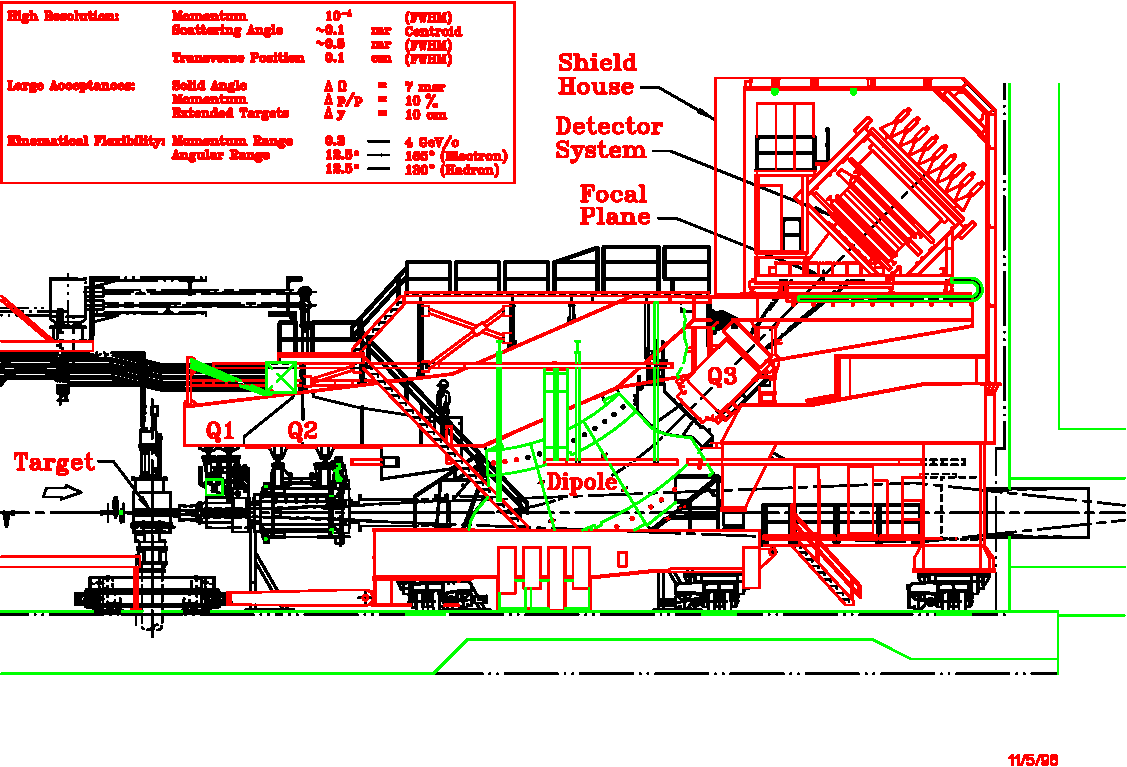
\includegraphics[angle=0,width=0.9\textwidth,clip]{figure0101_r}
\caption[Spectrometers: Elevation View of Hall~A HRS]{A side view of the Hall~A
HRS spectrometer.}  
\label{fig:hrs_ev}
\end{center}
\end{figure}
 
\begin{figure}[tbp]
\begin{center}
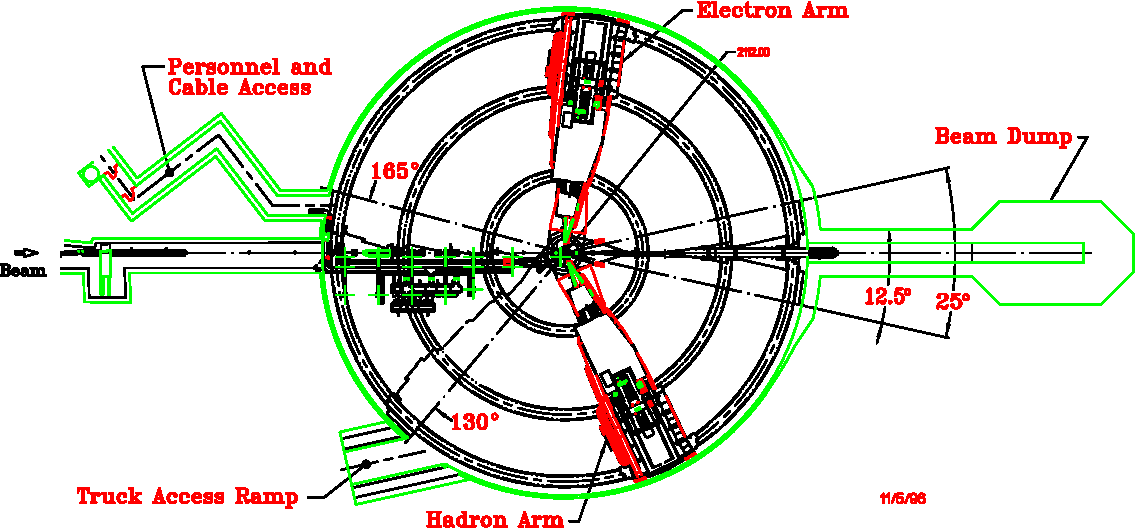
\includegraphics[angle=0,width=0.9\textwidth,clip]{figure0102_r}
\caption[Spectrometers: Plan View of Hall~A]{A bird's eye view of the Hall~A
end-station at TJNAF.}  
\label{fig:hrs_pv}
\end{center}
\end{figure}


A layout of the 4 GeV/c High Resolution Electron Spectrometer is shown 
on Figures~\ref{fig:hrs_pv} and \ref{fig:hrs_ev}.
Its main design characteristics are 
given in the attached table.  The spectrometer has a vertical bending 
plane and 45$^{\circ}$ bending angle.  The QQDQ design includes four 
independent superconducting magnets, three current-dominated 
cos2$\theta $ quadrupoles and one iron-dominated dipole with 
superconducting racetrack coils.  The second and third quadrupoles of 
each spectrometer have sufficiently similar field requirements that they 
are of identical design and construction.  The overall optical length, 
from target to focal plane, is 23.4 m.  Optically, the HRHS 
is essentially identical to HRES. In fact the two spectrometers can be used 
interchangeably to detect either positively or negatively charged particles 
as needed by any particular experiment. They are now commonly refered to 
as ``The Left Arm'' and ``The Right Arms'' rather than ``Hadron'' and ``Electron'' 

The support structure includes all system elements which bear the weight 
of the various spectrometer components and preserve their spatial 
relationship as required for 45$^{\circ}$ vertical bending optics.

The alignment and positioning system includes all the elements which 
measure and adjust the spatial relationship.  The support structure 
consists of the fabricated steel components which support the magnets, 
detector, shield house and associated equipment.  It is composed of the 
box beam, which supports the outer elements in fixed relative position 
atop the dipole; the dipole support bracket, upon which the dipole rests on 
the jacks; the cradle, upon which the dipole rests through the vertical 
positioning system, VPS; and a portion of the shield house load through 
the inboard legs of the gantry; the gantry, which supports the shield 
house and the magnet power supplies; and the bogies, which support the 
cradle-gantry assembly and roll on the floor plates and provide the 
driving power to move the two spectrometer arms.

The detector package (described in detail in Chapter \ref{chap:hrs-det})
is supported on the box beam and is surrounded by 
the shield house.  It must perform two functions, tracking and particle 
identification, PID.  The most important capability of focusing 
spectrometers is measuring precisely the momenta and entrance 
orientations of the tracks.  Momentum resolution of 10$^{-4}$ is 
obtainable, consistent with the resolution of the incident beam.

The actual configuration of the detector package varies from experiment to
experiment. The description given here is only an example of what is possible.
}

\infolevone{
A particle traversing the detector stack 
(Figure~\ref{fig:hrs_electron_det}) encounters two sets of horizontally
mounted, vertical drift wire chambers (x,y) with two planes of 368
wires in each chamber. The track resolution is $\sim$ 100 $\mu$m.  
From the chamber information both 
positions and angles in the dispersive and transverse directions can be 
determined.  The information from these chambers is the principal input 
of the tracking algorithms.

The chambers are followed by a scintillator hodoscope plane designated S1. 
This plastic scintillator array provides the timing reference for 
the drift chambers, and is also used in trigger formation and in combination 
with a second hodoscope pair it can provide time of flight particle 
identification.  These scintillators can also be used to perform crude 
tracking.

The next element encountered by a particle is a gas threshold \Cherenkov{} 
detector.  This is used for particle identification.  This gas threshold \Cherenkov{} detector can be swapped 
against an Aerogel detector, with a similar function.

The second hodoscope plane, S2, is located directly behind the 
gas \Cherenkov{}.  Its function is essentially the same as that of S1.  
In the hadron spectrometer an option exists to have this hodoscope 
pair be preceded by a third chamber, to improve tracking.
 Each of the two spectrometers 
have gas and Aerogel \Cherenkov{} detectors which can be used
 when they are in electron detection mode.

The final elements in the detector stack on HRSE are 
the pre-shower and the total-absorber lead glass shower 
calorimeter.  This is used for energy determination and PID.

\begin{figure}[tbp]
\begin{center}
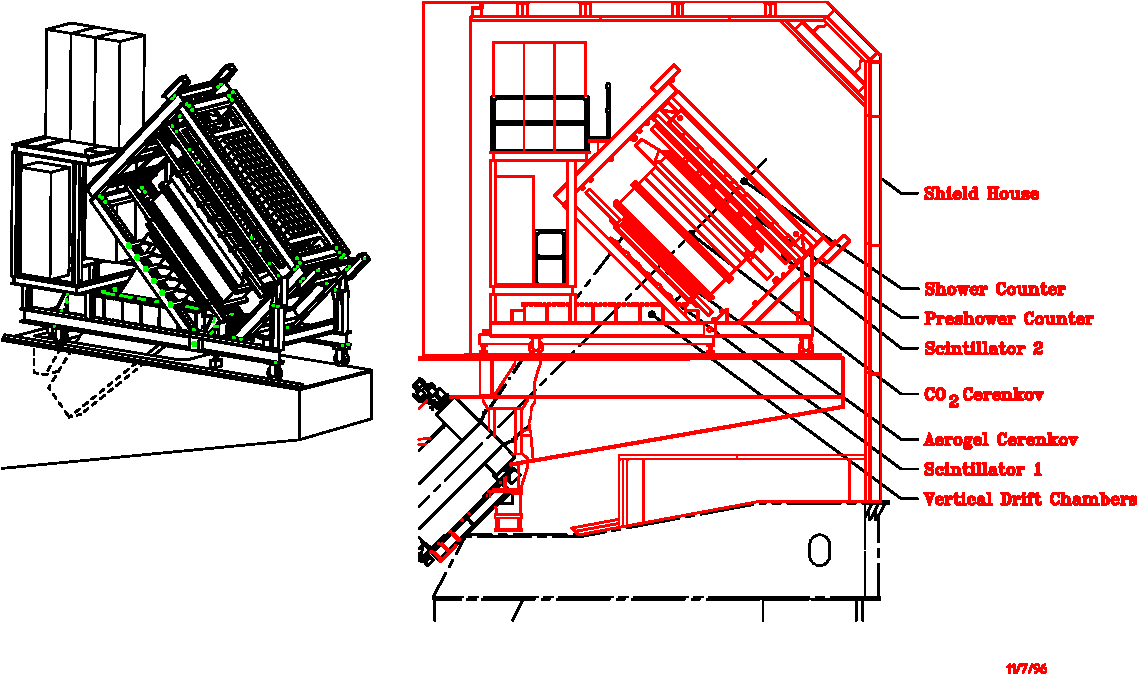
\includegraphics[angle=0,width=\textwidth,clip]{figure0103_r}
{\linespread{1.}
\caption[Spectrometers: Electron Arm Detectors]{The electron spectrometer detector stack.}
\label{fig:hrs_electron_det}}
\end{center}
\end{figure}

\begin{figure}[tbp]
\begin{center}
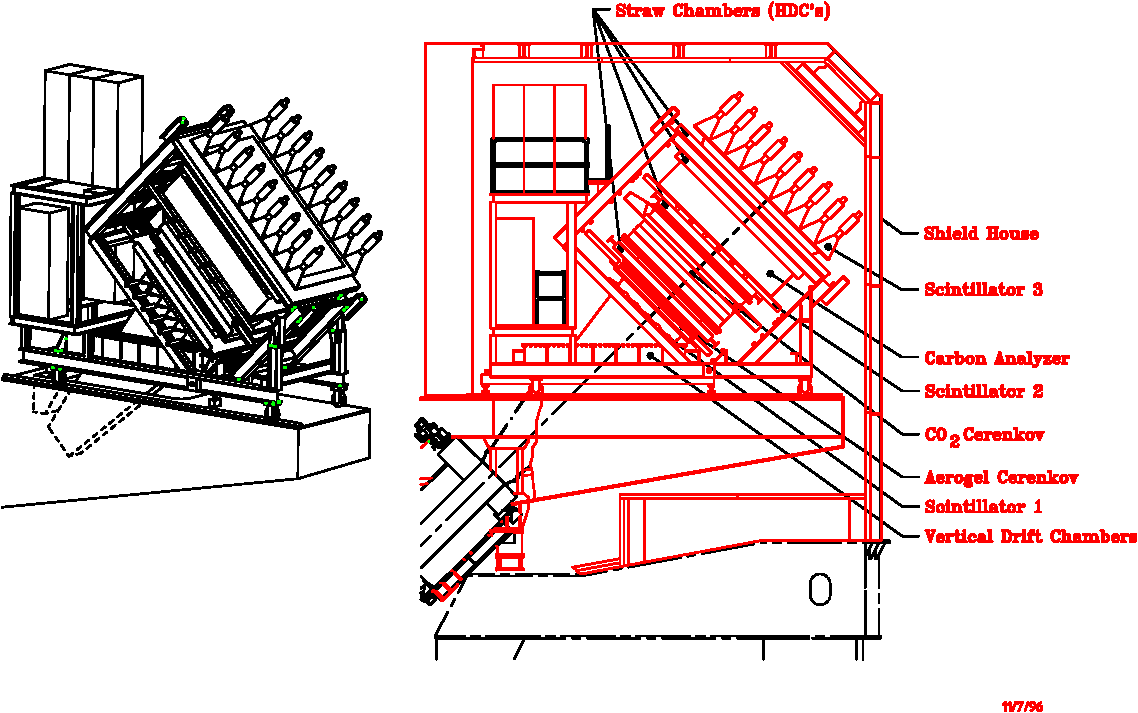
\includegraphics[angle=0,width=\textwidth,clip]{figure0104_r}
{\linespread{1.}
\caption[Spectrometers: Hadron Arm Detectors]{The hadron spectrometer detector stack.}
\label{fig:hrs_hadron_det}}
\end{center}
\end{figure}


The hadron detector is shown schematically in 
Figure~\ref{fig:hrs_hadron_det}.  It consists 
of two sets of (x,y) vertical drift wire chambers identical to those of the 
electron arm.  The remaining part of the detection system is used to 
define the level 1 trigger, as well as for particle identification and 
timing.  It consists of two minimally segmented planes of 
scintillation counters equipped with photomultipliers at both ends, and 
it includes \Cherenkov{} counters (gas CO$_2$ and Aerogel).

In addition, a proton polarimeter is installed in the back of the 
detector package to measure the polarization of the proton using a 
segmented carbon analyzer up to 60 cm in thickness to allow measurements 
over a wide range of proton energies.  A pair of front and a pair of 
rear straw tube wire chambers determine the incident and 
scattered angles, respectively.  The 
polarimeter detectors are dimensioned to accept a 20$^{\circ}$ cone of 
scattered protons.

Several support systems are necessary in addition to the basic 
components mentioned above.  They include gas supply systems for the 
wire chambers, high voltage supplies, readout electronics, a second 
level trigger, software for data analysis and testing, and a remotely 
controllable mechanical system.

For each spectrometer, all detectors are mounted on a 
single rigid support frame along with their associated electronics.  The trigger electronics are located on the support frame, next to the detectors.

To reduce the resolution degrading effects of multiple scattering, the 
entire interior of the spectrometer from the collimator box to the detector hut 
is a vacuum vessel.  The ends of this evacuated volume are capped by 
relatively thin vacuum windows.
}

\begin{safetyen}{0}{0}
\section{High Resolution Spectrometers}
\label{sec:hrs-safety}
\end{safetyen}

The principle concern with the spectrometers is that they are large, 
and have associated vacuum, hydraulic, cryogenic and magnet systems all of 
which can be potentially dangerous.

The bogies which move the massive 1200 ton spectrometers must be 
carefully operated.  Inspection of the floor and wheels to ensure there is no 
debris which the wheels could ride over is mandatory.  Similarly 
personnel need to be aware that the spectrometers are moving so that no one 
inadvertently gets trapped.

The vacuum systems associated with the spectrometers are essentially 
pressure vessels (see Chapter \ref{chap:vacuum} for more details).
Care should be exercised so as not to puncture the 
windows.

The magnets themselves are installed inside cryostats.  These vessels 
are exposed to high pressures and are therefore equipped with safety 
relief valves and burst discs.

The hydraulic system originally intended to operate the vertical positioning system (VPS) 
and the horizontal positioning system (HPS) has effectively been dismantled, after problems were encountered during the initial attempted operation of the system.

The cryogenic system operates at elevated pressure at 4K.  One must 
guard against cold burns and take the normal precautions with pressure 
vessels when operating this system.  Only authorized personnel are permitted to install 
and take out U tubes.

The magnets have a great deal of stored energy as they are large 
inductors. Always make sure people are clear of them and that
the dump resistor is attached to the magnet.

There are several major safety concerns with regards to the detectors, 
namely 1) flammable gas located in the VDC, 2) ODH hazard due to 
CO$_2$ in the \Cherenkov{} counter, 3) high voltage due to the photo 
multipliers on the various detectors and 4) a thin vacuum window 
separating the detector array from the vacuum system in the 
spectrometers.

\infolevltone{
\begin{safetyen}{5}{10}
For more information consult the full OSP manual~\cite{HallAosp}.
\end{safetyen}
} %infolev

\begin{safetyen}{10}{15}
\subsection{Authorized Personnel}
\end{safetyen}

In the event that problems arise during 
operation of the magnets, qualified personnel should be notified
(see Table \ref{tab:hrs:personnel}).  
This includes any prolonged or serious problem with the source of magnet 
cryogens (the ESR).  On weekends and after hours there will be a 
designated individual on call for magnet services.  Any member of the 
Hall A technical staff is qualified to deal with unusual magnet 
situations but in the event of serious problems the technician on
call should be contacted.

\begin{namestab}{tab:hrs:personnel}{HRS: authorized personnel}{%
      HRS: authorized personnel. ''W.B'' stands for the white board 
      in the counting house.}
   \TechonCall{\em Contact}
   \EdFolts{}
   \JackSegal{}
   \HeidiFansler{}
   \JessieButler{}
   \AndrewLumanog{}
   \JasonGlorioso{}
   \MahlonLong{}
\end{namestab}

\infolevone{
\section{The Magnets of HRS}

Each HRS is composed of three superconducting quadrupole magnets, Q1, Q2, 
and Q3, and one superconducting dipole magnet.  The large quadrupoles were 
manufactured for JLab by SIEMENS, the small quadrupole by SACLAY, while 
the dipole was built for JLab by WANG NMR.  The quadrupole magnets are 
referred to as Q1, Q2, and Q3, where a particle first traverses Q1, then 
Q2 and the dipole magnet and finally traverses Q3.

The magnet system is followed by a large steel and concrete detector 
hut, in which all detector elements reside.  Most of the 
detector elements have been built by universities involved in the Hall A 
physics program.

The HRS magnet system is the cornerstone of the Hall A activities.  
Many of the experiments approved in Hall A center on physics at high 
resolution and other short-range phenomena, and rely on a spectrometer 
able to momentum analyze charged particles up to very high momenta.  The 
design value for the maximum momentum accessible to the HRS magnet 
system is 4 GeV/c.
}

\subsection{Magnets and Power Supplies}

\infolevone{
The HRS magnet's are all superconducting and hence their coils must be 
maintained at cryogenic temperatures during operations.  The LHe 
required by the magnets is supplied by the End Station Refrigerator, ESR.

All the HRS magnets cryogenic services are supplied through the overhead 
cryogenic lines.  The distribution network begins at the distribution 
box over the pivot.  This box is connected to the rest of the network 
via the flexible transfer lines over the pivot.  The network is adjacent 
to the upstairs catwalk of the HRS.

Cryogenic information about each magnet is available on the control 
screens in the counting house, one for each magnet.  Normally during run 
periods the control screens are sent upstairs to the Hall A counting 
house and information on all the HRS magnets is available on the HRS 
control screen located in the center of the main console.  The control 
of all magnets is described in a following Section.

The power supplies for the magnets are located on the gantry balcony 
adjacent to the magnets.  The supplies are all cooled with low conductivity water (LCW).
}

\begin{safetyen}{10}{15}

Under no 
circumstances should any panel of any magnet power supply be opened by someone 
other than authorized personnel.  There are also 
signs posted listing the dangers of high magnetic fields.
\end{safetyen}

\infolevone{
A control interface for the power supplies is available through the 
HRS control screen in the Hall A counting house.
}

\infolevone{
\subsection{Quadrupole Magnets}

The quadrupoles provide some of the 
focusing properties of the spectrometer and to a large extent 
its acceptance.  Operating limits imposed on the 
quads are as follows: 1850A for Q2 and Q3 and 3250A 
for Q1.

All three quadrupoles for the HRS spectrometer are warm iron 
superconducting magnets.  The soft iron around the superconducting coil 
enhances the field at the coil center and reduces stray fields.  The 
basic parameters for the first quadrupole, Q1, are an effective length of about 
0.9 $m$, useful aperture of 0.3 $m$ and a field gradient of 9.5 
T/m.  To achieve the lowest possible angle setting of the HRS 
spectrometer (with respect to the beam line) the incident electron beam passes through
a notch in the outer yoke of Q1 when the spectrometer is at
its smallest angle of 12.5$^\circ$ . The 
other two quadrupoles, Q2 and Q3, are essentially identical with an 
effective (magnetic) length of about 1.8 meter, a useful aperture of 
0.6 $m$ and a field gradient of 3.5 T/m.
}

\infolevthree{
The maximum operating currents (assuming a 4 GeV/c momentum particle) 
for the quadrupoles are about 3000 A, 1700 A, and 1600 A, for Q1, Q2, and 
Q3, respectively.  This will render pole field values 
of 1.2, 1.0, and 1.0 T, respectively.  The energy stored in the 
quadrupole fields is sufficient to cause an unrecoverable quench if all 
the energy stored is dumped into the magnets.  Therefore a quench 
protection circuit is incorporated.  However, a quench can only happen 
if the cryomagnets have a helium level below the coil 60\% during operation.

The operating current to the Q1 quadrupole coils is provided by Danfysik 
System 8000 power supplies, which can operate up to 3500 A current and 5 
V.  The power supplies will be cooled with a combined maximum 
water flow of 45 liters per minute.

In addition to the main quadrupole windings, all quadrupoles have 
multipole windings.  To further optimize focusing properties of the HRS 
magnet system, it was intended to operate including some of these multipole 
trim coils in order to reduce higher order aberrations.
The operating current for these multipole corrections would be 
small, only (the multipole corrections are typically less than 2\% of 
the main quadrupole field), of order 50 A. Since the sextupoles were inadvertently 
installed rotated 90 $^\circ$ from their correct
orientation, these trim coils are now considered useless 
and there are at present no plans to use them.

\subsection{Cryogenic Procedures}

The cryogenics control is handled by the JLab Cryogenics Group.  The cryo control coordinator 
can be reached at the CHL (x7405) or by calling the MCC.

\subsection{First Time Startup Check List.}  

See attached check lists for all quadrupole and dipole magnets
 (Tables~\ref{tab:dip_check}, \ref{tab:q1_check}, and \ref{tab:q23_check}).
} %infolev

\infolevone{
\subsection{Dipole Magnet}

The dipole, by virtue of its field index, provides both
dispersion and focusing.  The present operations envelope 
states that the supply for the left HRS dipole may not be
operated at a current above 1800 A (4.4 GeV/c). The supply for the right HRS
dipole may not be operated above 1200 A (3.2 GeV/c), due to complications
caused by an internal short. 

The dipole for the HRS spectrometer is a superconducting, cryostable 
magnet.  Its basic parameters are an effective length of about 6.6 $m$, a 
bend radius of 8.4 $m$, and a gap width of 25 $cm$.  It is configured to 
achieve a 45 degree bending angle for 4 GeV/c momentum particles at a 
central field excitation of 1.6 T.  For the HRS dipole to reach 1.6 T 
an operating current of about 1500 A is required.
} %infolev

\infolevthree{
The dipole has been designed to achieve cryostability up to a field of 2 
T, and this property has been extensively tested up to a field of 1.6 T. 
 The cryostable coils are equipped with an energy removal circuit to 
cover the possibility of an unrecoverable quench.  However, this can 
only happen if the helium level drops below the coil during operation.  
The current to the coils will be provided by a Dynapower Corporation power 
supply, which can operate up to 2000 A and 10 V.  This 
power supply is located on the gantry beside the dipole, and will be 
cooled with a maximum water flow of 35 liters per minute.
The total water flow needed to cool the 4 power 
supplies for the HRS magnet system (dipole and quadrupoles) amounts to 
80 liters per minute, with a supply pressure of cooling water for Hall A 
of 100 psi.
} %infolev

\infolevtwo{
\section{Operation of the HRS Magnets}

\subsection{Introduction}

This is an abbreviated operating manual for 
the HRS superconducting magnets specifically designed for Hall A 
experimenters.  It provides instructions for setting currents, invoking 
NMR field regulation and general system monitoring.  Curious readers are 
directed to the references for more in-depth operating instructions and 
other technical manuals. Copies of the following supporting
documents are available in the Hall A Control Room and through the Hall A webpage
(see Table~\ref{tab:hrs-mag-manuals}).

\begin{table}[htp]
\begin{center}
\begin{tabular}{|l|l|}
\hline
References & \\
\hline 
WANG NMR Dipole & User Manual \\
Dynapower & Instruction Manual \\
Appendix & NMR Tesla meter \\
Appendix & NMR Field Regulation \\
Siemens/Fug & Q2/Q3 Magnet Instrumentation and Power Supplies \\
Saclay/Danfysik & Q1 Power Supply Manual \\
TOSP & HRS Dipole \\
TOSP & HRS Quadrupole Q1 \\
TOSP & HRS Quadrupole Q2, Q3 \\
HRS & SC Dipole Magnet Safety Review Vol. 2 \\
HRS & SC Quad Safety Review Vol. 1 \\ \hline
\end{tabular}
\end{center}
\caption[HRS Magnets: extra manuals]{HRS Magnets: extra manuals available in 
     Hall A Control Room.}
\label{tab:hrs-mag-manuals}
\end{table}

\subsection{Simple HRS Setting (Autopilot Mode)}
\label{sec:hrs-mag-set} 

 The magnets are controlled remotely using EPICS~\cite{EPICSwww} and
 EDM~\cite{EDMwww} GUI, provided that everything is working and power 
 supplies are turned on and ready to go.
 The appropriate interface runs
 on the computer \mycomp{hacsbc2} (see Section \ref{sec:contr-ha-menu}).
 On the ``Hall A General Tools'' control screen, in the upper left, there is 
 a rectangular box for each spectrometer (see Figure~\ref{fig:hrs_mag_cntrl}). 
\begin{figure}
\begin{center}
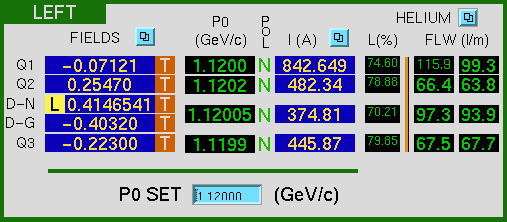
\includegraphics[angle=0,width=0.8\textwidth]{medm_halla_tools_1_cut1}
{\linespread{1.}
\caption[HRS: Magnets control]{A part of ``Hall A General Tools'' screen, 
        used for HRS (left) magnets control.}
\label{fig:hrs_mag_cntrl}}
\end{center}
\end{figure}

This box displays a brief summary of the status of the spectrometer
magnets and their cryogenic systems. The blue fields (with white
numbers) give readbacks of the magnetic fields and currents in each
magnet. The black fields also give readbacks, however in this case if
the text appears green those parameters are OK while if they are red
then that parameter is out of tolerance and may indicate a fault
condition. For example if the helium level goes below a certain point
the magnet will be automatically turned off.  In some cases it may be
desirable to monitor certain critical quantities on a strip chart
(e.g. magnet settings). A strip chart tool is available for this
purpose from the bottom of the ''EOS Menu'' button in the ''MyMenu'' window.

{\bf To set the spectrometers} for a given value of central momentum
(P0) type the desired P0 value into the light blue P0 SET box and hit
return. The magnets will be automatically 
set to the correct
values. All green numbers in the P0 column indicates that the desired
field or current settings have been reached. 

{\bf Caution:} Regarding the
dipoles, in general it's a bad idea to assume that at the first
instant that the P0 display turns green that the desired field has
been reached and you can start taking data. Stable field is in general
not achieved for from 15 to 30 minutes after reaching the nominal
desired field. This settling time depends on the magnet (the right dipole is
slower than the left dipole) and the magnitude of the field change (small
changes settle faster than big changes). Experimenters are advised to
observe both the field reading and current reading on the magnet in
question and verify that things are stable to their satisfaction
before proceeding.
 
\subsection{Powering Up Dipole Magnets:}

Use these instructions to recover from loss of a magnet due to a fault
(e.g. He level or lead flow fault). The order of actions matters. \\
(Contact Tech-On-Call if anything behaves funny or things don't
respond as expected. Sometimes after a trip an access to the Hall is
required to reset things).

\begin{list}{\arabic{enumi}.~}{\usecounter{enumi}\setlength{\itemsep}{-0.15cm}}
   \item Wait for Iout=0 (you can't and don't want to do anything while the magnet is in emergency fast dump mode.)
   \item While waiting, make a log entry re the fault. Give details such as time, coincident activities, and nature of the fault.
   \item Make sure the fault is cleared. (e.g. He level and flow rates returned to normal values and stable)
   \item In the HRS Right (Left) Dipole Systems' control panel:
   \begin{list}{}{\setlength{\itemsep}{-0.15cm}}
      \item[(a)] Press RESET (verify that all faults are cleared in the middle column)
      \item[(b)] Press ON (Display will indicate Power Supply ON and Magnet ENGAGED)
   \end{list}
\end{list}


Power supply and magnet are ready to go. From here you can return 
to "Autopilot Mode" (see Section \ref{sec:hrs-mag-set}).

\subsection{Starting Q1 Power Supply:}

 Do this when a fault causes the power supply to shut off.
 Wait for fault to clear (watch He levels). 
\begin{list}{\arabic{enumi}.~}{\usecounter{enumi}\setlength{\itemsep}{-0.15cm}}
   \item Push POWER OFF/RESET (check all faults cleared)
   \item Select desired polarity
   \item Push POWER ON
   \item Type in Setpoint (Amps) (light blue field) or re-enter P0 in Autopilot Mode.
\end{list}

\subsection{Starting Q2/3 Power Supply:}

 Do this when a fault causes the power supply to shut off.
 Wait for cause of fault to clear (watch He levels). 
 \begin{list}{\arabic{enumi}.~}{\usecounter{enumi}\setlength{\itemsep}{-0.15cm}}
   \item Push RESET 
   \item Select desired polarity
   \item Push ON
   \item Type in Current Set (light blue field) or re-enter P0 in Autopilot Mode.
\end{list}

} %infolev

\subsection{Rotation}
%
% Thanks to John LeRose for Rotation text. 07NOV2013
%
Moving an HRS
Since each HRS weighs in excess of 1,000 tons it is very important that all safety
precautions are carefully adhered to. The good news is they move very slowly (a few degrees/min
maximum), BUT 1,000 tons moving even very slowly is hard to stop. 

Hazards include:
\begin{itemize}
\item{Knocking items over.}
\item{The wheels crushing things (including fingers and toes) on the floor in the path of the 
spectrometer}
\item{Damaging the beamline or other equipment on the floor if one goes to too small 
or too large an angle, or if it just gets pushed around inadvertantly.}
\item{Tearing out of cables etc. physically attached to the superstructure}
\end{itemize}

Hazard mitigations:
\begin{itemize}
\item{Guards on either side of the wheels prevent items from getting under them.}
\item{Large pins in the floor to stop the spectrometer rotated beyond the needed angular range.}
\item{Blinking lights on the spectrometers indicating they are in motion or that motion
is possible (controls engaged etc.)}
\item{During a running experiment the run coordinator and work coordinator should know in advance 
of any moves.  Moves at any other time must be cleared with the Hall work coordinator 
before implementation.}
\item{Careful inspection of the intended path to make sure it is clear. This is part of
the pre-run checklist performed by the technical staff prior to closing the Hall and
a remote camera allows shift worker to inspect the area.}
%
%\item{Any motion that takes a spectrometer inside 14 degrees or outside x degrees
%(x being specified in the pre-run checklist and noted on the whiteboard during a run) 
%must be supervised by a trained Hall A technician.}
\end{itemize}

\infolevone{
Remote Procedure for a shift worker:
\begin{itemize}
\item{Make sure the move is part of the approved runplan (if in doubt, check with the 
run coordinator).}
\item{Check that the pre-run checklist has been completed and note and comply with any 
possible limitations to spectrometer motion (if there is a conflict inform the Run
Coordinator and do not initiate any move until the conflict is cleared).}
\item{Visually inspect the Hall using the closed circuit TV cameras to verify that there
are no obstructions.}
\item{If people are in the Hall wait until they leave (during a Controlled Access MCC keeps
track of people in the Hall). (Maybe we could soften this to "Inform EVERYONE in the Hall of
the move".)}
\item{Activate the spectrometer motion controls (see the Wiki and below) and 
move to the desired angle.}
\item{Deactivate the controls (brakes on, power off, etc.)}
\item{Update the spectrometer position information on the Hall A Controls screen}
\item{Make a halog entry indicating you've moved the spectrometer including from what angle 
to what new angle.}
\end{itemize}

Procedure for a non-run associated move in the Hall:
\begin{itemize}
\item{Inform the work coordinator of the planned move}
\item{Perform a careful visual inspection to verify that the path is clear}
\item{Check to make sure there are no temporary connections to the spectrometer (wires etc.)
that could be damaged during the move.}
\item{Inform everyone in the Hall of the move and check with them re 3.}
\item{Activate the spectrometer motion controls (see the Wiki and below) verify 
that the warning lights are on and move to the desired angle.}
\item{Deactivate the controls (brakes on, power off, etc.).}
\end{itemize}

The full proceedure for moving the spectrometer follows and can also be found on the Hall A wiki.

On hacsbc2, click the red "tool box" icon on the linux taskbar, as above. Choose 
bogies\_SetSpec so that you can determine the angle and vernier setting for the spectrometer.
Enter the spectrometer (L or R), and the angle, and you will get two options for the floor 
mark and the vernier. Generally choose the vernier closer to zero. Center the cameras on the 
desire vernier using the Move+/Move- buttons on the Hall A General Tools screen. The TV monitors 
for these cameras are on the middle shelf, in rack CH01A05.

Choose bogies\_Left (or bogies\_Right) in the tool box to bring up the bogies control screen. 
Click PSM enable and wait a few seconds for PSM OK to read YES. 
Click DM enable and wait a few seconds for DM OK to read YES.
Make sure the velocity is set to 0 and the direction is CW or CCW as desired. Click on Brake Release 
and wait for Brakes OK to read YES.

Click on ClampRelease, set the velocity to 700. Once you see the spectrometer start to move in the 
floor angle camera - you cannot see the spectrometer move in the Hall overview camera, as it only 
moves a few degrees per minute at maximum speed. For the left arm, to move to a larger angle, the 
direction should be CCW, while for the right arm CW moves the spectrometer to larger angle. The 
direction of the spectrometer is reversed by using a negative rpm. Watch the spectrometer motion 
on the cameras. When you are getting close to the desired angle, slow down to about 300 rpm. 
To stop, click on the Clamp Release button and the Brake button. Disable DM and PSM, and disconnect 
to close the GUI. Read off the floor angle mark and vernier, and input the values into the appropriate 
fields in the Alignment section of the Hall A General Tools GUI. 
}









\newpage
\section[Field Monitoring]{Field Monitoring
\footnote{
  $CVS~revision~ $Id: nmr-1999.tex,v 1.4 2003/12/17 03:59:48 gen Exp $ $ 
}
\footnote{Authors: J.LeRose \email{lerose@jlab.org}}
}

The field-monitoring controls are available using the main 
HRS screen%
\infolevtwo{ (see Figure~\ref{fig:hrs_mag_cntrl})%
}. % infolev
The dipoles' field is measured using NMR Teslameters and
field probes.

\infolevone{ 
 
\subsection{ Dipole Field Monitoring Electron Arm}

\noindent {\bf Basic Setup}

Each spectrometer dipole magnet is equipped with a Metrolab PT 4025 
NMR Teslameter, several field probes, and multiplexers (to allow switching 
between the probes).  Details of the operation and theory of operation 
for the Teslameter can be found in its user manual, 
a copy of which is available in the the counting house.
The basic layout is shown in Figure~\ref{fig:nmrbasic}


\begin{figure}
\begin{center}
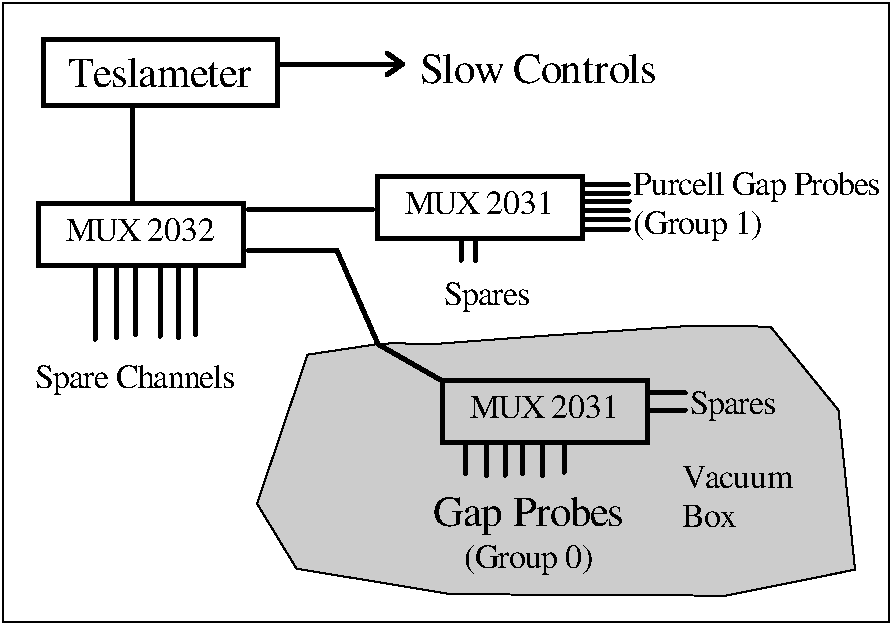
\includegraphics[angle=0,width=15cm,clip]{lerose_fig1}
{\linespread{1.}
\caption[Spectrometers: NMR System Layout]{Basic layout of NMR system}
\label{fig:nmrbasic}}
\end{center}
\end{figure}


 The "Gap Probes" (Group 0 in the controls) are located in two groups 
of three; one group on the low field side of the gap and the other on the high 
field side of the gap.  The groups of three are made up of one each of 
the manufacturer's type 3, 4 \& 5 probes, designed to cover different 
field ranges (see Table \ref{nmr_range}).  The six ``Purcell Gap Probes'' (Group 1 in 
the controls) are located in the Purcell gap of the magnet 
and consists of two each of the above types. {\em Note: Since
the fall of 1998 the multiplexer-multiplexer in both arms,
MUX 2032, has been removed and hence the ``Purcell Gap Probes'' are currently
unavailable. There are no plans to re-install this multiplexer.}

 The "Gap Probes" are equipped with coils which provide a field 
gradient that cancels out the field gradient of the magnet in the vicinity of 
the probe.  These gradient compensating coils are part of a simple circuit 
that is completely independent of the Teslameter.  The basic circuit for 
the compensating coils is shown in Figure~\ref{fig:nmrcir}


\begin{figure}
\begin{center}
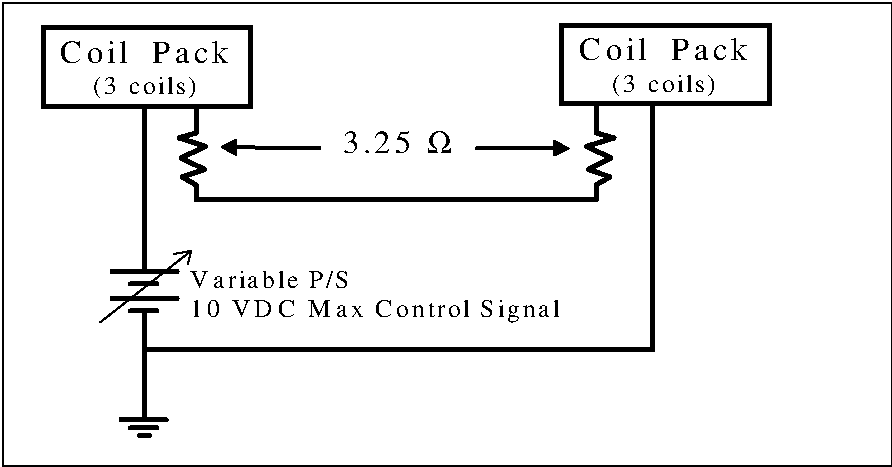
\includegraphics[angle=0,width=10cm,clip]{lerose_fig2}
{\linespread{1.}
\caption[Spectrometers: NMR Gradient Compensation]{Gradient Compensating Circuit.}
\label{fig:nmrcir}}
\end{center}
\end{figure}


%\snfig{figs/lerose_figcce.eps}{Control Voltage calibration for
%Electron Dipole }{nmrcomp4}{5in}

\begin{figure}
\begin{center}
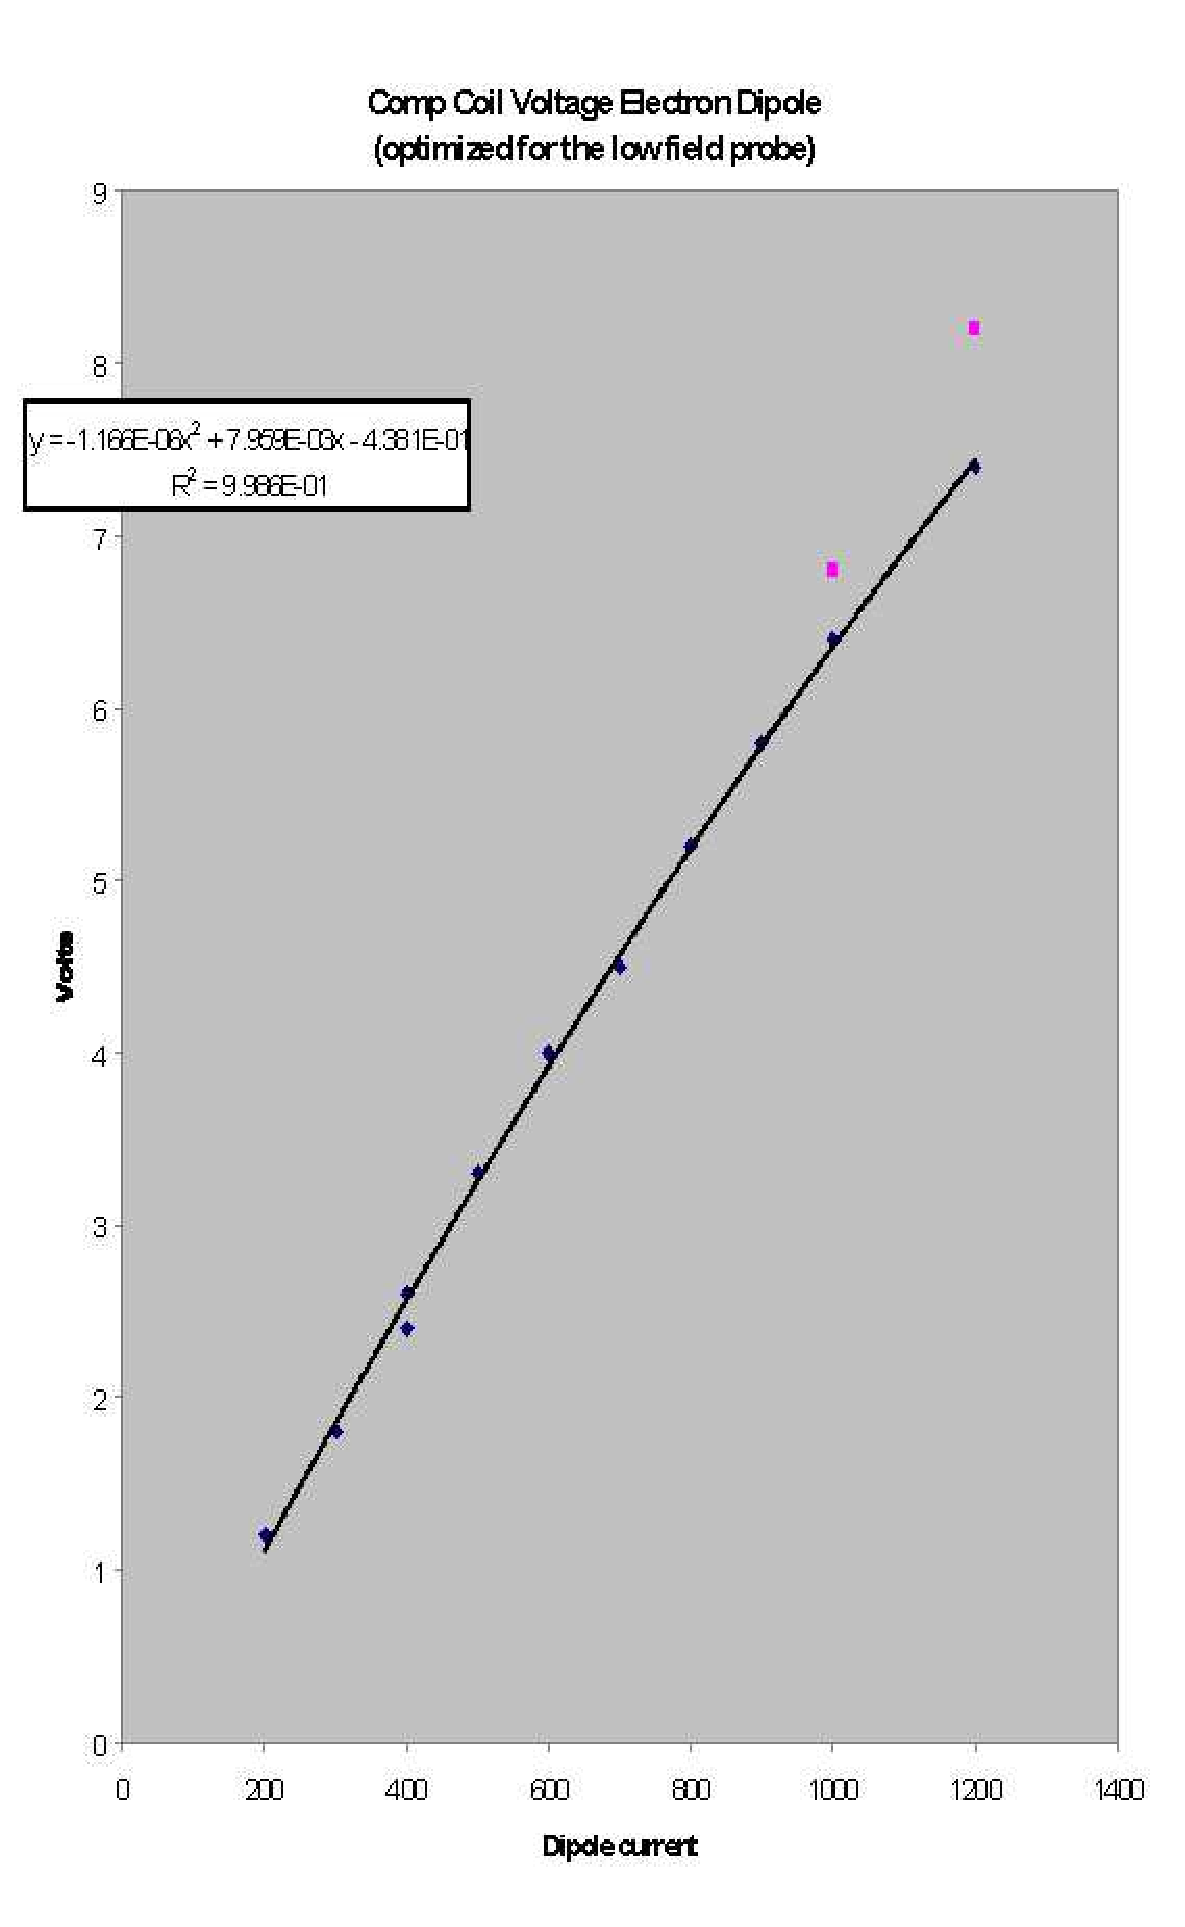
\includegraphics[angle=0,height=20cm,clip]{lerose_figcce}
{\linespread{1.}
\caption[Spectrometers: Control Voltage Calibration for Left Dipole]{Control Voltage calibration for the Left Dipole.}
\label{fig:nmrcomp4}}
\end{center}
\end{figure}

%\snfig{figs/lerose_figcch.eps}{Control Voltage calibration for
%Hadron Dipole }{nmrcomp5}{5in}
\begin{figure}
\begin{center}
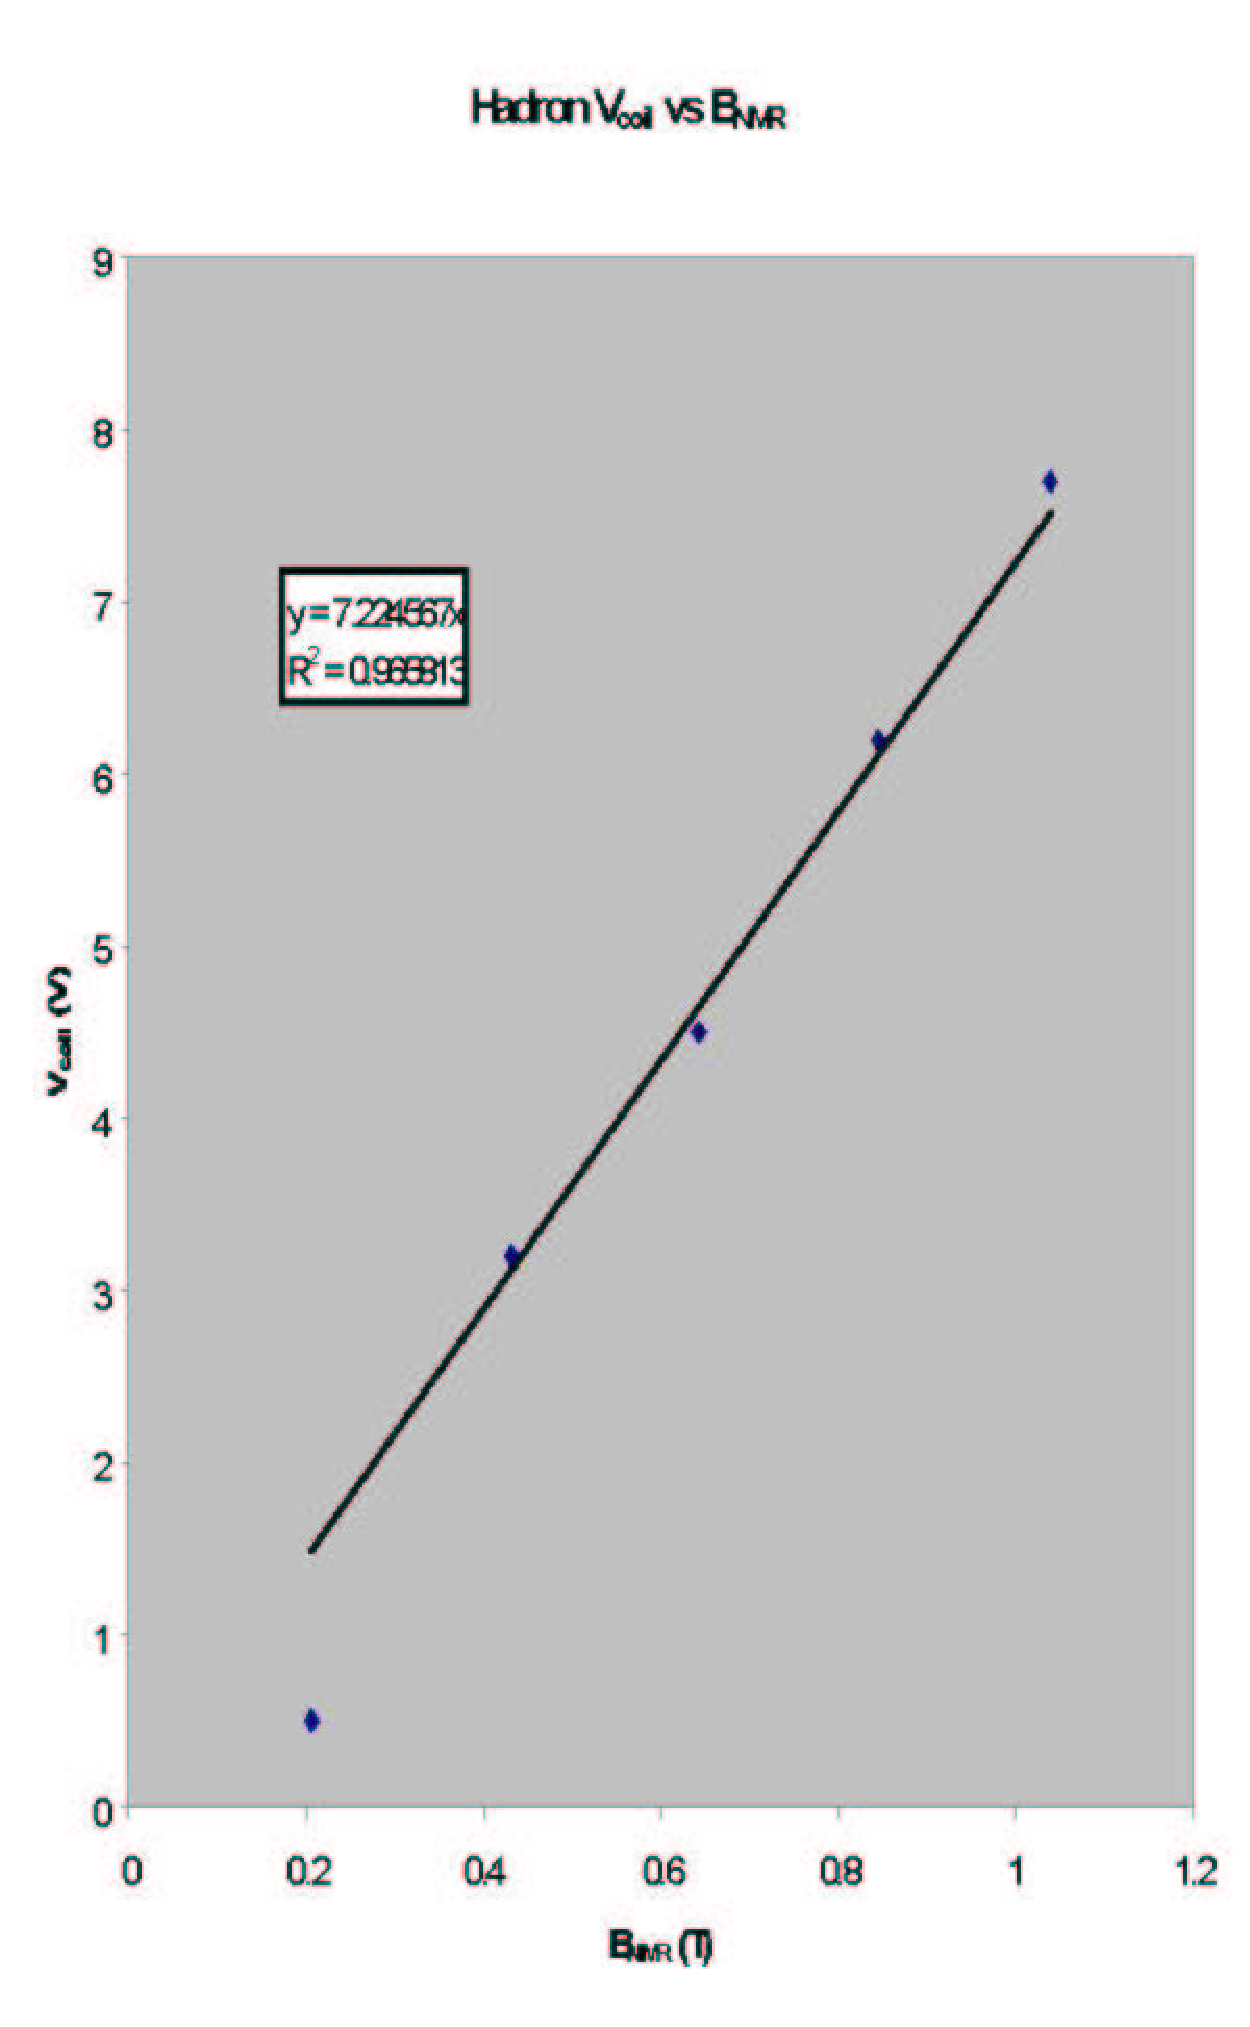
\includegraphics[angle=0,height=20cm,clip]{lerose_figcch}
{\linespread{1.}
\caption[Spectrometers: Control Voltage Calibration for Right Dipole] {Control Voltage calibration for the Right Dipole.}
\label{fig:nmrcomp5}}
\end{center}
\end{figure}

%\snfig{./figs/lerose_fig7.eps}{DAC Calibration for manual operation of NMR probes}{nmr_dac}{9in}
\begin{figure}
\begin{center}
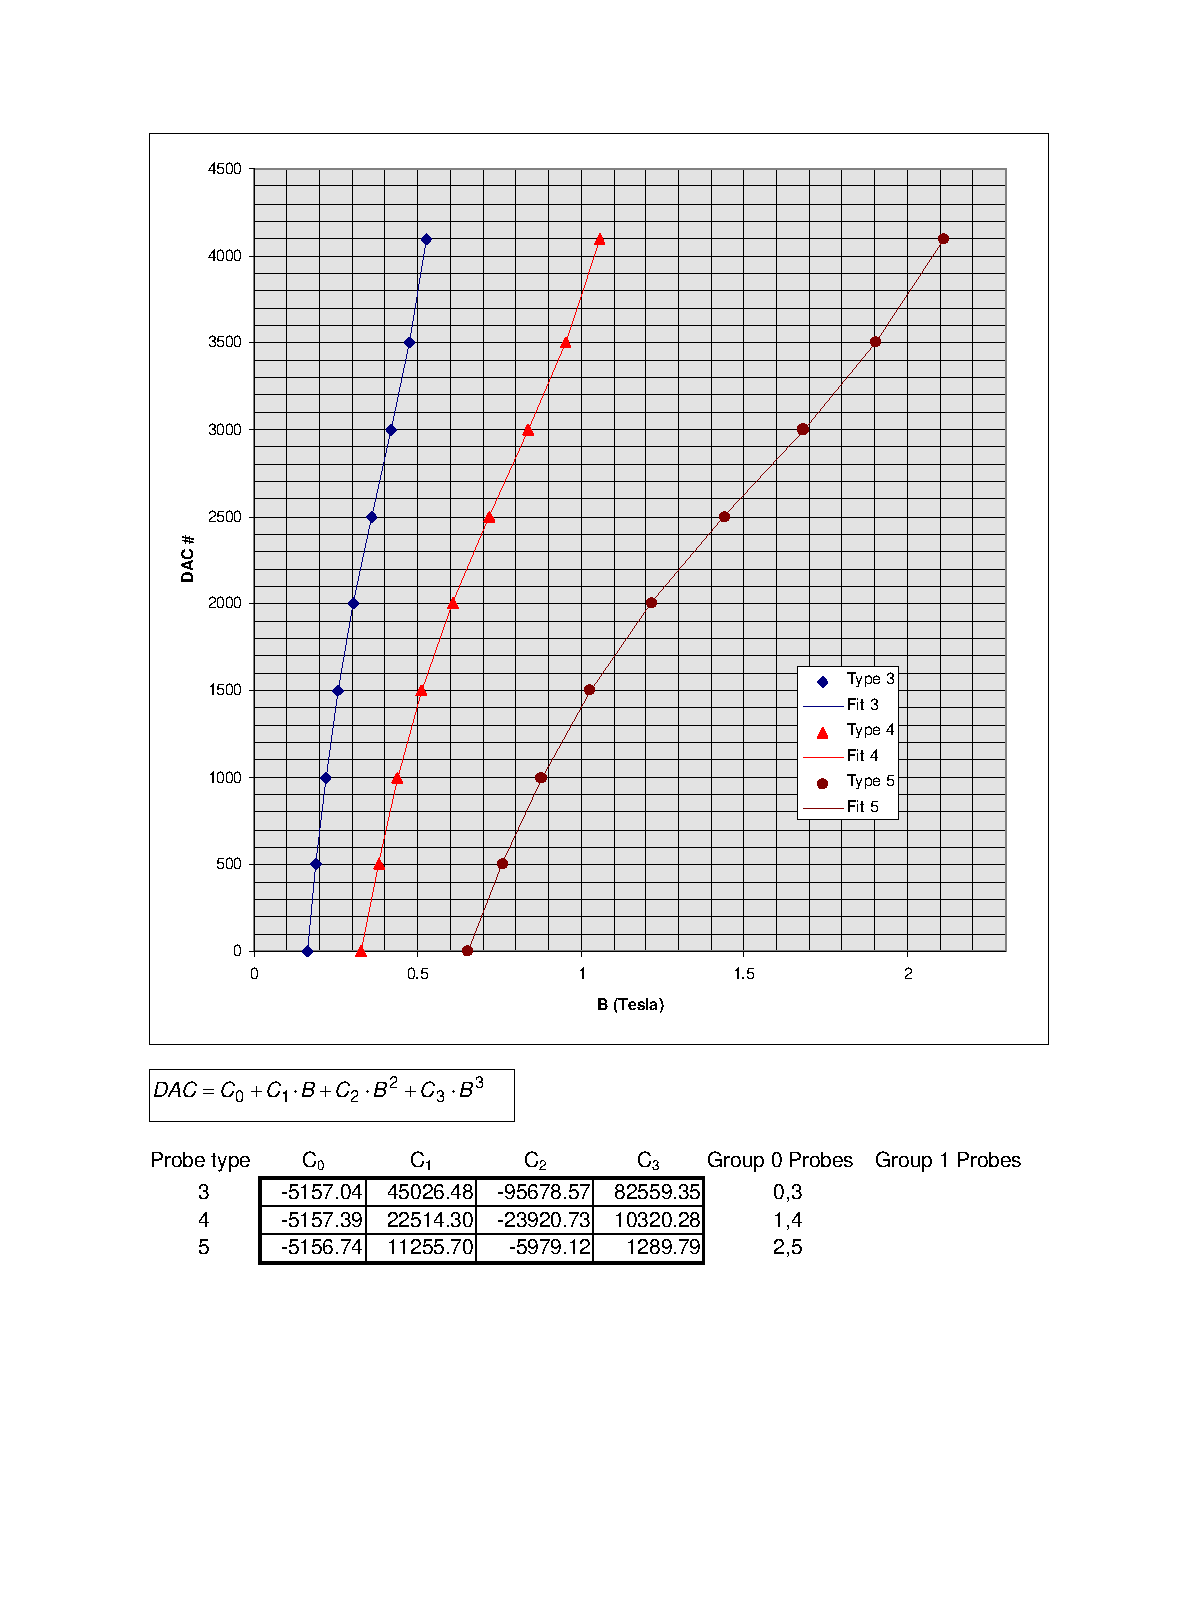
\includegraphics[angle=0,height=20cm,clip]{lerose_fig7}
{\linespread{1.}
\caption[Spectrometers: NMR Probe DAC Calibration]{DAC Calibration for manual operation of NMR probes.}
\label{fig:nmr_dac}}
\end{center}
\end{figure}

The following graphs (see Figures~\ref{fig:nmrcomp4} 
and ~\ref{fig:nmrcomp5}),can be used to determine optimum values for the 
compensating coil control voltage.  It should be noted that the setting 
of the compensating coil current is not very critical in most cases.  In 
general if you're within 10\% of the correct value everything should 
work fine.



\begin{table}
\begin{center}
\begin{tabular}{|cc|} \hline
Probe Type & Field Range (T) \\ \hline 
3 & 0.17 - 0.52 \\
4 & 0.35 - 1.05 \\
5 & 0.70 - 2.10 \\ \hline
\end{tabular}
\caption[Spectrometers: Dipole NMR Probe Field Ranges]{Dipole NMR probe field ranges}
\label{nmr_range}
\end{center}
\end{table}

} %infolev

\infolevtwo{
\subsection{NMR Operating Procedure}

When running in Autopilot mode (see: Simple Spectrometer Field Setting) the 
compensating coil voltage is set automatically and the probe appropriate for 
the field desired is selected. The gaussmeter is placed in SEARCH Mode and the 
dipole power supply software regulator is turned on. In this case the dipole current is 
adjusted to achieve the desired field. The user should just stand 
back and let it work. What follows are instructions for using
the NMR gaussmeter in situations where Autopilot doesn't work or
some special supplemental measurements are required. 

 In principle it is possible to make the field measurements using the 
SEARCH mode in the Teslameter.  In this mode you select a probe and the 
meter explores the whole field range of the probe until it finds and 
"locks" on the resonant signal indicating that it has a field 
measurement.  A ``lock" is indicated on the controls display by an ``L'' to 
the left of the field values.  This has the advantage of simplicity but in practice can 
be time consuming and doesn't always work.  The problem being, in 
situations where there is a lot of noise mixed in with the signal, the 
circuitry has problems distinguishing the signal from the noise and gets 
lost before it ever finds a lock.  The problem is exacerbated when the 
field being measured is at the high end of the probe's range.  In this 
case the search starts at the low end and keeps getting hung up on the 
noise and never gets to the field range of interest.  The solution to 
this problem is to tell the device approximately what field it's looking 
for and use the AUTO mode to find the lock.  In the procedure below that 
is what we will be doing.

In any case, for ``gap probes" (group 0) you must energize and adjust 
the gradient compensating coils for the field ranges to be measured before 
trying to make a measurement.

For studies involving 
10\% changes in the field settings the compensating coil current can be 
set once and left alone.


\noindent\underline{\bf Recommended Procedure:}(turn the {\bf SOFTWARE REGULATOR OFF} for all 
non-autopilot field measurements)\\
For group 0 probes set compensating coils appropriately (see figures).\\
Put the meter in MANUAL mode with SEARCH OFF \\
Select a probe \underline{\bf and} polarity (\underline{\bf Group 0:  
Probes 0, 1, 2 negative; Probes 3, 4, 5 positive}) \\
Type in the appropriate DAC number for the field range being measured (see below) \\
Select AUTO and wait for a lock (indicating a valid field reading) \\
Verify that you have a good lock by checking the oscilloscope for a 
clear resonant signal. \\
If you have problems see the table listing problems and possible 
solutions.

\noindent\underline{\bf Selecting DAC Number}

In selecting the DAC number to use for the field of interest use 
either the graph in Figure~\ref{fig:nmr_dac} or the polynomial at the bottom of the same figure.

\pagebreak
\noindent{\bf Problems and Solutions}\\
\begin{table}[htb]
\begin{tabular}{|p{0.4\textwidth}|p{0.55\textwidth}|}\hline
Symptom & Diagnosis and Cure \\ \hline\hline
Weird numbers on displays, controls for all magnets fouled up 
& Need to reboot.  See instructions below. \\ \hline
NMR Teslameter does not respond to commands and display shows all zeros. 
& Meter's communications are somehow hung up. Push {\bf RESET}. \\ \hline
%Will not lock & Very high noise level makes resonance hard to find. \\
%Still 
Will not lock 
& Very high noise level makes resonance hard to find. Search for the resonance manually by 
  adjusting the DAC in manual mode until you see the resonant signal.  (It helps if you know 
  what field you expect so you'll know where to look). \\ \hline
You find resonance manually but still can't get a lock 
& Check probe polarity. Try decreasing and increasing DAC number by 1. Optimize signal 
  by adjusting compensating coils. \\ \hline
Can't find resonance manually 
& Try a different probe.  Use readings from other probes to tell you where to look for 
 the resonance with the probe that's giving you trouble.  Make sure
 compensating coils are energized properly.  Make sure magnet is on. \\ \hline\hline
\end{tabular}
\caption[NMR: Problems and solutions]{NMR: Problems and solutions}
\label{tab:nmr-problems-solutions}
\end{table}

\begin{table}[ht]
\begin{center}
\begin{tabular}{|p{0.3\textwidth}|p{0.3\textwidth}|p{0.3\textwidth}|}\hline
Problems & Explanation & Action \\ \hline
NMR not locked but current is changing in the right direction 
& Normal operation for large field changes  
& Wait. (see above) \\ \hline
NMR locked but current going in the wrong direction.
& Normal operation. 
& Wait. \\ \hline
NMR locked but field not correct and current not changing 
& Field regulation is disabled or software is confused.
& Check that field regulation is enabled. Enter desired field value or one
  very near the desired value again. \\ \hline
NMR field display freezes. (Usually but not always shows  -\#.0000000)
& NMR Gaussmeter is not communicating with software.
& Push {\bf RESET}. \\ \hline
\end{tabular}
\end{center}
\caption[NMR troubleshhoting]{NMR troubleshooting
}
\label{tab:hrs_nmr_2}
\end{table}

} %infolev

\begin{safetyen}{10}{15}
\subsection{Authorized Personnel}
\end{safetyen}

The individuals shown in Table \ref{tab:nmr:personnel} are responsible for NMR operation problems.

\begin{namestab}{tab:nmr:personnel}{NMR: authorized personnel}{%
      NMR: authorized personnel.}
  \JavierGomez{\em Contact}
  \JohnLeRose{}
\end{namestab}



\newpage
\section[Collimators and Sieve Slits]{Collimators and Sieve Slits
\footnote{
  $CVS~revision~ $Id: slit.tex,v 1.5 2003/12/13 06:23:38 gen Exp $ $ 
}
\footnote{Authors: J.LeRose \email{lerose@jlab.org}}
}

Both spectrometers have front-end devices for calibrating the optical
properties of the spectrometers. These are known as the collimator boxes.
These boxes are positioned between the scattering chamber and the 
first quadrupoles (Q1). Each box is carefully aligned and rigidly attached
to the  entrance flange of the Q1 of the respective spectrometer.  The boxes are
part of the vacuum system of the spectrometer.
In the septum configuration sieve slits and collimators are installed and removed manually.

Inside each box a ladder is mounted which is guided by a linear bearing
and moved up and down by a ball screw. On this ladder 3 positions are 
available to insert collimators. Below this ladder
a special valve is mounted that can isolate the vacuum in the spectrometer
from the target system. This valve should be activated when it is moved
in front of the holes connecting the box with spectrometer and target chamber.
\infolevone{
A schematic view of the collimator box is shown in Fig.~\ref{fig:coll}.

\begin{figure}
\begin{center}
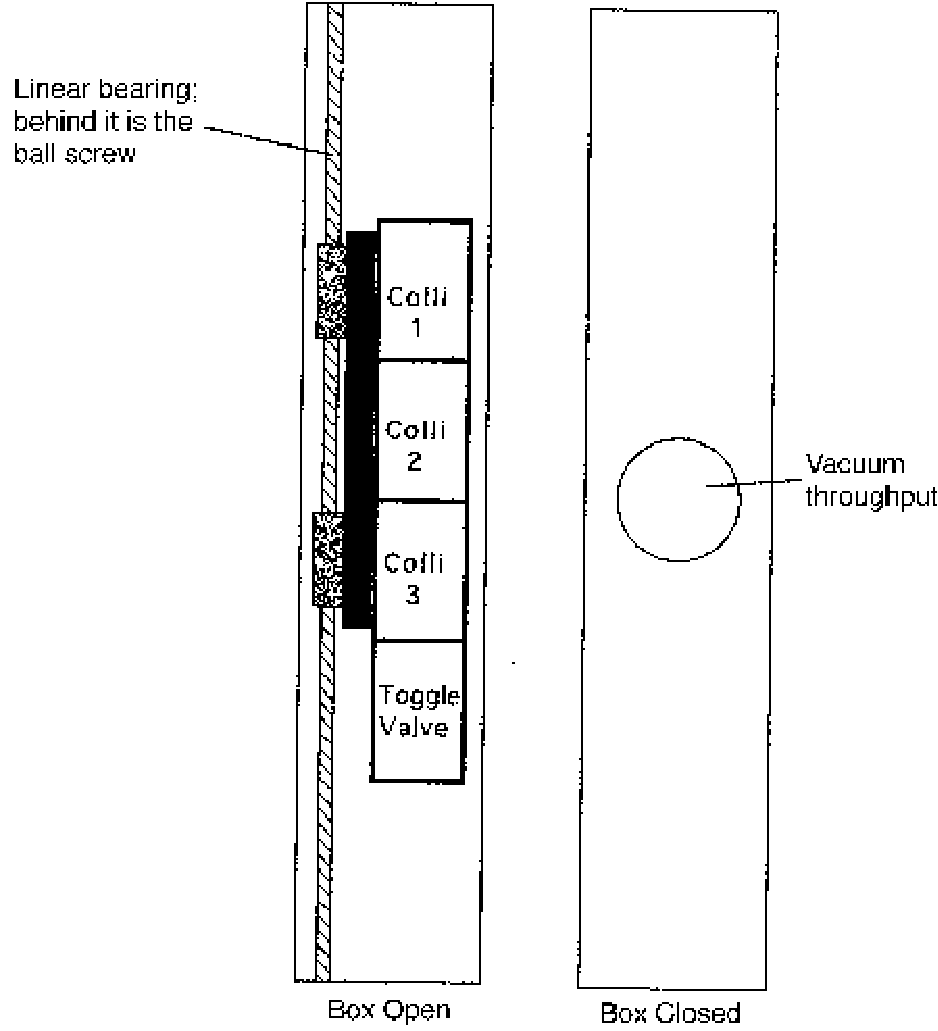
\includegraphics[angle=0,width=13cm,clip]{collimator_clip}
{\linespread{1.}
\caption[Spectrometers: Collimator Box Schematic]{Schematic layout of the collimator box.}
\label{fig:coll}}
\end{center}
\end{figure}
} %infolev

Vacuum requirement is $10^{-6}$ Torr. The material for the box is 
aluminum. It is possible to open one side of the box so that
collimators can be exchanged. The
reproducibility of collimator positions after moving
the ladder and/or after replacing a collimator is
better than 0.1 mm in horizontal and vertical direction.
The dimensions of the box are
roughly height=175 cm , width=35 cm and depth=15 cm.
The tolerance in the dimension
of the 7 msr collimator hole is $\pm0.5$ mm in each direction. 
The tolerance in the position
of each of the sieve-slit holes is $\pm0.1$ mm in each direction.

\infolevone{
\begin{figure}
\begin{center}
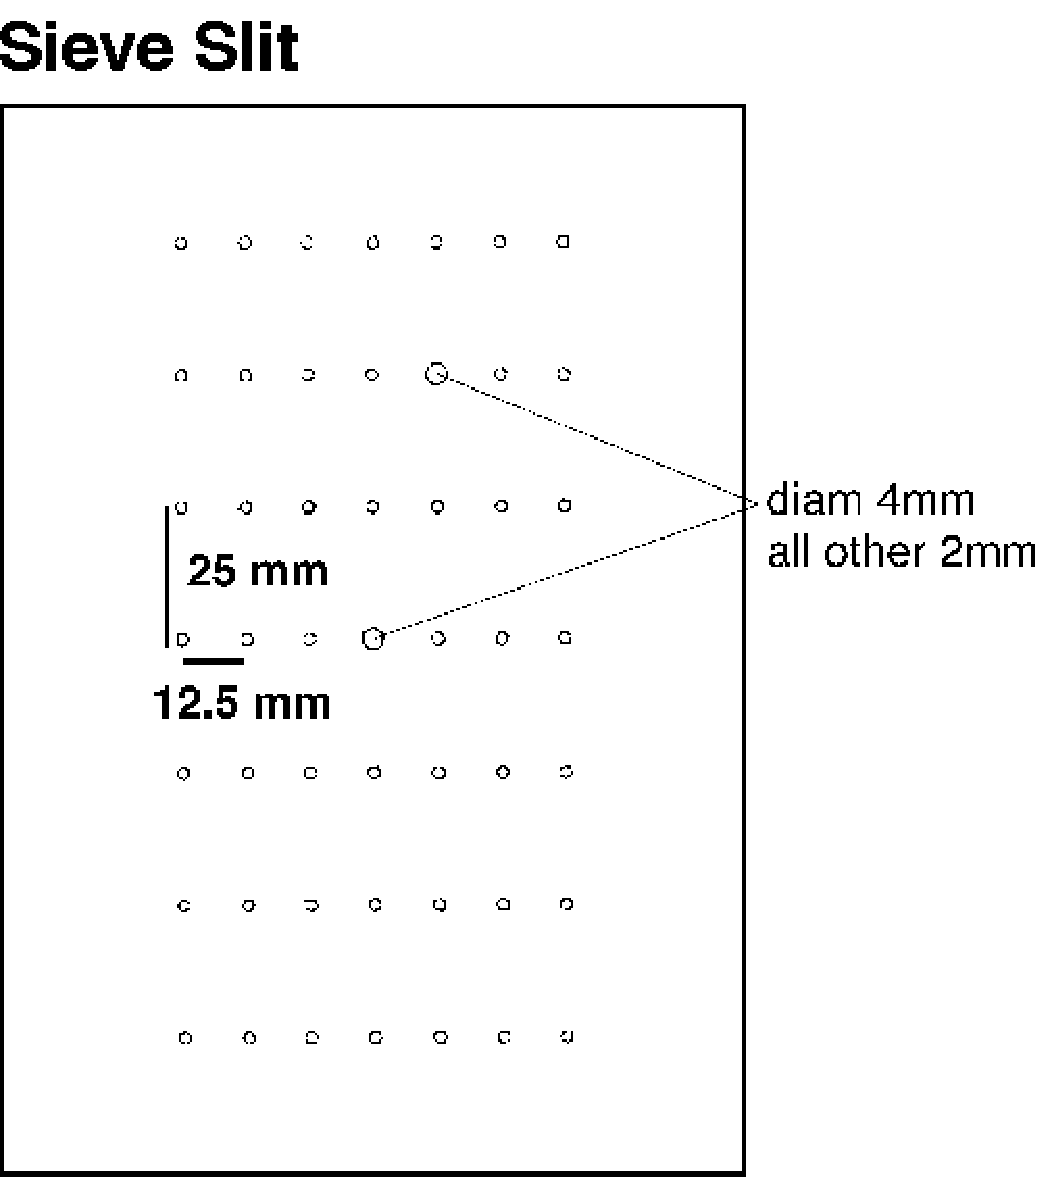
\includegraphics[angle=0,width=13cm,clip]{sieveslit}
{\linespread{1.}
\caption[Spectrometers: Sieve Slit]{Sieve slit collimator for optics calibration.}
\label{fig:sieve}}
\end{center}
\end{figure}
} %infolev
A typical sieve slit collimator 
\infolevone{(shown in Fig.~\ref{fig:sieve})
} %infolev 
consists of a plate of roughly 14 cm x 20 cm containing 49 holes
positioned in a regular 7x7 pattern. This slit is made out of 5
mm thick tungsten.
The holes have a diameter of 2 mm except for the central one and one positioned
off-diagonal which have a diameter of 4 mm. The horizontal distance between the
holes is 12.5 mm while the vertical distance is 25.0 mm.
%
%To get the latest information on the dimensions and locations of the collimators see 
%the Hall A homepage on the web%
%\htmladdnormallinkfoot{}{\url{
%http://hallaweb.jlab.org/
%}}.

To get the latest information on the dimensions and locations of the collimators see 
the Hall A homepage on the web%
\htmladdnormallinkfoot{}{\url{
http://hallaweb.jlab.org/
}}.

\begin{safetyen}{10}{15}
\subsection{Safety Assessment}

The collimator boxes form part of the vacuum system for each spectrometer. All hazards
identified in section spectrometer vacuum section applies to the collimator box as well.

In addition, safe access to the top of
the collimator boxes is needed  during manual operation of the box as outlined below.
Due to the proximity of the collimator boxes to the scattering chamber, and Q1 quadrupoles,
all necessary safety precautions with regards to vacuum windows, electrical power cables, 
cryogenic transfer lines, and high magnetic field should be taken. The same precautions also apply 
to the collimators and sieves in the septum configuration. In that case the sieve and collomators
can be considered part of the beamline. A survey and
appropriate RADCON designated proceedures must be followed when dealing with septum sieves 
and collimators.
\end{safetyen}

\infolevtwo{
\subsection{Operating Procedure}
Slit position is changed remotely from the standard Hall A control screen.
In the case of a spectrometer configuration involving the septum magnets collimators and sieves are
changed manually in the Hall.
} %infolev

\subsection{Authorized  Personnel} 

\begin{itemize} 
\item[~]E. Folts - x7857 (mechanical and vacuum systems).
\item[~]J. Gomez - x7498 (computer controls and electrical systems).
\end{itemize} 

% ===========  CVS info
% $Header: /group/halla/analysis/cvs/tex/osp/src/hrs/slit.tex,v 1.5 2003/12/13 06:23:38 gen Exp $
% $Id: slit.tex,v 1.5 2003/12/13 06:23:38 gen Exp $
% $Author: gen $
% $Date: 2003/12/13 06:23:38 $
% $Name:  $
% $Locker:  $
% $Log: slit.tex,v $
% Revision 1.5  2003/12/13 06:23:38  gen
% Septum added. Name tables. Polishing
%
% Revision 1.4  2003/12/05 06:49:07  gen
% infolevels added, polishing
%
% Revision 1.3  2003/06/06 16:13:37  gen
% Revision printout changed
%
% Revision 1.2  2003/06/05 23:30:00  gen
% Revision ID is printed in TeX
%
% Revision 1.1.1.1  2003/06/05 17:28:31  gen
% Imported from /home/gen/tex/OSP
%
%  Revision parameters to appear on the output

\newpage
\infolevtwo{
\section[Spectrometer Alignment]{Spectrometer Alignment
\footnote{
  $CVS~revision~ $Id: AlignmentOps.tex,v 1.8 2003/12/17 03:59:48 gen Exp $ $ 
}
\footnote{Authors: J.Gomez \email{gomez@jlab.org}}
}

At present, the systems implemented to determine the alignment of each spectrometer
(roll, vertical angle/pointing and horizontal angle/pointing) without the help of the
Accelerator Division Survey group are limited to roll, vertical angle and horizontal angle.
All alignment information is displayed in the ``ALIGNMENT'' mosaic of the ``Hall A
General Tools'' EDM screen%
\infolevtwo{ (see Fig.~\ref{fig:medm-hlamain-tools})}
(``EOS Menu'' $-->$ ``EDM (HLA Main)'' $-->$ ``Hall A Main Menu'' $-->$ ``Tools'').

A bi-axial inclinometer is used to determine the roll and vertical angle (also known as pitch)
of each spectrometer. These inclinometers are attached to the back of the dipoles at the power
supply platform level. The raw inclinometer measurements, in Volts,
are displayed as ``Tilt X'' and ``Tilt Y''. The inclinometer temperature is also given
(`` Tilt T''), in degree Celsius. From these values, the ``ROLL'' and ``PITCH'' values are
calculated.
Agreement between the inclinometer readings and survey measurements
are better than $\pm$ 0.1 mrad over all presently available history.

The horizontal spectrometer angle is determined from floor marks set in
place by the survey group. Floor marks have been placed every 0.5 $^\circ$ covering the useful range of
both spectrometers.
There are two concentric rings of floor marks in the hall. We will concentrate in the
inner ring which covers the angular range of both spectrometers. The outer ring is
similar.
The inner-ring floor marks are located at a distance of $\sim$10 $m$ from the target center.
A ruler attached to each spectrometer dipole runs over the floor marks and it acts as a vernier to interpolate
between marks. The location of a given floor mark on the ruler can be viewed from the Hall A Counting
House through a TV camera (labeled ``Front Camera'') .
The camera is able to move along the length of the ruler so that any
parallax effect can be eliminated. The camera motion is controlled from the ``Tools'' screen
through two push buttons (``FRONT CAMERA'' - ``MOVE +'' and ``MOVE --'').
Two fields in the ``ALIGNMENT'' mosaic
(``Flr Mrk'' and ``Vernier'') allow to input
the values read from the TV monitor. The effective spectrometer angle is then calculated and displayed
as ``Angle''. The application ``HRS Floor Marks'' calculates the floor mark and vernier value
to which the spectrometer should be set
to obtain a given angle. Spectrometer horizontal angle surveys and floor mark determinations
agree to $\pm$ 0.2 mrad.

\newpage
\begin{safetyen}{10}{15}
\subsection{Authorized  Personnel} 
\end{safetyen}
The authorized personnel is shown in table \ref{tab:align:personnel}.
\begin{namestab}{tab:align:personnel}{HRS alignment: authorized personnel}{%
      HRS alignment: authorized personnel.}
  \JessieButler{\em Contact}
\end{namestab}

} %infolev


% ===========  CVS info
% $Header: /group/halla/analysis/cvs/tex/osp/src/hrs/all.tex,v 1.3 2003/06/06 15:44:08 gen Exp $
% $Id: all.tex,v 1.3 2003/06/06 15:44:08 gen Exp $
% $Author: gen $
% $Date: 2003/06/06 15:44:08 $
% $Name:  $
% $Locker:  $
% $Log: all.tex,v $
% Revision 1.3  2003/06/06 15:44:08  gen
% Revision printout changed
%
% Revision 1.2  2003/06/05 23:30:00  gen
% Revision ID is printed in TeX
%
% Revision 1.1.1.1  2003/06/05 17:28:31  gen
% Imported from /home/gen/tex/OSP
%
%  Revision parameters to appear on the output

\graphicspath{{figs}}
% Compton Polarimeter
\infolevone{\chapter[Compton Polarimeter]{Compton Polarimeter}
\label{sec:compton}
\footnote{Author: S.Nanda \email{nanda@jlab.org}}
}
\infoleveqnull{\section{Compton Polarimeter}}

\newcommand{\dis}{\displaystyle}
\newcommand{\nn}{\nonumber}
\newcommand{\aexp}{A_{exp}}
\newcommand{\araw}{A_{raw}}
\newcommand{\ath}{A_{{th}}}
\newcommand{\ac}{A_{{c}}}
\newcommand{\af}{A_{{F}}}
\newcommand{\pe}{P_{{e}}}
\newcommand{\pg}{P_{\gamma}}
\newcommand{\np}{N^{+}}
\newcommand{\nm}{N^{-}}
\newcommand{\kp}{k^{\prime}}
\newcommand{\krs}{k^{\prime s}_{r}}
\newcommand{\sigrs}{\sigma^{s}_{r}}
\newcommand{\sigc}{\sigma_{c}}
\newcommand{\kmax}{k^{\prime}_{max}}
\newcommand{\wer}{\omega_R}
\newcommand{\wel}{\omega_L}

\infolevone{
\section {Introduction}
\label{sec:compton_introduction}
In order to measure the longitudinal polarization of the 3-6 GeV high intensity TJNAF electron beam, a
Compton Polarimeter was built by CEA Saclay,
LPC Clermont-Ferrand,
and
Jefferson Laboratory.
The Compton polarimeter has been running since february 1999 and has been used by severals HALL A
experiments.
}

\infolevthree{
\section {Principle of Operation}
\label{sec:compton_principle}
The Compton effect, light scattering
off electrons, discovered by Arthur Holly Compton (1892-1962), Nobel
prize in Physics, 1927, is one of the cornerstone of the wave-particle
duality. Compton scattering is a basic process of Quantum Electro-Dynamic (QED),
the theory of electromagnetic (EM) interactions.
During 50's and 60's, the QED theoretical developments allow Klein and Nishina to compute accuratly
the so-called Compton interaction cross section. Experimental physicists performed serveral experiments which
are in good agerement with the predictions. This is now a well established
theory, and is thus natural to use the EM interaction, such as Compton
scattering, to measure experimental quantities such as  polarization of an electron beam .

Many of the Hall A experiments of Jefferson Laboratory using a polarized electrons beam require a
measurement of this polarization as fast and accurate as possible. Unfortunately the standard
polarimeters, like M{\o}ller or Mott,
require the installation of a target in the beam. Therefore, the polarization
measurement can not to be performed at the same time than the data taking because the beam, after the
interaction with the target, is misdefined in terms of polarization, momentum and position. Another
physical solution has to be found  in order to permit a non-invasive polarization measurement of the
beam. This is the primary motivation for Compton Polarimetry.
}
\infoleveqnull{Compton polarimeter, located along the Hall A beamline, provides non-invasive measurements of
the beam polarization simultaneously with running experiments.}

\infolevone{
\
\begin{figure}[htp]
    \begin{center}
        \includegraphics*[angle=0,scale=0.5]{compton_schematic}
    \end{center}
    \caption[compton:Compton Scattering]{
            Schematic view of compton scattering
            }
    \label{fig:compton_schematic}
\end{figure}
}

\infolevfour{
This physical process, schematically illustrated in Fig.\ref{fig:compton_schematic},
is well described by QED. The cross sections of the polarized
electrons scatterred from  polarized photons as a function of their energies and scattering angle
can be precisiely calculated.
The cross sections are  not equal for parallel and anti-parallel orientations  of
the electron helicity and photon polarization.
The theoretical  asymmetry $A_{th}$ defined as
the ratio of the difference
over the sum of these two cross sections is then the analyzing power of the process.
With the kinematical parameters used at JLab, the mean value of this analyzing power
is of the order of few percent.

The polarization of the Jefferson Lab electron beam is flipped 30 times per second. Upon interation
with a laser beam of known circular polarization,
an asymmetry, $A_{exp} = \frac{\np-\nm}{\np+\nm}$,
in the Compton scattering events $N^{\pm}$ detected at opposite helicity.
In the following, the events are defined as count rates normalized
to the electron beam intensity within the polarization window.
The electron beam polarization is extracted from this
asymmetry via \cite{Prescott:1973ek}

\begin{equation}
\dis
\pe = \frac{A_{exp}}{\pg A_{th}},
\label{eq:compton_def}
\end{equation}

\noindent

where $\pg$ denotes the polarization of the photon beam.
The measured raw asymmetry $A_{raw}$
has to be corrected for
dilution due to the background-over-signal ratio $\frac{B}{S}$,
for the background asymmetry $A_B$ and for any helicity-correlated
luminosity asymmetries $A_F$, so that $A_{exp}$ can be
written to first order as

\begin{equation}
\dis
A_{exp} =  \left( 1 + \frac{B}{S} \right) A_{raw} - \frac{B}{S} A_B
+ A_F.
\label{eq:compton_aexp}
\end{equation}

\noindent The polarization of the photon beam can be reversed with a
rotatable quarter-wave plate, allowing asymmetry measurements
for both photon states, $A_{raw}^{(R,L)}$.
The average asymmetry is calculated as

\begin{equation}
\dis
A_{exp}  =  \frac{\wer A_{raw}^R - \wel A_{raw}^L}{\wer + \wel},
\label{eq:compton_asyRL}
\end{equation}

\noindent where $\omega_{R,L}$ denote the statistical weights of the
raw asymmetry for each photon beam polarization.
Assuming that the beam parameters remain constant over the
polarization reversal and that
$\wer \simeq \wel$, false asymmetries cancel out such that



\begin{eqnarray}
\dis
A_{exp} & \simeq & \frac{A_{raw}^R - A_{raw}^L}{2}  (1 + \frac{B}{S}).
\label{eq:compton_adil}
\end{eqnarray}



Using a specific setup, the number of Compton interactions can be measured for each incident
electrons helicity state (aligned or antialigned with the propagation direction). These numbers are
dependant of process cross sections, luminosity at the interaction point and time of the experiment.
At first order, assuming the time and luminosity are equal for the both electron helicity states, the
counting rates asymmetry is directly proportionnal to the theoretical cross section asymmetry.
From one to the other
The proportionnality factor is equal to the values of the photon circular polarization Pphoton
multiplied by the
electron polarization Pelectron, so that :

Measuring the photons polarization and experimental asymmetry, calculating theoretical asymmetry,
one can deduce the electron beam polarization. One electron over a billion is interacting with
the photon beam which means 100000 interactions per second. So as only few incident electrons
are interacting, these polarization measurements are completly non-invasive for the electron beam
in term of positions, the orientations and the physical
characterictics of the beam at the exit of the polarimeter.
Compton polarimeter principles at JLab
The backward scattering angle of the Compton
photons being very small, the first priority is to separate these particles from the beam using a
magnetic chicane. The energy of the backward photons will be measured by an electromagnetic calorimeter,
the so-called PbWO$_4$ coming from the LHC's R \& D. The third dipole of the chicane, coupled to the electrons
detector, will be used as a spectrometer in order to measure the scattered electron momentum. To perform
a quick polarization measurement, the photon flux has to be as high as possible. A Fabry-P�rot Cavity,
made of 2 multi-layers concave mirrors with very high reflectivity, will amplify this flux to a factor
greater than 7000. The 15 meters long Compton Polarimeter  has been installed in the last linear section
of the arc tunnel, at the entrance of the Hall A at spring 98. 
\infolevltone{The layout is presented on Fig.~\ref{fig:compton_setup}.} 
The complete setup, including the optical
cavity was installed in February 99 and is running successfully since then.
}

\infolevone{
\section{Description of Components}
\label{sec:compton_comp}
As  shown in Fig.\ref{fig:compton_setup},
the Compton polarimeter consists of four major subsystems and associated data acquisition system
as described below:
} % infolev
 \begin{figure}[htp]
    \begin{center}
        \includegraphics*[angle=0,width=\textwidth]{compton_setup}
    \end{center}
    \caption[compton:Schematic  layout]{
            Schematic layout of the  Compton polarimeter
            }
    \label{fig:compton_setup}
 \end{figure}

\infolevone{
\subsection{Optics table}
\label{sec:compton_optics}
A high-finesse Fabry-Perot cavity housed on a optics table serves the role of the photon target.
The optical setup consists of four parts:
\begin{figure}[htp]
    \begin{center}
        \includegraphics*[angle=0,width=\textwidth]{compton_optics}
    \end{center}
    \caption[compton:Optics Table]{
            Optics setup  of the  Compton polarimeter
            }
    \label{fig:compton_optics}
 \end{figure}

\begin{enumerate}
\item a 240~mW infra-red Laser operating at 1064 ~nm wavelength,
\item input optical transport  form the laser beam to the cavity to optimize laser beam size and polarization,
\item the resonant Fabry-Perot cavity that delivers more than 1kW of circularly polarized infra-red light
\item optical devices to measure the circularly polarization of the photons at the exit of the cavity
\end{enumerate}


The layout of the optical setup is shown in Fig.\ref{fig:compton_setup}.
Details of the resonant Fabry-Perot cavity for
Compton polarimetry can be found in Nuclear Instruments And Methods In Physics Research
Section A412 1 (1998) pp. 1-18
\url{http://hallaweb.jlab.org/compton/Documentation/Papers/nima4592001.pdf}

\subsection{Magnetic Chicane}
\label{sec:compton_chicane}

The Compton magnetic chicane, illustrated in Fig.\ref{fig:compton_chicane}, consists of 4 dipoles (1.5 T maximum field,
\begin{figure}[htp]
    \begin{center}
        \includegraphics*[angle=-90,scale=0.6]{compton_chicane}
    \end{center}
    \caption[compton:chicane schematic]{
            Schematic layout of the beamline elements along the compton chicane area.
            }
    \label{fig:compton_chicane}
 \end{figure}

1 meter magnetic length) here after called D1,2,3,4.
(D1,D2) deflect  the electrons  vertically down to steer
the beam through the Compton interaction point (CIP) located at the center of
the optical cavity. After the CIP, the electron are vertically up deflected (D3,D4) to reach
the Hall A target. The scattered electron are momentum analyzed by the third dipole and
detected thanks to 4 planes of silicon strips.
The magnetic field is scaled with the beam energy, insuring the same vertical deflection at the CIP,
up to 8 GeV electrons for 1.5 T field. The parameters of the Chicane are as follows:
\begin{itemize}
\item The distance between the geometrical axis of the
        dipoles (D1,MMC1P01) and (D2,MMC1P02) in the longitudinal plane is 5400 mm
	\item The distance between the beam entry axis in (D1,MMC1P01) anfd the
        beam exit axis in (D2,MMC1P02) in the bending plane (vertical axis) is 304 mm
	\item The longitudinal magnetic length on the axis of (D1,MMC1P01) and
	(D2,MMC1P02) is 1000 mm.
\end{itemize}

\par Under these conditions :
\begin{itemize}
    \item the bending angle is 3.2226$^{\circ}$
    \item The radius of curvature is r=17.7887 m
    \item B.r (T.m) = 3.33564 p (GeV/c)
    \item At the centre of (D2,MMC1P02) : B(T) = 0.1875145 p (GeV/c).
\end{itemize}

\subsection{Photon Detector}
To detect Compton backscattered photons, an electromagnetic
calorimeter is used. It consists of 25 PbWO$_4$ crystals (2cmx2cmx23cm) read by XP1911
Philips photomultiplier tubes and is located in the line of sight of the optical cavity,
\label{sec:compton_gdet}
\begin{figure}[htp]
    \begin{center}
        \includegraphics*[angle=0,scale=0.6]{compton_gdet}
    \end{center}
    \caption[compton:photon detector]{
            View of the Compton photon detector
            }
    \label{fig:compton_gdet}
 \end{figure}
just behind the third  dipole of the chicane. A photographic view of the calorimeter
as installed in the beamline is shown in Fig.\ref{fig:compton_gdet}. Details on this calorimeter can be found
in  Nuclear Instruments And Methods In Physics Research Section A443 2-3 (2000) pp. 231-237
\url{http://hallaweb.jlab.org/compton/Documentation/Papers/nima4432000.pdf}.

\subsection{Electron detector}
\label{sec:compton_edet}

The electron detector is made of 4 planes of silicon strips composed
of 192 strips each of width 250 (200 + 50) microns and 500 microns
thick. The planes are staggered by 200~microns to allow for better
resolution and the first strip of the first plane is about 8 mm away from the
beam. Illustrated in Fig.\ref{fig:compton_edet} is a view of the actual electron detector.
 \begin{figure}[htp]
    \begin{center}
        \includegraphics*[angle=0,scale=0.6]{Edet-new-EPICS}
    \end{center}
    \caption[compton:electron detector]{
            View of the Compton electron detector
            }
    \label{fig:compton_edet}
 \end{figure}

Distance between the CIP and the first strip is 5750 mm. We recall that
between the CIP and the end of the Dipole 3 is 2150 mm.
For a beam of 3.362 GeV the Compton
edge is at 3.170 GeV. This corresponds to a deviation of 17 mm. Thus at
this energy, only one half of the Compton spectrum is covered and it extends
to the 13th strip of the first plane.
The trigger logic looks for a coincidence
between a given number of plane in a "road" of 2 strips. For each trigger
it outputs a signal check by the Polarimeter DAQ.

\subsection{Fast acquisition system}
\label{sec:compton_daq}
The goal of this system is to acquire
for each electron helicity state the energie of the scattered photons at a
rate up to 100 kHz. The energy of each Compton event can be
reconstructed from the signals of the 25 PMT of the photon calorimeter
with front-end electronics and ADCs. Each helicity state, given
by the accelerator, is also numbered.
Further information is given for each
event (type of event, status of the polarimeter at event's time) and for
each polarization period (duration, dead time, counting rate,...).
A specific tool, the so-called spy\_acq, has been developped in Tcl/Tk
to manage all acquisition system parameters. Finally, a web-based logbook
is available on this site at \url{http://hallaweb.jlab.org/compton/Logbook/index.php}.

} %infolev

\infolevtwo{
\section {Operating Procedure }
\label{sec:compton_oper}

The main operations computer for the compton polarimeter is compton.jlab.org located
in the central isle of the Hall A counting house. A dedicated console labelled as Compton
is in the backroom. This machine, running RedHat Linux 7.3, runs the compton data acquisition,
analysis, and the EPICS~\cite{EPICSwww} slow control system. To begin compton polarimeter activity log on to:


\noindent machine:  \mycomp{compton.jlab.org}\\
username: \mycomp{compton}\\
password: \mycomp{*******}(contact Sirish Nanda (7176))\\

All necessary environment variables are automatically defined on logon. Follow the steps below
paying careful attention to ensuring that you have checked the result of each step:


\subsection{DAQ Setup}
\begin{itemize}
\item Go to the CODA desktop and open a new terminal window. Type

\$ coda start

The general syntax is coda start|stop|restart. If CODA is in a bad state, do coda restart.
All relevant CODA processes are started and you whould get the runcontrol panel 
as shown  in Fig.\ref{fig:compton_rc_connect}. 
\begin{figure}[htp]
    \begin{center}
        \includegraphics*[angle=0,width=10cm]{compton_rc_connect}
    \end{center}
    \caption[compton:runcontrol connect]{Compton DAQ setup: {\it connect} }
    \label{fig:compton_rc_connect}
\end{figure}

\item Click on the "CONNECT" button. You will get the  window shown in
Fig.\ref{fig:compton_rc_configure}. \\
\begin{figure}[htp]
    \begin{center}
        \includegraphics*[angle=0,width=10cm]{compton_rc_configure}
    \end{center}
    \caption[compton:runcontrol configure]{Compton DAQ setup: {\it configure} }
    \label{fig:compton_rc_configure}
\end{figure}

\item Click on the {\bf Configure} button and you will get the sub-panel shown in 
Fig.\ref{fig:compton_rc_fastacq}.
\begin{figure}[htp]
    \begin{center}
        \includegraphics*[angle=0,width=6cm]{compton_rc_fastacq}
    \end{center}
    \caption[compton:runcontrol run type]{Compton DAQ setup: {\it run type} }
    \label{fig:compton_rc_fastacq}
\end{figure}
Click on the "Run type" button and choose of of the following configurations:

\item {\bf Fastacq}
This is the standard run type to take data in a nominal situation.
\item {\bf Beamtune} This run type could be use during beam tuning phases.
It does not record good data, but by connecting to ROC1 (telnet cptaq1),
you could monitor the trigger counting rate more quickly than with spy\_acq.

\item {\bf Scanacq} This run type is used during the electrons detector harp scan procedure.
It stores in particular the electrons detector ruler values at high counting
rates.
\item {\bf Linscan}
This is the procedure to determine the non-linearity of the ADC.
This run type is used to scan the response of the photon detector electronic
with test pulses of different amplitude. The acquisition system set the
electronics to send 50ns long test pulses to the integration and ADC devices,
and increase progressively the amplitude of these pulses.
\item {\bf Others}
The other run types are essentially used for debug purposes. If you are
not an expert of the acquisition do not use them.

\item Confirm via the "OK" button
You should see in the window below the following message "transition
configure succeeded"
\item Click on the "Download" Button to get the  messages shown in 
Fig.\ref{fig:compton_rc_configure}. \\
\begin{figure}[htp]
    \begin{center}
        \includegraphics*[angle=0,width=10cm]{compton_rc_download}
    \end{center}
    \caption[compton:runcontrol download]{Compton DAQ setup: {\it download} }
    \label{fig:compton_rc_download}
\end{figure}
\item Start the run clicking on the "Start Run" button\\
You should see the run control display as in 
Fig.\ref{fig:compton_rc_configure}. \\
\begin{figure}[htp]
    \begin{center}
        \includegraphics*[angle=0,width=10cm]{compton_rc_start}
    \end{center}
    \caption[compton:runcontrol start run]{Compton DAQ setup: {\it start} }
    \label{fig:compton_rc_start}
\end{figure}
Check that the following happens:\\
{\it transition Go succeeded}\\
the counting rates distribution\\
the number of events in this run is updating\\
the run status {\it active}\\
the run number updated\\

\item To end a run, click on End Run (Fig.\ref{fig:compton_rc_end}) button to stop the acquisition.
\begin{figure}[htp]
    \begin{center}
        \includegraphics*[angle=0,width=10cm]{compton_rc_end}
    \end{center}
    \caption[compton:runcontrol end run]{Compton DAQ setup: {\it end} }
    \label{fig:compton_rc_end}
\end{figure}

\newpage
\item {\bf Start the acquisition control panel}\\

In a fresh terminal window, excecute the command to start 
the spy acqusition control panels\\

\mycomp{\$ spy\_acq}\\

Don't be surprised. 7 windows will be open but regroup in only one
        within few seconds. From time to time, it may happen that one window
        does not go inside \mycomp{spy\_acq} window. Click on the corresponding widget.

\item Check the High Voltages applied on the Photon detector PMT's.
Go to the "Acq" panel where \mycomp{spy\_acq} is currently runnning,
Go in the Logbook panel and select photon detector. You will get the 
the  panel shown in Fig.\ref{fig:compton_spy_ht} with the high voltages values:
\begin{figure}[htp]
    \begin{center}
        \includegraphics*[angle=0,scale=0.7]{compton_spy_ht}
    \end{center}
    \caption[compton:spy\_acq high voltage]{spy\_acq high voltage status panel }
    \label{fig:compton_spy_ht}
\end{figure}

\item If the HV are off, switch them on.\\
The cards of the COMPTON Polarimeter PMT HV are located in crate \#2
telnet hatsv5 2011, then 1450, vt100 and usual display.

High Voltage channel for the Compton polarimeter are in cards \# 12, 13, 14 and 15.
Typical HV for Beam Diag and Cristal PMTs is 1500 V. The voltage of the monitoring
LED (channel 15.10) should stay in the range 110-130 V.

\par NB: Only one user can connect on hatsv5 at the same time!! If you can't connect
check if others are logged in. See also procedure posted in rack \#CH01B05.
\end{itemize}

\newpage
\subsection{Cavity Setup}
Choose the EPICS desktop and in a fresh terminal window and start the MEDM~\cite{MEDMwww} EPICS panel 
 by executing  the command:\\

\mycomp{\$ epicshall}\\

This will open the main EPICS menu for the Compton as shown in Fig.\ref{fig:compton_epicsall}.
 \begin{figure}[htp]
    \begin{center}
        \includegraphics*[angle=0,width=0.8\textwidth]{compton_epicsall}
    \end{center}
    \caption[compton:epics main control]{Compton polarimeter main EPICS control panel }
    \label{fig:compton_epicsall}
 \end{figure}


\begin{itemize}
\item {\bf Switch on the laser}\\

On the EPICS control panel, pull the "OPTICS" menu down. Click on "Mini Optic" 
(see Fig.\ref{fig:compton_optic_mini}).
\begin{figure}[htp]
    \begin{center}
        \includegraphics*[angle=0,scale=0.8]{compton_optic_mini}
     \end{center}
    \caption[compton:epics mini control]{Compton polarimeter mini optics control panel }
    \label{fig:compton_optic_mini}
 \end{figure}


To turn the Laser On .... Click on the Laser On button.\\
        Check LASER STATUS and INCIDENT POWER.\\
        A Laser spot may blink on the CCD control TV screen\\ 
	(second from left among the 4 screens)\\
        and you should see a bright spot on the miror control TV screen labelled "laser." 
	(see Fig.\ref{fig:compton_laser_photo}).
 \begin{figure}[htp]
    \begin{center}
        \includegraphics*[angle=0,width=6cm]{compton_laseroff_photo}
        \includegraphics*[angle=0,width=6cm]{compton_laseron_photo}
    \end{center}
    \caption[compton:laser spot]{TV viewer images of laser spot }
    \label{fig:compton_laser_photo}
 \end{figure}

        If Laser doesn't turns ON most problable problem is an interlock
        fault.
        You need an access in Hall A and check the different parts of the
        laser interlock around the optic table:\\
        Two crash buttons on the left wall, inside and outside the green
        tent.\\
        The optic table is protected by a metallic cover. Four magnetic switches connect the top and the walls
        of this cover. Some of them might be opened. {\bf CAUTION!!}: you are standing close to the optic table.
        Do not try to open the cover. Just move the top carefully sideways to try to close the switches.
	
\item {\bf Lock the cavity}\\
	
 To lock the cavity click on the Servo On button shown in Fig.\ref{fig:compton_servo_on}.
 \begin{figure}[htp]
    \begin{center}
        \includegraphics*[angle=0,scale=0.8]{compton_servo_on}
    \end{center}
    \caption[compton:servo control]{Laser servo control}
    \label{fig:compton_servo_on}
 \end{figure}
You should see the cavity locking
on the CCD control TV as in  Fig.\ref{fig:compton_accroche}, and you should have more than 1000 W stored
in the optical cavity.
\begin{figure}[htp]
    \begin{center}
        \includegraphics*[angle=0,width=5cm]{compton_accroche}
    \end{center}
    \caption[compton:vacity lock]{Compton cavity lock indicator}
    \label{fig:compton_accroche}
\end{figure}

If it isn't the case, turn on the Slow Ramp and then Click on the Slow On button shown in 
Fig.\ref{fig:compton_slow_on}.
\begin{figure}[htp]
    \begin{center}
        \includegraphics*[angle=0,scale=0.8]{compton_slow_on}
    \end{center}
    \caption[compton:laser ramp control]{Compton Laser slow ramp control}
    \label{fig:compton_slow_on}
\end{figure}

    If successfull you can turn OFF the Slow Ramp button.\\
    Photons are now ready to meet electrons and give some Compton photons children.\\

    If the cavity still doesn't lock after few minutes with SERVO and Slow Ramp ON:\\
Check the Yokogawa generator in the Compton rack (CH01B00).
Frequency should be 928 kHz, Amplitude 80 mVpp and phase -4 deg.
Pull down the OPTICS menu in the main epics window. Click on "Optic table" and then on "Servo".
The laser servo control panel appears as shown in Fig.\ref{fig:compton_servo}
Gain should be close to 167. A too high traking level in the feedback can prevent the
cavity from locking. Bring the "tracking Level" cursor down to low values (0.20 - 0.40)
and try to lock again with Servo and Slow Ramp on.
\begin{figure}[htp]
    \begin{center}
        \includegraphics*[angle=0,scale=0.8]{compton_servo}
    \end{center}
    \caption[compton:servo settings]{Compton Laser servo control}
    \label{fig:compton_servo}
\end{figure}

\item {\bf Unlock the Cavity}

On the EPICS control panel, pull the "OPTICS" menu down. Click on "Mini Optic" 
\begin{figure}[htp]
    \begin{center}    
        \includegraphics*[angle=0,scale=0.8]{compton_laseron}
    \end{center}
    \caption[compton:laser control ]{Compton Laser control setup to unlock the cavity}
    \label{fig:compton_laseron}
\end{figure}


To unlock the cavity, click on the Servo off button as shown in Fig.\ref{fig:compton_laseron}.
\end{itemize}
    
\newpage
\subsection{Electron Detector Setup}
\begin{itemize}
\item {\bf Turn on the electron detector}\\
        The detector system needs to be powered. In hall A there is an
        electrical box called A-UH-B1 left of the stairs going to the tunnel 
	(see Fig.\ref{fig:compton_map1_elec})
        In this box, the main power switch for the electron detector is number 21 (it says electron
        detector on it). It must be on turned ON. In the tunnel,
        there is a crate attached to the wall above the electron detector, it also needs to be turned ON.
        When it is ON a red LED is lit (at the right end of the crate). Below this crate there is a black electrical
        box controlling the displacement system. On the left side of this box it should say "Idle".
\begin{figure}[htp]
    \begin{center}
        \includegraphics*[angle=0,scale=0.6]{compton_map1_elec}
    \end{center}
    \caption[compton:electron detector circuit breaker]{Location of the electron detector circuit breaker}
    \label{fig:compton_map1_elec}
\end{figure}

\item {\bf Slow control of the electron detector }\\
To perform operations on the electron detector. Open the MISC... screen from the main Polarimeter EPICS screen
and then choose "Electron Detector". On this screen, ashown in Fig.\ref{fig:compton_epicsElectron},
 active buttons appear in blue
and readback values appear on a yellow background. 
To use the electron detector a high voltage
(80 V) must be applied to polarize the silicon
microstrips and a low voltage must be provided to the preamplifier
circuit board and some threshold must be set for each plane for
the detection of the signals. To do this execute the following operations :

Turn the low voltage ON\\
Turn the high voltage ON. The return value should increase gently to 80.\\
Set thresholds to 35. The return value should read 35.\\
Turn calibration OFF.\\

The electron detector can be put in data
taking position remotely. When the detector is inserted {\bf the chicane must be ON},
when it is being moved {\bf the beam must be OFF too}. If it is not the case the detector will eventually be destroyed.

Click on either "garage" or "beam" depending on where you want to put the detector.\\
To make sure the detector is where you want watch the detector move on the TV screen (there is one
        in tha Hall A counting house and one in the back room). The switches readback must oscillate a
        little bit if the system is running properly.\\
	
\begin{figure}[htp]
    \begin{center}
        \includegraphics*[angle=0,scale=0.8]{compton_epicsElectron}
    \end{center}
    \caption[compton:Electron detector control]{Compton electron detector control panel}
    \label{fig:compton_epicsElectron}
\end{figure}

The electron detector must be on the garage position.

        Check the status of the electron detector on\\
          the video screen shown in Fig.\ref{fig:compton_electron_out}. The arrow must be exactly in front\\
          of  OUT (outside) nominal position.\\
\begin{figure}[htp]
    \begin{center}
        \includegraphics*[angle=0,width=8cm]{compton_electron_out}
    \end{center}
    \caption[compton:Electron detector viewer]{Compton electron detector TV viewer}
    \label{fig:compton_electron_out}
\end{figure}
	  
\item {\bf Switch on the the Compton chicane}\\

        This procedure is only performed by MCC operators.\\

        First of all,
        the Hall A Run Coordinator must request that
        MCC tune the beam through the Compton chicane.
        MCC operators have to apply the section 2 of
        the procedure MCC-PR-04-001. If necessary
       (after a long shutdown for exemple), let's remind to the operator
       to open valves located on the Compton line.
       The complete procedure is available on the MCC web site \\
\href{http://opsntsrv.acc.jlab.org/ops_docs/online_document_files/MCC_online_files/HallA_beam_delivery_proc.pdf}%
{ at this URL}
       
\item {\bf Lock once again the cavity}\\
\end{itemize}

\subsection{Vertican Scan}
Perform a vertical scanning of the electron beam inside the magnetic chicane 
in order to maximize the counting rates in the Photon detector.

        In the case the crossing of the electron and Laser beams
        has been lost, or is not optimal, a "Vertical scan" has to be performed.
        By stepping the magnetic field of the
        chicane dipoles, the beam is moved vertically. Step size should be
        small with respect to the laser spot size (\~100 micro m). Here are some
        step sizes corresponding to a {\bf 25 or 100$\mu$m  } vertical displacements versus
        typical beam energies, MCC operator are used to Gauss.cm unit:
\begin{table}[ht]
\begin{center}
\begin{tabular}{|l|l|l|} \hline
step 25$\mu$m & step 100$\mu$m & Energy \\ \hline\hline
10 G.cm & 40 G.cm & 0.8 GeV \\ \hline
20 G.cm &  80 G.cm &  1.6 GeV \\ \hline
30 G.cm &  120 G.cm & 2.4  GeV \\ \hline
40 G.cm &  160 G.cm & 3.2  GeV \\ \hline
50 G.cm &  200 G.cm & 4.0  GeV \\ \hline
60 G.cm &  240 G.cm &  4.8 GeV \\ \hline
70 G.cm &  280 G.cm &  5.6 GeV \\ \hline 
\end{tabular}
\end{center}
\caption[Compton:vertical scan]{Chicane vertical scan step values for various energies.
}
\label{tab:compton_vscan}
\end{table}
	
Although the procedure is non-invasive for Hall A, let the shift leader know
when you start and finish the scan.

The scan is done in contact with MCC (7047) by checking the online evolution
        of the counting rate using "spy\_acq".
        The optimal Y-position is at the upper part of the bell appearing
        on the middle of the spy\_acq picture (see Fig.\ref{fig:compton_spy_bell}) 
	("{\bf Counting Rates versus DAQ Y
        at vertex}"). As a first pass, one can use bigger step size to locate
        the maximum and then go back to small steps to fine tune the position.

When this procedure is over, come back to the right Y-position and
        ask to the machine operator to lock the Y-position of the beam. Then an
        automatic magnetic feed-back will run to keep the electron beam Y-position
        within 50 micro m of this optimal position. Click on {\bf Set X} and
        {\bf Set Y} buttons in the frame "Beam drift alarm on Epics pos at vertex".
        Click on {\bf Alarm ON} to set it green. It will bip when the 50 micons limit
        is reached. This is an important task to avoid sensitivity to beam position
        false asymmetry.
\begin{figure}[htp]
    \begin{center}
        \includegraphics*[angle=0,height=0.8\textheight]{compton_spy_bell}
    \end{center}
       \caption[compton:vertical scan]{Vertical scan trace in spy\_acq panel}
        \label{fig:compton_spy_bell}
\end{figure}

\begin{itemize}
\item {\bf Ask to the MCC operators to switch the beam off.}


\item {\bf Insert the electron detector in the beam line.}

First of all, the electron beam must
be off (see Hall A run coordinator and call MCC operator)
If it is not the case the detector will eventually be destroyed.
To perform operations on the electron detector. Open the MISC... screen from 
the main Polarimeter EPICS screen
and then choose "Electron Detector" to get the panel shown in 
Fig.\ref{fig:compton_epicsElectron}.\\

Click the "beam" button.\\
To make sure the detector is where you want watch the detector move on the TV screen (there is one
in tha Hall A counting house and one in the back room). The switches readback must oscillate a
little bit if the system is running properly.

Finally, Ask to the MCC operators to switch the beam on.
\end{itemize}

\subsection{Taking data}
This is a list of check points to run Compton. It assumes the polarimeter 
has already been started up as described in the previous sections and  
that a run has just ended and you want to take a 
new one.

Bring up the  following three screens to control the data taking:

\begin{itemize}
\item {\bf EPICS screen}: slow control for the optic table + cavity, the 
photon and electron detectors, beam parameters.
\item {\bf Acq screen}: runcontrol and spy\_acq display.
\item {\bf Netscape screen}: Electronic logbook of the Compton polarimeter, 
check histograms.
 \end{itemize}

Follow the following procedure:
\begin{itemize}
\item Go to the {\bf EPICS screen}, check the cavity is loocked with \~1200 Watts 
or more.
\item Go to the {\bf Acq screen} and click on the {\bf Trigger window} in spy\_acq. 
   
\begin{itemize}
\item Check Random, Mouly and central cristal are activated.
\item Check {\bf Raw data rates}. Assuming a trigger rate of 1kHz/muA, 
   prescaler factors should keep the read data rates at the few kHz level.
\item Check the trigger condition in {\bf General Daq setup} (Photon only, 
   e only, coinc, ...). 
\end{itemize}
\item Check the state of the acquisition in the {\bf Acquisition system window} 
of spy\_acq. After an "End run succeded" each module should be in "downloaded" 
state. 
{\it If not, follow error messages displayed in the bottom window. Most of 
the problems are fixed by clicking on Reset or Reboot + Download buttons. Display needs 
some delay to refresh after these  actions. Don't click like crazy on every 
enabled button. If everything is stuck try "restart this window" in the 
spy\_acq menu to refresh the display.}
\item Click on {\bf Start Run} in the {\bf Runcontrol window}. Check that 
each module of the acquisition goes from downloaded to paused and then active 
state.
\item Click on the {\bf Online Counting Rate window} in spy\_acq. Check the rate 
in the central cristal (red curve) is close to the optimal value from the last 
vertical scan (it should be around 1kHz/muA).
{\it If counting rates are low and Beam Drift Alarm keeps ringing, the 
crossing of the electron and Laser beams is not optimal. Stop the run and 
perform a 
vertical scan.}
\item Start the photon polarization reversal by clicking on {\bf Procedure ON} 
in the {\bf Left-Right procedure} frame. Periods of cavity ON and OFF will 
alternate, starting with OFF (bkg measurement).
\item Take a {\bf \~1 hour run}.
\item Before ending a run, fill up the {\bf LogBook window} in spy\_acq (name, 
run type, title). Ensure the Logbook and Checklist buttons are not inhibited
if you want the run to be analysed and stored in the electronic logbook.
\item Click on {\bf End Run} in the {\bf runcontrol window}. Look for the 
"End of run succeeded" message in the bottom frame.
{\it If End of run failed, go to Acquisition system in spy\_acq and follow 
error messages.}
\item A {\bf yellow window} should pop up for few second after the end of run 
indicating that the run is saved and the online analysis (checklist) is 
runnig.
\item Go to {\bf Netscape screen} and reload the {\bf Compton logbook web 
page}. Last run should appear on the first line. 
\item By clicking on {\bf more} you access to detailed informations about 
the running conditions as well as to control histograms generated by the 
{\bf checklist} script. This script may take few minutes to run.
{\bf It is important task to check the control histograms after each end of 
run. Quality off the data depends on it.} See section "Control Histograms".
\item Go to first point, {\bf start a new run}. 
\end{itemize}

Two kinds of alarm can turn ON during data taking:

\begin{itemize}
\item {\bf Y Position:} Go to {\bf On Line Counting Rate window} in spy\_acq and check 
the "Beam drift alarm" frame. If the "Average Y" differs to "Y settings" by more than 
50 microns, Alarm is ringing and stop bell button is red. Click on stop bell and 
wait few seconds to see if the position feedback brings Y back to its nominal 
value. If it doesn't, call MCC (7047) and ask them to check if the position 
feedback on Y in the Compton chicane is still running.
If necessary stop the run, perform a vertical scan and re-lock the vertical 
position at the new optimal value.
\item {\bf DAQ system:} If something goes wrong in the DAQ system during data 
taking you should see an effect on the "photon read" counting rate. Go to 
{\bf Acquisition system} window in spy\_acq, click on stop bell button if alarm is 
ringing. End Run in runcontrol window. Follow error messages displayed in spy\_acq 
to fix the problem.
\end{itemize}

ADC spectrum of the photon detector should show the 
pedestal peak
(pink), the diode signal (green), Compton + background spectrum (blue). 
Gain has to be adjusted so that the Compton edge is between 1/2 and 2/3 
of the ADC range.An automatic fit procedure substracts the background and calibrate 
the threshold value using the Compton edge. If the fit doesn't succeed 
it won't affect the quality of the data but prevents further online 
analysis. Call a Compton expert to fix it.Typical experimental Compton asymmetries 
are of the order a 1\%. 
Check the electron beam current asymmetry stays below few 100 ppm.{\bf Vertical position} 
of the electron beam is the {\bf most important parameter}. 
It drives our luminosity (electron and Laser 
beam crossing) as well as our sensitivity to beam position differences 
correlated with the helicity.
Check we spend most of the running time at the {\bf optimal Y position}, 
which is at the {\bf summit of the bottom left curve (counting rate \% Ybpm)}.
If the most probable position is off by more than 50 micron, perform a 
vertical scan.


Any comment about the running conditions, shift summary, ... are welcome to 
help the offline analysis. You can insert them in the Compton electronic 
logbook by filling up the {\bf LogEntry window} in \mycomp{spy\_acq}. Click on 
{\bf Submit} to dowload your comments in the logbook.

} %infolev

\infolevtwo{
\subsection{Turning off the compton polarimeter}
\begin{itemize} 
\item  Stop the magnetic chicane\\

        This procedure is only performed by MCC operators.
    
        First of all, 
        the Hall A Run Coordinator must request that
        MCC tune the beam through the Compton chicane.
        For a foreseen shutdown or maintenance days, you do not need this step.
    
        MCC operators have to apply the section 3 of 
        the procedure MCC-PR-04-001. Let's remind to the operator
       to close valves located on the Compton line. It is very important
       to keep the best vacuum in the Compton line and avoid
       dust deposit on the high reflectivity mirrors of the cavity
       The complete procedure is available on our web site at :
       
       \url{http://hallaweb.jlab.org/compton/Documentation/Procedures/compton_off.frm.ps}

\item Set the electron detector on the GARAGE position\\


First of all, the electron beam must
be off (see Hall A run coordinator and call MCC operator) 
If it is not the case the detector will eventually be destroyed.
%Slow control of the electron detector. 
%To perform operations on the electron detector. 
Open the MISC... screen from the main Polarimeter EPICS screen
and then choose "Electron Detector". On this screen, active buttons appear in blue 
and readback values appear on a yellow background. This screen is also reachable, 
by loading the file \mycomp{ComptonElectron.adl} located 
under the home directory of hacuser on the hac computer.
    
Click on "garage" button.\\

To make sure the detector is where you want watch the detector move on the TV screen (there is one 
in tha Hall A counting house and one in the back room). The switches readback must oscillate a 
little bit if the system is running properly.

\item  Switch off the PMT High Voltage of the photon detector\\
\par The cards of the COMPTON Polarimeter PMT HV are located in crate \#2
telnet hatsv5 2011, login:adaq, paswd:{\it ask people on shift}then 1450, vt100 and usual display.
\par High Voltage channel for the Compton polarimeter are in cards \# 12, 13, 14 and 15.
Switch off all the channels.
\par NB: Only one user can connect on hatsv5 at the same time!! If you can't connect 
check if others are logged in. See also procedure posted in rack \#CH01B05.

\item Unlock the cavity\\
On the EPICS control panel, pull the "OPTICS" menu down. \\
Click on "Mini Optic".\\
To unlock the cavity, click on the Servo off button.\\
\item Switch off the laser\\
On the EPICS control panel, pull the "OPTICS" menu down.\\
 Click on "Mini Optic".\\
 To turn the Laser Off .... Click on the Laser Off button.
 Check LASER STATUS and INCIDENT POWER.\\
 The Laser spots would switch off on the CCD control TV screen
\end {itemize}
} %infolev

\begin{safetyen}{0}{0}
\section {Safety Assessment}
\label{sec:compton_safety}
\end{safetyen}

\begin{safetyen}{10}{15}
\subsection{Magnets}

Particular care must be taken in working in the vicinity of the
magnetic chicane dipoles of the compton polarimeter as they can have large currents
running in them. Only members of the Compton polarimeter group are
authorized to work in their immediate vicinity, and only when they are
not energized. As with all elements of the
polarimeter which can
affect the beamline, the magnets are controlled by MCC. All four dipoles are
powered in series from a common power supply. The power supply for
the dipoles is located in the Beam Switch yard Building (Building 98).
The maximum current for the dipole is 600A. There is a
red light which indicate the status of the dipoles. The warning red
light is activated via a magnetic field sensitive switch placed
on the coils of one of the dipole. Lock and tag training is required of all personnel working
in the vicinity of the Compton magnets. \\

\subsection{Laser}
The primary hazzard in the optical table of the compton polarimeter is the Class IIIB, 240~mw 
CW infra-red laser.
It is housed in the tunnel in a laser safety enclosure interlocked with the laser power.
Welding curtains are provided on all sides to isolate the laser enclosure from other pathways.
A flashing yellow beacon installed in the tunnel indicates laser on status. Three crash  buttons
are provided in the tunnel for emergency shutdown of the laser.

All functions of the laser are remotely controlled and personnel access to the laser "hut" 
is not necessary during routine operation of the compton polarimeter. However, in case of repair  
or mainetance work, access to the laser enclosure may be necessary. The safe operating procedure for this laser is described in 
Jeffeson Lab Laser Standard Operating Procedure (LSOP) 101-2-99-1-4. A copy of the LSOP is 
available in the tunnel wall next to the laser hut. Only personnel aouthorized in the LSOP are
permitted to access the laser hut.
 

\subsection{High Voltage}

There are 25 photomultiplier tubes within the compton photon detector module.
Each tube is connected to a high voltage power supply located in the beamline instrumentation area
with SHV cables. The maximum voltage is 3000 Volts.
The high voltage supply must be turned off prior to accessing  any of the photon detector elements
for servicing purposes. Only members of the Compton group
are authorized to access the  detector.\\

\end{safetyen}

\subsection{Authorized Personnel}

The list
of the presently authorized personnel is given in Table~\ref{tab:compton:personnel}.
Other individuals must notify and receive permission from
the contact person (see Table~\ref{tab:compton:personnel}) before adding their names
to the above list.
\obsolete{
\begin{table}[ht]
\begin{center}
\begin{tabular}{|ll|l|l|l|l|c|} \hline
  \multicolumn{2}{|c|}{Name} & Dept. & \multicolumn{2}{c|}{Telephone} &
  \multicolumn{1}{c|}{e-mail} & Comment \\
  \cline{4-5}
    first & last & & JLab & Pager &  & \\
\hline
 {\em Sirish } & {\em Nanda} & JLab   & 7176  & 7176  & nanda@jlab.org     & Contact     \\
   Jack   &  Segal           & Jlab   & 5849  & 5849  & segal@jlab.org     & Technical \\
  Joseph  &  Zhang           & Jlab   & 5849  & 5849  & shukui@jlab.org    & Optics \\
  Martial &  Authier         &  CEA   & 4324* &       & mauthier@Cea.Fr    & Engineering \\
 Nathalie &  Colombel        &  CEA   & 8350* &       & ncolombel@Cea.Fr   & Mechanical \\
 Pascale  &  Deck            &  CEA   & 2426* &       & pdeck@Cea.Fr       & Electronics \\
 Alain    &  Delbart         &  CEA   & 3454* &       & adelbart@Cea.Fr    & Optics \\
 David    &  Lhuillier       &  CEA   & 9497* &       & dlhuillier@Cea.Fr  & Analysis  \\
  Yves    &  Lussignol       &  CEA   & 2828* &       & lussi@Cea.Fr       & EPICS \\
  Damien  &  Neyret          &  CEA   & 7552* &       & dneyret@Cea.Fr     & DAQ \\
  G�rard  &  Tarte           &  CEA   & 8464* &       & gtarte@Cea.Fr      & Electronics\\
Christian &  Veyssi�re       &  CEA   & 9704* &       & cveyssiere@Cea.Fr  & Electronics \\
\hline
\end{tabular}  
\end{center}
\caption[compton Polarimeter: authorized personnel]{
   Compton Polarimeter: authorized personnel. The primary contact person's
   name is marked with a slanted font. *For CEA extensions, dial 9-011-33-1-6908-XXXX.   
}
\label{tab:compton:personnel}
\end{table}
}

\begin{namestab}{tab:compton:personnel}{Compton Polarimeter: authorized personnel}{%
          Compton Polarimeter: authorized personnel}
 \SirishNanda{\it Contact}
 \JackSegal{Technical}
 \JosephZhang{Optics}
 \MartialAuthier{Engineering}
 \NathalieColombel{Mechanical}
 \PascaleDeck{Electronics}
 \AlainDelbart{Optics}
 \DavidLhuillier{Analysis}
 \YvesLussignol{EPICS}
 \DamienNeyret{DAQ}
 \GerardTarte{Electronics}
 \ChristianVeyssiere{Electronics}
\end{namestab}


%\chapter{High Resolution Spectrometers (HRS)}
\graphicspath{{hrs/figs/}}
\renewcommand{\dirfig}[0]{hrs/figs}
\renewcommand{\dircur}[0]{hrs}

\infolevone{
\chapter[High Resolution Spectrometers (HRS)]{High Resolution Spectrometers (HRS)
}
\footnote{Authors: J.LeRose \email{lerose@jlab.org}}
}
\label{chap:hrs}

\infolevone{
\section{Overview}
   
The Hall A spectrometers and associated instrumentation are designed to 
perform high resolution and high accuracy experiments.  The goal is to 
achieve a missing mass resolution of $\sim$ 200-500 keV to clearly 
identify the nuclear final state.  An absolute accuracy of $\sim$ 1\% is 
also required by the physics program planned in the Hall, which implies 
$\sim$ 10$^{-4}$ accuracy in the determination of particle momenta and 
$\sim$ 0.1 mr in the knowledge of the scattering angle.

The instruments needed are a high resolution electron spectrometer 
(HRES) and a high resolution hadron spectrometer (HRHS), both with a 
large angular and momentum acceptance.

\begin{figure}[tbp]
\begin{center}
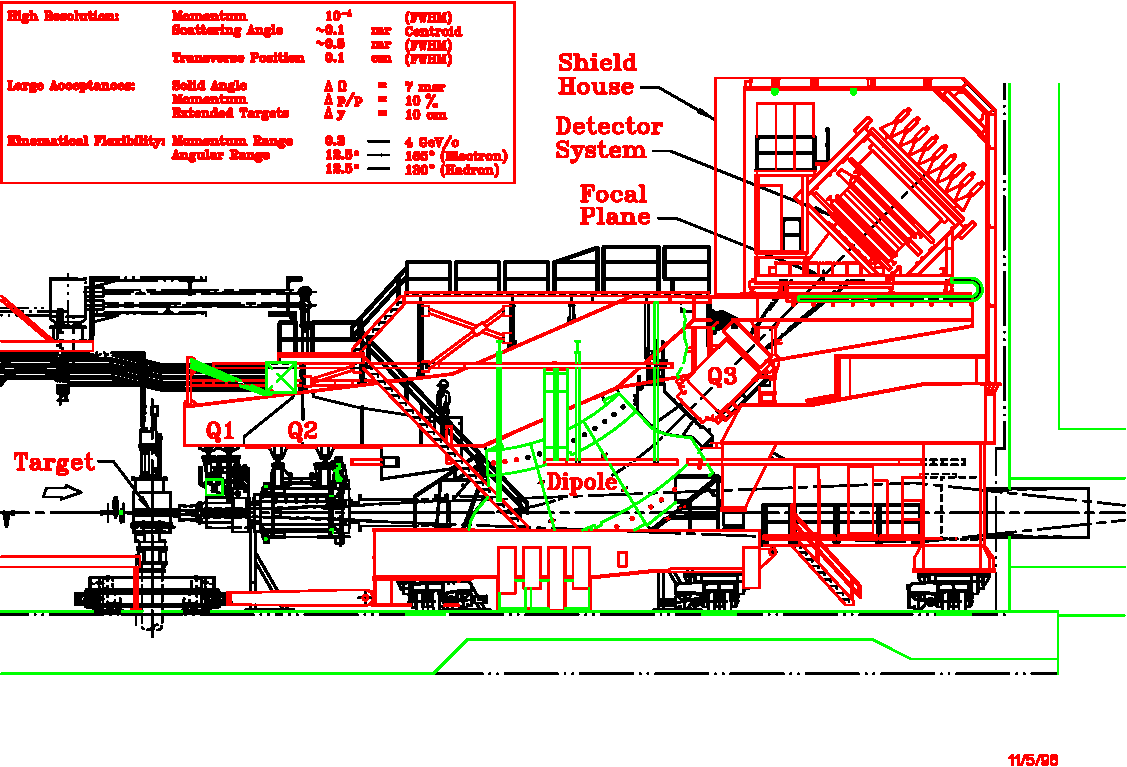
\includegraphics[angle=0,width=0.9\textwidth,clip]{figure0101_r}
\caption[Spectrometers: Elevation View of Hall~A HRS]{A side view of the Hall~A
HRS spectrometer.}  
\label{fig:hrs_ev}
\end{center}
\end{figure}
 
\begin{figure}[tbp]
\begin{center}
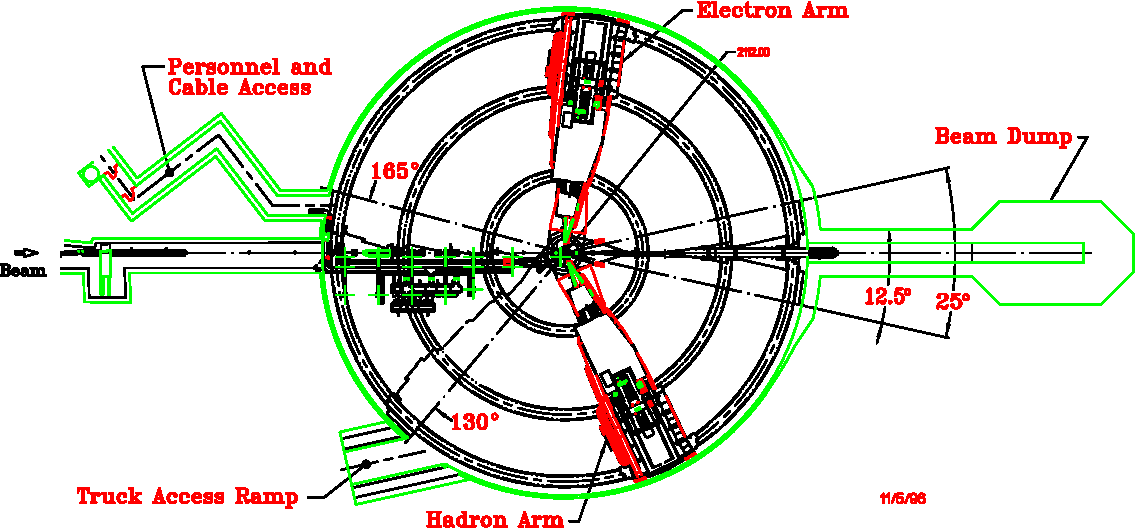
\includegraphics[angle=0,width=0.9\textwidth,clip]{figure0102_r}
\caption[Spectrometers: Plan View of Hall~A]{A bird's eye view of the Hall~A
end-station at TJNAF.}  
\label{fig:hrs_pv}
\end{center}
\end{figure}


A layout of the 4 GeV/c High Resolution Electron Spectrometer is shown 
on Figures~\ref{fig:hrs_pv} and \ref{fig:hrs_ev}.
Its main design characteristics are 
given in the attached table.  The spectrometer has a vertical bending 
plane and 45$^{\circ}$ bending angle.  The QQDQ design includes four 
independent superconducting magnets, three current-dominated 
cos2$\theta $ quadrupoles and one iron-dominated dipole with 
superconducting racetrack coils.  The second and third quadrupoles of 
each spectrometer have sufficiently similar field requirements that they 
are of identical design and construction.  The overall optical length, 
from target to focal plane, is 23.4 m.  Optically, the HRHS 
is essentially identical to HRES. In fact the two spectrometers can be used 
interchangeably to detect either positively or negatively charged particles 
as needed by any particular experiment. They are now commonly refered to 
as ``The Left Arm'' and ``The Right Arms'' rather than ``Hadron'' and ``Electron'' 

The support structure includes all system elements which bear the weight 
of the various spectrometer components and preserve their spatial 
relationship as required for 45$^{\circ}$ vertical bending optics.

The alignment and positioning system includes all the elements which 
measure and adjust the spatial relationship.  The support structure 
consists of the fabricated steel components which support the magnets, 
detector, shield house and associated equipment.  It is composed of the 
box beam, which supports the outer elements in fixed relative position 
atop the dipole; the dipole support bracket, upon which the dipole rests on 
the jacks; the cradle, upon which the dipole rests through the vertical 
positioning system, VPS; and a portion of the shield house load through 
the inboard legs of the gantry; the gantry, which supports the shield 
house and the magnet power supplies; and the bogies, which support the 
cradle-gantry assembly and roll on the floor plates and provide the 
driving power to move the two spectrometer arms.

The detector package (described in detail in Chapter \ref{chap:hrs-det})
is supported on the box beam and is surrounded by 
the shield house.  It must perform two functions, tracking and particle 
identification, PID.  The most important capability of focusing 
spectrometers is measuring precisely the momenta and entrance 
orientations of the tracks.  Momentum resolution of 10$^{-4}$ is 
obtainable, consistent with the resolution of the incident beam.

The actual configuration of the detector package varies from experiment to
experiment. The description given here is only an example of what is possible.
}

\infolevone{
A particle traversing the detector stack 
(Figure~\ref{fig:hrs_electron_det}) encounters two sets of horizontally
mounted, vertical drift wire chambers (x,y) with two planes of 368
wires in each chamber. The track resolution is $\sim$ 100 $\mu$m.  
From the chamber information both 
positions and angles in the dispersive and transverse directions can be 
determined.  The information from these chambers is the principal input 
of the tracking algorithms.

The chambers are followed by a scintillator hodoscope plane designated S1. 
This plastic scintillator array provides the timing reference for 
the drift chambers, and is also used in trigger formation and in combination 
with a second hodoscope pair it can provide time of flight particle 
identification.  These scintillators can also be used to perform crude 
tracking.

The next element encountered by a particle is a gas threshold \Cherenkov{} 
detector.  This is used for particle identification.  This gas threshold \Cherenkov{} detector can be swapped 
against an Aerogel detector, with a similar function.

The second hodoscope plane, S2, is located directly behind the 
gas \Cherenkov{}.  Its function is essentially the same as that of S1.  
In the hadron spectrometer an option exists to have this hodoscope 
pair be preceded by a third chamber, to improve tracking.
 Each of the two spectrometers 
have gas and Aerogel \Cherenkov{} detectors which can be used
 when they are in electron detection mode.

The final elements in the detector stack on HRSE are 
the pre-shower and the total-absorber lead glass shower 
calorimeter.  This is used for energy determination and PID.

\begin{figure}[tbp]
\begin{center}
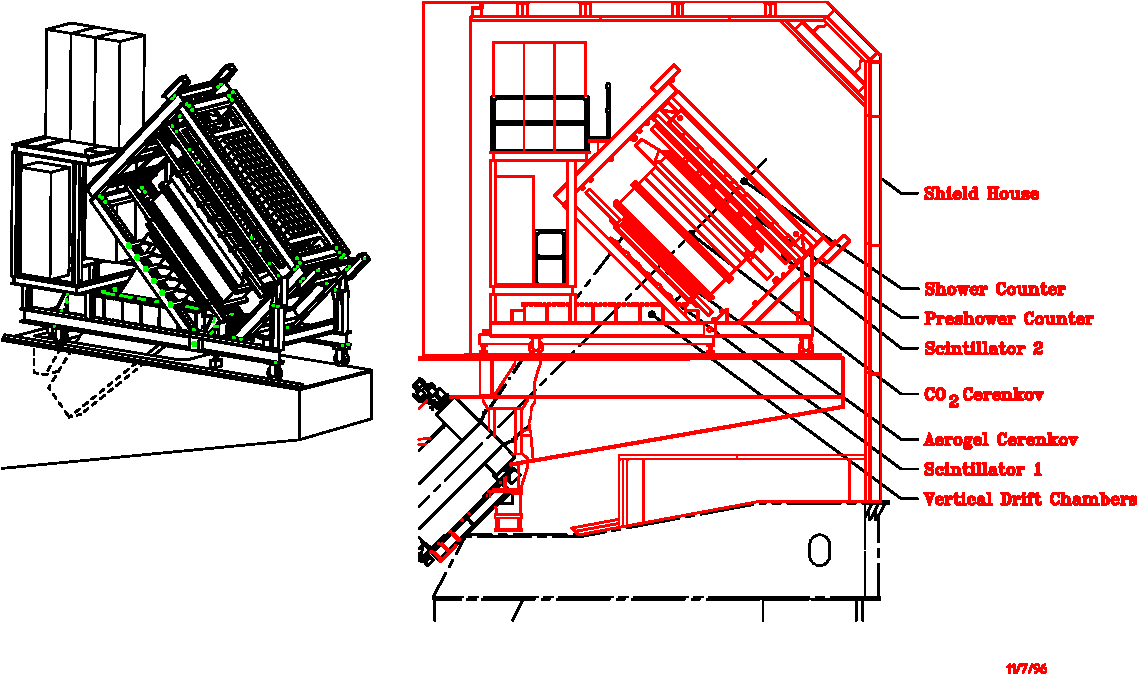
\includegraphics[angle=0,width=\textwidth,clip]{figure0103_r}
{\linespread{1.}
\caption[Spectrometers: Electron Arm Detectors]{The electron spectrometer detector stack.}
\label{fig:hrs_electron_det}}
\end{center}
\end{figure}

\begin{figure}[tbp]
\begin{center}
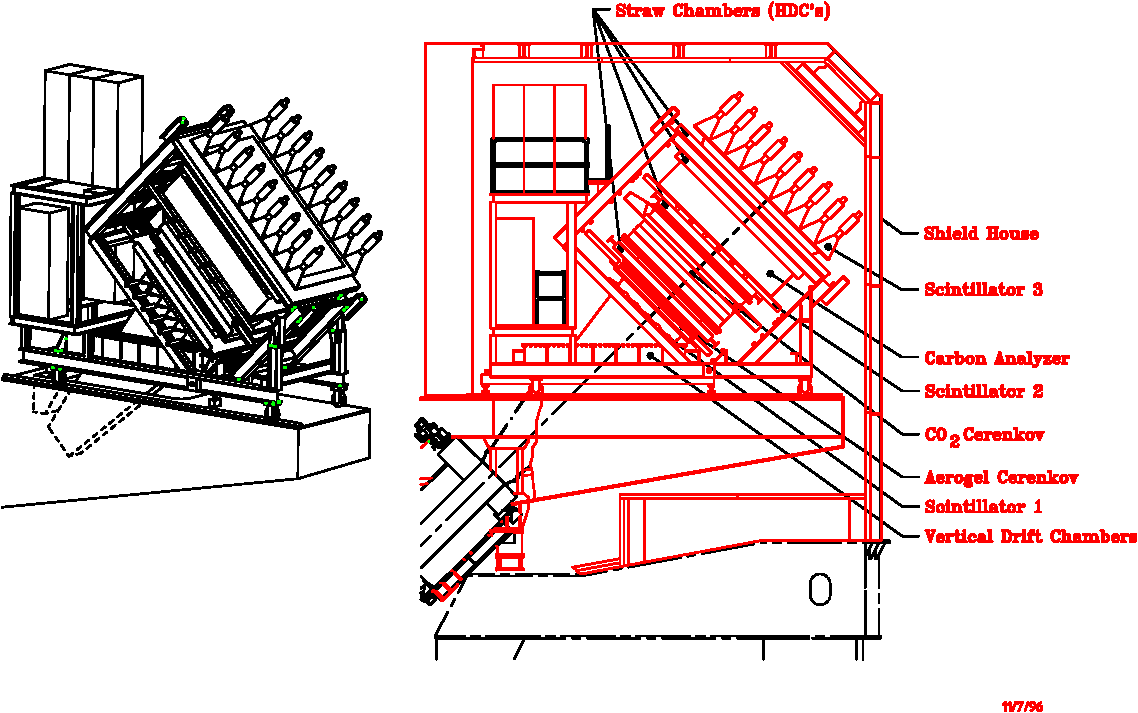
\includegraphics[angle=0,width=\textwidth,clip]{figure0104_r}
{\linespread{1.}
\caption[Spectrometers: Hadron Arm Detectors]{The hadron spectrometer detector stack.}
\label{fig:hrs_hadron_det}}
\end{center}
\end{figure}


The hadron detector is shown schematically in 
Figure~\ref{fig:hrs_hadron_det}.  It consists 
of two sets of (x,y) vertical drift wire chambers identical to those of the 
electron arm.  The remaining part of the detection system is used to 
define the level 1 trigger, as well as for particle identification and 
timing.  It consists of two minimally segmented planes of 
scintillation counters equipped with photomultipliers at both ends, and 
it includes \Cherenkov{} counters (gas CO$_2$ and Aerogel).

In addition, a proton polarimeter is installed in the back of the 
detector package to measure the polarization of the proton using a 
segmented carbon analyzer up to 60 cm in thickness to allow measurements 
over a wide range of proton energies.  A pair of front and a pair of 
rear straw tube wire chambers determine the incident and 
scattered angles, respectively.  The 
polarimeter detectors are dimensioned to accept a 20$^{\circ}$ cone of 
scattered protons.

Several support systems are necessary in addition to the basic 
components mentioned above.  They include gas supply systems for the 
wire chambers, high voltage supplies, readout electronics, a second 
level trigger, software for data analysis and testing, and a remotely 
controllable mechanical system.

For each spectrometer, all detectors are mounted on a 
single rigid support frame along with their associated electronics.  The trigger electronics are located on the support frame, next to the detectors.

To reduce the resolution degrading effects of multiple scattering, the 
entire interior of the spectrometer from the collimator box to the detector hut 
is a vacuum vessel.  The ends of this evacuated volume are capped by 
relatively thin vacuum windows.
}

\begin{safetyen}{0}{0}
\section{High Resolution Spectrometers}
\label{sec:hrs-safety}
\end{safetyen}

The principle concern with the spectrometers is that they are large, 
and have associated vacuum, hydraulic, cryogenic and magnet systems all of 
which can be potentially dangerous.

The bogies which move the massive 1200 ton spectrometers must be 
carefully operated.  Inspection of the floor and wheels to ensure there is no 
debris which the wheels could ride over is mandatory.  Similarly 
personnel need to be aware that the spectrometers are moving so that no one 
inadvertently gets trapped.

The vacuum systems associated with the spectrometers are essentially 
pressure vessels (see Chapter \ref{chap:vacuum} for more details).
Care should be exercised so as not to puncture the 
windows.

The magnets themselves are installed inside cryostats.  These vessels 
are exposed to high pressures and are therefore equipped with safety 
relief valves and burst discs.

The hydraulic system originally intended to operate the vertical positioning system (VPS) 
and the horizontal positioning system (HPS) has effectively been dismantled, after problems were encountered during the initial attempted operation of the system.

The cryogenic system operates at elevated pressure at 4K.  One must 
guard against cold burns and take the normal precautions with pressure 
vessels when operating this system.  Only authorized personnel are permitted to install 
and take out U tubes.

The magnets have a great deal of stored energy as they are large 
inductors. Always make sure people are clear of them and that
the dump resistor is attached to the magnet.

There are several major safety concerns with regards to the detectors, 
namely 1) flammable gas located in the VDC, 2) ODH hazard due to 
CO$_2$ in the \Cherenkov{} counter, 3) high voltage due to the photo 
multipliers on the various detectors and 4) a thin vacuum window 
separating the detector array from the vacuum system in the 
spectrometers.

\infolevltone{
\begin{safetyen}{5}{10}
For more information consult the full OSP manual~\cite{HallAosp}.
\end{safetyen}
} %infolev

\begin{safetyen}{10}{15}
\subsection{Authorized Personnel}
\end{safetyen}

In the event that problems arise during 
operation of the magnets, qualified personnel should be notified
(see Table \ref{tab:hrs:personnel}).  
This includes any prolonged or serious problem with the source of magnet 
cryogens (the ESR).  On weekends and after hours there will be a 
designated individual on call for magnet services.  Any member of the 
Hall A technical staff is qualified to deal with unusual magnet 
situations but in the event of serious problems the technician on
call should be contacted.

\begin{namestab}{tab:hrs:personnel}{HRS: authorized personnel}{%
      HRS: authorized personnel. ''W.B'' stands for the white board 
      in the counting house.}
   \TechonCall{\em Contact}
   \EdFolts{}
   \JackSegal{}
   \HeidiFansler{}
   \JessieButler{}
   \AndrewLumanog{}
   \JasonGlorioso{}
   \MahlonLong{}
\end{namestab}

\infolevone{
\section{The Magnets of HRS}

Each HRS is composed of three superconducting quadrupole magnets, Q1, Q2, 
and Q3, and one superconducting dipole magnet.  The large quadrupoles were 
manufactured for JLab by SIEMENS, the small quadrupole by SACLAY, while 
the dipole was built for JLab by WANG NMR.  The quadrupole magnets are 
referred to as Q1, Q2, and Q3, where a particle first traverses Q1, then 
Q2 and the dipole magnet and finally traverses Q3.

The magnet system is followed by a large steel and concrete detector 
hut, in which all detector elements reside.  Most of the 
detector elements have been built by universities involved in the Hall A 
physics program.

The HRS magnet system is the cornerstone of the Hall A activities.  
Many of the experiments approved in Hall A center on physics at high 
resolution and other short-range phenomena, and rely on a spectrometer 
able to momentum analyze charged particles up to very high momenta.  The 
design value for the maximum momentum accessible to the HRS magnet 
system is 4 GeV/c.
}

\subsection{Magnets and Power Supplies}

\infolevone{
The HRS magnet's are all superconducting and hence their coils must be 
maintained at cryogenic temperatures during operations.  The LHe 
required by the magnets is supplied by the End Station Refrigerator, ESR.

All the HRS magnets cryogenic services are supplied through the overhead 
cryogenic lines.  The distribution network begins at the distribution 
box over the pivot.  This box is connected to the rest of the network 
via the flexible transfer lines over the pivot.  The network is adjacent 
to the upstairs catwalk of the HRS.

Cryogenic information about each magnet is available on the control 
screens in the counting house, one for each magnet.  Normally during run 
periods the control screens are sent upstairs to the Hall A counting 
house and information on all the HRS magnets is available on the HRS 
control screen located in the center of the main console.  The control 
of all magnets is described in a following Section.

The power supplies for the magnets are located on the gantry balcony 
adjacent to the magnets.  The supplies are all cooled with low conductivity water (LCW).
}

\begin{safetyen}{10}{15}

Under no 
circumstances should any panel of any magnet power supply be opened by someone 
other than authorized personnel.  There are also 
signs posted listing the dangers of high magnetic fields.
\end{safetyen}

\infolevone{
A control interface for the power supplies is available through the 
HRS control screen in the Hall A counting house.
}

\infolevone{
\subsection{Quadrupole Magnets}

The quadrupoles provide some of the 
focusing properties of the spectrometer and to a large extent 
its acceptance.  Operating limits imposed on the 
quads are as follows: 1850A for Q2 and Q3 and 3250A 
for Q1.

All three quadrupoles for the HRS spectrometer are warm iron 
superconducting magnets.  The soft iron around the superconducting coil 
enhances the field at the coil center and reduces stray fields.  The 
basic parameters for the first quadrupole, Q1, are an effective length of about 
0.9 $m$, useful aperture of 0.3 $m$ and a field gradient of 9.5 
T/m.  To achieve the lowest possible angle setting of the HRS 
spectrometer (with respect to the beam line) the incident electron beam passes through
a notch in the outer yoke of Q1 when the spectrometer is at
its smallest angle of 12.5$^\circ$ . The 
other two quadrupoles, Q2 and Q3, are essentially identical with an 
effective (magnetic) length of about 1.8 meter, a useful aperture of 
0.6 $m$ and a field gradient of 3.5 T/m.
}

\infolevthree{
The maximum operating currents (assuming a 4 GeV/c momentum particle) 
for the quadrupoles are about 3000 A, 1700 A, and 1600 A, for Q1, Q2, and 
Q3, respectively.  This will render pole field values 
of 1.2, 1.0, and 1.0 T, respectively.  The energy stored in the 
quadrupole fields is sufficient to cause an unrecoverable quench if all 
the energy stored is dumped into the magnets.  Therefore a quench 
protection circuit is incorporated.  However, a quench can only happen 
if the cryomagnets have a helium level below the coil 60\% during operation.

The operating current to the Q1 quadrupole coils is provided by Danfysik 
System 8000 power supplies, which can operate up to 3500 A current and 5 
V.  The power supplies will be cooled with a combined maximum 
water flow of 45 liters per minute.

In addition to the main quadrupole windings, all quadrupoles have 
multipole windings.  To further optimize focusing properties of the HRS 
magnet system, it was intended to operate including some of these multipole 
trim coils in order to reduce higher order aberrations.
The operating current for these multipole corrections would be 
small, only (the multipole corrections are typically less than 2\% of 
the main quadrupole field), of order 50 A. Since the sextupoles were inadvertently 
installed rotated 90 $^\circ$ from their correct
orientation, these trim coils are now considered useless 
and there are at present no plans to use them.

\subsection{Cryogenic Procedures}

The cryogenics control is handled by the JLab Cryogenics Group.  The cryo control coordinator 
can be reached at the CHL (x7405) or by calling the MCC.

\subsection{First Time Startup Check List.}  

See attached check lists for all quadrupole and dipole magnets
 (Tables~\ref{tab:dip_check}, \ref{tab:q1_check}, and \ref{tab:q23_check}).
} %infolev

\infolevone{
\subsection{Dipole Magnet}

The dipole, by virtue of its field index, provides both
dispersion and focusing.  The present operations envelope 
states that the supply for the left HRS dipole may not be
operated at a current above 1800 A (4.4 GeV/c). The supply for the right HRS
dipole may not be operated above 1200 A (3.2 GeV/c), due to complications
caused by an internal short. 

The dipole for the HRS spectrometer is a superconducting, cryostable 
magnet.  Its basic parameters are an effective length of about 6.6 $m$, a 
bend radius of 8.4 $m$, and a gap width of 25 $cm$.  It is configured to 
achieve a 45 degree bending angle for 4 GeV/c momentum particles at a 
central field excitation of 1.6 T.  For the HRS dipole to reach 1.6 T 
an operating current of about 1500 A is required.
} %infolev

\infolevthree{
The dipole has been designed to achieve cryostability up to a field of 2 
T, and this property has been extensively tested up to a field of 1.6 T. 
 The cryostable coils are equipped with an energy removal circuit to 
cover the possibility of an unrecoverable quench.  However, this can 
only happen if the helium level drops below the coil during operation.  
The current to the coils will be provided by a Dynapower Corporation power 
supply, which can operate up to 2000 A and 10 V.  This 
power supply is located on the gantry beside the dipole, and will be 
cooled with a maximum water flow of 35 liters per minute.
The total water flow needed to cool the 4 power 
supplies for the HRS magnet system (dipole and quadrupoles) amounts to 
80 liters per minute, with a supply pressure of cooling water for Hall A 
of 100 psi.
} %infolev

\infolevtwo{
\section{Operation of the HRS Magnets}

\subsection{Introduction}

This is an abbreviated operating manual for 
the HRS superconducting magnets specifically designed for Hall A 
experimenters.  It provides instructions for setting currents, invoking 
NMR field regulation and general system monitoring.  Curious readers are 
directed to the references for more in-depth operating instructions and 
other technical manuals. Copies of the following supporting
documents are available in the Hall A Control Room and through the Hall A webpage
(see Table~\ref{tab:hrs-mag-manuals}).

\begin{table}[htp]
\begin{center}
\begin{tabular}{|l|l|}
\hline
References & \\
\hline 
WANG NMR Dipole & User Manual \\
Dynapower & Instruction Manual \\
Appendix & NMR Tesla meter \\
Appendix & NMR Field Regulation \\
Siemens/Fug & Q2/Q3 Magnet Instrumentation and Power Supplies \\
Saclay/Danfysik & Q1 Power Supply Manual \\
TOSP & HRS Dipole \\
TOSP & HRS Quadrupole Q1 \\
TOSP & HRS Quadrupole Q2, Q3 \\
HRS & SC Dipole Magnet Safety Review Vol. 2 \\
HRS & SC Quad Safety Review Vol. 1 \\ \hline
\end{tabular}
\end{center}
\caption[HRS Magnets: extra manuals]{HRS Magnets: extra manuals available in 
     Hall A Control Room.}
\label{tab:hrs-mag-manuals}
\end{table}

\subsection{Simple HRS Setting (Autopilot Mode)}
\label{sec:hrs-mag-set} 

 The magnets are controlled remotely using EPICS~\cite{EPICSwww} and
 EDM~\cite{EDMwww} GUI, provided that everything is working and power 
 supplies are turned on and ready to go.
 The appropriate interface runs
 on the computer \mycomp{hacsbc2} (see Section \ref{sec:contr-ha-menu}).
 On the ``Hall A General Tools'' control screen, in the upper left, there is 
 a rectangular box for each spectrometer (see Figure~\ref{fig:hrs_mag_cntrl}). 
\begin{figure}
\begin{center}
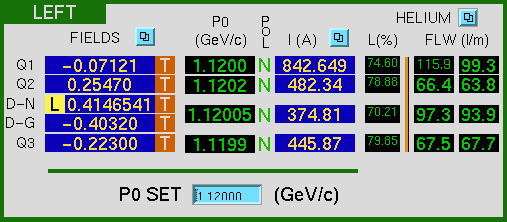
\includegraphics[angle=0,width=0.8\textwidth]{medm_halla_tools_1_cut1}
{\linespread{1.}
\caption[HRS: Magnets control]{A part of ``Hall A General Tools'' screen, 
        used for HRS (left) magnets control.}
\label{fig:hrs_mag_cntrl}}
\end{center}
\end{figure}

This box displays a brief summary of the status of the spectrometer
magnets and their cryogenic systems. The blue fields (with white
numbers) give readbacks of the magnetic fields and currents in each
magnet. The black fields also give readbacks, however in this case if
the text appears green those parameters are OK while if they are red
then that parameter is out of tolerance and may indicate a fault
condition. For example if the helium level goes below a certain point
the magnet will be automatically turned off.  In some cases it may be
desirable to monitor certain critical quantities on a strip chart
(e.g. magnet settings). A strip chart tool is available for this
purpose from the bottom of the ''EOS Menu'' button in the ''MyMenu'' window.

{\bf To set the spectrometers} for a given value of central momentum
(P0) type the desired P0 value into the light blue P0 SET box and hit
return. The magnets will be automatically 
set to the correct
values. All green numbers in the P0 column indicates that the desired
field or current settings have been reached. 

{\bf Caution:} Regarding the
dipoles, in general it's a bad idea to assume that at the first
instant that the P0 display turns green that the desired field has
been reached and you can start taking data. Stable field is in general
not achieved for from 15 to 30 minutes after reaching the nominal
desired field. This settling time depends on the magnet (the right dipole is
slower than the left dipole) and the magnitude of the field change (small
changes settle faster than big changes). Experimenters are advised to
observe both the field reading and current reading on the magnet in
question and verify that things are stable to their satisfaction
before proceeding.
 
\subsection{Powering Up Dipole Magnets:}

Use these instructions to recover from loss of a magnet due to a fault
(e.g. He level or lead flow fault). The order of actions matters. \\
(Contact Tech-On-Call if anything behaves funny or things don't
respond as expected. Sometimes after a trip an access to the Hall is
required to reset things).

\begin{list}{\arabic{enumi}.~}{\usecounter{enumi}\setlength{\itemsep}{-0.15cm}}
   \item Wait for Iout=0 (you can't and don't want to do anything while the magnet is in emergency fast dump mode.)
   \item While waiting, make a log entry re the fault. Give details such as time, coincident activities, and nature of the fault.
   \item Make sure the fault is cleared. (e.g. He level and flow rates returned to normal values and stable)
   \item In the HRS Right (Left) Dipole Systems' control panel:
   \begin{list}{}{\setlength{\itemsep}{-0.15cm}}
      \item[(a)] Press RESET (verify that all faults are cleared in the middle column)
      \item[(b)] Press ON (Display will indicate Power Supply ON and Magnet ENGAGED)
   \end{list}
\end{list}


Power supply and magnet are ready to go. From here you can return 
to "Autopilot Mode" (see Section \ref{sec:hrs-mag-set}).

\subsection{Starting Q1 Power Supply:}

 Do this when a fault causes the power supply to shut off.
 Wait for fault to clear (watch He levels). 
\begin{list}{\arabic{enumi}.~}{\usecounter{enumi}\setlength{\itemsep}{-0.15cm}}
   \item Push POWER OFF/RESET (check all faults cleared)
   \item Select desired polarity
   \item Push POWER ON
   \item Type in Setpoint (Amps) (light blue field) or re-enter P0 in Autopilot Mode.
\end{list}

\subsection{Starting Q2/3 Power Supply:}

 Do this when a fault causes the power supply to shut off.
 Wait for cause of fault to clear (watch He levels). 
 \begin{list}{\arabic{enumi}.~}{\usecounter{enumi}\setlength{\itemsep}{-0.15cm}}
   \item Push RESET 
   \item Select desired polarity
   \item Push ON
   \item Type in Current Set (light blue field) or re-enter P0 in Autopilot Mode.
\end{list}

} %infolev

\subsection{Rotation}
%
% Thanks to John LeRose for Rotation text. 07NOV2013
%
Moving an HRS
Since each HRS weighs in excess of 1,000 tons it is very important that all safety
precautions are carefully adhered to. The good news is they move very slowly (a few degrees/min
maximum), BUT 1,000 tons moving even very slowly is hard to stop. 

Hazards include:
\begin{itemize}
\item{Knocking items over.}
\item{The wheels crushing things (including fingers and toes) on the floor in the path of the 
spectrometer}
\item{Damaging the beamline or other equipment on the floor if one goes to too small 
or too large an angle, or if it just gets pushed around inadvertantly.}
\item{Tearing out of cables etc. physically attached to the superstructure}
\end{itemize}

Hazard mitigations:
\begin{itemize}
\item{Guards on either side of the wheels prevent items from getting under them.}
\item{Large pins in the floor to stop the spectrometer rotated beyond the needed angular range.}
\item{Blinking lights on the spectrometers indicating they are in motion or that motion
is possible (controls engaged etc.)}
\item{During a running experiment the run coordinator and work coordinator should know in advance 
of any moves.  Moves at any other time must be cleared with the Hall work coordinator 
before implementation.}
\item{Careful inspection of the intended path to make sure it is clear. This is part of
the pre-run checklist performed by the technical staff prior to closing the Hall and
a remote camera allows shift worker to inspect the area.}
%
%\item{Any motion that takes a spectrometer inside 14 degrees or outside x degrees
%(x being specified in the pre-run checklist and noted on the whiteboard during a run) 
%must be supervised by a trained Hall A technician.}
\end{itemize}

\infolevone{
Remote Procedure for a shift worker:
\begin{itemize}
\item{Make sure the move is part of the approved runplan (if in doubt, check with the 
run coordinator).}
\item{Check that the pre-run checklist has been completed and note and comply with any 
possible limitations to spectrometer motion (if there is a conflict inform the Run
Coordinator and do not initiate any move until the conflict is cleared).}
\item{Visually inspect the Hall using the closed circuit TV cameras to verify that there
are no obstructions.}
\item{If people are in the Hall wait until they leave (during a Controlled Access MCC keeps
track of people in the Hall). (Maybe we could soften this to "Inform EVERYONE in the Hall of
the move".)}
\item{Activate the spectrometer motion controls (see the Wiki and below) and 
move to the desired angle.}
\item{Deactivate the controls (brakes on, power off, etc.)}
\item{Update the spectrometer position information on the Hall A Controls screen}
\item{Make a halog entry indicating you've moved the spectrometer including from what angle 
to what new angle.}
\end{itemize}

Procedure for a non-run associated move in the Hall:
\begin{itemize}
\item{Inform the work coordinator of the planned move}
\item{Perform a careful visual inspection to verify that the path is clear}
\item{Check to make sure there are no temporary connections to the spectrometer (wires etc.)
that could be damaged during the move.}
\item{Inform everyone in the Hall of the move and check with them re 3.}
\item{Activate the spectrometer motion controls (see the Wiki and below) verify 
that the warning lights are on and move to the desired angle.}
\item{Deactivate the controls (brakes on, power off, etc.).}
\end{itemize}

The full proceedure for moving the spectrometer follows and can also be found on the Hall A wiki.

On hacsbc2, click the red "tool box" icon on the linux taskbar, as above. Choose 
bogies\_SetSpec so that you can determine the angle and vernier setting for the spectrometer.
Enter the spectrometer (L or R), and the angle, and you will get two options for the floor 
mark and the vernier. Generally choose the vernier closer to zero. Center the cameras on the 
desire vernier using the Move+/Move- buttons on the Hall A General Tools screen. The TV monitors 
for these cameras are on the middle shelf, in rack CH01A05.

Choose bogies\_Left (or bogies\_Right) in the tool box to bring up the bogies control screen. 
Click PSM enable and wait a few seconds for PSM OK to read YES. 
Click DM enable and wait a few seconds for DM OK to read YES.
Make sure the velocity is set to 0 and the direction is CW or CCW as desired. Click on Brake Release 
and wait for Brakes OK to read YES.

Click on ClampRelease, set the velocity to 700. Once you see the spectrometer start to move in the 
floor angle camera - you cannot see the spectrometer move in the Hall overview camera, as it only 
moves a few degrees per minute at maximum speed. For the left arm, to move to a larger angle, the 
direction should be CCW, while for the right arm CW moves the spectrometer to larger angle. The 
direction of the spectrometer is reversed by using a negative rpm. Watch the spectrometer motion 
on the cameras. When you are getting close to the desired angle, slow down to about 300 rpm. 
To stop, click on the Clamp Release button and the Brake button. Disable DM and PSM, and disconnect 
to close the GUI. Read off the floor angle mark and vernier, and input the values into the appropriate 
fields in the Alignment section of the Hall A General Tools GUI. 
}









\newpage
\section[Field Monitoring]{Field Monitoring
\footnote{
  $CVS~revision~ $Id: nmr-1999.tex,v 1.4 2003/12/17 03:59:48 gen Exp $ $ 
}
\footnote{Authors: J.LeRose \email{lerose@jlab.org}}
}

The field-monitoring controls are available using the main 
HRS screen%
\infolevtwo{ (see Figure~\ref{fig:hrs_mag_cntrl})%
}. % infolev
The dipoles' field is measured using NMR Teslameters and
field probes.

\infolevone{ 
 
\subsection{ Dipole Field Monitoring Electron Arm}

\noindent {\bf Basic Setup}

Each spectrometer dipole magnet is equipped with a Metrolab PT 4025 
NMR Teslameter, several field probes, and multiplexers (to allow switching 
between the probes).  Details of the operation and theory of operation 
for the Teslameter can be found in its user manual, 
a copy of which is available in the the counting house.
The basic layout is shown in Figure~\ref{fig:nmrbasic}


\begin{figure}
\begin{center}
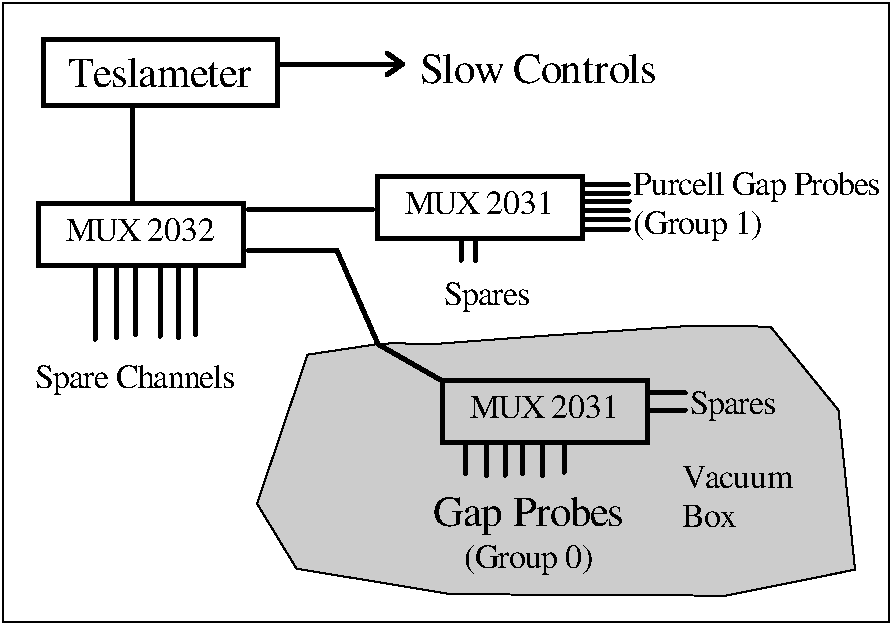
\includegraphics[angle=0,width=15cm,clip]{lerose_fig1}
{\linespread{1.}
\caption[Spectrometers: NMR System Layout]{Basic layout of NMR system}
\label{fig:nmrbasic}}
\end{center}
\end{figure}


 The "Gap Probes" (Group 0 in the controls) are located in two groups 
of three; one group on the low field side of the gap and the other on the high 
field side of the gap.  The groups of three are made up of one each of 
the manufacturer's type 3, 4 \& 5 probes, designed to cover different 
field ranges (see Table \ref{nmr_range}).  The six ``Purcell Gap Probes'' (Group 1 in 
the controls) are located in the Purcell gap of the magnet 
and consists of two each of the above types. {\em Note: Since
the fall of 1998 the multiplexer-multiplexer in both arms,
MUX 2032, has been removed and hence the ``Purcell Gap Probes'' are currently
unavailable. There are no plans to re-install this multiplexer.}

 The "Gap Probes" are equipped with coils which provide a field 
gradient that cancels out the field gradient of the magnet in the vicinity of 
the probe.  These gradient compensating coils are part of a simple circuit 
that is completely independent of the Teslameter.  The basic circuit for 
the compensating coils is shown in Figure~\ref{fig:nmrcir}


\begin{figure}
\begin{center}
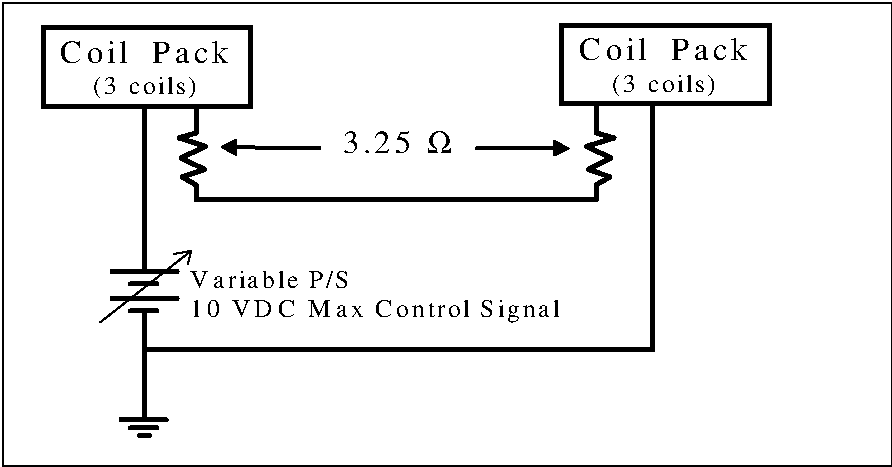
\includegraphics[angle=0,width=10cm,clip]{lerose_fig2}
{\linespread{1.}
\caption[Spectrometers: NMR Gradient Compensation]{Gradient Compensating Circuit.}
\label{fig:nmrcir}}
\end{center}
\end{figure}


%\snfig{figs/lerose_figcce.eps}{Control Voltage calibration for
%Electron Dipole }{nmrcomp4}{5in}

\begin{figure}
\begin{center}
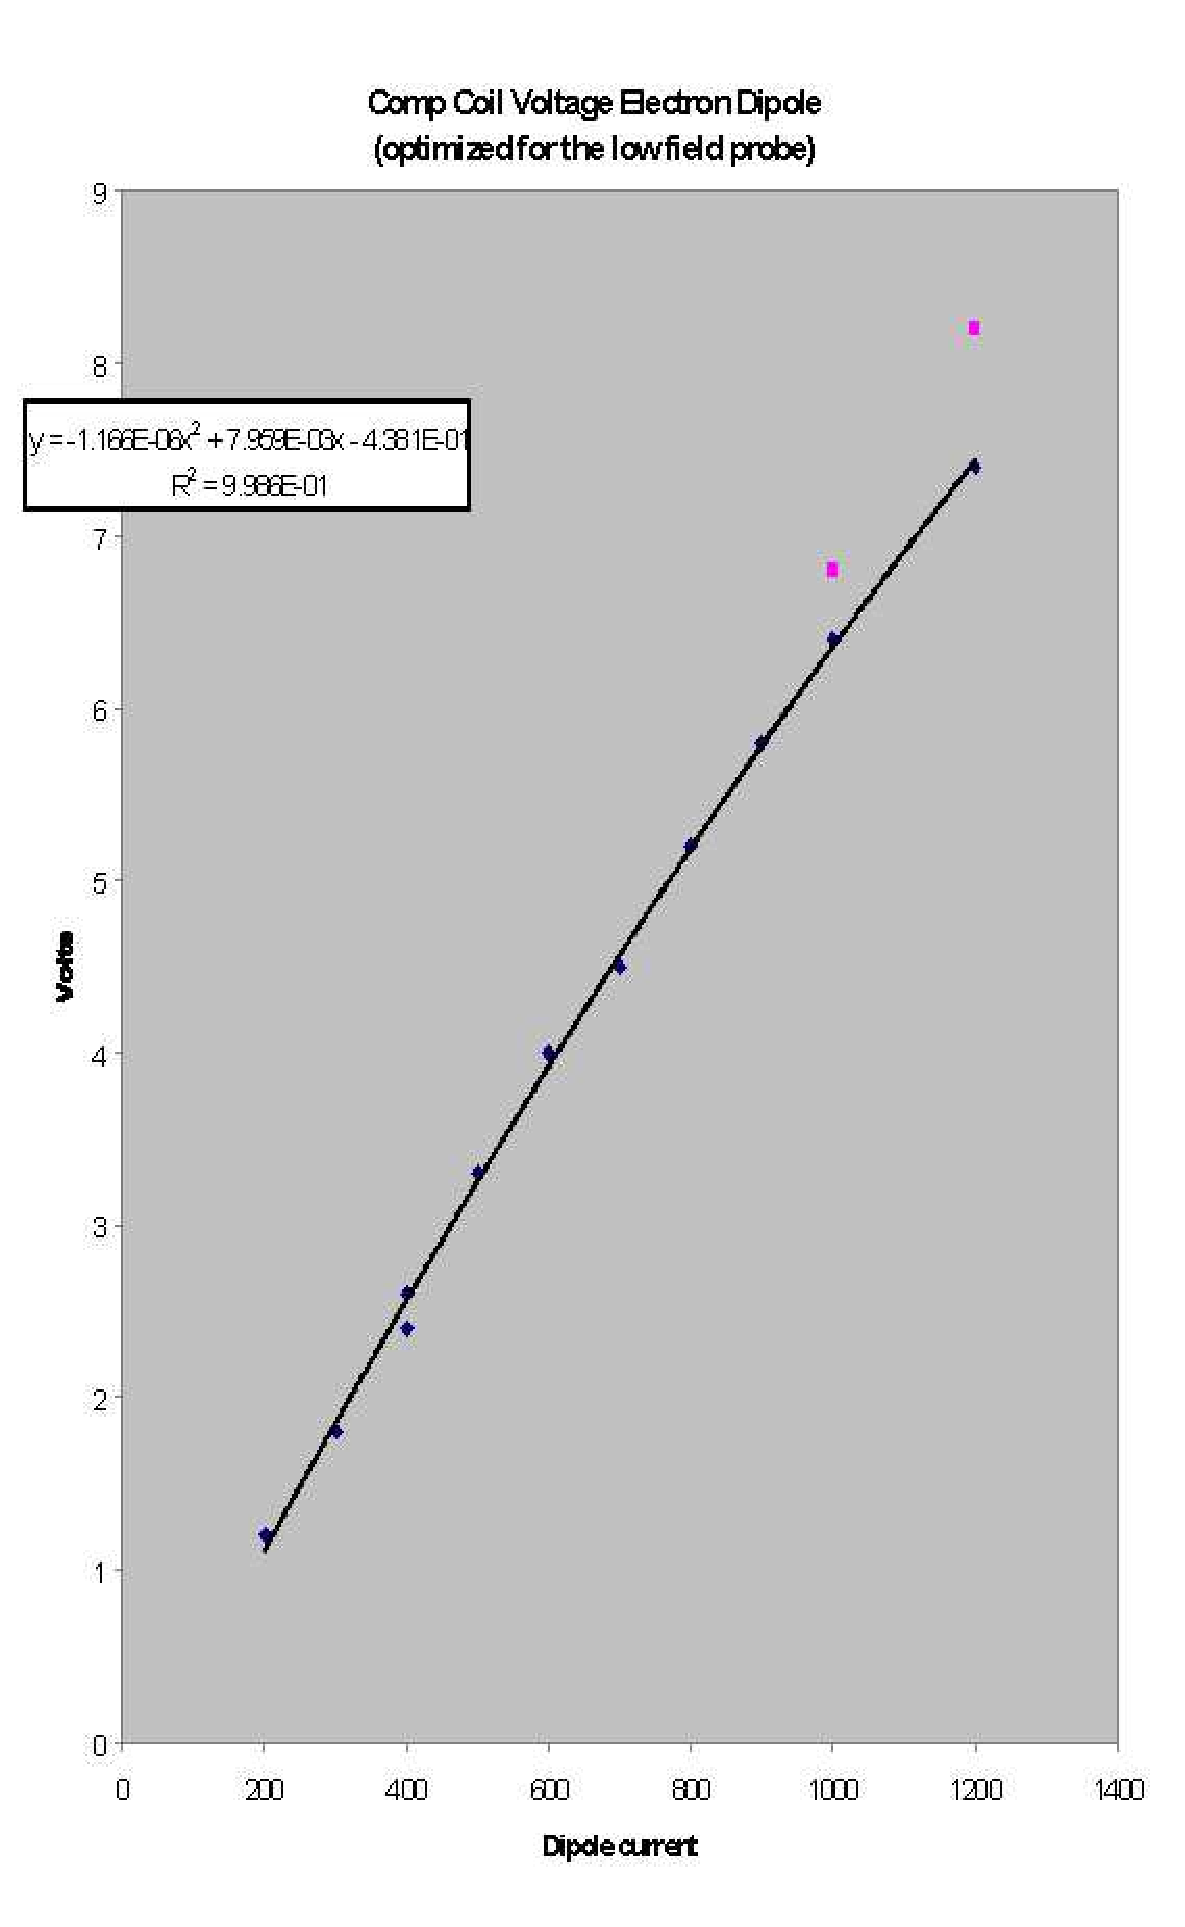
\includegraphics[angle=0,height=20cm,clip]{lerose_figcce}
{\linespread{1.}
\caption[Spectrometers: Control Voltage Calibration for Left Dipole]{Control Voltage calibration for the Left Dipole.}
\label{fig:nmrcomp4}}
\end{center}
\end{figure}

%\snfig{figs/lerose_figcch.eps}{Control Voltage calibration for
%Hadron Dipole }{nmrcomp5}{5in}
\begin{figure}
\begin{center}
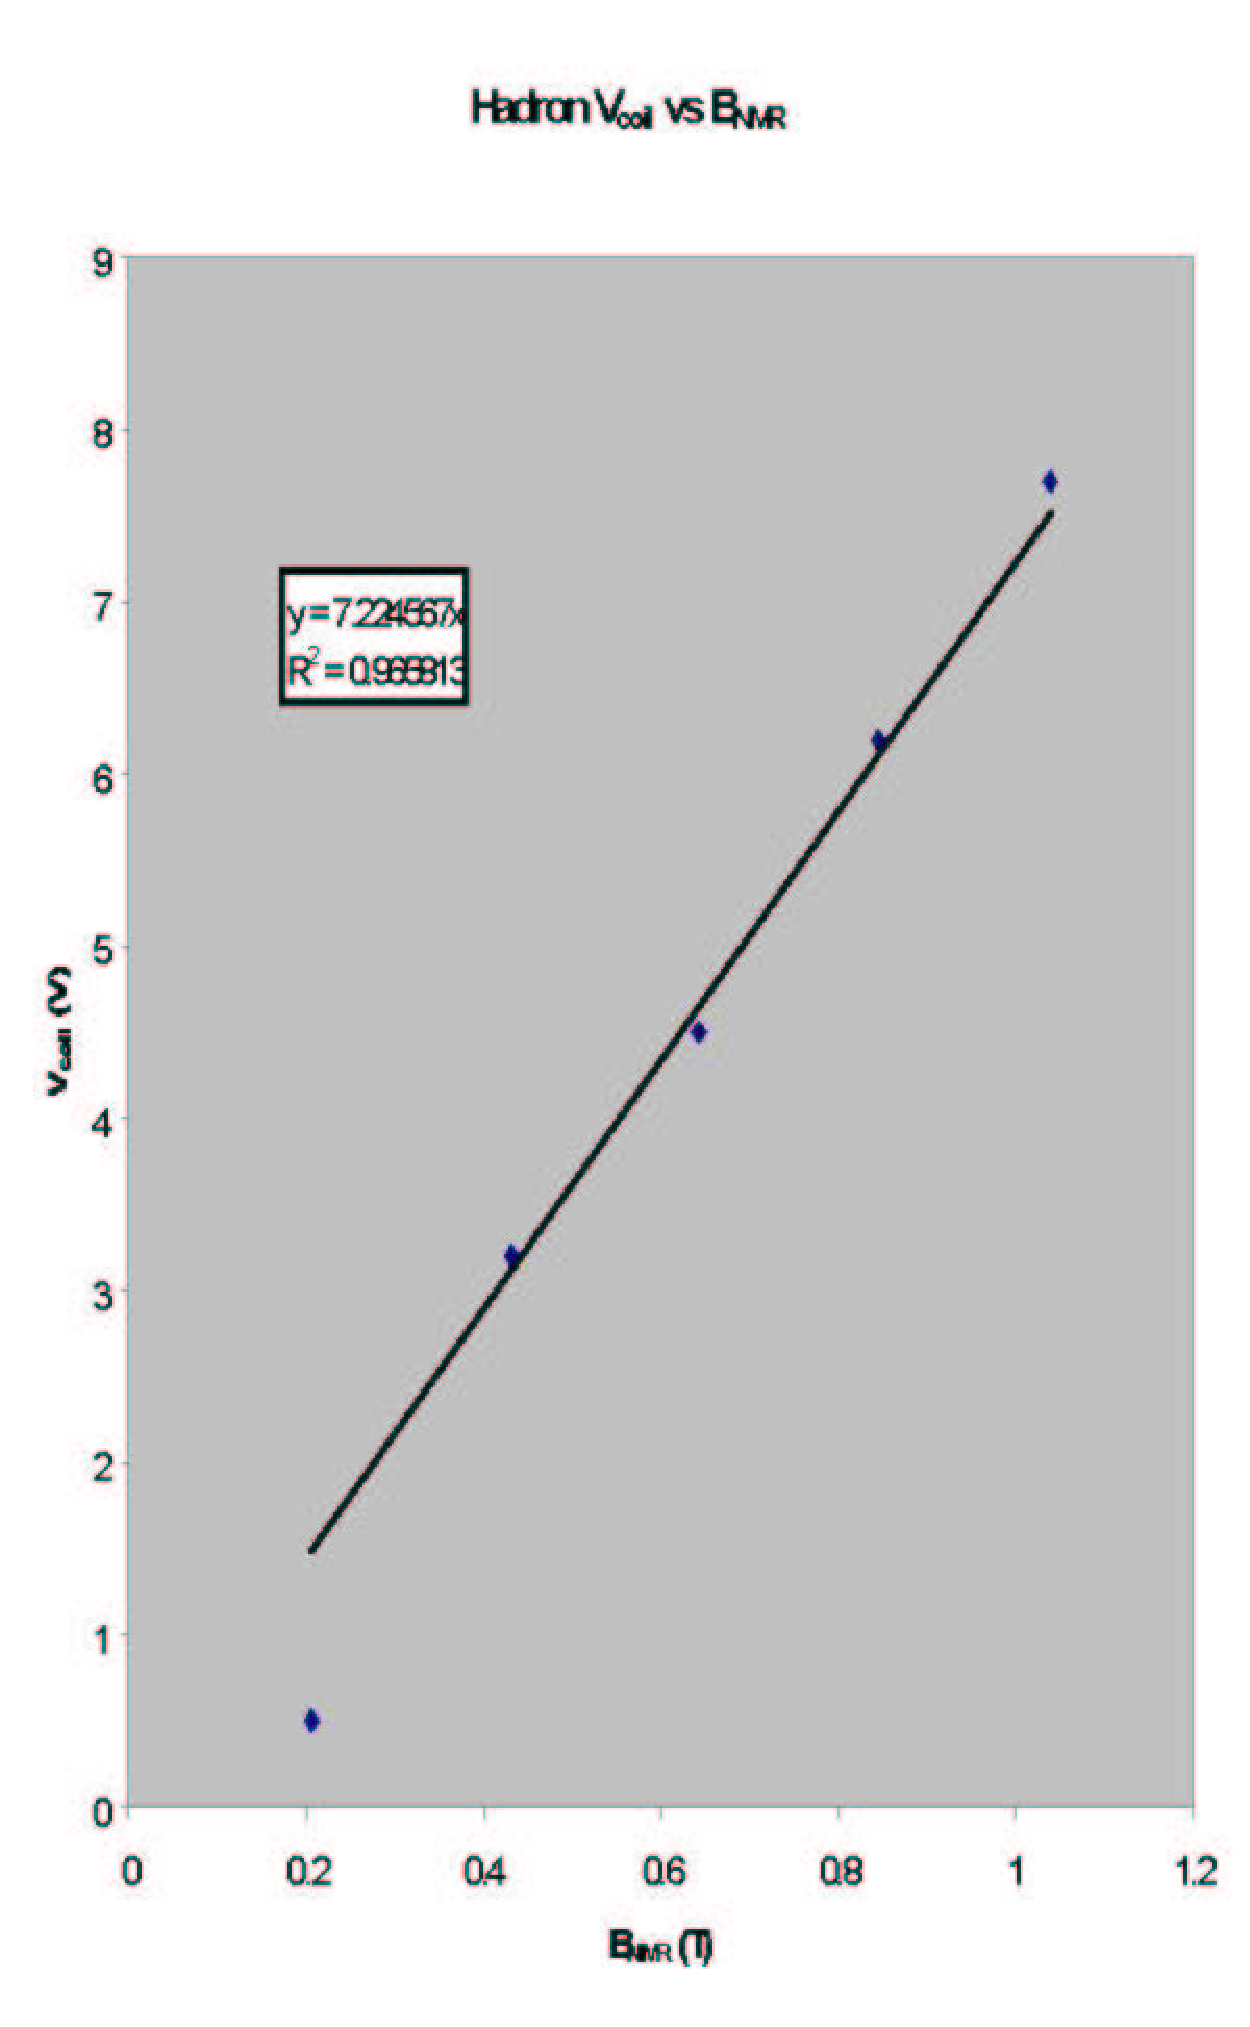
\includegraphics[angle=0,height=20cm,clip]{lerose_figcch}
{\linespread{1.}
\caption[Spectrometers: Control Voltage Calibration for Right Dipole] {Control Voltage calibration for the Right Dipole.}
\label{fig:nmrcomp5}}
\end{center}
\end{figure}

%\snfig{./figs/lerose_fig7.eps}{DAC Calibration for manual operation of NMR probes}{nmr_dac}{9in}
\begin{figure}
\begin{center}
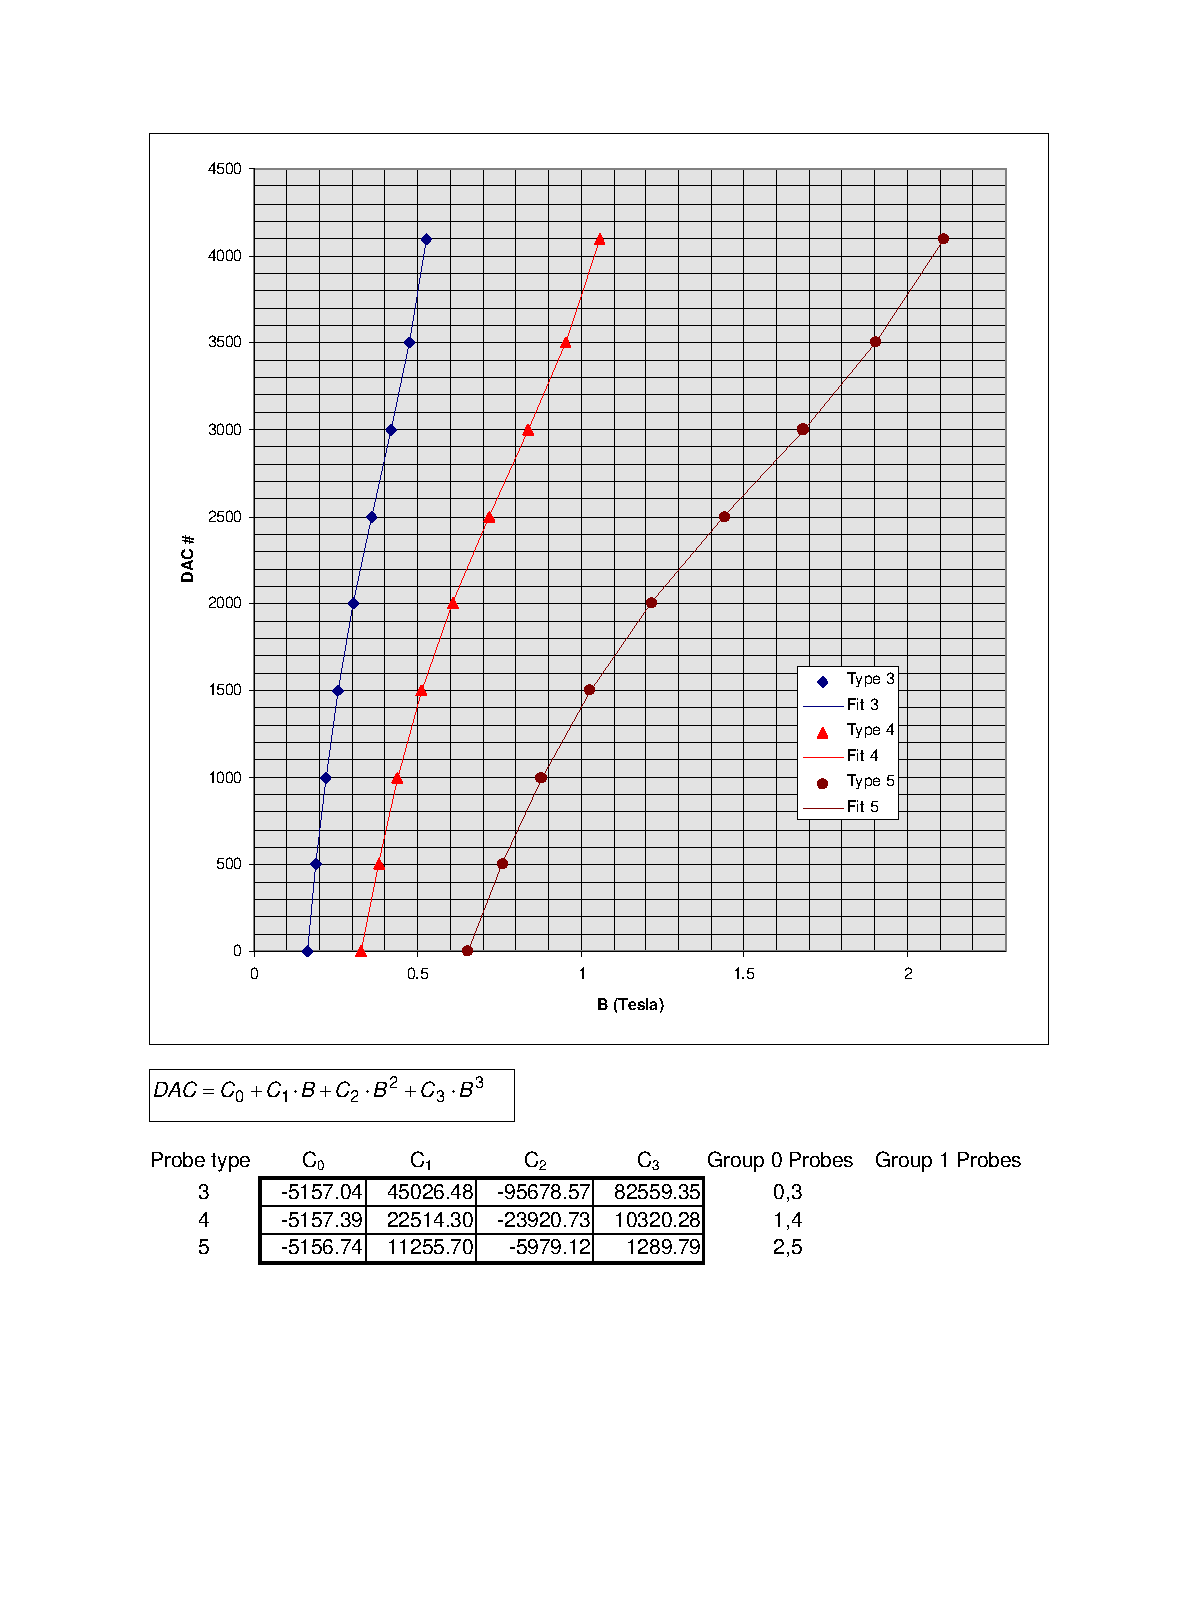
\includegraphics[angle=0,height=20cm,clip]{lerose_fig7}
{\linespread{1.}
\caption[Spectrometers: NMR Probe DAC Calibration]{DAC Calibration for manual operation of NMR probes.}
\label{fig:nmr_dac}}
\end{center}
\end{figure}

The following graphs (see Figures~\ref{fig:nmrcomp4} 
and ~\ref{fig:nmrcomp5}),can be used to determine optimum values for the 
compensating coil control voltage.  It should be noted that the setting 
of the compensating coil current is not very critical in most cases.  In 
general if you're within 10\% of the correct value everything should 
work fine.



\begin{table}
\begin{center}
\begin{tabular}{|cc|} \hline
Probe Type & Field Range (T) \\ \hline 
3 & 0.17 - 0.52 \\
4 & 0.35 - 1.05 \\
5 & 0.70 - 2.10 \\ \hline
\end{tabular}
\caption[Spectrometers: Dipole NMR Probe Field Ranges]{Dipole NMR probe field ranges}
\label{nmr_range}
\end{center}
\end{table}

} %infolev

\infolevtwo{
\subsection{NMR Operating Procedure}

When running in Autopilot mode (see: Simple Spectrometer Field Setting) the 
compensating coil voltage is set automatically and the probe appropriate for 
the field desired is selected. The gaussmeter is placed in SEARCH Mode and the 
dipole power supply software regulator is turned on. In this case the dipole current is 
adjusted to achieve the desired field. The user should just stand 
back and let it work. What follows are instructions for using
the NMR gaussmeter in situations where Autopilot doesn't work or
some special supplemental measurements are required. 

 In principle it is possible to make the field measurements using the 
SEARCH mode in the Teslameter.  In this mode you select a probe and the 
meter explores the whole field range of the probe until it finds and 
"locks" on the resonant signal indicating that it has a field 
measurement.  A ``lock" is indicated on the controls display by an ``L'' to 
the left of the field values.  This has the advantage of simplicity but in practice can 
be time consuming and doesn't always work.  The problem being, in 
situations where there is a lot of noise mixed in with the signal, the 
circuitry has problems distinguishing the signal from the noise and gets 
lost before it ever finds a lock.  The problem is exacerbated when the 
field being measured is at the high end of the probe's range.  In this 
case the search starts at the low end and keeps getting hung up on the 
noise and never gets to the field range of interest.  The solution to 
this problem is to tell the device approximately what field it's looking 
for and use the AUTO mode to find the lock.  In the procedure below that 
is what we will be doing.

In any case, for ``gap probes" (group 0) you must energize and adjust 
the gradient compensating coils for the field ranges to be measured before 
trying to make a measurement.

For studies involving 
10\% changes in the field settings the compensating coil current can be 
set once and left alone.


\noindent\underline{\bf Recommended Procedure:}(turn the {\bf SOFTWARE REGULATOR OFF} for all 
non-autopilot field measurements)\\
For group 0 probes set compensating coils appropriately (see figures).\\
Put the meter in MANUAL mode with SEARCH OFF \\
Select a probe \underline{\bf and} polarity (\underline{\bf Group 0:  
Probes 0, 1, 2 negative; Probes 3, 4, 5 positive}) \\
Type in the appropriate DAC number for the field range being measured (see below) \\
Select AUTO and wait for a lock (indicating a valid field reading) \\
Verify that you have a good lock by checking the oscilloscope for a 
clear resonant signal. \\
If you have problems see the table listing problems and possible 
solutions.

\noindent\underline{\bf Selecting DAC Number}

In selecting the DAC number to use for the field of interest use 
either the graph in Figure~\ref{fig:nmr_dac} or the polynomial at the bottom of the same figure.

\pagebreak
\noindent{\bf Problems and Solutions}\\
\begin{table}[htb]
\begin{tabular}{|p{0.4\textwidth}|p{0.55\textwidth}|}\hline
Symptom & Diagnosis and Cure \\ \hline\hline
Weird numbers on displays, controls for all magnets fouled up 
& Need to reboot.  See instructions below. \\ \hline
NMR Teslameter does not respond to commands and display shows all zeros. 
& Meter's communications are somehow hung up. Push {\bf RESET}. \\ \hline
%Will not lock & Very high noise level makes resonance hard to find. \\
%Still 
Will not lock 
& Very high noise level makes resonance hard to find. Search for the resonance manually by 
  adjusting the DAC in manual mode until you see the resonant signal.  (It helps if you know 
  what field you expect so you'll know where to look). \\ \hline
You find resonance manually but still can't get a lock 
& Check probe polarity. Try decreasing and increasing DAC number by 1. Optimize signal 
  by adjusting compensating coils. \\ \hline
Can't find resonance manually 
& Try a different probe.  Use readings from other probes to tell you where to look for 
 the resonance with the probe that's giving you trouble.  Make sure
 compensating coils are energized properly.  Make sure magnet is on. \\ \hline\hline
\end{tabular}
\caption[NMR: Problems and solutions]{NMR: Problems and solutions}
\label{tab:nmr-problems-solutions}
\end{table}

\begin{table}[ht]
\begin{center}
\begin{tabular}{|p{0.3\textwidth}|p{0.3\textwidth}|p{0.3\textwidth}|}\hline
Problems & Explanation & Action \\ \hline
NMR not locked but current is changing in the right direction 
& Normal operation for large field changes  
& Wait. (see above) \\ \hline
NMR locked but current going in the wrong direction.
& Normal operation. 
& Wait. \\ \hline
NMR locked but field not correct and current not changing 
& Field regulation is disabled or software is confused.
& Check that field regulation is enabled. Enter desired field value or one
  very near the desired value again. \\ \hline
NMR field display freezes. (Usually but not always shows  -\#.0000000)
& NMR Gaussmeter is not communicating with software.
& Push {\bf RESET}. \\ \hline
\end{tabular}
\end{center}
\caption[NMR troubleshhoting]{NMR troubleshooting
}
\label{tab:hrs_nmr_2}
\end{table}

} %infolev

\begin{safetyen}{10}{15}
\subsection{Authorized Personnel}
\end{safetyen}

The individuals shown in Table \ref{tab:nmr:personnel} are responsible for NMR operation problems.

\begin{namestab}{tab:nmr:personnel}{NMR: authorized personnel}{%
      NMR: authorized personnel.}
  \JavierGomez{\em Contact}
  \JohnLeRose{}
\end{namestab}



\newpage
\section[Collimators and Sieve Slits]{Collimators and Sieve Slits
\footnote{
  $CVS~revision~ $Id: slit.tex,v 1.5 2003/12/13 06:23:38 gen Exp $ $ 
}
\footnote{Authors: J.LeRose \email{lerose@jlab.org}}
}

Both spectrometers have front-end devices for calibrating the optical
properties of the spectrometers. These are known as the collimator boxes.
These boxes are positioned between the scattering chamber and the 
first quadrupoles (Q1). Each box is carefully aligned and rigidly attached
to the  entrance flange of the Q1 of the respective spectrometer.  The boxes are
part of the vacuum system of the spectrometer.
In the septum configuration sieve slits and collimators are installed and removed manually.

Inside each box a ladder is mounted which is guided by a linear bearing
and moved up and down by a ball screw. On this ladder 3 positions are 
available to insert collimators. Below this ladder
a special valve is mounted that can isolate the vacuum in the spectrometer
from the target system. This valve should be activated when it is moved
in front of the holes connecting the box with spectrometer and target chamber.
\infolevone{
A schematic view of the collimator box is shown in Fig.~\ref{fig:coll}.

\begin{figure}
\begin{center}
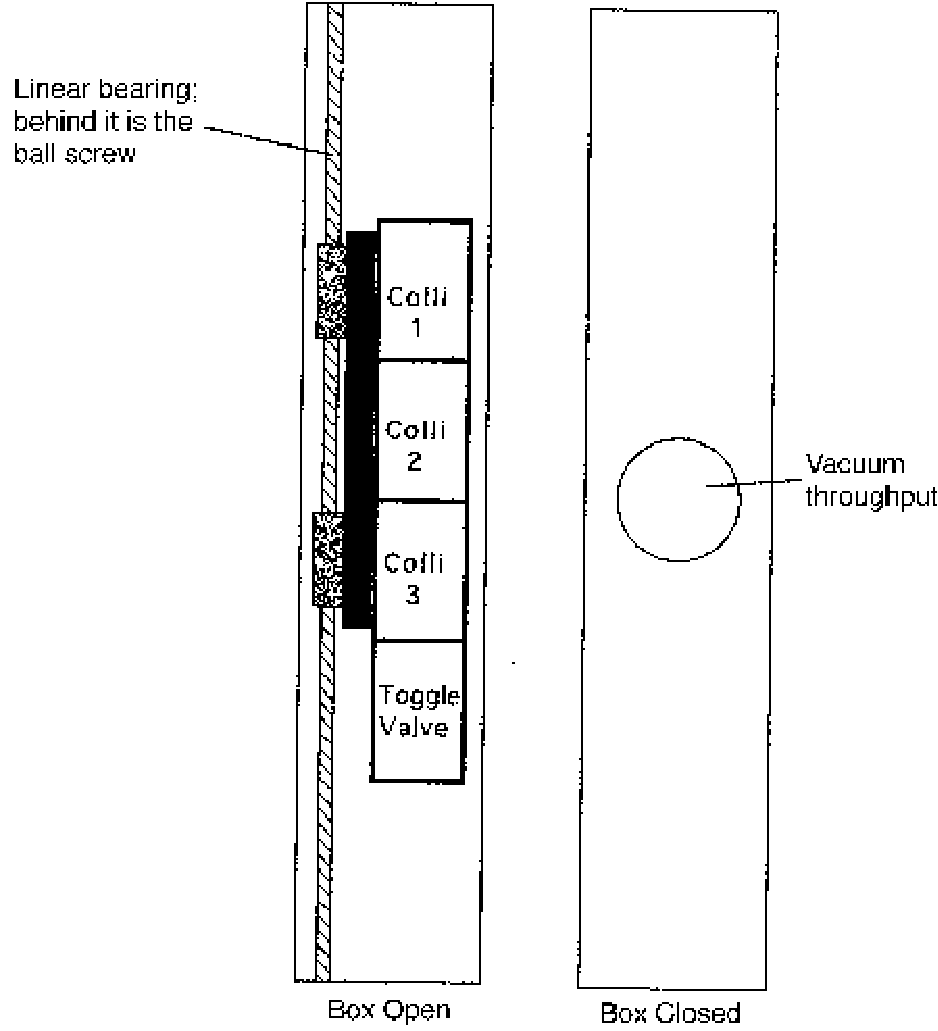
\includegraphics[angle=0,width=13cm,clip]{collimator_clip}
{\linespread{1.}
\caption[Spectrometers: Collimator Box Schematic]{Schematic layout of the collimator box.}
\label{fig:coll}}
\end{center}
\end{figure}
} %infolev

Vacuum requirement is $10^{-6}$ Torr. The material for the box is 
aluminum. It is possible to open one side of the box so that
collimators can be exchanged. The
reproducibility of collimator positions after moving
the ladder and/or after replacing a collimator is
better than 0.1 mm in horizontal and vertical direction.
The dimensions of the box are
roughly height=175 cm , width=35 cm and depth=15 cm.
The tolerance in the dimension
of the 7 msr collimator hole is $\pm0.5$ mm in each direction. 
The tolerance in the position
of each of the sieve-slit holes is $\pm0.1$ mm in each direction.

\infolevone{
\begin{figure}
\begin{center}
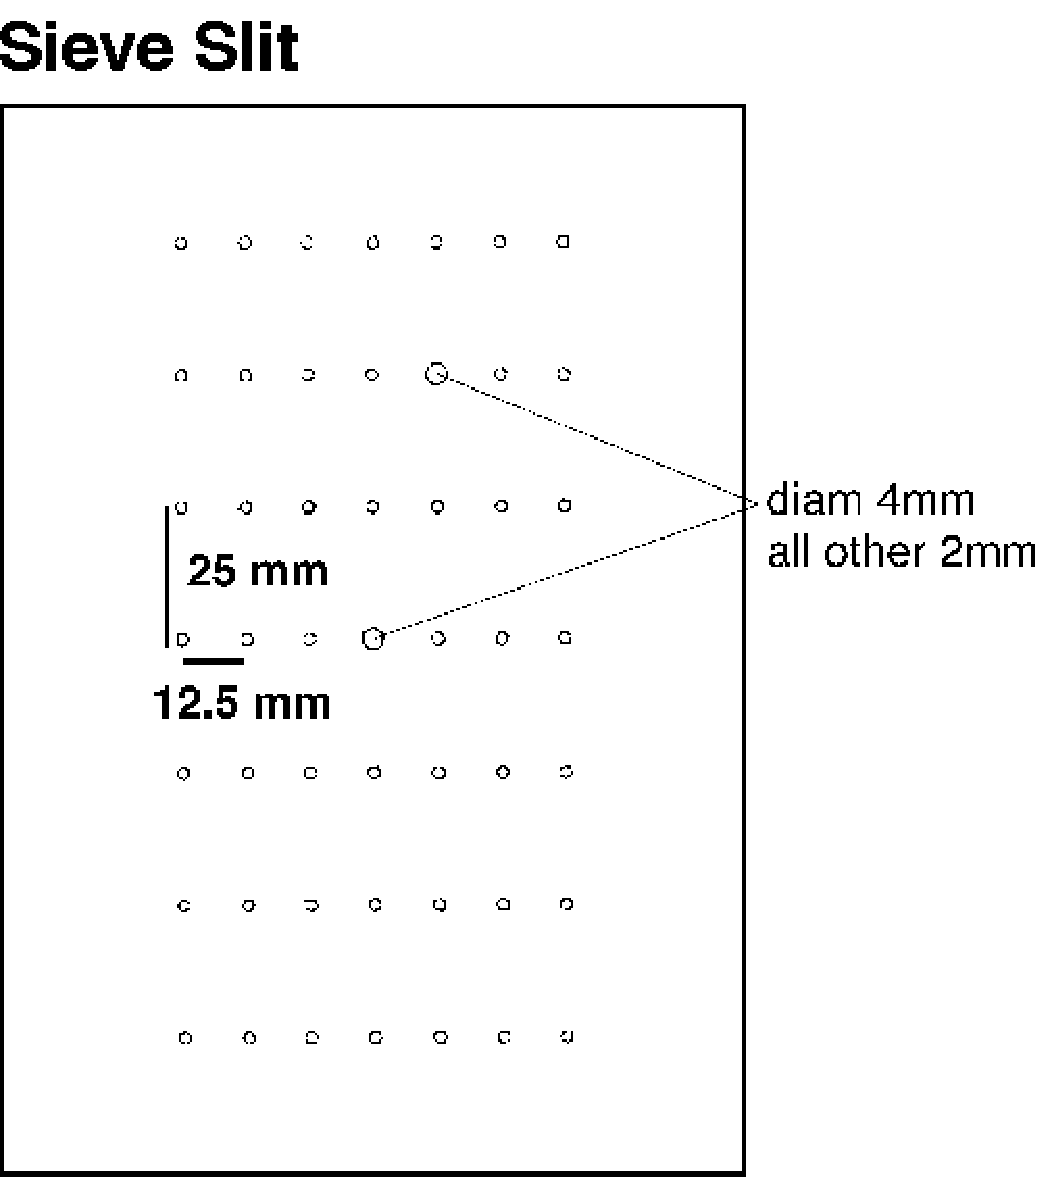
\includegraphics[angle=0,width=13cm,clip]{sieveslit}
{\linespread{1.}
\caption[Spectrometers: Sieve Slit]{Sieve slit collimator for optics calibration.}
\label{fig:sieve}}
\end{center}
\end{figure}
} %infolev
A typical sieve slit collimator 
\infolevone{(shown in Fig.~\ref{fig:sieve})
} %infolev 
consists of a plate of roughly 14 cm x 20 cm containing 49 holes
positioned in a regular 7x7 pattern. This slit is made out of 5
mm thick tungsten.
The holes have a diameter of 2 mm except for the central one and one positioned
off-diagonal which have a diameter of 4 mm. The horizontal distance between the
holes is 12.5 mm while the vertical distance is 25.0 mm.
%
%To get the latest information on the dimensions and locations of the collimators see 
%the Hall A homepage on the web%
%\htmladdnormallinkfoot{}{\url{
%http://hallaweb.jlab.org/
%}}.

To get the latest information on the dimensions and locations of the collimators see 
the Hall A homepage on the web%
\htmladdnormallinkfoot{}{\url{
http://hallaweb.jlab.org/
}}.

\begin{safetyen}{10}{15}
\subsection{Safety Assessment}

The collimator boxes form part of the vacuum system for each spectrometer. All hazards
identified in section spectrometer vacuum section applies to the collimator box as well.

In addition, safe access to the top of
the collimator boxes is needed  during manual operation of the box as outlined below.
Due to the proximity of the collimator boxes to the scattering chamber, and Q1 quadrupoles,
all necessary safety precautions with regards to vacuum windows, electrical power cables, 
cryogenic transfer lines, and high magnetic field should be taken. The same precautions also apply 
to the collimators and sieves in the septum configuration. In that case the sieve and collomators
can be considered part of the beamline. A survey and
appropriate RADCON designated proceedures must be followed when dealing with septum sieves 
and collimators.
\end{safetyen}

\infolevtwo{
\subsection{Operating Procedure}
Slit position is changed remotely from the standard Hall A control screen.
In the case of a spectrometer configuration involving the septum magnets collimators and sieves are
changed manually in the Hall.
} %infolev

\subsection{Authorized  Personnel} 

\begin{itemize} 
\item[~]E. Folts - x7857 (mechanical and vacuum systems).
\item[~]J. Gomez - x7498 (computer controls and electrical systems).
\end{itemize} 

% ===========  CVS info
% $Header: /group/halla/analysis/cvs/tex/osp/src/hrs/slit.tex,v 1.5 2003/12/13 06:23:38 gen Exp $
% $Id: slit.tex,v 1.5 2003/12/13 06:23:38 gen Exp $
% $Author: gen $
% $Date: 2003/12/13 06:23:38 $
% $Name:  $
% $Locker:  $
% $Log: slit.tex,v $
% Revision 1.5  2003/12/13 06:23:38  gen
% Septum added. Name tables. Polishing
%
% Revision 1.4  2003/12/05 06:49:07  gen
% infolevels added, polishing
%
% Revision 1.3  2003/06/06 16:13:37  gen
% Revision printout changed
%
% Revision 1.2  2003/06/05 23:30:00  gen
% Revision ID is printed in TeX
%
% Revision 1.1.1.1  2003/06/05 17:28:31  gen
% Imported from /home/gen/tex/OSP
%
%  Revision parameters to appear on the output

\newpage
\infolevtwo{
\section[Spectrometer Alignment]{Spectrometer Alignment
\footnote{
  $CVS~revision~ $Id: AlignmentOps.tex,v 1.8 2003/12/17 03:59:48 gen Exp $ $ 
}
\footnote{Authors: J.Gomez \email{gomez@jlab.org}}
}

At present, the systems implemented to determine the alignment of each spectrometer
(roll, vertical angle/pointing and horizontal angle/pointing) without the help of the
Accelerator Division Survey group are limited to roll, vertical angle and horizontal angle.
All alignment information is displayed in the ``ALIGNMENT'' mosaic of the ``Hall A
General Tools'' EDM screen%
\infolevtwo{ (see Fig.~\ref{fig:medm-hlamain-tools})}
(``EOS Menu'' $-->$ ``EDM (HLA Main)'' $-->$ ``Hall A Main Menu'' $-->$ ``Tools'').

A bi-axial inclinometer is used to determine the roll and vertical angle (also known as pitch)
of each spectrometer. These inclinometers are attached to the back of the dipoles at the power
supply platform level. The raw inclinometer measurements, in Volts,
are displayed as ``Tilt X'' and ``Tilt Y''. The inclinometer temperature is also given
(`` Tilt T''), in degree Celsius. From these values, the ``ROLL'' and ``PITCH'' values are
calculated.
Agreement between the inclinometer readings and survey measurements
are better than $\pm$ 0.1 mrad over all presently available history.

The horizontal spectrometer angle is determined from floor marks set in
place by the survey group. Floor marks have been placed every 0.5 $^\circ$ covering the useful range of
both spectrometers.
There are two concentric rings of floor marks in the hall. We will concentrate in the
inner ring which covers the angular range of both spectrometers. The outer ring is
similar.
The inner-ring floor marks are located at a distance of $\sim$10 $m$ from the target center.
A ruler attached to each spectrometer dipole runs over the floor marks and it acts as a vernier to interpolate
between marks. The location of a given floor mark on the ruler can be viewed from the Hall A Counting
House through a TV camera (labeled ``Front Camera'') .
The camera is able to move along the length of the ruler so that any
parallax effect can be eliminated. The camera motion is controlled from the ``Tools'' screen
through two push buttons (``FRONT CAMERA'' - ``MOVE +'' and ``MOVE --'').
Two fields in the ``ALIGNMENT'' mosaic
(``Flr Mrk'' and ``Vernier'') allow to input
the values read from the TV monitor. The effective spectrometer angle is then calculated and displayed
as ``Angle''. The application ``HRS Floor Marks'' calculates the floor mark and vernier value
to which the spectrometer should be set
to obtain a given angle. Spectrometer horizontal angle surveys and floor mark determinations
agree to $\pm$ 0.2 mrad.

\newpage
\begin{safetyen}{10}{15}
\subsection{Authorized  Personnel} 
\end{safetyen}
The authorized personnel is shown in table \ref{tab:align:personnel}.
\begin{namestab}{tab:align:personnel}{HRS alignment: authorized personnel}{%
      HRS alignment: authorized personnel.}
  \JessieButler{\em Contact}
\end{namestab}

} %infolev


% ===========  CVS info
% $Header: /group/halla/analysis/cvs/tex/osp/src/hrs/all.tex,v 1.3 2003/06/06 15:44:08 gen Exp $
% $Id: all.tex,v 1.3 2003/06/06 15:44:08 gen Exp $
% $Author: gen $
% $Date: 2003/06/06 15:44:08 $
% $Name:  $
% $Locker:  $
% $Log: all.tex,v $
% Revision 1.3  2003/06/06 15:44:08  gen
% Revision printout changed
%
% Revision 1.2  2003/06/05 23:30:00  gen
% Revision ID is printed in TeX
%
% Revision 1.1.1.1  2003/06/05 17:28:31  gen
% Imported from /home/gen/tex/OSP
%
%  Revision parameters to appear on the output

%\chapter{High Resolution Spectrometers (HRS)}
\graphicspath{{hrs/figs/}}
\renewcommand{\dirfig}[0]{hrs/figs}
\renewcommand{\dircur}[0]{hrs}

\infolevone{
\chapter[High Resolution Spectrometers (HRS)]{High Resolution Spectrometers (HRS)
}
\footnote{Authors: J.LeRose \email{lerose@jlab.org}}
}
\label{chap:hrs}

\infolevone{
\section{Overview}
   
The Hall A spectrometers and associated instrumentation are designed to 
perform high resolution and high accuracy experiments.  The goal is to 
achieve a missing mass resolution of $\sim$ 200-500 keV to clearly 
identify the nuclear final state.  An absolute accuracy of $\sim$ 1\% is 
also required by the physics program planned in the Hall, which implies 
$\sim$ 10$^{-4}$ accuracy in the determination of particle momenta and 
$\sim$ 0.1 mr in the knowledge of the scattering angle.

The instruments needed are a high resolution electron spectrometer 
(HRES) and a high resolution hadron spectrometer (HRHS), both with a 
large angular and momentum acceptance.

\begin{figure}[tbp]
\begin{center}
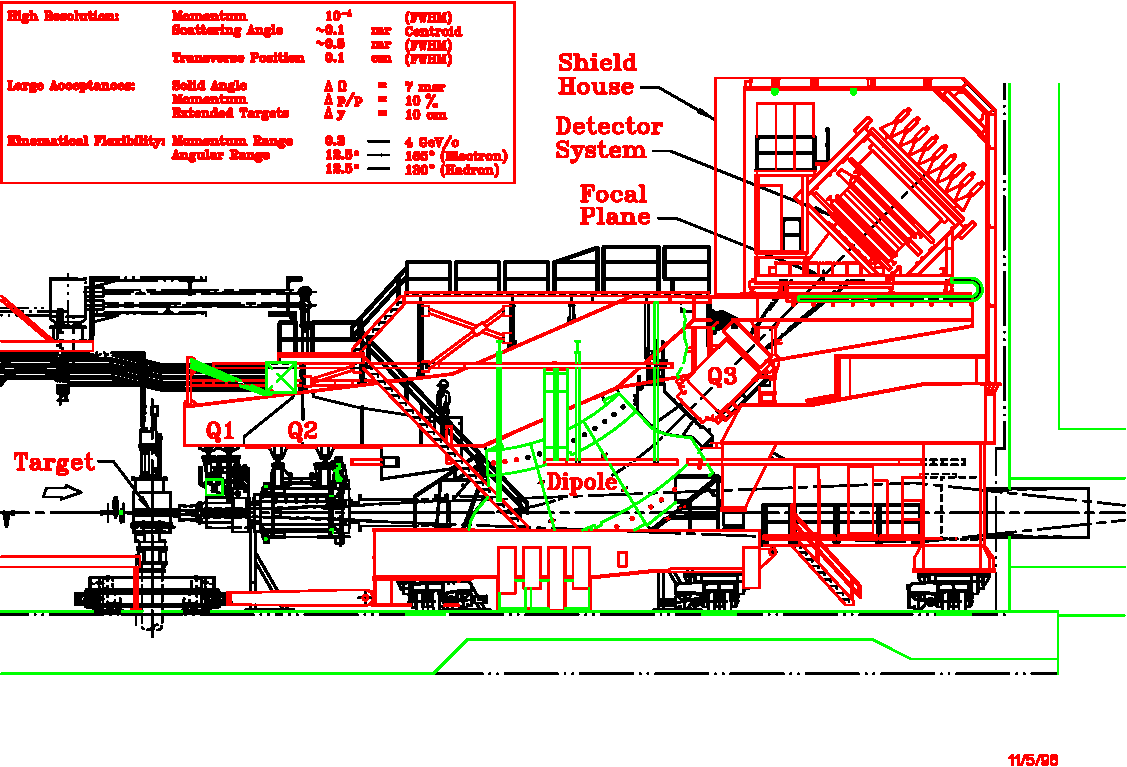
\includegraphics[angle=0,width=0.9\textwidth,clip]{figure0101_r}
\caption[Spectrometers: Elevation View of Hall~A HRS]{A side view of the Hall~A
HRS spectrometer.}  
\label{fig:hrs_ev}
\end{center}
\end{figure}
 
\begin{figure}[tbp]
\begin{center}
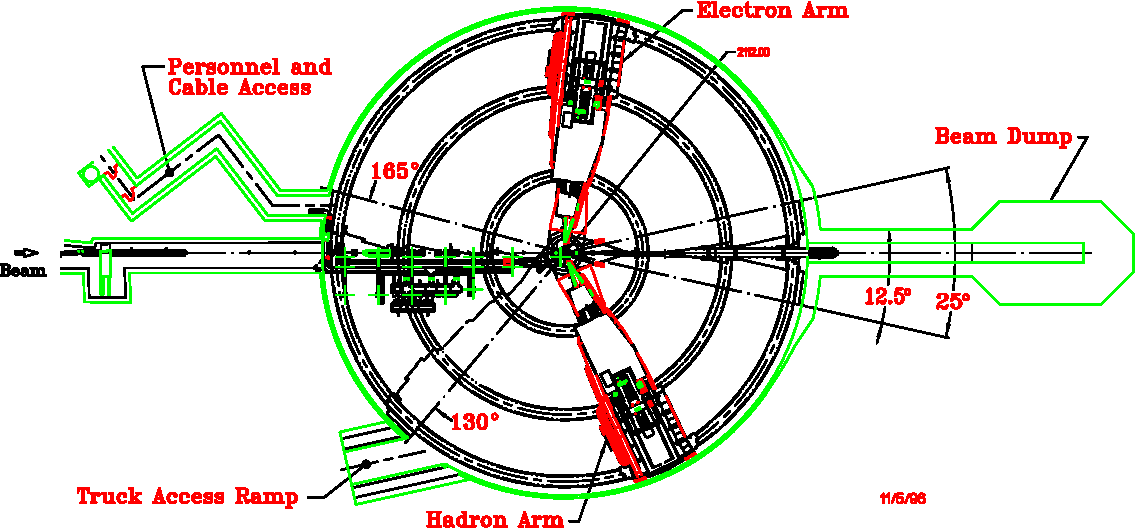
\includegraphics[angle=0,width=0.9\textwidth,clip]{figure0102_r}
\caption[Spectrometers: Plan View of Hall~A]{A bird's eye view of the Hall~A
end-station at TJNAF.}  
\label{fig:hrs_pv}
\end{center}
\end{figure}


A layout of the 4 GeV/c High Resolution Electron Spectrometer is shown 
on Figures~\ref{fig:hrs_pv} and \ref{fig:hrs_ev}.
Its main design characteristics are 
given in the attached table.  The spectrometer has a vertical bending 
plane and 45$^{\circ}$ bending angle.  The QQDQ design includes four 
independent superconducting magnets, three current-dominated 
cos2$\theta $ quadrupoles and one iron-dominated dipole with 
superconducting racetrack coils.  The second and third quadrupoles of 
each spectrometer have sufficiently similar field requirements that they 
are of identical design and construction.  The overall optical length, 
from target to focal plane, is 23.4 m.  Optically, the HRHS 
is essentially identical to HRES. In fact the two spectrometers can be used 
interchangeably to detect either positively or negatively charged particles 
as needed by any particular experiment. They are now commonly refered to 
as ``The Left Arm'' and ``The Right Arms'' rather than ``Hadron'' and ``Electron'' 

The support structure includes all system elements which bear the weight 
of the various spectrometer components and preserve their spatial 
relationship as required for 45$^{\circ}$ vertical bending optics.

The alignment and positioning system includes all the elements which 
measure and adjust the spatial relationship.  The support structure 
consists of the fabricated steel components which support the magnets, 
detector, shield house and associated equipment.  It is composed of the 
box beam, which supports the outer elements in fixed relative position 
atop the dipole; the dipole support bracket, upon which the dipole rests on 
the jacks; the cradle, upon which the dipole rests through the vertical 
positioning system, VPS; and a portion of the shield house load through 
the inboard legs of the gantry; the gantry, which supports the shield 
house and the magnet power supplies; and the bogies, which support the 
cradle-gantry assembly and roll on the floor plates and provide the 
driving power to move the two spectrometer arms.

The detector package (described in detail in Chapter \ref{chap:hrs-det})
is supported on the box beam and is surrounded by 
the shield house.  It must perform two functions, tracking and particle 
identification, PID.  The most important capability of focusing 
spectrometers is measuring precisely the momenta and entrance 
orientations of the tracks.  Momentum resolution of 10$^{-4}$ is 
obtainable, consistent with the resolution of the incident beam.

The actual configuration of the detector package varies from experiment to
experiment. The description given here is only an example of what is possible.
}

\infolevone{
A particle traversing the detector stack 
(Figure~\ref{fig:hrs_electron_det}) encounters two sets of horizontally
mounted, vertical drift wire chambers (x,y) with two planes of 368
wires in each chamber. The track resolution is $\sim$ 100 $\mu$m.  
From the chamber information both 
positions and angles in the dispersive and transverse directions can be 
determined.  The information from these chambers is the principal input 
of the tracking algorithms.

The chambers are followed by a scintillator hodoscope plane designated S1. 
This plastic scintillator array provides the timing reference for 
the drift chambers, and is also used in trigger formation and in combination 
with a second hodoscope pair it can provide time of flight particle 
identification.  These scintillators can also be used to perform crude 
tracking.

The next element encountered by a particle is a gas threshold \Cherenkov{} 
detector.  This is used for particle identification.  This gas threshold \Cherenkov{} detector can be swapped 
against an Aerogel detector, with a similar function.

The second hodoscope plane, S2, is located directly behind the 
gas \Cherenkov{}.  Its function is essentially the same as that of S1.  
In the hadron spectrometer an option exists to have this hodoscope 
pair be preceded by a third chamber, to improve tracking.
 Each of the two spectrometers 
have gas and Aerogel \Cherenkov{} detectors which can be used
 when they are in electron detection mode.

The final elements in the detector stack on HRSE are 
the pre-shower and the total-absorber lead glass shower 
calorimeter.  This is used for energy determination and PID.

\begin{figure}[tbp]
\begin{center}
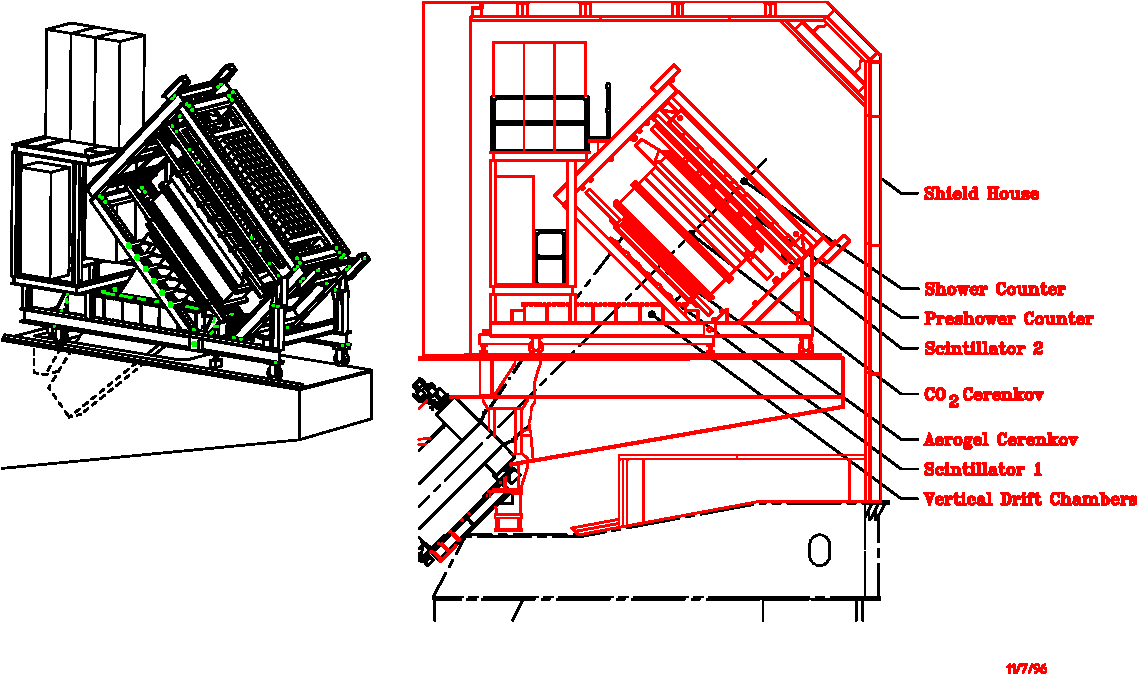
\includegraphics[angle=0,width=\textwidth,clip]{figure0103_r}
{\linespread{1.}
\caption[Spectrometers: Electron Arm Detectors]{The electron spectrometer detector stack.}
\label{fig:hrs_electron_det}}
\end{center}
\end{figure}

\begin{figure}[tbp]
\begin{center}
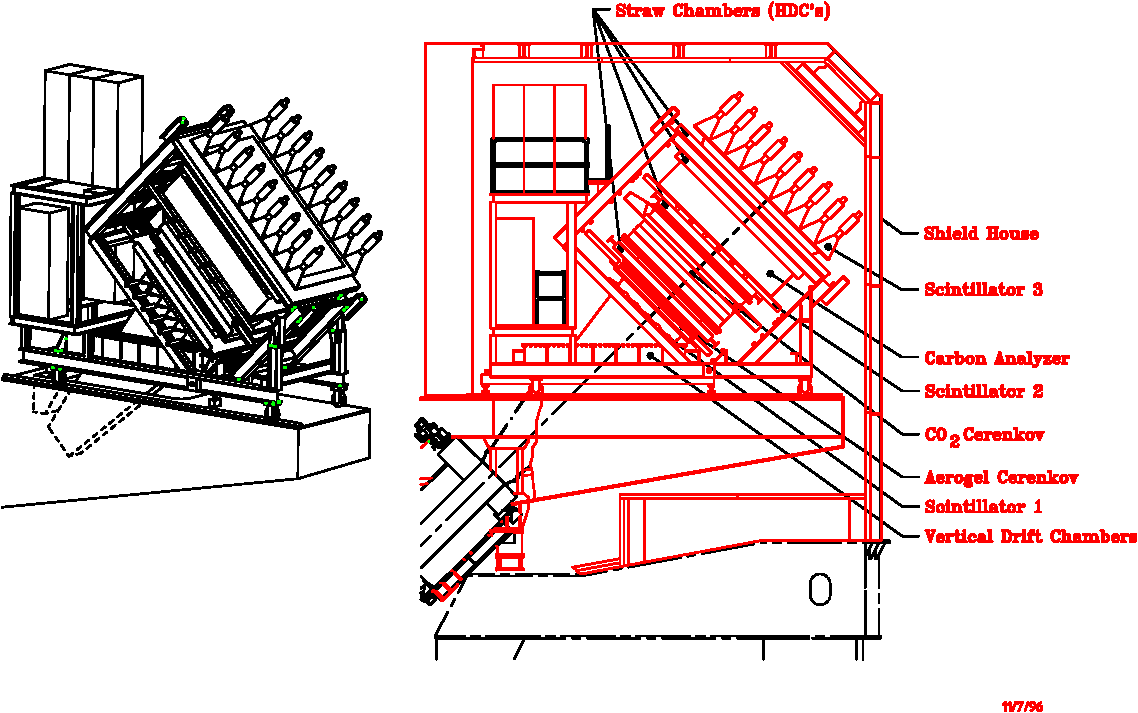
\includegraphics[angle=0,width=\textwidth,clip]{figure0104_r}
{\linespread{1.}
\caption[Spectrometers: Hadron Arm Detectors]{The hadron spectrometer detector stack.}
\label{fig:hrs_hadron_det}}
\end{center}
\end{figure}


The hadron detector is shown schematically in 
Figure~\ref{fig:hrs_hadron_det}.  It consists 
of two sets of (x,y) vertical drift wire chambers identical to those of the 
electron arm.  The remaining part of the detection system is used to 
define the level 1 trigger, as well as for particle identification and 
timing.  It consists of two minimally segmented planes of 
scintillation counters equipped with photomultipliers at both ends, and 
it includes \Cherenkov{} counters (gas CO$_2$ and Aerogel).

In addition, a proton polarimeter is installed in the back of the 
detector package to measure the polarization of the proton using a 
segmented carbon analyzer up to 60 cm in thickness to allow measurements 
over a wide range of proton energies.  A pair of front and a pair of 
rear straw tube wire chambers determine the incident and 
scattered angles, respectively.  The 
polarimeter detectors are dimensioned to accept a 20$^{\circ}$ cone of 
scattered protons.

Several support systems are necessary in addition to the basic 
components mentioned above.  They include gas supply systems for the 
wire chambers, high voltage supplies, readout electronics, a second 
level trigger, software for data analysis and testing, and a remotely 
controllable mechanical system.

For each spectrometer, all detectors are mounted on a 
single rigid support frame along with their associated electronics.  The trigger electronics are located on the support frame, next to the detectors.

To reduce the resolution degrading effects of multiple scattering, the 
entire interior of the spectrometer from the collimator box to the detector hut 
is a vacuum vessel.  The ends of this evacuated volume are capped by 
relatively thin vacuum windows.
}

\begin{safetyen}{0}{0}
\section{High Resolution Spectrometers}
\label{sec:hrs-safety}
\end{safetyen}

The principle concern with the spectrometers is that they are large, 
and have associated vacuum, hydraulic, cryogenic and magnet systems all of 
which can be potentially dangerous.

The bogies which move the massive 1200 ton spectrometers must be 
carefully operated.  Inspection of the floor and wheels to ensure there is no 
debris which the wheels could ride over is mandatory.  Similarly 
personnel need to be aware that the spectrometers are moving so that no one 
inadvertently gets trapped.

The vacuum systems associated with the spectrometers are essentially 
pressure vessels (see Chapter \ref{chap:vacuum} for more details).
Care should be exercised so as not to puncture the 
windows.

The magnets themselves are installed inside cryostats.  These vessels 
are exposed to high pressures and are therefore equipped with safety 
relief valves and burst discs.

The hydraulic system originally intended to operate the vertical positioning system (VPS) 
and the horizontal positioning system (HPS) has effectively been dismantled, after problems were encountered during the initial attempted operation of the system.

The cryogenic system operates at elevated pressure at 4K.  One must 
guard against cold burns and take the normal precautions with pressure 
vessels when operating this system.  Only authorized personnel are permitted to install 
and take out U tubes.

The magnets have a great deal of stored energy as they are large 
inductors. Always make sure people are clear of them and that
the dump resistor is attached to the magnet.

There are several major safety concerns with regards to the detectors, 
namely 1) flammable gas located in the VDC, 2) ODH hazard due to 
CO$_2$ in the \Cherenkov{} counter, 3) high voltage due to the photo 
multipliers on the various detectors and 4) a thin vacuum window 
separating the detector array from the vacuum system in the 
spectrometers.

\infolevltone{
\begin{safetyen}{5}{10}
For more information consult the full OSP manual~\cite{HallAosp}.
\end{safetyen}
} %infolev

\begin{safetyen}{10}{15}
\subsection{Authorized Personnel}
\end{safetyen}

In the event that problems arise during 
operation of the magnets, qualified personnel should be notified
(see Table \ref{tab:hrs:personnel}).  
This includes any prolonged or serious problem with the source of magnet 
cryogens (the ESR).  On weekends and after hours there will be a 
designated individual on call for magnet services.  Any member of the 
Hall A technical staff is qualified to deal with unusual magnet 
situations but in the event of serious problems the technician on
call should be contacted.

\begin{namestab}{tab:hrs:personnel}{HRS: authorized personnel}{%
      HRS: authorized personnel. ''W.B'' stands for the white board 
      in the counting house.}
   \TechonCall{\em Contact}
   \EdFolts{}
   \JackSegal{}
   \HeidiFansler{}
   \JessieButler{}
   \AndrewLumanog{}
   \JasonGlorioso{}
   \MahlonLong{}
\end{namestab}

\infolevone{
\section{The Magnets of HRS}

Each HRS is composed of three superconducting quadrupole magnets, Q1, Q2, 
and Q3, and one superconducting dipole magnet.  The large quadrupoles were 
manufactured for JLab by SIEMENS, the small quadrupole by SACLAY, while 
the dipole was built for JLab by WANG NMR.  The quadrupole magnets are 
referred to as Q1, Q2, and Q3, where a particle first traverses Q1, then 
Q2 and the dipole magnet and finally traverses Q3.

The magnet system is followed by a large steel and concrete detector 
hut, in which all detector elements reside.  Most of the 
detector elements have been built by universities involved in the Hall A 
physics program.

The HRS magnet system is the cornerstone of the Hall A activities.  
Many of the experiments approved in Hall A center on physics at high 
resolution and other short-range phenomena, and rely on a spectrometer 
able to momentum analyze charged particles up to very high momenta.  The 
design value for the maximum momentum accessible to the HRS magnet 
system is 4 GeV/c.
}

\subsection{Magnets and Power Supplies}

\infolevone{
The HRS magnet's are all superconducting and hence their coils must be 
maintained at cryogenic temperatures during operations.  The LHe 
required by the magnets is supplied by the End Station Refrigerator, ESR.

All the HRS magnets cryogenic services are supplied through the overhead 
cryogenic lines.  The distribution network begins at the distribution 
box over the pivot.  This box is connected to the rest of the network 
via the flexible transfer lines over the pivot.  The network is adjacent 
to the upstairs catwalk of the HRS.

Cryogenic information about each magnet is available on the control 
screens in the counting house, one for each magnet.  Normally during run 
periods the control screens are sent upstairs to the Hall A counting 
house and information on all the HRS magnets is available on the HRS 
control screen located in the center of the main console.  The control 
of all magnets is described in a following Section.

The power supplies for the magnets are located on the gantry balcony 
adjacent to the magnets.  The supplies are all cooled with low conductivity water (LCW).
}

\begin{safetyen}{10}{15}

Under no 
circumstances should any panel of any magnet power supply be opened by someone 
other than authorized personnel.  There are also 
signs posted listing the dangers of high magnetic fields.
\end{safetyen}

\infolevone{
A control interface for the power supplies is available through the 
HRS control screen in the Hall A counting house.
}

\infolevone{
\subsection{Quadrupole Magnets}

The quadrupoles provide some of the 
focusing properties of the spectrometer and to a large extent 
its acceptance.  Operating limits imposed on the 
quads are as follows: 1850A for Q2 and Q3 and 3250A 
for Q1.

All three quadrupoles for the HRS spectrometer are warm iron 
superconducting magnets.  The soft iron around the superconducting coil 
enhances the field at the coil center and reduces stray fields.  The 
basic parameters for the first quadrupole, Q1, are an effective length of about 
0.9 $m$, useful aperture of 0.3 $m$ and a field gradient of 9.5 
T/m.  To achieve the lowest possible angle setting of the HRS 
spectrometer (with respect to the beam line) the incident electron beam passes through
a notch in the outer yoke of Q1 when the spectrometer is at
its smallest angle of 12.5$^\circ$ . The 
other two quadrupoles, Q2 and Q3, are essentially identical with an 
effective (magnetic) length of about 1.8 meter, a useful aperture of 
0.6 $m$ and a field gradient of 3.5 T/m.
}

\infolevthree{
The maximum operating currents (assuming a 4 GeV/c momentum particle) 
for the quadrupoles are about 3000 A, 1700 A, and 1600 A, for Q1, Q2, and 
Q3, respectively.  This will render pole field values 
of 1.2, 1.0, and 1.0 T, respectively.  The energy stored in the 
quadrupole fields is sufficient to cause an unrecoverable quench if all 
the energy stored is dumped into the magnets.  Therefore a quench 
protection circuit is incorporated.  However, a quench can only happen 
if the cryomagnets have a helium level below the coil 60\% during operation.

The operating current to the Q1 quadrupole coils is provided by Danfysik 
System 8000 power supplies, which can operate up to 3500 A current and 5 
V.  The power supplies will be cooled with a combined maximum 
water flow of 45 liters per minute.

In addition to the main quadrupole windings, all quadrupoles have 
multipole windings.  To further optimize focusing properties of the HRS 
magnet system, it was intended to operate including some of these multipole 
trim coils in order to reduce higher order aberrations.
The operating current for these multipole corrections would be 
small, only (the multipole corrections are typically less than 2\% of 
the main quadrupole field), of order 50 A. Since the sextupoles were inadvertently 
installed rotated 90 $^\circ$ from their correct
orientation, these trim coils are now considered useless 
and there are at present no plans to use them.

\subsection{Cryogenic Procedures}

The cryogenics control is handled by the JLab Cryogenics Group.  The cryo control coordinator 
can be reached at the CHL (x7405) or by calling the MCC.

\subsection{First Time Startup Check List.}  

See attached check lists for all quadrupole and dipole magnets
 (Tables~\ref{tab:dip_check}, \ref{tab:q1_check}, and \ref{tab:q23_check}).
} %infolev

\infolevone{
\subsection{Dipole Magnet}

The dipole, by virtue of its field index, provides both
dispersion and focusing.  The present operations envelope 
states that the supply for the left HRS dipole may not be
operated at a current above 1800 A (4.4 GeV/c). The supply for the right HRS
dipole may not be operated above 1200 A (3.2 GeV/c), due to complications
caused by an internal short. 

The dipole for the HRS spectrometer is a superconducting, cryostable 
magnet.  Its basic parameters are an effective length of about 6.6 $m$, a 
bend radius of 8.4 $m$, and a gap width of 25 $cm$.  It is configured to 
achieve a 45 degree bending angle for 4 GeV/c momentum particles at a 
central field excitation of 1.6 T.  For the HRS dipole to reach 1.6 T 
an operating current of about 1500 A is required.
} %infolev

\infolevthree{
The dipole has been designed to achieve cryostability up to a field of 2 
T, and this property has been extensively tested up to a field of 1.6 T. 
 The cryostable coils are equipped with an energy removal circuit to 
cover the possibility of an unrecoverable quench.  However, this can 
only happen if the helium level drops below the coil during operation.  
The current to the coils will be provided by a Dynapower Corporation power 
supply, which can operate up to 2000 A and 10 V.  This 
power supply is located on the gantry beside the dipole, and will be 
cooled with a maximum water flow of 35 liters per minute.
The total water flow needed to cool the 4 power 
supplies for the HRS magnet system (dipole and quadrupoles) amounts to 
80 liters per minute, with a supply pressure of cooling water for Hall A 
of 100 psi.
} %infolev

\infolevtwo{
\section{Operation of the HRS Magnets}

\subsection{Introduction}

This is an abbreviated operating manual for 
the HRS superconducting magnets specifically designed for Hall A 
experimenters.  It provides instructions for setting currents, invoking 
NMR field regulation and general system monitoring.  Curious readers are 
directed to the references for more in-depth operating instructions and 
other technical manuals. Copies of the following supporting
documents are available in the Hall A Control Room and through the Hall A webpage
(see Table~\ref{tab:hrs-mag-manuals}).

\begin{table}[htp]
\begin{center}
\begin{tabular}{|l|l|}
\hline
References & \\
\hline 
WANG NMR Dipole & User Manual \\
Dynapower & Instruction Manual \\
Appendix & NMR Tesla meter \\
Appendix & NMR Field Regulation \\
Siemens/Fug & Q2/Q3 Magnet Instrumentation and Power Supplies \\
Saclay/Danfysik & Q1 Power Supply Manual \\
TOSP & HRS Dipole \\
TOSP & HRS Quadrupole Q1 \\
TOSP & HRS Quadrupole Q2, Q3 \\
HRS & SC Dipole Magnet Safety Review Vol. 2 \\
HRS & SC Quad Safety Review Vol. 1 \\ \hline
\end{tabular}
\end{center}
\caption[HRS Magnets: extra manuals]{HRS Magnets: extra manuals available in 
     Hall A Control Room.}
\label{tab:hrs-mag-manuals}
\end{table}

\subsection{Simple HRS Setting (Autopilot Mode)}
\label{sec:hrs-mag-set} 

 The magnets are controlled remotely using EPICS~\cite{EPICSwww} and
 EDM~\cite{EDMwww} GUI, provided that everything is working and power 
 supplies are turned on and ready to go.
 The appropriate interface runs
 on the computer \mycomp{hacsbc2} (see Section \ref{sec:contr-ha-menu}).
 On the ``Hall A General Tools'' control screen, in the upper left, there is 
 a rectangular box for each spectrometer (see Figure~\ref{fig:hrs_mag_cntrl}). 
\begin{figure}
\begin{center}
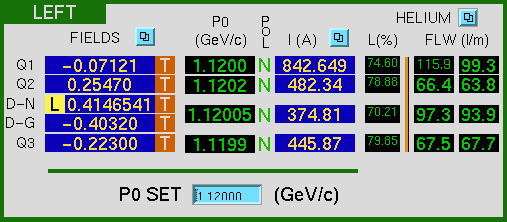
\includegraphics[angle=0,width=0.8\textwidth]{medm_halla_tools_1_cut1}
{\linespread{1.}
\caption[HRS: Magnets control]{A part of ``Hall A General Tools'' screen, 
        used for HRS (left) magnets control.}
\label{fig:hrs_mag_cntrl}}
\end{center}
\end{figure}

This box displays a brief summary of the status of the spectrometer
magnets and their cryogenic systems. The blue fields (with white
numbers) give readbacks of the magnetic fields and currents in each
magnet. The black fields also give readbacks, however in this case if
the text appears green those parameters are OK while if they are red
then that parameter is out of tolerance and may indicate a fault
condition. For example if the helium level goes below a certain point
the magnet will be automatically turned off.  In some cases it may be
desirable to monitor certain critical quantities on a strip chart
(e.g. magnet settings). A strip chart tool is available for this
purpose from the bottom of the ''EOS Menu'' button in the ''MyMenu'' window.

{\bf To set the spectrometers} for a given value of central momentum
(P0) type the desired P0 value into the light blue P0 SET box and hit
return. The magnets will be automatically 
set to the correct
values. All green numbers in the P0 column indicates that the desired
field or current settings have been reached. 

{\bf Caution:} Regarding the
dipoles, in general it's a bad idea to assume that at the first
instant that the P0 display turns green that the desired field has
been reached and you can start taking data. Stable field is in general
not achieved for from 15 to 30 minutes after reaching the nominal
desired field. This settling time depends on the magnet (the right dipole is
slower than the left dipole) and the magnitude of the field change (small
changes settle faster than big changes). Experimenters are advised to
observe both the field reading and current reading on the magnet in
question and verify that things are stable to their satisfaction
before proceeding.
 
\subsection{Powering Up Dipole Magnets:}

Use these instructions to recover from loss of a magnet due to a fault
(e.g. He level or lead flow fault). The order of actions matters. \\
(Contact Tech-On-Call if anything behaves funny or things don't
respond as expected. Sometimes after a trip an access to the Hall is
required to reset things).

\begin{list}{\arabic{enumi}.~}{\usecounter{enumi}\setlength{\itemsep}{-0.15cm}}
   \item Wait for Iout=0 (you can't and don't want to do anything while the magnet is in emergency fast dump mode.)
   \item While waiting, make a log entry re the fault. Give details such as time, coincident activities, and nature of the fault.
   \item Make sure the fault is cleared. (e.g. He level and flow rates returned to normal values and stable)
   \item In the HRS Right (Left) Dipole Systems' control panel:
   \begin{list}{}{\setlength{\itemsep}{-0.15cm}}
      \item[(a)] Press RESET (verify that all faults are cleared in the middle column)
      \item[(b)] Press ON (Display will indicate Power Supply ON and Magnet ENGAGED)
   \end{list}
\end{list}


Power supply and magnet are ready to go. From here you can return 
to "Autopilot Mode" (see Section \ref{sec:hrs-mag-set}).

\subsection{Starting Q1 Power Supply:}

 Do this when a fault causes the power supply to shut off.
 Wait for fault to clear (watch He levels). 
\begin{list}{\arabic{enumi}.~}{\usecounter{enumi}\setlength{\itemsep}{-0.15cm}}
   \item Push POWER OFF/RESET (check all faults cleared)
   \item Select desired polarity
   \item Push POWER ON
   \item Type in Setpoint (Amps) (light blue field) or re-enter P0 in Autopilot Mode.
\end{list}

\subsection{Starting Q2/3 Power Supply:}

 Do this when a fault causes the power supply to shut off.
 Wait for cause of fault to clear (watch He levels). 
 \begin{list}{\arabic{enumi}.~}{\usecounter{enumi}\setlength{\itemsep}{-0.15cm}}
   \item Push RESET 
   \item Select desired polarity
   \item Push ON
   \item Type in Current Set (light blue field) or re-enter P0 in Autopilot Mode.
\end{list}

} %infolev

\subsection{Rotation}
%
% Thanks to John LeRose for Rotation text. 07NOV2013
%
Moving an HRS
Since each HRS weighs in excess of 1,000 tons it is very important that all safety
precautions are carefully adhered to. The good news is they move very slowly (a few degrees/min
maximum), BUT 1,000 tons moving even very slowly is hard to stop. 

Hazards include:
\begin{itemize}
\item{Knocking items over.}
\item{The wheels crushing things (including fingers and toes) on the floor in the path of the 
spectrometer}
\item{Damaging the beamline or other equipment on the floor if one goes to too small 
or too large an angle, or if it just gets pushed around inadvertantly.}
\item{Tearing out of cables etc. physically attached to the superstructure}
\end{itemize}

Hazard mitigations:
\begin{itemize}
\item{Guards on either side of the wheels prevent items from getting under them.}
\item{Large pins in the floor to stop the spectrometer rotated beyond the needed angular range.}
\item{Blinking lights on the spectrometers indicating they are in motion or that motion
is possible (controls engaged etc.)}
\item{During a running experiment the run coordinator and work coordinator should know in advance 
of any moves.  Moves at any other time must be cleared with the Hall work coordinator 
before implementation.}
\item{Careful inspection of the intended path to make sure it is clear. This is part of
the pre-run checklist performed by the technical staff prior to closing the Hall and
a remote camera allows shift worker to inspect the area.}
%
%\item{Any motion that takes a spectrometer inside 14 degrees or outside x degrees
%(x being specified in the pre-run checklist and noted on the whiteboard during a run) 
%must be supervised by a trained Hall A technician.}
\end{itemize}

\infolevone{
Remote Procedure for a shift worker:
\begin{itemize}
\item{Make sure the move is part of the approved runplan (if in doubt, check with the 
run coordinator).}
\item{Check that the pre-run checklist has been completed and note and comply with any 
possible limitations to spectrometer motion (if there is a conflict inform the Run
Coordinator and do not initiate any move until the conflict is cleared).}
\item{Visually inspect the Hall using the closed circuit TV cameras to verify that there
are no obstructions.}
\item{If people are in the Hall wait until they leave (during a Controlled Access MCC keeps
track of people in the Hall). (Maybe we could soften this to "Inform EVERYONE in the Hall of
the move".)}
\item{Activate the spectrometer motion controls (see the Wiki and below) and 
move to the desired angle.}
\item{Deactivate the controls (brakes on, power off, etc.)}
\item{Update the spectrometer position information on the Hall A Controls screen}
\item{Make a halog entry indicating you've moved the spectrometer including from what angle 
to what new angle.}
\end{itemize}

Procedure for a non-run associated move in the Hall:
\begin{itemize}
\item{Inform the work coordinator of the planned move}
\item{Perform a careful visual inspection to verify that the path is clear}
\item{Check to make sure there are no temporary connections to the spectrometer (wires etc.)
that could be damaged during the move.}
\item{Inform everyone in the Hall of the move and check with them re 3.}
\item{Activate the spectrometer motion controls (see the Wiki and below) verify 
that the warning lights are on and move to the desired angle.}
\item{Deactivate the controls (brakes on, power off, etc.).}
\end{itemize}

The full proceedure for moving the spectrometer follows and can also be found on the Hall A wiki.

On hacsbc2, click the red "tool box" icon on the linux taskbar, as above. Choose 
bogies\_SetSpec so that you can determine the angle and vernier setting for the spectrometer.
Enter the spectrometer (L or R), and the angle, and you will get two options for the floor 
mark and the vernier. Generally choose the vernier closer to zero. Center the cameras on the 
desire vernier using the Move+/Move- buttons on the Hall A General Tools screen. The TV monitors 
for these cameras are on the middle shelf, in rack CH01A05.

Choose bogies\_Left (or bogies\_Right) in the tool box to bring up the bogies control screen. 
Click PSM enable and wait a few seconds for PSM OK to read YES. 
Click DM enable and wait a few seconds for DM OK to read YES.
Make sure the velocity is set to 0 and the direction is CW or CCW as desired. Click on Brake Release 
and wait for Brakes OK to read YES.

Click on ClampRelease, set the velocity to 700. Once you see the spectrometer start to move in the 
floor angle camera - you cannot see the spectrometer move in the Hall overview camera, as it only 
moves a few degrees per minute at maximum speed. For the left arm, to move to a larger angle, the 
direction should be CCW, while for the right arm CW moves the spectrometer to larger angle. The 
direction of the spectrometer is reversed by using a negative rpm. Watch the spectrometer motion 
on the cameras. When you are getting close to the desired angle, slow down to about 300 rpm. 
To stop, click on the Clamp Release button and the Brake button. Disable DM and PSM, and disconnect 
to close the GUI. Read off the floor angle mark and vernier, and input the values into the appropriate 
fields in the Alignment section of the Hall A General Tools GUI. 
}









\newpage
\section[Field Monitoring]{Field Monitoring
\footnote{
  $CVS~revision~ $Id: nmr-1999.tex,v 1.4 2003/12/17 03:59:48 gen Exp $ $ 
}
\footnote{Authors: J.LeRose \email{lerose@jlab.org}}
}

The field-monitoring controls are available using the main 
HRS screen%
\infolevtwo{ (see Figure~\ref{fig:hrs_mag_cntrl})%
}. % infolev
The dipoles' field is measured using NMR Teslameters and
field probes.

\infolevone{ 
 
\subsection{ Dipole Field Monitoring Electron Arm}

\noindent {\bf Basic Setup}

Each spectrometer dipole magnet is equipped with a Metrolab PT 4025 
NMR Teslameter, several field probes, and multiplexers (to allow switching 
between the probes).  Details of the operation and theory of operation 
for the Teslameter can be found in its user manual, 
a copy of which is available in the the counting house.
The basic layout is shown in Figure~\ref{fig:nmrbasic}


\begin{figure}
\begin{center}
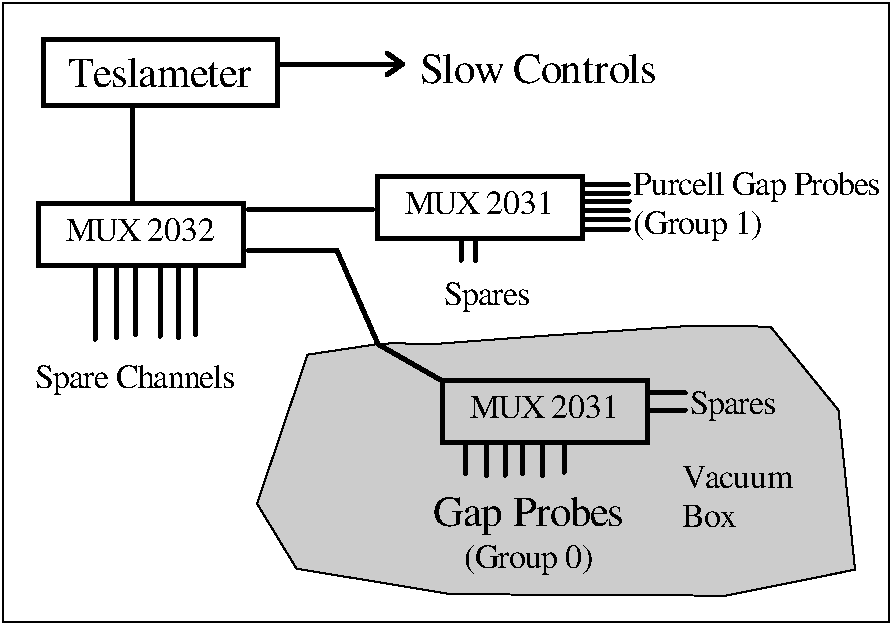
\includegraphics[angle=0,width=15cm,clip]{lerose_fig1}
{\linespread{1.}
\caption[Spectrometers: NMR System Layout]{Basic layout of NMR system}
\label{fig:nmrbasic}}
\end{center}
\end{figure}


 The "Gap Probes" (Group 0 in the controls) are located in two groups 
of three; one group on the low field side of the gap and the other on the high 
field side of the gap.  The groups of three are made up of one each of 
the manufacturer's type 3, 4 \& 5 probes, designed to cover different 
field ranges (see Table \ref{nmr_range}).  The six ``Purcell Gap Probes'' (Group 1 in 
the controls) are located in the Purcell gap of the magnet 
and consists of two each of the above types. {\em Note: Since
the fall of 1998 the multiplexer-multiplexer in both arms,
MUX 2032, has been removed and hence the ``Purcell Gap Probes'' are currently
unavailable. There are no plans to re-install this multiplexer.}

 The "Gap Probes" are equipped with coils which provide a field 
gradient that cancels out the field gradient of the magnet in the vicinity of 
the probe.  These gradient compensating coils are part of a simple circuit 
that is completely independent of the Teslameter.  The basic circuit for 
the compensating coils is shown in Figure~\ref{fig:nmrcir}


\begin{figure}
\begin{center}
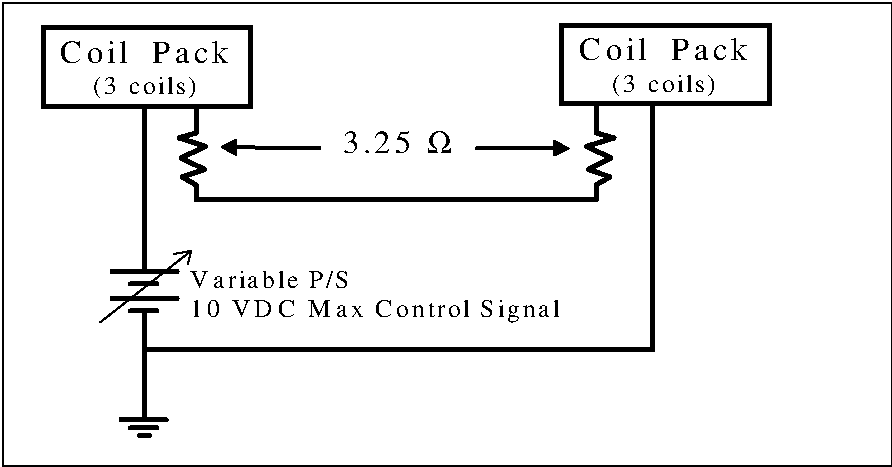
\includegraphics[angle=0,width=10cm,clip]{lerose_fig2}
{\linespread{1.}
\caption[Spectrometers: NMR Gradient Compensation]{Gradient Compensating Circuit.}
\label{fig:nmrcir}}
\end{center}
\end{figure}


%\snfig{figs/lerose_figcce.eps}{Control Voltage calibration for
%Electron Dipole }{nmrcomp4}{5in}

\begin{figure}
\begin{center}
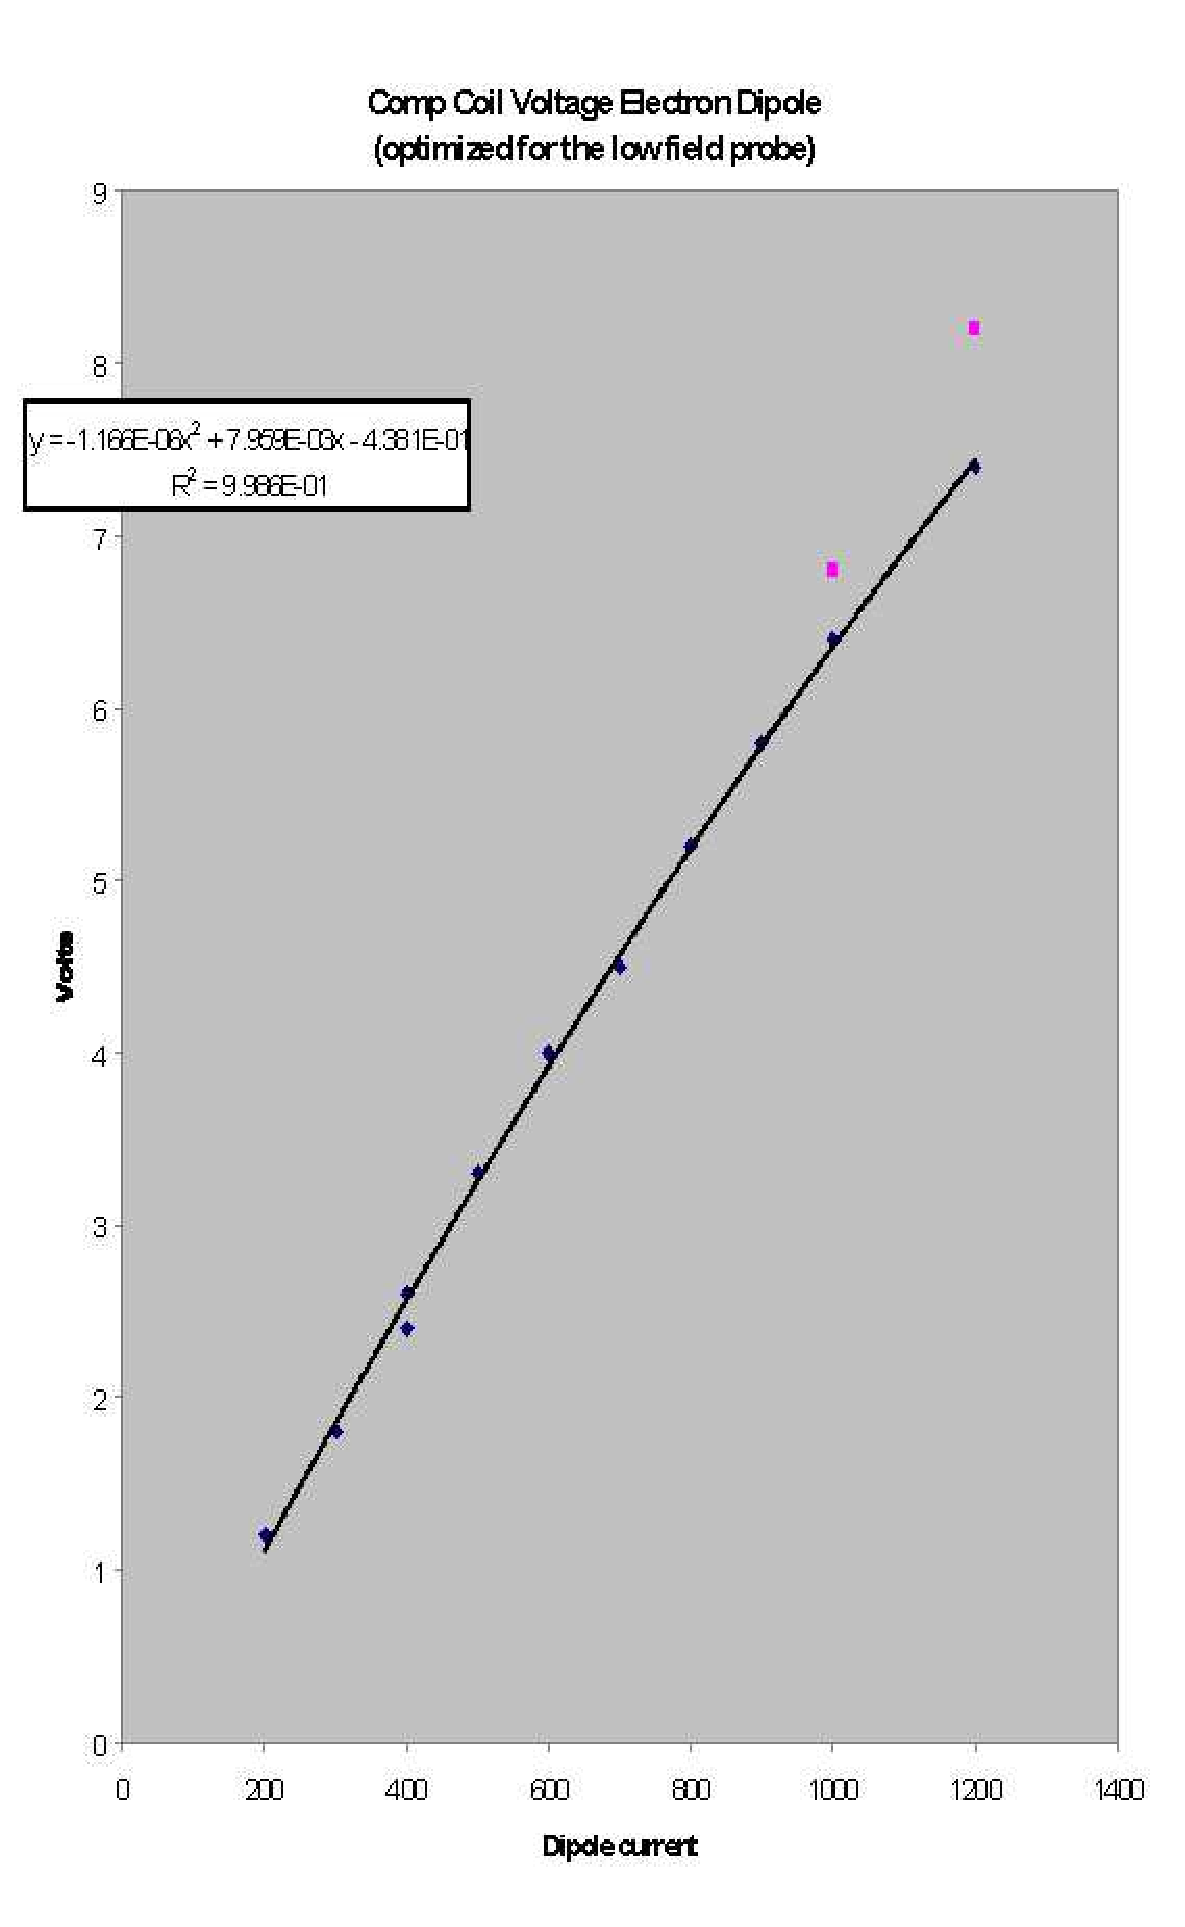
\includegraphics[angle=0,height=20cm,clip]{lerose_figcce}
{\linespread{1.}
\caption[Spectrometers: Control Voltage Calibration for Left Dipole]{Control Voltage calibration for the Left Dipole.}
\label{fig:nmrcomp4}}
\end{center}
\end{figure}

%\snfig{figs/lerose_figcch.eps}{Control Voltage calibration for
%Hadron Dipole }{nmrcomp5}{5in}
\begin{figure}
\begin{center}
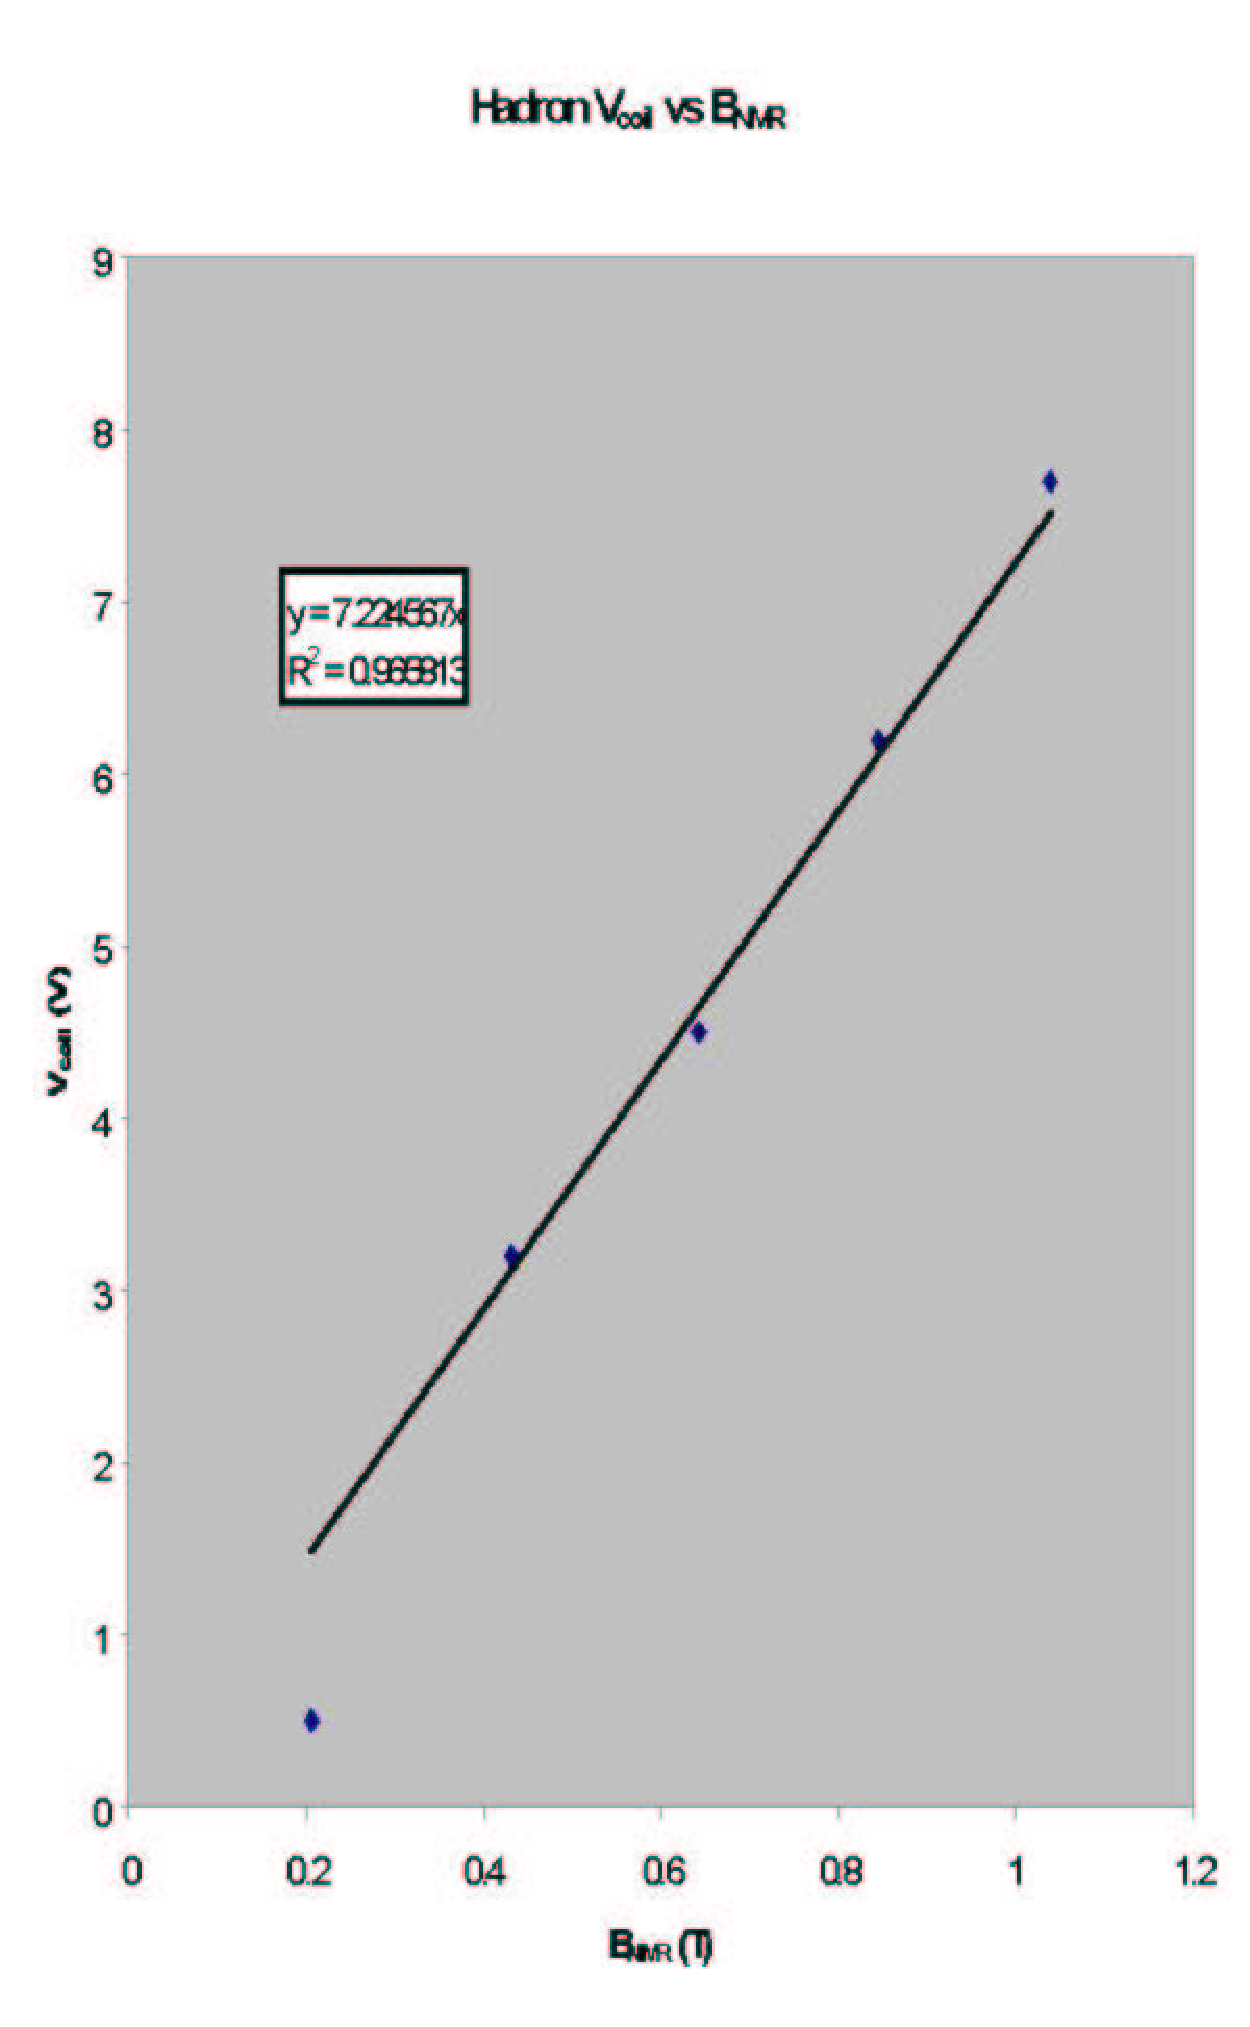
\includegraphics[angle=0,height=20cm,clip]{lerose_figcch}
{\linespread{1.}
\caption[Spectrometers: Control Voltage Calibration for Right Dipole] {Control Voltage calibration for the Right Dipole.}
\label{fig:nmrcomp5}}
\end{center}
\end{figure}

%\snfig{./figs/lerose_fig7.eps}{DAC Calibration for manual operation of NMR probes}{nmr_dac}{9in}
\begin{figure}
\begin{center}
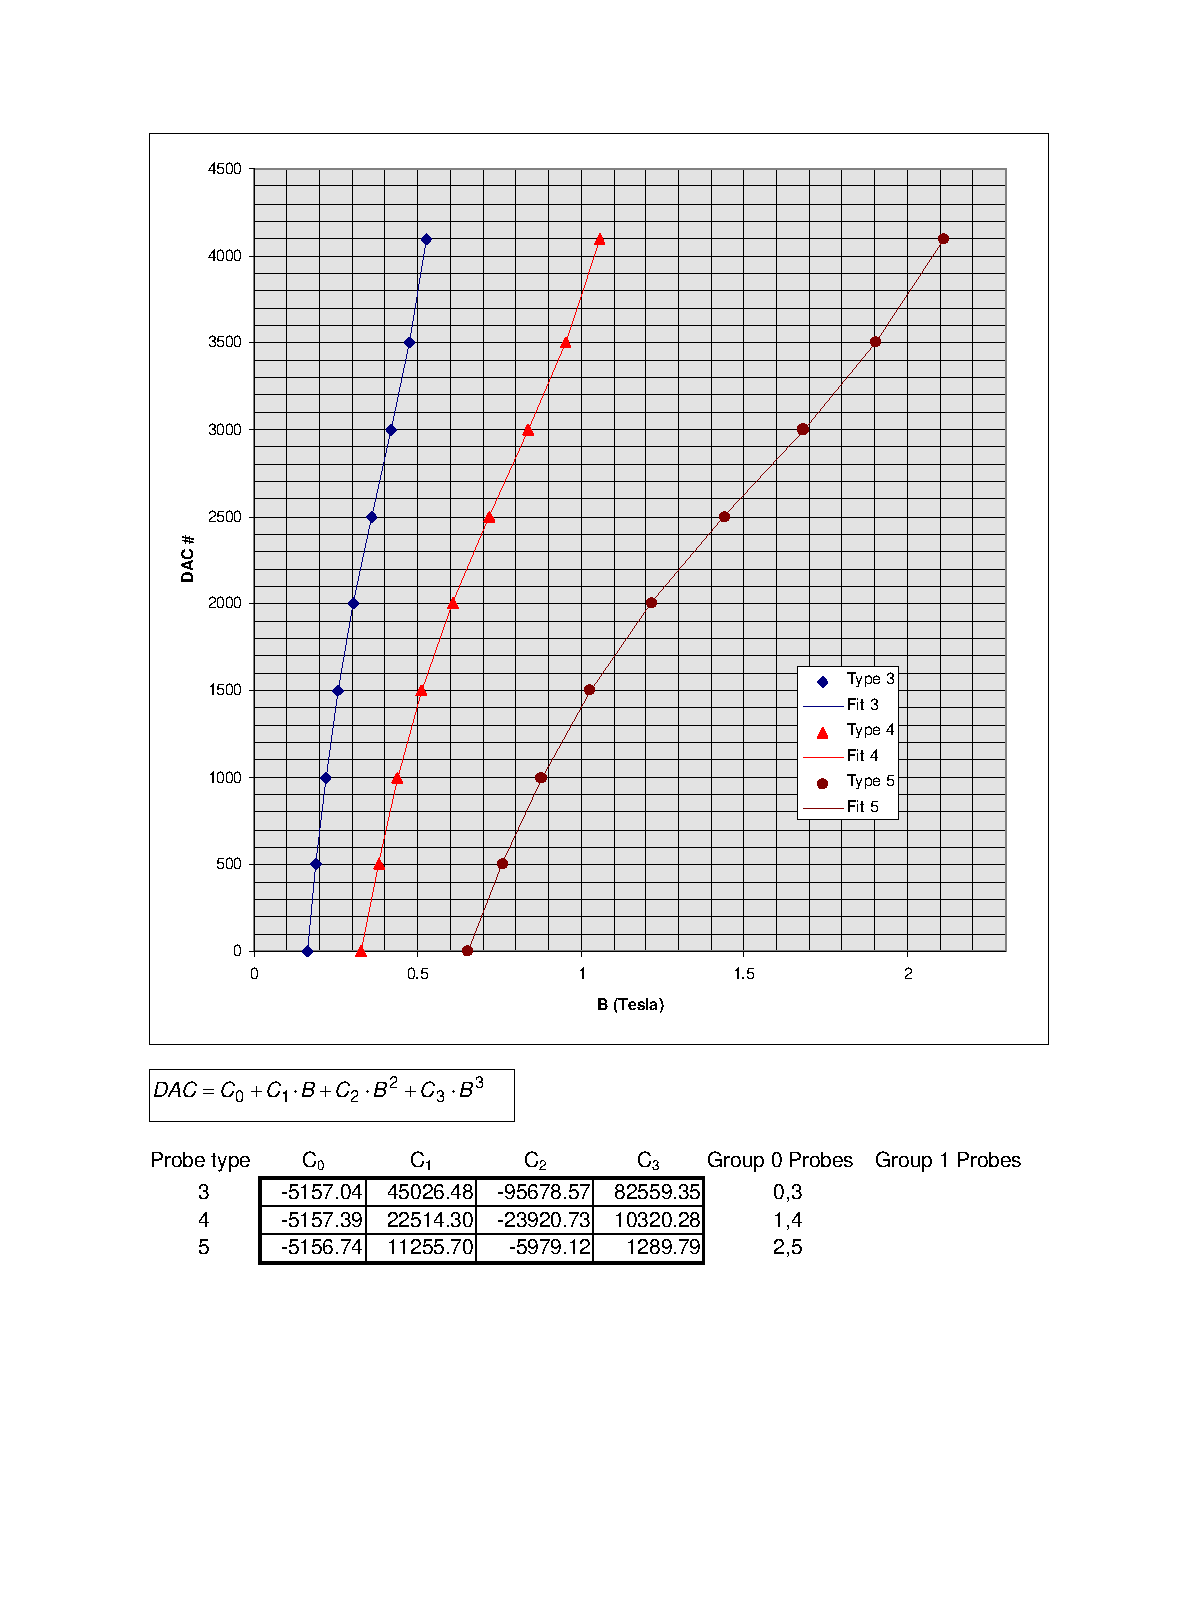
\includegraphics[angle=0,height=20cm,clip]{lerose_fig7}
{\linespread{1.}
\caption[Spectrometers: NMR Probe DAC Calibration]{DAC Calibration for manual operation of NMR probes.}
\label{fig:nmr_dac}}
\end{center}
\end{figure}

The following graphs (see Figures~\ref{fig:nmrcomp4} 
and ~\ref{fig:nmrcomp5}),can be used to determine optimum values for the 
compensating coil control voltage.  It should be noted that the setting 
of the compensating coil current is not very critical in most cases.  In 
general if you're within 10\% of the correct value everything should 
work fine.



\begin{table}
\begin{center}
\begin{tabular}{|cc|} \hline
Probe Type & Field Range (T) \\ \hline 
3 & 0.17 - 0.52 \\
4 & 0.35 - 1.05 \\
5 & 0.70 - 2.10 \\ \hline
\end{tabular}
\caption[Spectrometers: Dipole NMR Probe Field Ranges]{Dipole NMR probe field ranges}
\label{nmr_range}
\end{center}
\end{table}

} %infolev

\infolevtwo{
\subsection{NMR Operating Procedure}

When running in Autopilot mode (see: Simple Spectrometer Field Setting) the 
compensating coil voltage is set automatically and the probe appropriate for 
the field desired is selected. The gaussmeter is placed in SEARCH Mode and the 
dipole power supply software regulator is turned on. In this case the dipole current is 
adjusted to achieve the desired field. The user should just stand 
back and let it work. What follows are instructions for using
the NMR gaussmeter in situations where Autopilot doesn't work or
some special supplemental measurements are required. 

 In principle it is possible to make the field measurements using the 
SEARCH mode in the Teslameter.  In this mode you select a probe and the 
meter explores the whole field range of the probe until it finds and 
"locks" on the resonant signal indicating that it has a field 
measurement.  A ``lock" is indicated on the controls display by an ``L'' to 
the left of the field values.  This has the advantage of simplicity but in practice can 
be time consuming and doesn't always work.  The problem being, in 
situations where there is a lot of noise mixed in with the signal, the 
circuitry has problems distinguishing the signal from the noise and gets 
lost before it ever finds a lock.  The problem is exacerbated when the 
field being measured is at the high end of the probe's range.  In this 
case the search starts at the low end and keeps getting hung up on the 
noise and never gets to the field range of interest.  The solution to 
this problem is to tell the device approximately what field it's looking 
for and use the AUTO mode to find the lock.  In the procedure below that 
is what we will be doing.

In any case, for ``gap probes" (group 0) you must energize and adjust 
the gradient compensating coils for the field ranges to be measured before 
trying to make a measurement.

For studies involving 
10\% changes in the field settings the compensating coil current can be 
set once and left alone.


\noindent\underline{\bf Recommended Procedure:}(turn the {\bf SOFTWARE REGULATOR OFF} for all 
non-autopilot field measurements)\\
For group 0 probes set compensating coils appropriately (see figures).\\
Put the meter in MANUAL mode with SEARCH OFF \\
Select a probe \underline{\bf and} polarity (\underline{\bf Group 0:  
Probes 0, 1, 2 negative; Probes 3, 4, 5 positive}) \\
Type in the appropriate DAC number for the field range being measured (see below) \\
Select AUTO and wait for a lock (indicating a valid field reading) \\
Verify that you have a good lock by checking the oscilloscope for a 
clear resonant signal. \\
If you have problems see the table listing problems and possible 
solutions.

\noindent\underline{\bf Selecting DAC Number}

In selecting the DAC number to use for the field of interest use 
either the graph in Figure~\ref{fig:nmr_dac} or the polynomial at the bottom of the same figure.

\pagebreak
\noindent{\bf Problems and Solutions}\\
\begin{table}[htb]
\begin{tabular}{|p{0.4\textwidth}|p{0.55\textwidth}|}\hline
Symptom & Diagnosis and Cure \\ \hline\hline
Weird numbers on displays, controls for all magnets fouled up 
& Need to reboot.  See instructions below. \\ \hline
NMR Teslameter does not respond to commands and display shows all zeros. 
& Meter's communications are somehow hung up. Push {\bf RESET}. \\ \hline
%Will not lock & Very high noise level makes resonance hard to find. \\
%Still 
Will not lock 
& Very high noise level makes resonance hard to find. Search for the resonance manually by 
  adjusting the DAC in manual mode until you see the resonant signal.  (It helps if you know 
  what field you expect so you'll know where to look). \\ \hline
You find resonance manually but still can't get a lock 
& Check probe polarity. Try decreasing and increasing DAC number by 1. Optimize signal 
  by adjusting compensating coils. \\ \hline
Can't find resonance manually 
& Try a different probe.  Use readings from other probes to tell you where to look for 
 the resonance with the probe that's giving you trouble.  Make sure
 compensating coils are energized properly.  Make sure magnet is on. \\ \hline\hline
\end{tabular}
\caption[NMR: Problems and solutions]{NMR: Problems and solutions}
\label{tab:nmr-problems-solutions}
\end{table}

\begin{table}[ht]
\begin{center}
\begin{tabular}{|p{0.3\textwidth}|p{0.3\textwidth}|p{0.3\textwidth}|}\hline
Problems & Explanation & Action \\ \hline
NMR not locked but current is changing in the right direction 
& Normal operation for large field changes  
& Wait. (see above) \\ \hline
NMR locked but current going in the wrong direction.
& Normal operation. 
& Wait. \\ \hline
NMR locked but field not correct and current not changing 
& Field regulation is disabled or software is confused.
& Check that field regulation is enabled. Enter desired field value or one
  very near the desired value again. \\ \hline
NMR field display freezes. (Usually but not always shows  -\#.0000000)
& NMR Gaussmeter is not communicating with software.
& Push {\bf RESET}. \\ \hline
\end{tabular}
\end{center}
\caption[NMR troubleshhoting]{NMR troubleshooting
}
\label{tab:hrs_nmr_2}
\end{table}

} %infolev

\begin{safetyen}{10}{15}
\subsection{Authorized Personnel}
\end{safetyen}

The individuals shown in Table \ref{tab:nmr:personnel} are responsible for NMR operation problems.

\begin{namestab}{tab:nmr:personnel}{NMR: authorized personnel}{%
      NMR: authorized personnel.}
  \JavierGomez{\em Contact}
  \JohnLeRose{}
\end{namestab}



\newpage
\section[Collimators and Sieve Slits]{Collimators and Sieve Slits
\footnote{
  $CVS~revision~ $Id: slit.tex,v 1.5 2003/12/13 06:23:38 gen Exp $ $ 
}
\footnote{Authors: J.LeRose \email{lerose@jlab.org}}
}

Both spectrometers have front-end devices for calibrating the optical
properties of the spectrometers. These are known as the collimator boxes.
These boxes are positioned between the scattering chamber and the 
first quadrupoles (Q1). Each box is carefully aligned and rigidly attached
to the  entrance flange of the Q1 of the respective spectrometer.  The boxes are
part of the vacuum system of the spectrometer.
In the septum configuration sieve slits and collimators are installed and removed manually.

Inside each box a ladder is mounted which is guided by a linear bearing
and moved up and down by a ball screw. On this ladder 3 positions are 
available to insert collimators. Below this ladder
a special valve is mounted that can isolate the vacuum in the spectrometer
from the target system. This valve should be activated when it is moved
in front of the holes connecting the box with spectrometer and target chamber.
\infolevone{
A schematic view of the collimator box is shown in Fig.~\ref{fig:coll}.

\begin{figure}
\begin{center}
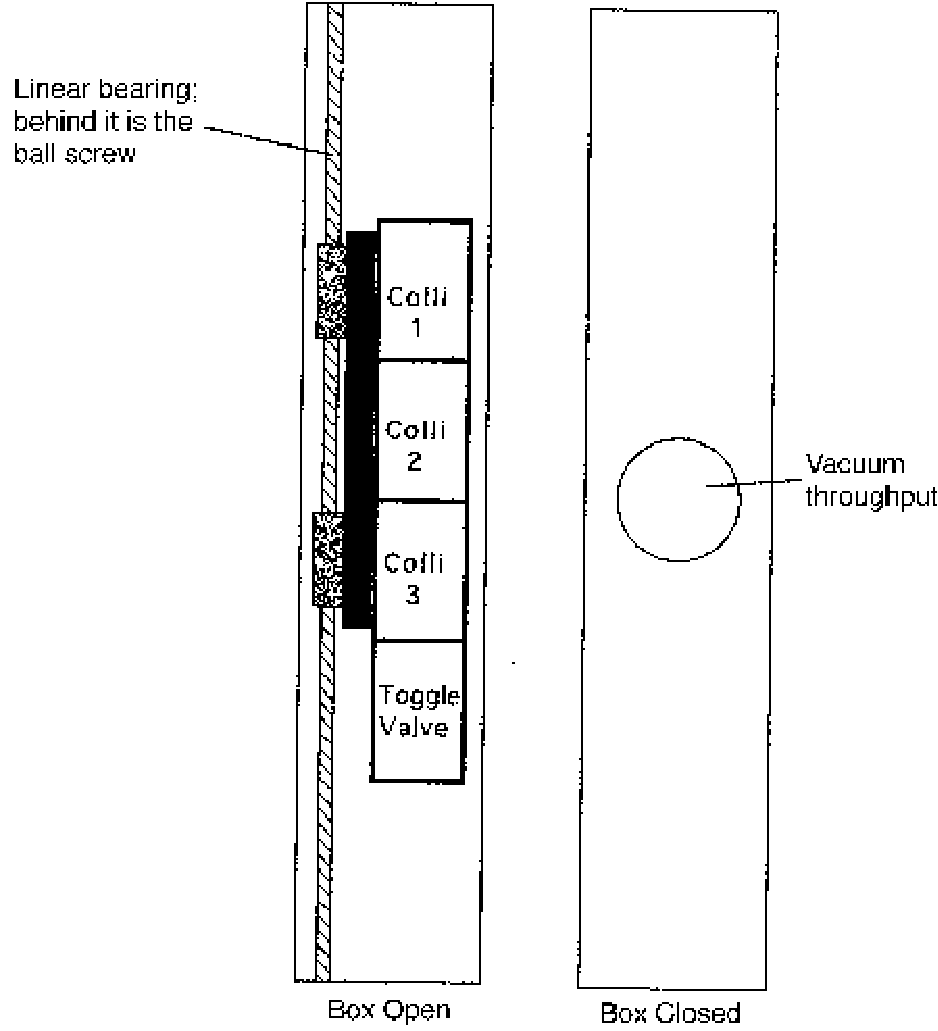
\includegraphics[angle=0,width=13cm,clip]{collimator_clip}
{\linespread{1.}
\caption[Spectrometers: Collimator Box Schematic]{Schematic layout of the collimator box.}
\label{fig:coll}}
\end{center}
\end{figure}
} %infolev

Vacuum requirement is $10^{-6}$ Torr. The material for the box is 
aluminum. It is possible to open one side of the box so that
collimators can be exchanged. The
reproducibility of collimator positions after moving
the ladder and/or after replacing a collimator is
better than 0.1 mm in horizontal and vertical direction.
The dimensions of the box are
roughly height=175 cm , width=35 cm and depth=15 cm.
The tolerance in the dimension
of the 7 msr collimator hole is $\pm0.5$ mm in each direction. 
The tolerance in the position
of each of the sieve-slit holes is $\pm0.1$ mm in each direction.

\infolevone{
\begin{figure}
\begin{center}
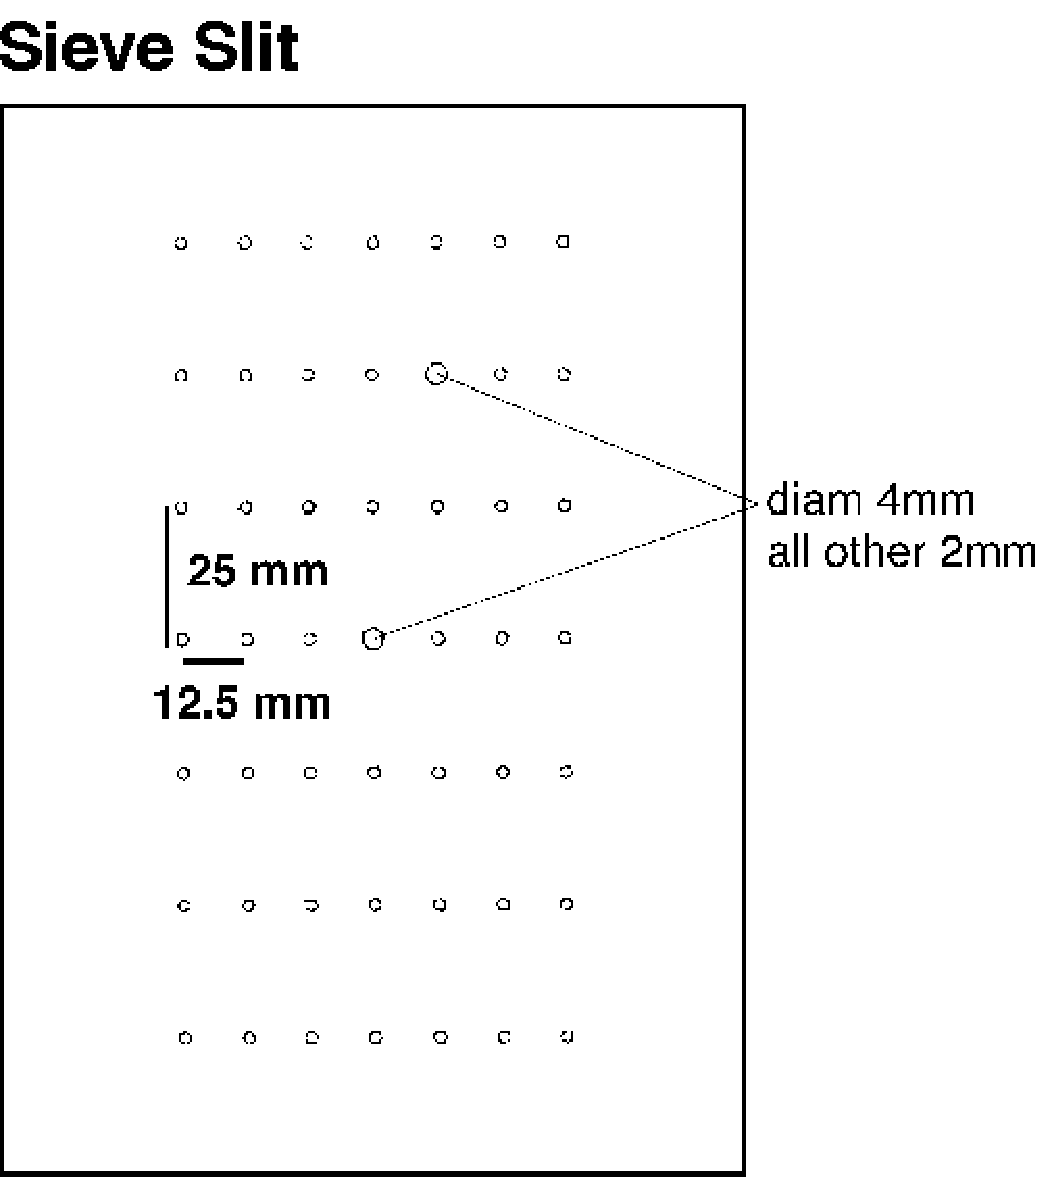
\includegraphics[angle=0,width=13cm,clip]{sieveslit}
{\linespread{1.}
\caption[Spectrometers: Sieve Slit]{Sieve slit collimator for optics calibration.}
\label{fig:sieve}}
\end{center}
\end{figure}
} %infolev
A typical sieve slit collimator 
\infolevone{(shown in Fig.~\ref{fig:sieve})
} %infolev 
consists of a plate of roughly 14 cm x 20 cm containing 49 holes
positioned in a regular 7x7 pattern. This slit is made out of 5
mm thick tungsten.
The holes have a diameter of 2 mm except for the central one and one positioned
off-diagonal which have a diameter of 4 mm. The horizontal distance between the
holes is 12.5 mm while the vertical distance is 25.0 mm.
%
%To get the latest information on the dimensions and locations of the collimators see 
%the Hall A homepage on the web%
%\htmladdnormallinkfoot{}{\url{
%http://hallaweb.jlab.org/
%}}.

To get the latest information on the dimensions and locations of the collimators see 
the Hall A homepage on the web%
\htmladdnormallinkfoot{}{\url{
http://hallaweb.jlab.org/
}}.

\begin{safetyen}{10}{15}
\subsection{Safety Assessment}

The collimator boxes form part of the vacuum system for each spectrometer. All hazards
identified in section spectrometer vacuum section applies to the collimator box as well.

In addition, safe access to the top of
the collimator boxes is needed  during manual operation of the box as outlined below.
Due to the proximity of the collimator boxes to the scattering chamber, and Q1 quadrupoles,
all necessary safety precautions with regards to vacuum windows, electrical power cables, 
cryogenic transfer lines, and high magnetic field should be taken. The same precautions also apply 
to the collimators and sieves in the septum configuration. In that case the sieve and collomators
can be considered part of the beamline. A survey and
appropriate RADCON designated proceedures must be followed when dealing with septum sieves 
and collimators.
\end{safetyen}

\infolevtwo{
\subsection{Operating Procedure}
Slit position is changed remotely from the standard Hall A control screen.
In the case of a spectrometer configuration involving the septum magnets collimators and sieves are
changed manually in the Hall.
} %infolev

\subsection{Authorized  Personnel} 

\begin{itemize} 
\item[~]E. Folts - x7857 (mechanical and vacuum systems).
\item[~]J. Gomez - x7498 (computer controls and electrical systems).
\end{itemize} 

% ===========  CVS info
% $Header: /group/halla/analysis/cvs/tex/osp/src/hrs/slit.tex,v 1.5 2003/12/13 06:23:38 gen Exp $
% $Id: slit.tex,v 1.5 2003/12/13 06:23:38 gen Exp $
% $Author: gen $
% $Date: 2003/12/13 06:23:38 $
% $Name:  $
% $Locker:  $
% $Log: slit.tex,v $
% Revision 1.5  2003/12/13 06:23:38  gen
% Septum added. Name tables. Polishing
%
% Revision 1.4  2003/12/05 06:49:07  gen
% infolevels added, polishing
%
% Revision 1.3  2003/06/06 16:13:37  gen
% Revision printout changed
%
% Revision 1.2  2003/06/05 23:30:00  gen
% Revision ID is printed in TeX
%
% Revision 1.1.1.1  2003/06/05 17:28:31  gen
% Imported from /home/gen/tex/OSP
%
%  Revision parameters to appear on the output

\newpage
\infolevtwo{
\section[Spectrometer Alignment]{Spectrometer Alignment
\footnote{
  $CVS~revision~ $Id: AlignmentOps.tex,v 1.8 2003/12/17 03:59:48 gen Exp $ $ 
}
\footnote{Authors: J.Gomez \email{gomez@jlab.org}}
}

At present, the systems implemented to determine the alignment of each spectrometer
(roll, vertical angle/pointing and horizontal angle/pointing) without the help of the
Accelerator Division Survey group are limited to roll, vertical angle and horizontal angle.
All alignment information is displayed in the ``ALIGNMENT'' mosaic of the ``Hall A
General Tools'' EDM screen%
\infolevtwo{ (see Fig.~\ref{fig:medm-hlamain-tools})}
(``EOS Menu'' $-->$ ``EDM (HLA Main)'' $-->$ ``Hall A Main Menu'' $-->$ ``Tools'').

A bi-axial inclinometer is used to determine the roll and vertical angle (also known as pitch)
of each spectrometer. These inclinometers are attached to the back of the dipoles at the power
supply platform level. The raw inclinometer measurements, in Volts,
are displayed as ``Tilt X'' and ``Tilt Y''. The inclinometer temperature is also given
(`` Tilt T''), in degree Celsius. From these values, the ``ROLL'' and ``PITCH'' values are
calculated.
Agreement between the inclinometer readings and survey measurements
are better than $\pm$ 0.1 mrad over all presently available history.

The horizontal spectrometer angle is determined from floor marks set in
place by the survey group. Floor marks have been placed every 0.5 $^\circ$ covering the useful range of
both spectrometers.
There are two concentric rings of floor marks in the hall. We will concentrate in the
inner ring which covers the angular range of both spectrometers. The outer ring is
similar.
The inner-ring floor marks are located at a distance of $\sim$10 $m$ from the target center.
A ruler attached to each spectrometer dipole runs over the floor marks and it acts as a vernier to interpolate
between marks. The location of a given floor mark on the ruler can be viewed from the Hall A Counting
House through a TV camera (labeled ``Front Camera'') .
The camera is able to move along the length of the ruler so that any
parallax effect can be eliminated. The camera motion is controlled from the ``Tools'' screen
through two push buttons (``FRONT CAMERA'' - ``MOVE +'' and ``MOVE --'').
Two fields in the ``ALIGNMENT'' mosaic
(``Flr Mrk'' and ``Vernier'') allow to input
the values read from the TV monitor. The effective spectrometer angle is then calculated and displayed
as ``Angle''. The application ``HRS Floor Marks'' calculates the floor mark and vernier value
to which the spectrometer should be set
to obtain a given angle. Spectrometer horizontal angle surveys and floor mark determinations
agree to $\pm$ 0.2 mrad.

\newpage
\begin{safetyen}{10}{15}
\subsection{Authorized  Personnel} 
\end{safetyen}
The authorized personnel is shown in table \ref{tab:align:personnel}.
\begin{namestab}{tab:align:personnel}{HRS alignment: authorized personnel}{%
      HRS alignment: authorized personnel.}
  \JessieButler{\em Contact}
\end{namestab}

} %infolev


% ===========  CVS info
% $Header: /group/halla/analysis/cvs/tex/osp/src/hrs/all.tex,v 1.3 2003/06/06 15:44:08 gen Exp $
% $Id: all.tex,v 1.3 2003/06/06 15:44:08 gen Exp $
% $Author: gen $
% $Date: 2003/06/06 15:44:08 $
% $Name:  $
% $Locker:  $
% $Log: all.tex,v $
% Revision 1.3  2003/06/06 15:44:08  gen
% Revision printout changed
%
% Revision 1.2  2003/06/05 23:30:00  gen
% Revision ID is printed in TeX
%
% Revision 1.1.1.1  2003/06/05 17:28:31  gen
% Imported from /home/gen/tex/OSP
%
%  Revision parameters to appear on the output

%\chapter{High Resolution Spectrometers (HRS)}
\graphicspath{{hrs/figs/}}
\renewcommand{\dirfig}[0]{hrs/figs}
\renewcommand{\dircur}[0]{hrs}

\infolevone{
\chapter[High Resolution Spectrometers (HRS)]{High Resolution Spectrometers (HRS)
}
\footnote{Authors: J.LeRose \email{lerose@jlab.org}}
}
\label{chap:hrs}

\infolevone{
\section{Overview}
   
The Hall A spectrometers and associated instrumentation are designed to 
perform high resolution and high accuracy experiments.  The goal is to 
achieve a missing mass resolution of $\sim$ 200-500 keV to clearly 
identify the nuclear final state.  An absolute accuracy of $\sim$ 1\% is 
also required by the physics program planned in the Hall, which implies 
$\sim$ 10$^{-4}$ accuracy in the determination of particle momenta and 
$\sim$ 0.1 mr in the knowledge of the scattering angle.

The instruments needed are a high resolution electron spectrometer 
(HRES) and a high resolution hadron spectrometer (HRHS), both with a 
large angular and momentum acceptance.

\begin{figure}[tbp]
\begin{center}
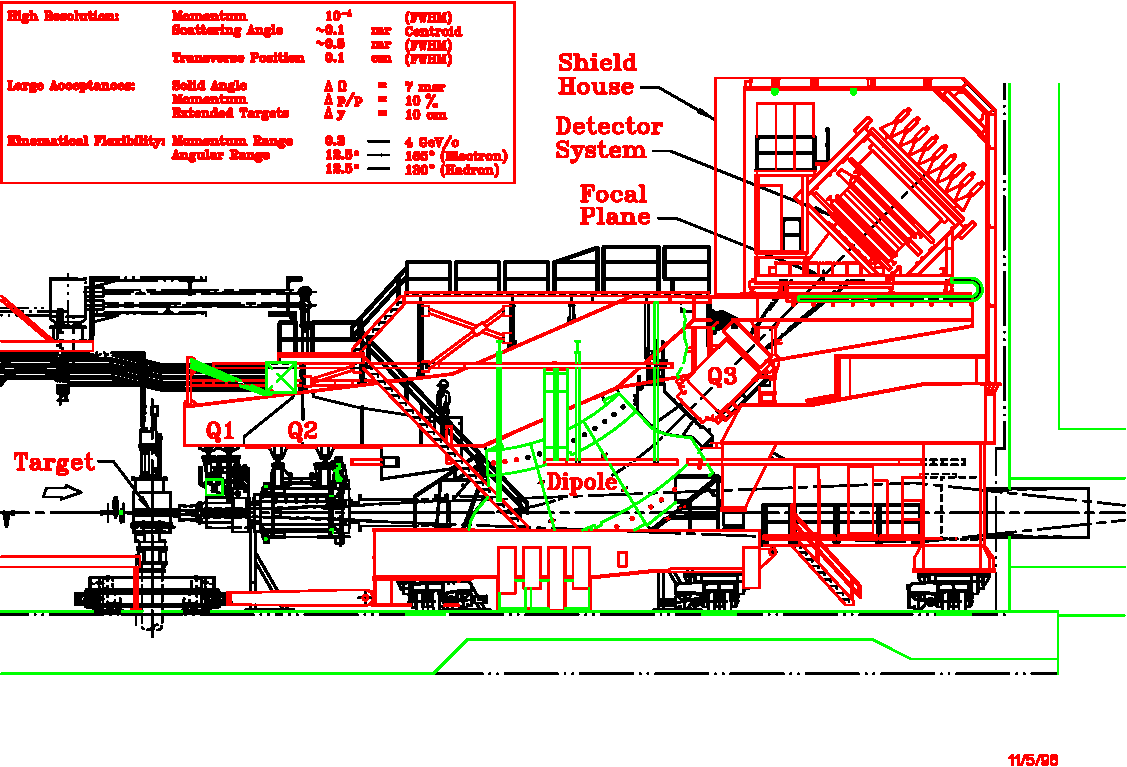
\includegraphics[angle=0,width=0.9\textwidth,clip]{figure0101_r}
\caption[Spectrometers: Elevation View of Hall~A HRS]{A side view of the Hall~A
HRS spectrometer.}  
\label{fig:hrs_ev}
\end{center}
\end{figure}
 
\begin{figure}[tbp]
\begin{center}
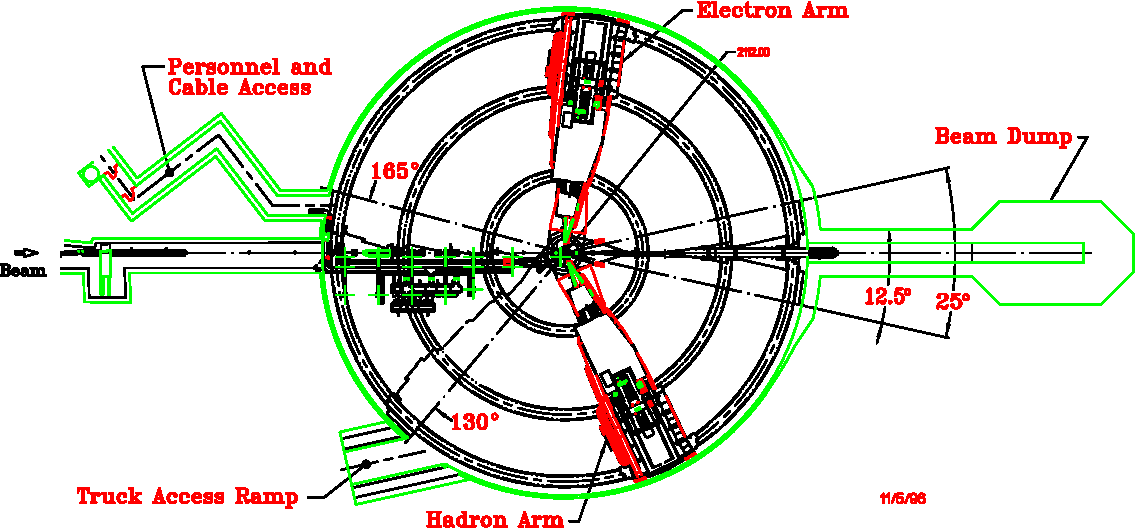
\includegraphics[angle=0,width=0.9\textwidth,clip]{figure0102_r}
\caption[Spectrometers: Plan View of Hall~A]{A bird's eye view of the Hall~A
end-station at TJNAF.}  
\label{fig:hrs_pv}
\end{center}
\end{figure}


A layout of the 4 GeV/c High Resolution Electron Spectrometer is shown 
on Figures~\ref{fig:hrs_pv} and \ref{fig:hrs_ev}.
Its main design characteristics are 
given in the attached table.  The spectrometer has a vertical bending 
plane and 45$^{\circ}$ bending angle.  The QQDQ design includes four 
independent superconducting magnets, three current-dominated 
cos2$\theta $ quadrupoles and one iron-dominated dipole with 
superconducting racetrack coils.  The second and third quadrupoles of 
each spectrometer have sufficiently similar field requirements that they 
are of identical design and construction.  The overall optical length, 
from target to focal plane, is 23.4 m.  Optically, the HRHS 
is essentially identical to HRES. In fact the two spectrometers can be used 
interchangeably to detect either positively or negatively charged particles 
as needed by any particular experiment. They are now commonly refered to 
as ``The Left Arm'' and ``The Right Arms'' rather than ``Hadron'' and ``Electron'' 

The support structure includes all system elements which bear the weight 
of the various spectrometer components and preserve their spatial 
relationship as required for 45$^{\circ}$ vertical bending optics.

The alignment and positioning system includes all the elements which 
measure and adjust the spatial relationship.  The support structure 
consists of the fabricated steel components which support the magnets, 
detector, shield house and associated equipment.  It is composed of the 
box beam, which supports the outer elements in fixed relative position 
atop the dipole; the dipole support bracket, upon which the dipole rests on 
the jacks; the cradle, upon which the dipole rests through the vertical 
positioning system, VPS; and a portion of the shield house load through 
the inboard legs of the gantry; the gantry, which supports the shield 
house and the magnet power supplies; and the bogies, which support the 
cradle-gantry assembly and roll on the floor plates and provide the 
driving power to move the two spectrometer arms.

The detector package (described in detail in Chapter \ref{chap:hrs-det})
is supported on the box beam and is surrounded by 
the shield house.  It must perform two functions, tracking and particle 
identification, PID.  The most important capability of focusing 
spectrometers is measuring precisely the momenta and entrance 
orientations of the tracks.  Momentum resolution of 10$^{-4}$ is 
obtainable, consistent with the resolution of the incident beam.

The actual configuration of the detector package varies from experiment to
experiment. The description given here is only an example of what is possible.
}

\infolevone{
A particle traversing the detector stack 
(Figure~\ref{fig:hrs_electron_det}) encounters two sets of horizontally
mounted, vertical drift wire chambers (x,y) with two planes of 368
wires in each chamber. The track resolution is $\sim$ 100 $\mu$m.  
From the chamber information both 
positions and angles in the dispersive and transverse directions can be 
determined.  The information from these chambers is the principal input 
of the tracking algorithms.

The chambers are followed by a scintillator hodoscope plane designated S1. 
This plastic scintillator array provides the timing reference for 
the drift chambers, and is also used in trigger formation and in combination 
with a second hodoscope pair it can provide time of flight particle 
identification.  These scintillators can also be used to perform crude 
tracking.

The next element encountered by a particle is a gas threshold \Cherenkov{} 
detector.  This is used for particle identification.  This gas threshold \Cherenkov{} detector can be swapped 
against an Aerogel detector, with a similar function.

The second hodoscope plane, S2, is located directly behind the 
gas \Cherenkov{}.  Its function is essentially the same as that of S1.  
In the hadron spectrometer an option exists to have this hodoscope 
pair be preceded by a third chamber, to improve tracking.
 Each of the two spectrometers 
have gas and Aerogel \Cherenkov{} detectors which can be used
 when they are in electron detection mode.

The final elements in the detector stack on HRSE are 
the pre-shower and the total-absorber lead glass shower 
calorimeter.  This is used for energy determination and PID.

\begin{figure}[tbp]
\begin{center}
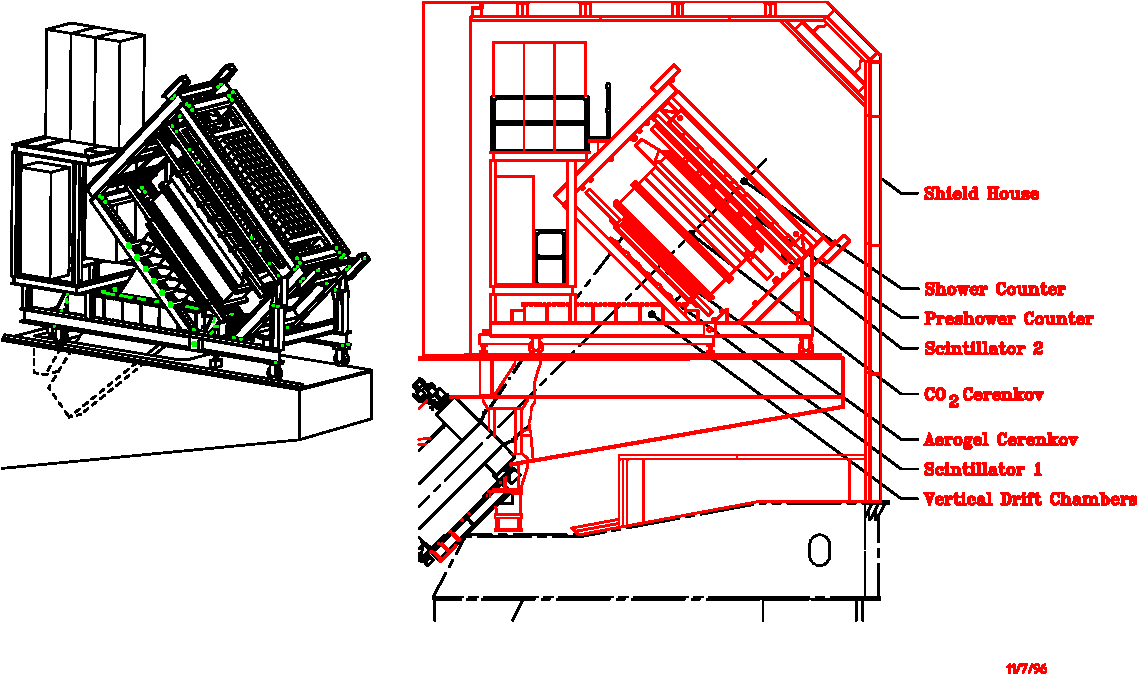
\includegraphics[angle=0,width=\textwidth,clip]{figure0103_r}
{\linespread{1.}
\caption[Spectrometers: Electron Arm Detectors]{The electron spectrometer detector stack.}
\label{fig:hrs_electron_det}}
\end{center}
\end{figure}

\begin{figure}[tbp]
\begin{center}
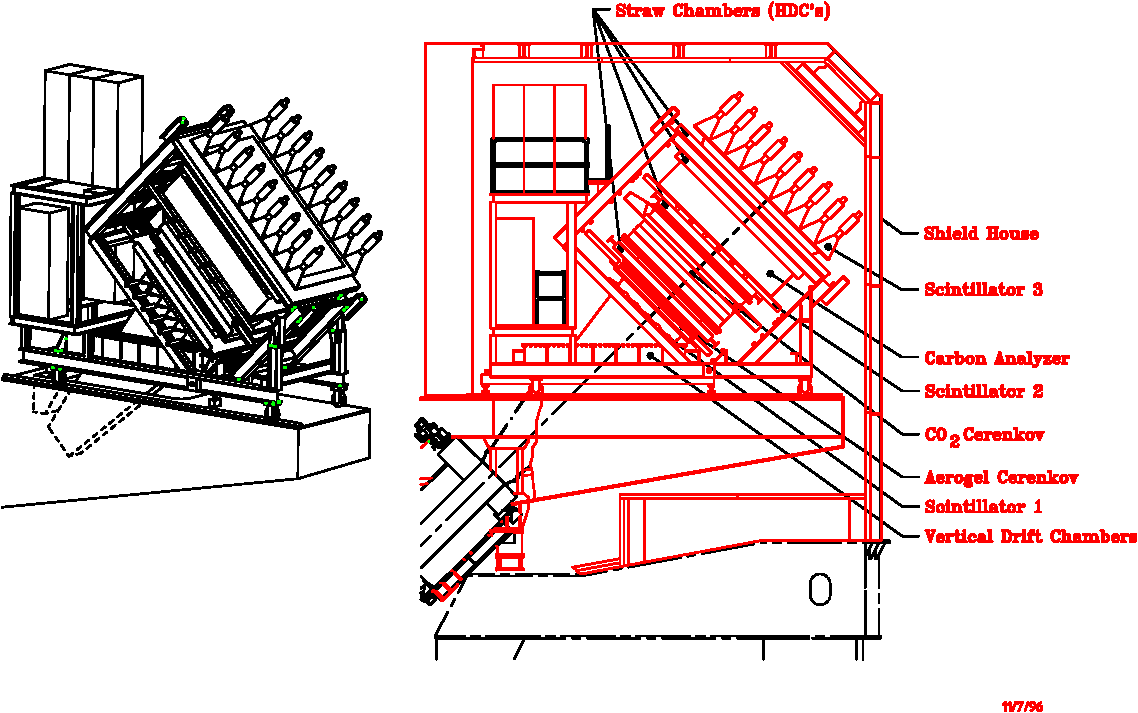
\includegraphics[angle=0,width=\textwidth,clip]{figure0104_r}
{\linespread{1.}
\caption[Spectrometers: Hadron Arm Detectors]{The hadron spectrometer detector stack.}
\label{fig:hrs_hadron_det}}
\end{center}
\end{figure}


The hadron detector is shown schematically in 
Figure~\ref{fig:hrs_hadron_det}.  It consists 
of two sets of (x,y) vertical drift wire chambers identical to those of the 
electron arm.  The remaining part of the detection system is used to 
define the level 1 trigger, as well as for particle identification and 
timing.  It consists of two minimally segmented planes of 
scintillation counters equipped with photomultipliers at both ends, and 
it includes \Cherenkov{} counters (gas CO$_2$ and Aerogel).

In addition, a proton polarimeter is installed in the back of the 
detector package to measure the polarization of the proton using a 
segmented carbon analyzer up to 60 cm in thickness to allow measurements 
over a wide range of proton energies.  A pair of front and a pair of 
rear straw tube wire chambers determine the incident and 
scattered angles, respectively.  The 
polarimeter detectors are dimensioned to accept a 20$^{\circ}$ cone of 
scattered protons.

Several support systems are necessary in addition to the basic 
components mentioned above.  They include gas supply systems for the 
wire chambers, high voltage supplies, readout electronics, a second 
level trigger, software for data analysis and testing, and a remotely 
controllable mechanical system.

For each spectrometer, all detectors are mounted on a 
single rigid support frame along with their associated electronics.  The trigger electronics are located on the support frame, next to the detectors.

To reduce the resolution degrading effects of multiple scattering, the 
entire interior of the spectrometer from the collimator box to the detector hut 
is a vacuum vessel.  The ends of this evacuated volume are capped by 
relatively thin vacuum windows.
}

\begin{safetyen}{0}{0}
\section{High Resolution Spectrometers}
\label{sec:hrs-safety}
\end{safetyen}

The principle concern with the spectrometers is that they are large, 
and have associated vacuum, hydraulic, cryogenic and magnet systems all of 
which can be potentially dangerous.

The bogies which move the massive 1200 ton spectrometers must be 
carefully operated.  Inspection of the floor and wheels to ensure there is no 
debris which the wheels could ride over is mandatory.  Similarly 
personnel need to be aware that the spectrometers are moving so that no one 
inadvertently gets trapped.

The vacuum systems associated with the spectrometers are essentially 
pressure vessels (see Chapter \ref{chap:vacuum} for more details).
Care should be exercised so as not to puncture the 
windows.

The magnets themselves are installed inside cryostats.  These vessels 
are exposed to high pressures and are therefore equipped with safety 
relief valves and burst discs.

The hydraulic system originally intended to operate the vertical positioning system (VPS) 
and the horizontal positioning system (HPS) has effectively been dismantled, after problems were encountered during the initial attempted operation of the system.

The cryogenic system operates at elevated pressure at 4K.  One must 
guard against cold burns and take the normal precautions with pressure 
vessels when operating this system.  Only authorized personnel are permitted to install 
and take out U tubes.

The magnets have a great deal of stored energy as they are large 
inductors. Always make sure people are clear of them and that
the dump resistor is attached to the magnet.

There are several major safety concerns with regards to the detectors, 
namely 1) flammable gas located in the VDC, 2) ODH hazard due to 
CO$_2$ in the \Cherenkov{} counter, 3) high voltage due to the photo 
multipliers on the various detectors and 4) a thin vacuum window 
separating the detector array from the vacuum system in the 
spectrometers.

\infolevltone{
\begin{safetyen}{5}{10}
For more information consult the full OSP manual~\cite{HallAosp}.
\end{safetyen}
} %infolev

\begin{safetyen}{10}{15}
\subsection{Authorized Personnel}
\end{safetyen}

In the event that problems arise during 
operation of the magnets, qualified personnel should be notified
(see Table \ref{tab:hrs:personnel}).  
This includes any prolonged or serious problem with the source of magnet 
cryogens (the ESR).  On weekends and after hours there will be a 
designated individual on call for magnet services.  Any member of the 
Hall A technical staff is qualified to deal with unusual magnet 
situations but in the event of serious problems the technician on
call should be contacted.

\begin{namestab}{tab:hrs:personnel}{HRS: authorized personnel}{%
      HRS: authorized personnel. ''W.B'' stands for the white board 
      in the counting house.}
   \TechonCall{\em Contact}
   \EdFolts{}
   \JackSegal{}
   \HeidiFansler{}
   \JessieButler{}
   \AndrewLumanog{}
   \JasonGlorioso{}
   \MahlonLong{}
\end{namestab}

\infolevone{
\section{The Magnets of HRS}

Each HRS is composed of three superconducting quadrupole magnets, Q1, Q2, 
and Q3, and one superconducting dipole magnet.  The large quadrupoles were 
manufactured for JLab by SIEMENS, the small quadrupole by SACLAY, while 
the dipole was built for JLab by WANG NMR.  The quadrupole magnets are 
referred to as Q1, Q2, and Q3, where a particle first traverses Q1, then 
Q2 and the dipole magnet and finally traverses Q3.

The magnet system is followed by a large steel and concrete detector 
hut, in which all detector elements reside.  Most of the 
detector elements have been built by universities involved in the Hall A 
physics program.

The HRS magnet system is the cornerstone of the Hall A activities.  
Many of the experiments approved in Hall A center on physics at high 
resolution and other short-range phenomena, and rely on a spectrometer 
able to momentum analyze charged particles up to very high momenta.  The 
design value for the maximum momentum accessible to the HRS magnet 
system is 4 GeV/c.
}

\subsection{Magnets and Power Supplies}

\infolevone{
The HRS magnet's are all superconducting and hence their coils must be 
maintained at cryogenic temperatures during operations.  The LHe 
required by the magnets is supplied by the End Station Refrigerator, ESR.

All the HRS magnets cryogenic services are supplied through the overhead 
cryogenic lines.  The distribution network begins at the distribution 
box over the pivot.  This box is connected to the rest of the network 
via the flexible transfer lines over the pivot.  The network is adjacent 
to the upstairs catwalk of the HRS.

Cryogenic information about each magnet is available on the control 
screens in the counting house, one for each magnet.  Normally during run 
periods the control screens are sent upstairs to the Hall A counting 
house and information on all the HRS magnets is available on the HRS 
control screen located in the center of the main console.  The control 
of all magnets is described in a following Section.

The power supplies for the magnets are located on the gantry balcony 
adjacent to the magnets.  The supplies are all cooled with low conductivity water (LCW).
}

\begin{safetyen}{10}{15}

Under no 
circumstances should any panel of any magnet power supply be opened by someone 
other than authorized personnel.  There are also 
signs posted listing the dangers of high magnetic fields.
\end{safetyen}

\infolevone{
A control interface for the power supplies is available through the 
HRS control screen in the Hall A counting house.
}

\infolevone{
\subsection{Quadrupole Magnets}

The quadrupoles provide some of the 
focusing properties of the spectrometer and to a large extent 
its acceptance.  Operating limits imposed on the 
quads are as follows: 1850A for Q2 and Q3 and 3250A 
for Q1.

All three quadrupoles for the HRS spectrometer are warm iron 
superconducting magnets.  The soft iron around the superconducting coil 
enhances the field at the coil center and reduces stray fields.  The 
basic parameters for the first quadrupole, Q1, are an effective length of about 
0.9 $m$, useful aperture of 0.3 $m$ and a field gradient of 9.5 
T/m.  To achieve the lowest possible angle setting of the HRS 
spectrometer (with respect to the beam line) the incident electron beam passes through
a notch in the outer yoke of Q1 when the spectrometer is at
its smallest angle of 12.5$^\circ$ . The 
other two quadrupoles, Q2 and Q3, are essentially identical with an 
effective (magnetic) length of about 1.8 meter, a useful aperture of 
0.6 $m$ and a field gradient of 3.5 T/m.
}

\infolevthree{
The maximum operating currents (assuming a 4 GeV/c momentum particle) 
for the quadrupoles are about 3000 A, 1700 A, and 1600 A, for Q1, Q2, and 
Q3, respectively.  This will render pole field values 
of 1.2, 1.0, and 1.0 T, respectively.  The energy stored in the 
quadrupole fields is sufficient to cause an unrecoverable quench if all 
the energy stored is dumped into the magnets.  Therefore a quench 
protection circuit is incorporated.  However, a quench can only happen 
if the cryomagnets have a helium level below the coil 60\% during operation.

The operating current to the Q1 quadrupole coils is provided by Danfysik 
System 8000 power supplies, which can operate up to 3500 A current and 5 
V.  The power supplies will be cooled with a combined maximum 
water flow of 45 liters per minute.

In addition to the main quadrupole windings, all quadrupoles have 
multipole windings.  To further optimize focusing properties of the HRS 
magnet system, it was intended to operate including some of these multipole 
trim coils in order to reduce higher order aberrations.
The operating current for these multipole corrections would be 
small, only (the multipole corrections are typically less than 2\% of 
the main quadrupole field), of order 50 A. Since the sextupoles were inadvertently 
installed rotated 90 $^\circ$ from their correct
orientation, these trim coils are now considered useless 
and there are at present no plans to use them.

\subsection{Cryogenic Procedures}

The cryogenics control is handled by the JLab Cryogenics Group.  The cryo control coordinator 
can be reached at the CHL (x7405) or by calling the MCC.

\subsection{First Time Startup Check List.}  

See attached check lists for all quadrupole and dipole magnets
 (Tables~\ref{tab:dip_check}, \ref{tab:q1_check}, and \ref{tab:q23_check}).
} %infolev

\infolevone{
\subsection{Dipole Magnet}

The dipole, by virtue of its field index, provides both
dispersion and focusing.  The present operations envelope 
states that the supply for the left HRS dipole may not be
operated at a current above 1800 A (4.4 GeV/c). The supply for the right HRS
dipole may not be operated above 1200 A (3.2 GeV/c), due to complications
caused by an internal short. 

The dipole for the HRS spectrometer is a superconducting, cryostable 
magnet.  Its basic parameters are an effective length of about 6.6 $m$, a 
bend radius of 8.4 $m$, and a gap width of 25 $cm$.  It is configured to 
achieve a 45 degree bending angle for 4 GeV/c momentum particles at a 
central field excitation of 1.6 T.  For the HRS dipole to reach 1.6 T 
an operating current of about 1500 A is required.
} %infolev

\infolevthree{
The dipole has been designed to achieve cryostability up to a field of 2 
T, and this property has been extensively tested up to a field of 1.6 T. 
 The cryostable coils are equipped with an energy removal circuit to 
cover the possibility of an unrecoverable quench.  However, this can 
only happen if the helium level drops below the coil during operation.  
The current to the coils will be provided by a Dynapower Corporation power 
supply, which can operate up to 2000 A and 10 V.  This 
power supply is located on the gantry beside the dipole, and will be 
cooled with a maximum water flow of 35 liters per minute.
The total water flow needed to cool the 4 power 
supplies for the HRS magnet system (dipole and quadrupoles) amounts to 
80 liters per minute, with a supply pressure of cooling water for Hall A 
of 100 psi.
} %infolev

\infolevtwo{
\section{Operation of the HRS Magnets}

\subsection{Introduction}

This is an abbreviated operating manual for 
the HRS superconducting magnets specifically designed for Hall A 
experimenters.  It provides instructions for setting currents, invoking 
NMR field regulation and general system monitoring.  Curious readers are 
directed to the references for more in-depth operating instructions and 
other technical manuals. Copies of the following supporting
documents are available in the Hall A Control Room and through the Hall A webpage
(see Table~\ref{tab:hrs-mag-manuals}).

\begin{table}[htp]
\begin{center}
\begin{tabular}{|l|l|}
\hline
References & \\
\hline 
WANG NMR Dipole & User Manual \\
Dynapower & Instruction Manual \\
Appendix & NMR Tesla meter \\
Appendix & NMR Field Regulation \\
Siemens/Fug & Q2/Q3 Magnet Instrumentation and Power Supplies \\
Saclay/Danfysik & Q1 Power Supply Manual \\
TOSP & HRS Dipole \\
TOSP & HRS Quadrupole Q1 \\
TOSP & HRS Quadrupole Q2, Q3 \\
HRS & SC Dipole Magnet Safety Review Vol. 2 \\
HRS & SC Quad Safety Review Vol. 1 \\ \hline
\end{tabular}
\end{center}
\caption[HRS Magnets: extra manuals]{HRS Magnets: extra manuals available in 
     Hall A Control Room.}
\label{tab:hrs-mag-manuals}
\end{table}

\subsection{Simple HRS Setting (Autopilot Mode)}
\label{sec:hrs-mag-set} 

 The magnets are controlled remotely using EPICS~\cite{EPICSwww} and
 EDM~\cite{EDMwww} GUI, provided that everything is working and power 
 supplies are turned on and ready to go.
 The appropriate interface runs
 on the computer \mycomp{hacsbc2} (see Section \ref{sec:contr-ha-menu}).
 On the ``Hall A General Tools'' control screen, in the upper left, there is 
 a rectangular box for each spectrometer (see Figure~\ref{fig:hrs_mag_cntrl}). 
\begin{figure}
\begin{center}
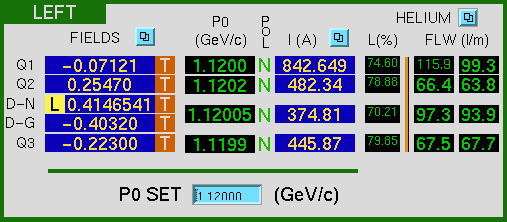
\includegraphics[angle=0,width=0.8\textwidth]{medm_halla_tools_1_cut1}
{\linespread{1.}
\caption[HRS: Magnets control]{A part of ``Hall A General Tools'' screen, 
        used for HRS (left) magnets control.}
\label{fig:hrs_mag_cntrl}}
\end{center}
\end{figure}

This box displays a brief summary of the status of the spectrometer
magnets and their cryogenic systems. The blue fields (with white
numbers) give readbacks of the magnetic fields and currents in each
magnet. The black fields also give readbacks, however in this case if
the text appears green those parameters are OK while if they are red
then that parameter is out of tolerance and may indicate a fault
condition. For example if the helium level goes below a certain point
the magnet will be automatically turned off.  In some cases it may be
desirable to monitor certain critical quantities on a strip chart
(e.g. magnet settings). A strip chart tool is available for this
purpose from the bottom of the ''EOS Menu'' button in the ''MyMenu'' window.

{\bf To set the spectrometers} for a given value of central momentum
(P0) type the desired P0 value into the light blue P0 SET box and hit
return. The magnets will be automatically 
set to the correct
values. All green numbers in the P0 column indicates that the desired
field or current settings have been reached. 

{\bf Caution:} Regarding the
dipoles, in general it's a bad idea to assume that at the first
instant that the P0 display turns green that the desired field has
been reached and you can start taking data. Stable field is in general
not achieved for from 15 to 30 minutes after reaching the nominal
desired field. This settling time depends on the magnet (the right dipole is
slower than the left dipole) and the magnitude of the field change (small
changes settle faster than big changes). Experimenters are advised to
observe both the field reading and current reading on the magnet in
question and verify that things are stable to their satisfaction
before proceeding.
 
\subsection{Powering Up Dipole Magnets:}

Use these instructions to recover from loss of a magnet due to a fault
(e.g. He level or lead flow fault). The order of actions matters. \\
(Contact Tech-On-Call if anything behaves funny or things don't
respond as expected. Sometimes after a trip an access to the Hall is
required to reset things).

\begin{list}{\arabic{enumi}.~}{\usecounter{enumi}\setlength{\itemsep}{-0.15cm}}
   \item Wait for Iout=0 (you can't and don't want to do anything while the magnet is in emergency fast dump mode.)
   \item While waiting, make a log entry re the fault. Give details such as time, coincident activities, and nature of the fault.
   \item Make sure the fault is cleared. (e.g. He level and flow rates returned to normal values and stable)
   \item In the HRS Right (Left) Dipole Systems' control panel:
   \begin{list}{}{\setlength{\itemsep}{-0.15cm}}
      \item[(a)] Press RESET (verify that all faults are cleared in the middle column)
      \item[(b)] Press ON (Display will indicate Power Supply ON and Magnet ENGAGED)
   \end{list}
\end{list}


Power supply and magnet are ready to go. From here you can return 
to "Autopilot Mode" (see Section \ref{sec:hrs-mag-set}).

\subsection{Starting Q1 Power Supply:}

 Do this when a fault causes the power supply to shut off.
 Wait for fault to clear (watch He levels). 
\begin{list}{\arabic{enumi}.~}{\usecounter{enumi}\setlength{\itemsep}{-0.15cm}}
   \item Push POWER OFF/RESET (check all faults cleared)
   \item Select desired polarity
   \item Push POWER ON
   \item Type in Setpoint (Amps) (light blue field) or re-enter P0 in Autopilot Mode.
\end{list}

\subsection{Starting Q2/3 Power Supply:}

 Do this when a fault causes the power supply to shut off.
 Wait for cause of fault to clear (watch He levels). 
 \begin{list}{\arabic{enumi}.~}{\usecounter{enumi}\setlength{\itemsep}{-0.15cm}}
   \item Push RESET 
   \item Select desired polarity
   \item Push ON
   \item Type in Current Set (light blue field) or re-enter P0 in Autopilot Mode.
\end{list}

} %infolev

\subsection{Rotation}
%
% Thanks to John LeRose for Rotation text. 07NOV2013
%
Moving an HRS
Since each HRS weighs in excess of 1,000 tons it is very important that all safety
precautions are carefully adhered to. The good news is they move very slowly (a few degrees/min
maximum), BUT 1,000 tons moving even very slowly is hard to stop. 

Hazards include:
\begin{itemize}
\item{Knocking items over.}
\item{The wheels crushing things (including fingers and toes) on the floor in the path of the 
spectrometer}
\item{Damaging the beamline or other equipment on the floor if one goes to too small 
or too large an angle, or if it just gets pushed around inadvertantly.}
\item{Tearing out of cables etc. physically attached to the superstructure}
\end{itemize}

Hazard mitigations:
\begin{itemize}
\item{Guards on either side of the wheels prevent items from getting under them.}
\item{Large pins in the floor to stop the spectrometer rotated beyond the needed angular range.}
\item{Blinking lights on the spectrometers indicating they are in motion or that motion
is possible (controls engaged etc.)}
\item{During a running experiment the run coordinator and work coordinator should know in advance 
of any moves.  Moves at any other time must be cleared with the Hall work coordinator 
before implementation.}
\item{Careful inspection of the intended path to make sure it is clear. This is part of
the pre-run checklist performed by the technical staff prior to closing the Hall and
a remote camera allows shift worker to inspect the area.}
%
%\item{Any motion that takes a spectrometer inside 14 degrees or outside x degrees
%(x being specified in the pre-run checklist and noted on the whiteboard during a run) 
%must be supervised by a trained Hall A technician.}
\end{itemize}

\infolevone{
Remote Procedure for a shift worker:
\begin{itemize}
\item{Make sure the move is part of the approved runplan (if in doubt, check with the 
run coordinator).}
\item{Check that the pre-run checklist has been completed and note and comply with any 
possible limitations to spectrometer motion (if there is a conflict inform the Run
Coordinator and do not initiate any move until the conflict is cleared).}
\item{Visually inspect the Hall using the closed circuit TV cameras to verify that there
are no obstructions.}
\item{If people are in the Hall wait until they leave (during a Controlled Access MCC keeps
track of people in the Hall). (Maybe we could soften this to "Inform EVERYONE in the Hall of
the move".)}
\item{Activate the spectrometer motion controls (see the Wiki and below) and 
move to the desired angle.}
\item{Deactivate the controls (brakes on, power off, etc.)}
\item{Update the spectrometer position information on the Hall A Controls screen}
\item{Make a halog entry indicating you've moved the spectrometer including from what angle 
to what new angle.}
\end{itemize}

Procedure for a non-run associated move in the Hall:
\begin{itemize}
\item{Inform the work coordinator of the planned move}
\item{Perform a careful visual inspection to verify that the path is clear}
\item{Check to make sure there are no temporary connections to the spectrometer (wires etc.)
that could be damaged during the move.}
\item{Inform everyone in the Hall of the move and check with them re 3.}
\item{Activate the spectrometer motion controls (see the Wiki and below) verify 
that the warning lights are on and move to the desired angle.}
\item{Deactivate the controls (brakes on, power off, etc.).}
\end{itemize}

The full proceedure for moving the spectrometer follows and can also be found on the Hall A wiki.

On hacsbc2, click the red "tool box" icon on the linux taskbar, as above. Choose 
bogies\_SetSpec so that you can determine the angle and vernier setting for the spectrometer.
Enter the spectrometer (L or R), and the angle, and you will get two options for the floor 
mark and the vernier. Generally choose the vernier closer to zero. Center the cameras on the 
desire vernier using the Move+/Move- buttons on the Hall A General Tools screen. The TV monitors 
for these cameras are on the middle shelf, in rack CH01A05.

Choose bogies\_Left (or bogies\_Right) in the tool box to bring up the bogies control screen. 
Click PSM enable and wait a few seconds for PSM OK to read YES. 
Click DM enable and wait a few seconds for DM OK to read YES.
Make sure the velocity is set to 0 and the direction is CW or CCW as desired. Click on Brake Release 
and wait for Brakes OK to read YES.

Click on ClampRelease, set the velocity to 700. Once you see the spectrometer start to move in the 
floor angle camera - you cannot see the spectrometer move in the Hall overview camera, as it only 
moves a few degrees per minute at maximum speed. For the left arm, to move to a larger angle, the 
direction should be CCW, while for the right arm CW moves the spectrometer to larger angle. The 
direction of the spectrometer is reversed by using a negative rpm. Watch the spectrometer motion 
on the cameras. When you are getting close to the desired angle, slow down to about 300 rpm. 
To stop, click on the Clamp Release button and the Brake button. Disable DM and PSM, and disconnect 
to close the GUI. Read off the floor angle mark and vernier, and input the values into the appropriate 
fields in the Alignment section of the Hall A General Tools GUI. 
}









\newpage
\section[Field Monitoring]{Field Monitoring
\footnote{
  $CVS~revision~ $Id: nmr-1999.tex,v 1.4 2003/12/17 03:59:48 gen Exp $ $ 
}
\footnote{Authors: J.LeRose \email{lerose@jlab.org}}
}

The field-monitoring controls are available using the main 
HRS screen%
\infolevtwo{ (see Figure~\ref{fig:hrs_mag_cntrl})%
}. % infolev
The dipoles' field is measured using NMR Teslameters and
field probes.

\infolevone{ 
 
\subsection{ Dipole Field Monitoring Electron Arm}

\noindent {\bf Basic Setup}

Each spectrometer dipole magnet is equipped with a Metrolab PT 4025 
NMR Teslameter, several field probes, and multiplexers (to allow switching 
between the probes).  Details of the operation and theory of operation 
for the Teslameter can be found in its user manual, 
a copy of which is available in the the counting house.
The basic layout is shown in Figure~\ref{fig:nmrbasic}


\begin{figure}
\begin{center}
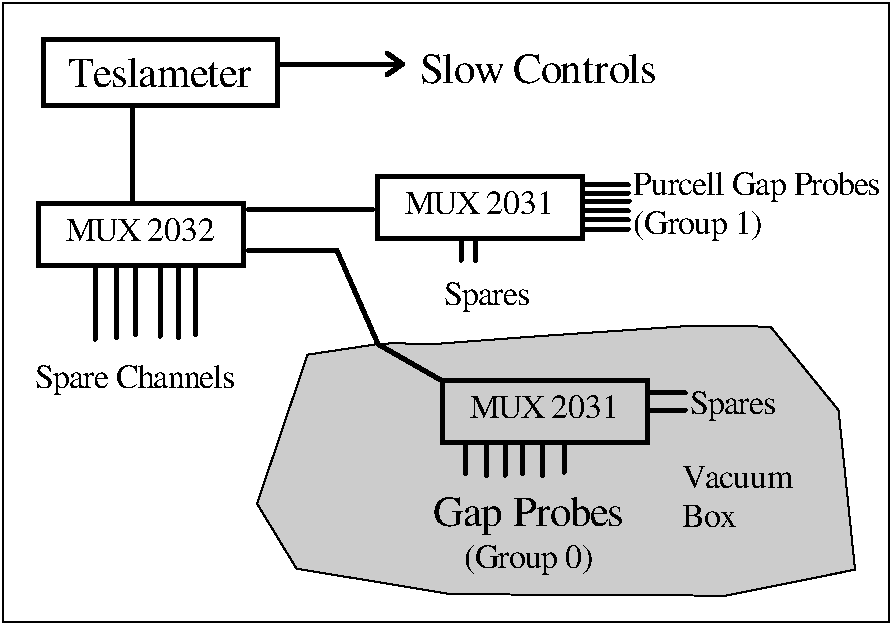
\includegraphics[angle=0,width=15cm,clip]{lerose_fig1}
{\linespread{1.}
\caption[Spectrometers: NMR System Layout]{Basic layout of NMR system}
\label{fig:nmrbasic}}
\end{center}
\end{figure}


 The "Gap Probes" (Group 0 in the controls) are located in two groups 
of three; one group on the low field side of the gap and the other on the high 
field side of the gap.  The groups of three are made up of one each of 
the manufacturer's type 3, 4 \& 5 probes, designed to cover different 
field ranges (see Table \ref{nmr_range}).  The six ``Purcell Gap Probes'' (Group 1 in 
the controls) are located in the Purcell gap of the magnet 
and consists of two each of the above types. {\em Note: Since
the fall of 1998 the multiplexer-multiplexer in both arms,
MUX 2032, has been removed and hence the ``Purcell Gap Probes'' are currently
unavailable. There are no plans to re-install this multiplexer.}

 The "Gap Probes" are equipped with coils which provide a field 
gradient that cancels out the field gradient of the magnet in the vicinity of 
the probe.  These gradient compensating coils are part of a simple circuit 
that is completely independent of the Teslameter.  The basic circuit for 
the compensating coils is shown in Figure~\ref{fig:nmrcir}


\begin{figure}
\begin{center}
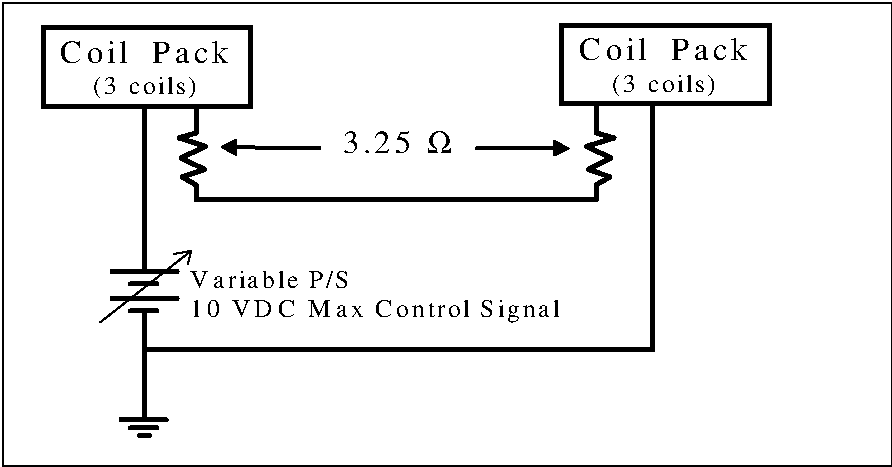
\includegraphics[angle=0,width=10cm,clip]{lerose_fig2}
{\linespread{1.}
\caption[Spectrometers: NMR Gradient Compensation]{Gradient Compensating Circuit.}
\label{fig:nmrcir}}
\end{center}
\end{figure}


%\snfig{figs/lerose_figcce.eps}{Control Voltage calibration for
%Electron Dipole }{nmrcomp4}{5in}

\begin{figure}
\begin{center}
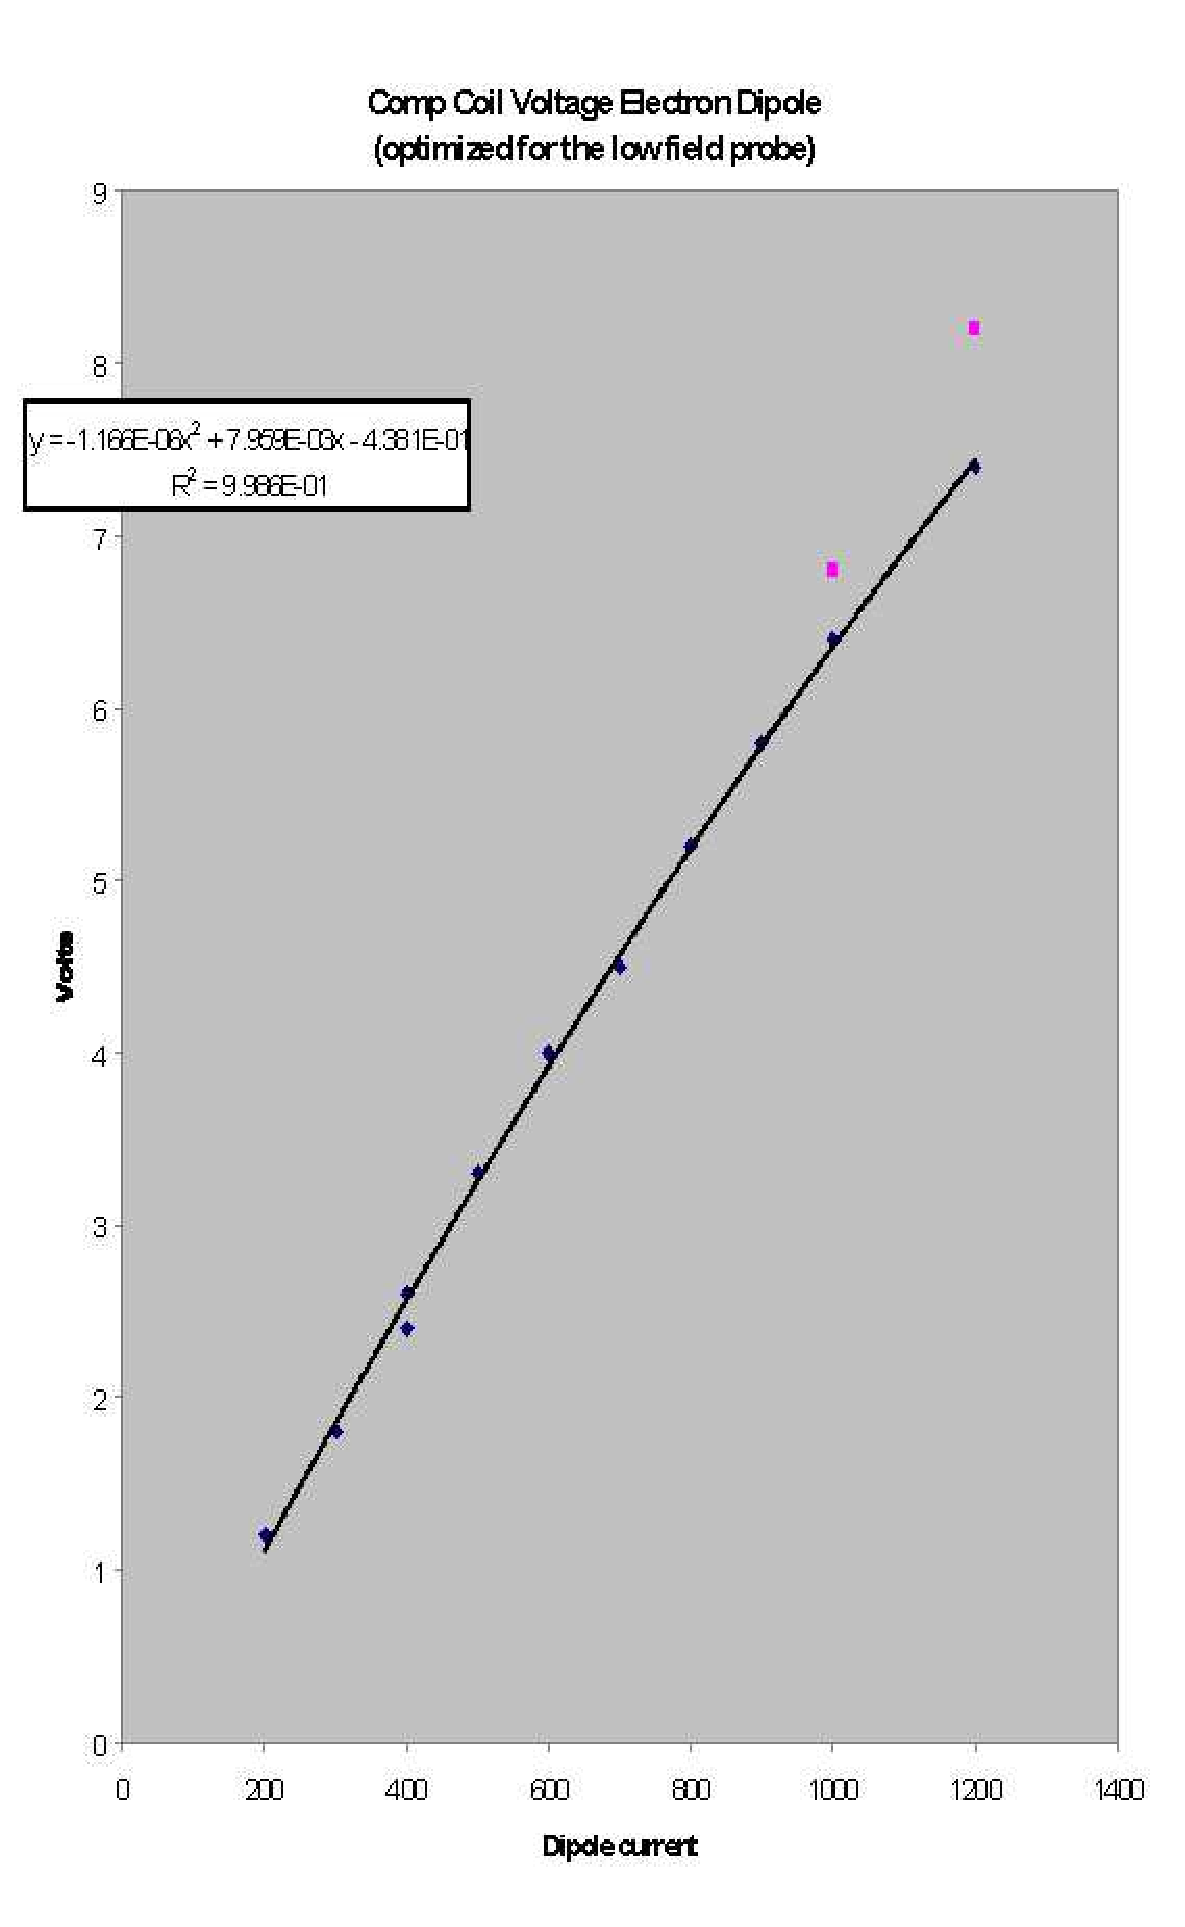
\includegraphics[angle=0,height=20cm,clip]{lerose_figcce}
{\linespread{1.}
\caption[Spectrometers: Control Voltage Calibration for Left Dipole]{Control Voltage calibration for the Left Dipole.}
\label{fig:nmrcomp4}}
\end{center}
\end{figure}

%\snfig{figs/lerose_figcch.eps}{Control Voltage calibration for
%Hadron Dipole }{nmrcomp5}{5in}
\begin{figure}
\begin{center}
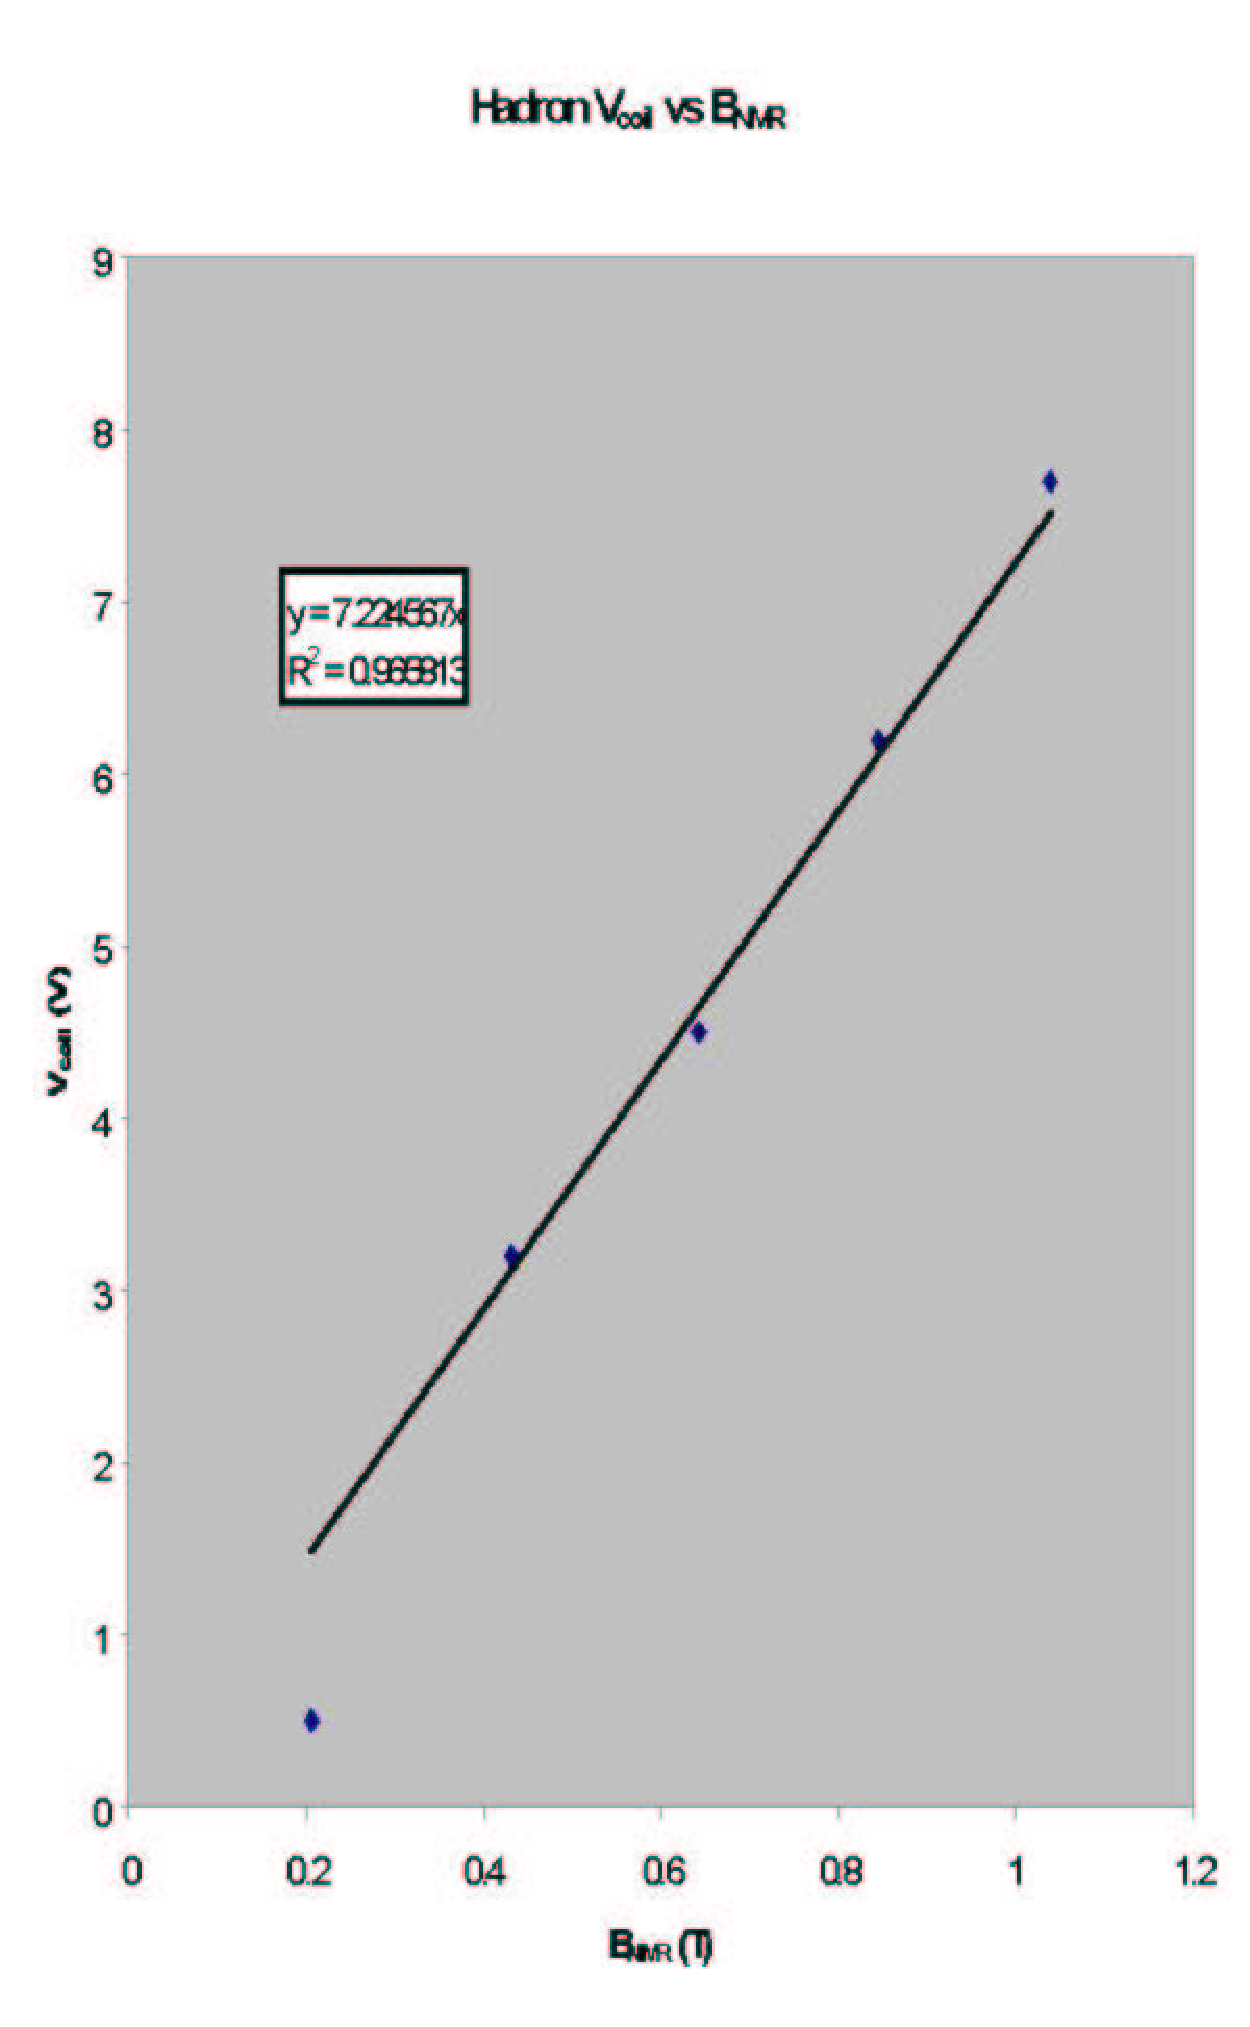
\includegraphics[angle=0,height=20cm,clip]{lerose_figcch}
{\linespread{1.}
\caption[Spectrometers: Control Voltage Calibration for Right Dipole] {Control Voltage calibration for the Right Dipole.}
\label{fig:nmrcomp5}}
\end{center}
\end{figure}

%\snfig{./figs/lerose_fig7.eps}{DAC Calibration for manual operation of NMR probes}{nmr_dac}{9in}
\begin{figure}
\begin{center}
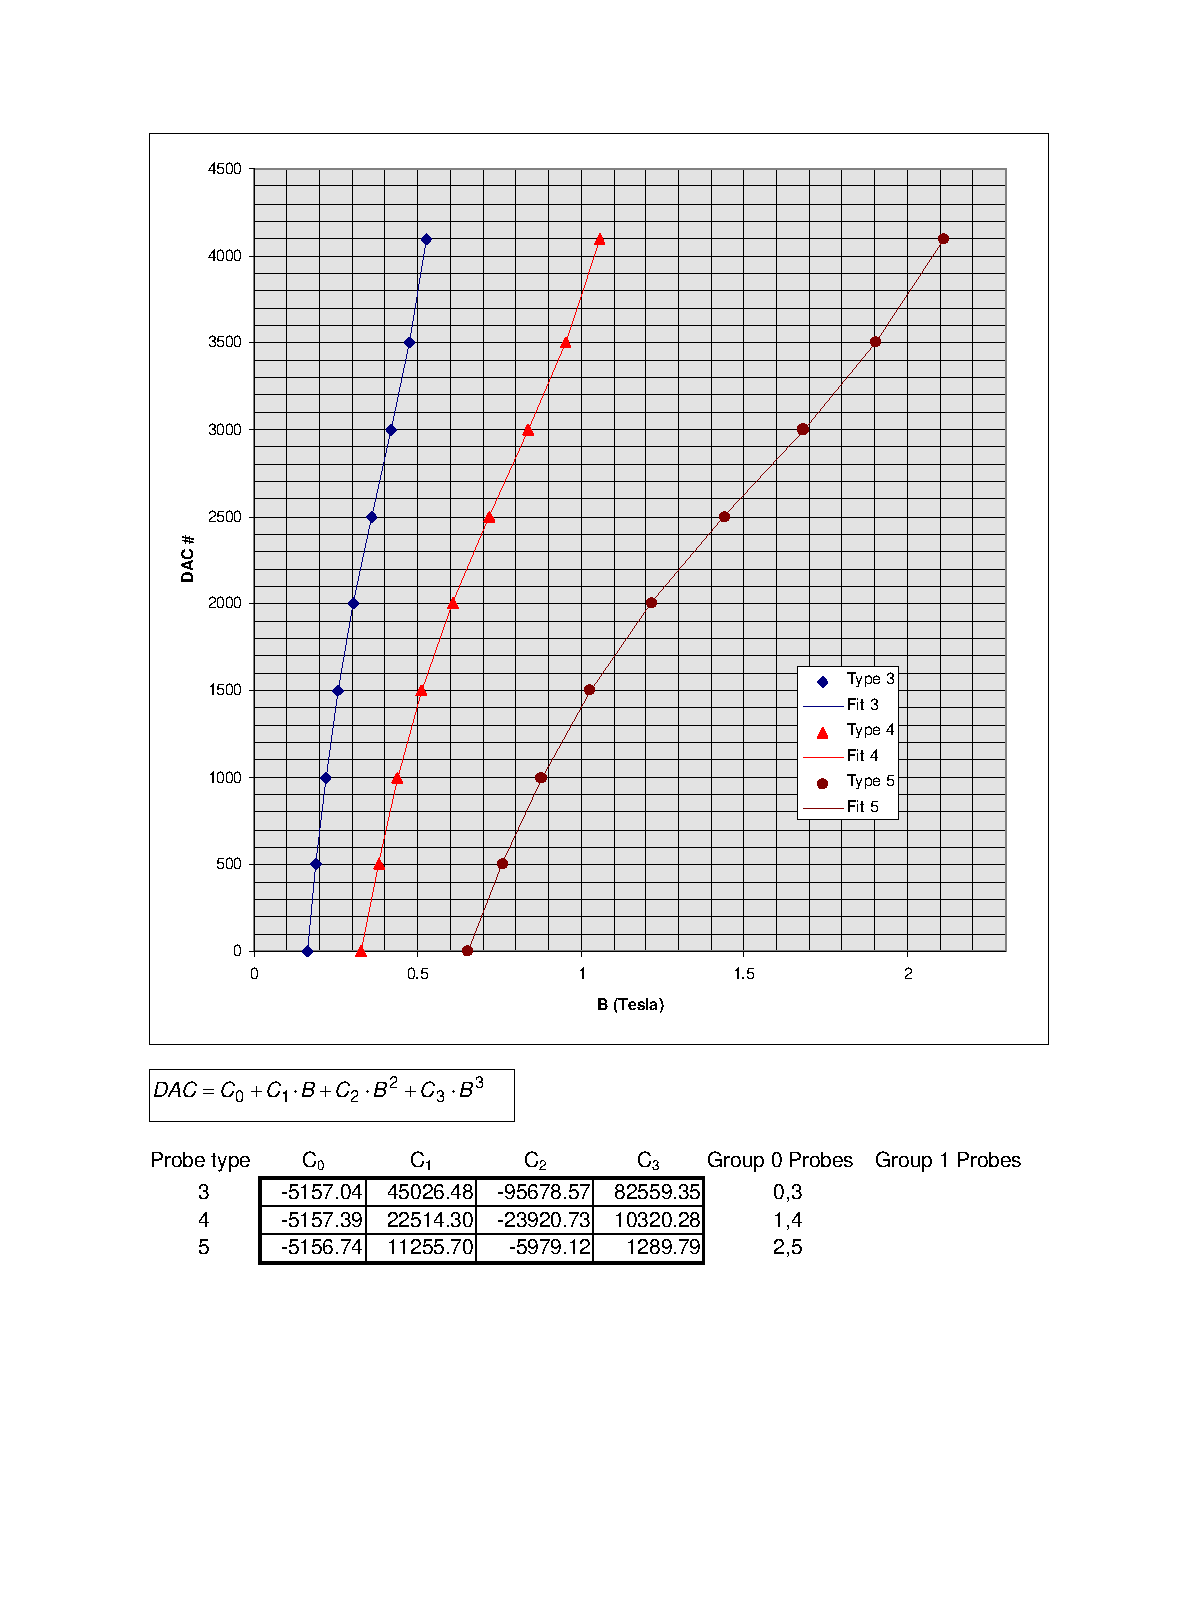
\includegraphics[angle=0,height=20cm,clip]{lerose_fig7}
{\linespread{1.}
\caption[Spectrometers: NMR Probe DAC Calibration]{DAC Calibration for manual operation of NMR probes.}
\label{fig:nmr_dac}}
\end{center}
\end{figure}

The following graphs (see Figures~\ref{fig:nmrcomp4} 
and ~\ref{fig:nmrcomp5}),can be used to determine optimum values for the 
compensating coil control voltage.  It should be noted that the setting 
of the compensating coil current is not very critical in most cases.  In 
general if you're within 10\% of the correct value everything should 
work fine.



\begin{table}
\begin{center}
\begin{tabular}{|cc|} \hline
Probe Type & Field Range (T) \\ \hline 
3 & 0.17 - 0.52 \\
4 & 0.35 - 1.05 \\
5 & 0.70 - 2.10 \\ \hline
\end{tabular}
\caption[Spectrometers: Dipole NMR Probe Field Ranges]{Dipole NMR probe field ranges}
\label{nmr_range}
\end{center}
\end{table}

} %infolev

\infolevtwo{
\subsection{NMR Operating Procedure}

When running in Autopilot mode (see: Simple Spectrometer Field Setting) the 
compensating coil voltage is set automatically and the probe appropriate for 
the field desired is selected. The gaussmeter is placed in SEARCH Mode and the 
dipole power supply software regulator is turned on. In this case the dipole current is 
adjusted to achieve the desired field. The user should just stand 
back and let it work. What follows are instructions for using
the NMR gaussmeter in situations where Autopilot doesn't work or
some special supplemental measurements are required. 

 In principle it is possible to make the field measurements using the 
SEARCH mode in the Teslameter.  In this mode you select a probe and the 
meter explores the whole field range of the probe until it finds and 
"locks" on the resonant signal indicating that it has a field 
measurement.  A ``lock" is indicated on the controls display by an ``L'' to 
the left of the field values.  This has the advantage of simplicity but in practice can 
be time consuming and doesn't always work.  The problem being, in 
situations where there is a lot of noise mixed in with the signal, the 
circuitry has problems distinguishing the signal from the noise and gets 
lost before it ever finds a lock.  The problem is exacerbated when the 
field being measured is at the high end of the probe's range.  In this 
case the search starts at the low end and keeps getting hung up on the 
noise and never gets to the field range of interest.  The solution to 
this problem is to tell the device approximately what field it's looking 
for and use the AUTO mode to find the lock.  In the procedure below that 
is what we will be doing.

In any case, for ``gap probes" (group 0) you must energize and adjust 
the gradient compensating coils for the field ranges to be measured before 
trying to make a measurement.

For studies involving 
10\% changes in the field settings the compensating coil current can be 
set once and left alone.


\noindent\underline{\bf Recommended Procedure:}(turn the {\bf SOFTWARE REGULATOR OFF} for all 
non-autopilot field measurements)\\
For group 0 probes set compensating coils appropriately (see figures).\\
Put the meter in MANUAL mode with SEARCH OFF \\
Select a probe \underline{\bf and} polarity (\underline{\bf Group 0:  
Probes 0, 1, 2 negative; Probes 3, 4, 5 positive}) \\
Type in the appropriate DAC number for the field range being measured (see below) \\
Select AUTO and wait for a lock (indicating a valid field reading) \\
Verify that you have a good lock by checking the oscilloscope for a 
clear resonant signal. \\
If you have problems see the table listing problems and possible 
solutions.

\noindent\underline{\bf Selecting DAC Number}

In selecting the DAC number to use for the field of interest use 
either the graph in Figure~\ref{fig:nmr_dac} or the polynomial at the bottom of the same figure.

\pagebreak
\noindent{\bf Problems and Solutions}\\
\begin{table}[htb]
\begin{tabular}{|p{0.4\textwidth}|p{0.55\textwidth}|}\hline
Symptom & Diagnosis and Cure \\ \hline\hline
Weird numbers on displays, controls for all magnets fouled up 
& Need to reboot.  See instructions below. \\ \hline
NMR Teslameter does not respond to commands and display shows all zeros. 
& Meter's communications are somehow hung up. Push {\bf RESET}. \\ \hline
%Will not lock & Very high noise level makes resonance hard to find. \\
%Still 
Will not lock 
& Very high noise level makes resonance hard to find. Search for the resonance manually by 
  adjusting the DAC in manual mode until you see the resonant signal.  (It helps if you know 
  what field you expect so you'll know where to look). \\ \hline
You find resonance manually but still can't get a lock 
& Check probe polarity. Try decreasing and increasing DAC number by 1. Optimize signal 
  by adjusting compensating coils. \\ \hline
Can't find resonance manually 
& Try a different probe.  Use readings from other probes to tell you where to look for 
 the resonance with the probe that's giving you trouble.  Make sure
 compensating coils are energized properly.  Make sure magnet is on. \\ \hline\hline
\end{tabular}
\caption[NMR: Problems and solutions]{NMR: Problems and solutions}
\label{tab:nmr-problems-solutions}
\end{table}

\begin{table}[ht]
\begin{center}
\begin{tabular}{|p{0.3\textwidth}|p{0.3\textwidth}|p{0.3\textwidth}|}\hline
Problems & Explanation & Action \\ \hline
NMR not locked but current is changing in the right direction 
& Normal operation for large field changes  
& Wait. (see above) \\ \hline
NMR locked but current going in the wrong direction.
& Normal operation. 
& Wait. \\ \hline
NMR locked but field not correct and current not changing 
& Field regulation is disabled or software is confused.
& Check that field regulation is enabled. Enter desired field value or one
  very near the desired value again. \\ \hline
NMR field display freezes. (Usually but not always shows  -\#.0000000)
& NMR Gaussmeter is not communicating with software.
& Push {\bf RESET}. \\ \hline
\end{tabular}
\end{center}
\caption[NMR troubleshhoting]{NMR troubleshooting
}
\label{tab:hrs_nmr_2}
\end{table}

} %infolev

\begin{safetyen}{10}{15}
\subsection{Authorized Personnel}
\end{safetyen}

The individuals shown in Table \ref{tab:nmr:personnel} are responsible for NMR operation problems.

\begin{namestab}{tab:nmr:personnel}{NMR: authorized personnel}{%
      NMR: authorized personnel.}
  \JavierGomez{\em Contact}
  \JohnLeRose{}
\end{namestab}



\newpage
\section[Collimators and Sieve Slits]{Collimators and Sieve Slits
\footnote{
  $CVS~revision~ $Id: slit.tex,v 1.5 2003/12/13 06:23:38 gen Exp $ $ 
}
\footnote{Authors: J.LeRose \email{lerose@jlab.org}}
}

Both spectrometers have front-end devices for calibrating the optical
properties of the spectrometers. These are known as the collimator boxes.
These boxes are positioned between the scattering chamber and the 
first quadrupoles (Q1). Each box is carefully aligned and rigidly attached
to the  entrance flange of the Q1 of the respective spectrometer.  The boxes are
part of the vacuum system of the spectrometer.
In the septum configuration sieve slits and collimators are installed and removed manually.

Inside each box a ladder is mounted which is guided by a linear bearing
and moved up and down by a ball screw. On this ladder 3 positions are 
available to insert collimators. Below this ladder
a special valve is mounted that can isolate the vacuum in the spectrometer
from the target system. This valve should be activated when it is moved
in front of the holes connecting the box with spectrometer and target chamber.
\infolevone{
A schematic view of the collimator box is shown in Fig.~\ref{fig:coll}.

\begin{figure}
\begin{center}
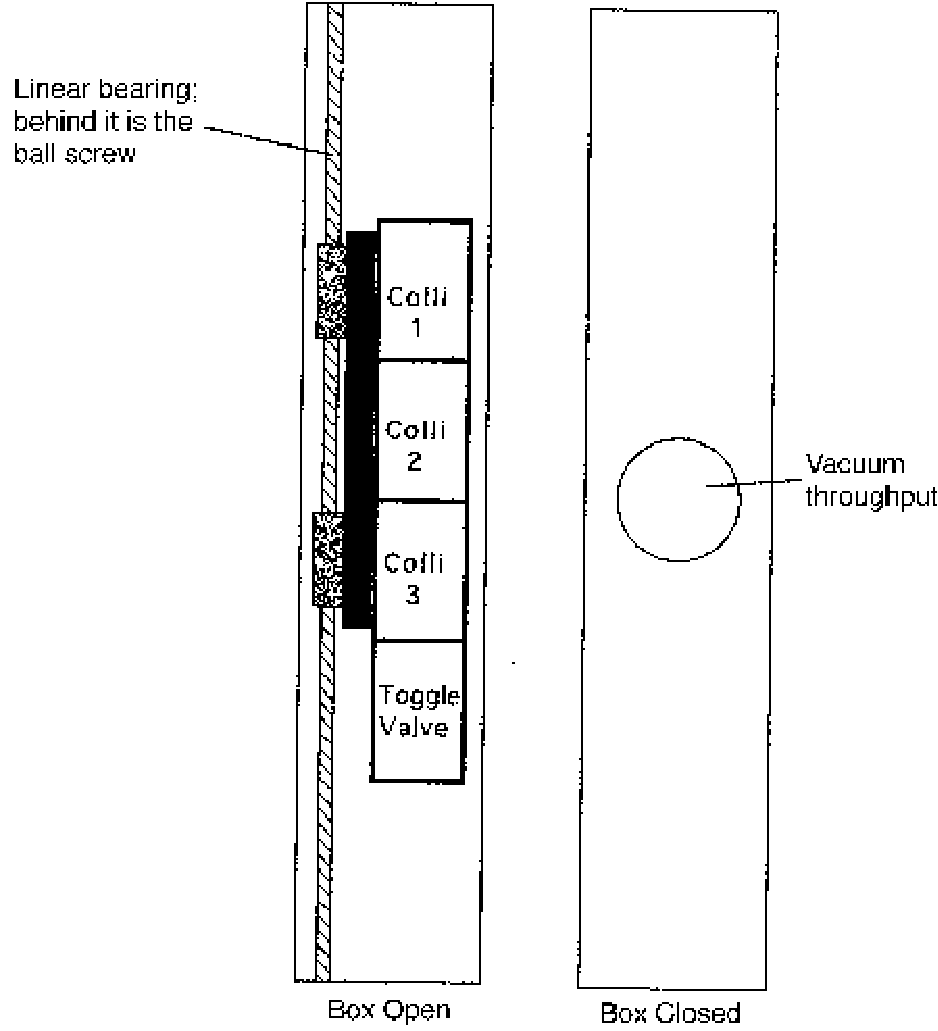
\includegraphics[angle=0,width=13cm,clip]{collimator_clip}
{\linespread{1.}
\caption[Spectrometers: Collimator Box Schematic]{Schematic layout of the collimator box.}
\label{fig:coll}}
\end{center}
\end{figure}
} %infolev

Vacuum requirement is $10^{-6}$ Torr. The material for the box is 
aluminum. It is possible to open one side of the box so that
collimators can be exchanged. The
reproducibility of collimator positions after moving
the ladder and/or after replacing a collimator is
better than 0.1 mm in horizontal and vertical direction.
The dimensions of the box are
roughly height=175 cm , width=35 cm and depth=15 cm.
The tolerance in the dimension
of the 7 msr collimator hole is $\pm0.5$ mm in each direction. 
The tolerance in the position
of each of the sieve-slit holes is $\pm0.1$ mm in each direction.

\infolevone{
\begin{figure}
\begin{center}
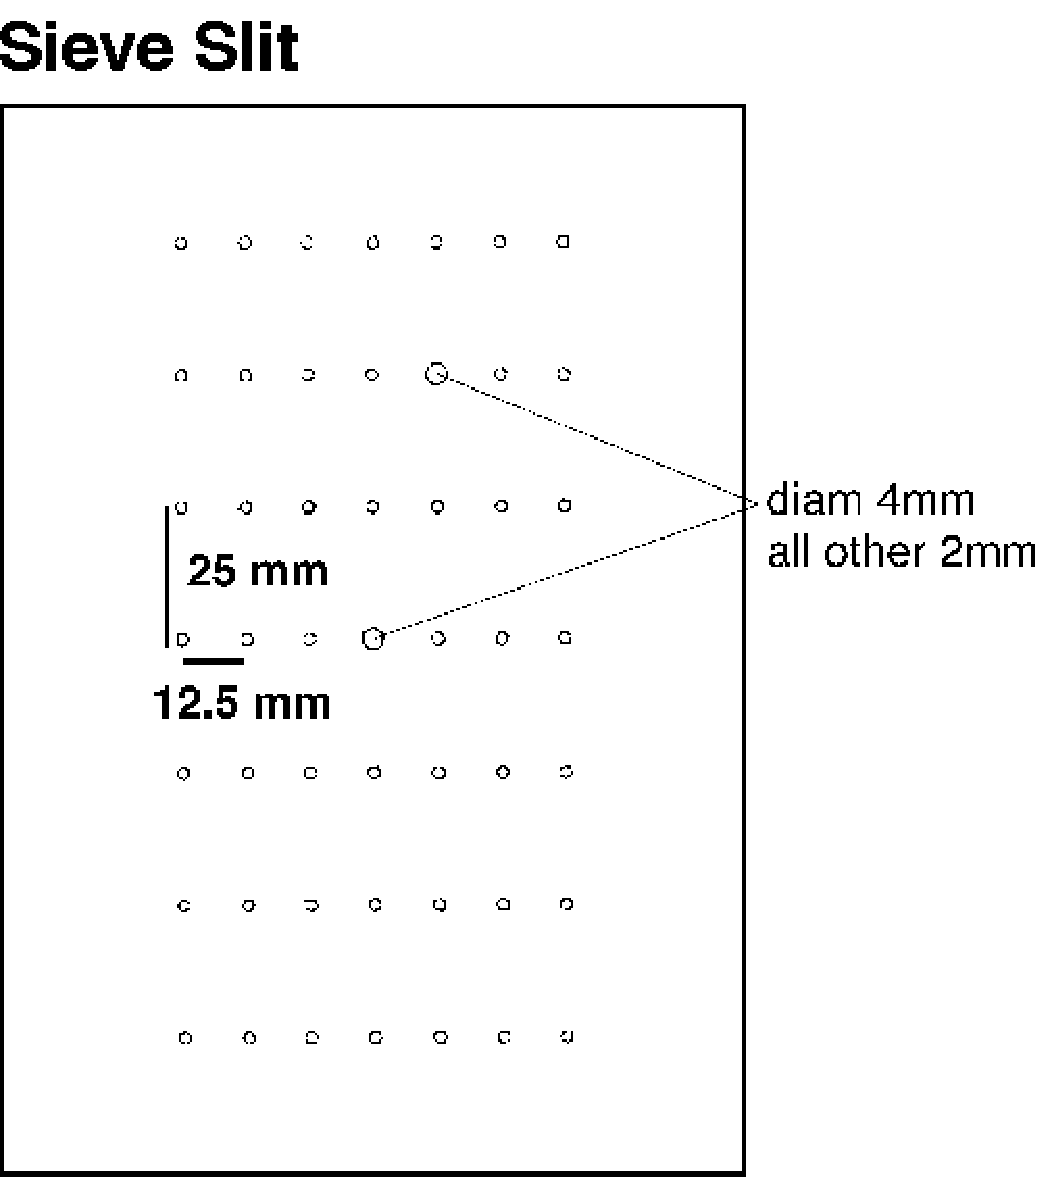
\includegraphics[angle=0,width=13cm,clip]{sieveslit}
{\linespread{1.}
\caption[Spectrometers: Sieve Slit]{Sieve slit collimator for optics calibration.}
\label{fig:sieve}}
\end{center}
\end{figure}
} %infolev
A typical sieve slit collimator 
\infolevone{(shown in Fig.~\ref{fig:sieve})
} %infolev 
consists of a plate of roughly 14 cm x 20 cm containing 49 holes
positioned in a regular 7x7 pattern. This slit is made out of 5
mm thick tungsten.
The holes have a diameter of 2 mm except for the central one and one positioned
off-diagonal which have a diameter of 4 mm. The horizontal distance between the
holes is 12.5 mm while the vertical distance is 25.0 mm.
%
%To get the latest information on the dimensions and locations of the collimators see 
%the Hall A homepage on the web%
%\htmladdnormallinkfoot{}{\url{
%http://hallaweb.jlab.org/
%}}.

To get the latest information on the dimensions and locations of the collimators see 
the Hall A homepage on the web%
\htmladdnormallinkfoot{}{\url{
http://hallaweb.jlab.org/
}}.

\begin{safetyen}{10}{15}
\subsection{Safety Assessment}

The collimator boxes form part of the vacuum system for each spectrometer. All hazards
identified in section spectrometer vacuum section applies to the collimator box as well.

In addition, safe access to the top of
the collimator boxes is needed  during manual operation of the box as outlined below.
Due to the proximity of the collimator boxes to the scattering chamber, and Q1 quadrupoles,
all necessary safety precautions with regards to vacuum windows, electrical power cables, 
cryogenic transfer lines, and high magnetic field should be taken. The same precautions also apply 
to the collimators and sieves in the septum configuration. In that case the sieve and collomators
can be considered part of the beamline. A survey and
appropriate RADCON designated proceedures must be followed when dealing with septum sieves 
and collimators.
\end{safetyen}

\infolevtwo{
\subsection{Operating Procedure}
Slit position is changed remotely from the standard Hall A control screen.
In the case of a spectrometer configuration involving the septum magnets collimators and sieves are
changed manually in the Hall.
} %infolev

\subsection{Authorized  Personnel} 

\begin{itemize} 
\item[~]E. Folts - x7857 (mechanical and vacuum systems).
\item[~]J. Gomez - x7498 (computer controls and electrical systems).
\end{itemize} 

% ===========  CVS info
% $Header: /group/halla/analysis/cvs/tex/osp/src/hrs/slit.tex,v 1.5 2003/12/13 06:23:38 gen Exp $
% $Id: slit.tex,v 1.5 2003/12/13 06:23:38 gen Exp $
% $Author: gen $
% $Date: 2003/12/13 06:23:38 $
% $Name:  $
% $Locker:  $
% $Log: slit.tex,v $
% Revision 1.5  2003/12/13 06:23:38  gen
% Septum added. Name tables. Polishing
%
% Revision 1.4  2003/12/05 06:49:07  gen
% infolevels added, polishing
%
% Revision 1.3  2003/06/06 16:13:37  gen
% Revision printout changed
%
% Revision 1.2  2003/06/05 23:30:00  gen
% Revision ID is printed in TeX
%
% Revision 1.1.1.1  2003/06/05 17:28:31  gen
% Imported from /home/gen/tex/OSP
%
%  Revision parameters to appear on the output

\newpage
\infolevtwo{
\section[Spectrometer Alignment]{Spectrometer Alignment
\footnote{
  $CVS~revision~ $Id: AlignmentOps.tex,v 1.8 2003/12/17 03:59:48 gen Exp $ $ 
}
\footnote{Authors: J.Gomez \email{gomez@jlab.org}}
}

At present, the systems implemented to determine the alignment of each spectrometer
(roll, vertical angle/pointing and horizontal angle/pointing) without the help of the
Accelerator Division Survey group are limited to roll, vertical angle and horizontal angle.
All alignment information is displayed in the ``ALIGNMENT'' mosaic of the ``Hall A
General Tools'' EDM screen%
\infolevtwo{ (see Fig.~\ref{fig:medm-hlamain-tools})}
(``EOS Menu'' $-->$ ``EDM (HLA Main)'' $-->$ ``Hall A Main Menu'' $-->$ ``Tools'').

A bi-axial inclinometer is used to determine the roll and vertical angle (also known as pitch)
of each spectrometer. These inclinometers are attached to the back of the dipoles at the power
supply platform level. The raw inclinometer measurements, in Volts,
are displayed as ``Tilt X'' and ``Tilt Y''. The inclinometer temperature is also given
(`` Tilt T''), in degree Celsius. From these values, the ``ROLL'' and ``PITCH'' values are
calculated.
Agreement between the inclinometer readings and survey measurements
are better than $\pm$ 0.1 mrad over all presently available history.

The horizontal spectrometer angle is determined from floor marks set in
place by the survey group. Floor marks have been placed every 0.5 $^\circ$ covering the useful range of
both spectrometers.
There are two concentric rings of floor marks in the hall. We will concentrate in the
inner ring which covers the angular range of both spectrometers. The outer ring is
similar.
The inner-ring floor marks are located at a distance of $\sim$10 $m$ from the target center.
A ruler attached to each spectrometer dipole runs over the floor marks and it acts as a vernier to interpolate
between marks. The location of a given floor mark on the ruler can be viewed from the Hall A Counting
House through a TV camera (labeled ``Front Camera'') .
The camera is able to move along the length of the ruler so that any
parallax effect can be eliminated. The camera motion is controlled from the ``Tools'' screen
through two push buttons (``FRONT CAMERA'' - ``MOVE +'' and ``MOVE --'').
Two fields in the ``ALIGNMENT'' mosaic
(``Flr Mrk'' and ``Vernier'') allow to input
the values read from the TV monitor. The effective spectrometer angle is then calculated and displayed
as ``Angle''. The application ``HRS Floor Marks'' calculates the floor mark and vernier value
to which the spectrometer should be set
to obtain a given angle. Spectrometer horizontal angle surveys and floor mark determinations
agree to $\pm$ 0.2 mrad.

\newpage
\begin{safetyen}{10}{15}
\subsection{Authorized  Personnel} 
\end{safetyen}
The authorized personnel is shown in table \ref{tab:align:personnel}.
\begin{namestab}{tab:align:personnel}{HRS alignment: authorized personnel}{%
      HRS alignment: authorized personnel.}
  \JessieButler{\em Contact}
\end{namestab}

} %infolev


% ===========  CVS info
% $Header: /group/halla/analysis/cvs/tex/osp/src/hrs/all.tex,v 1.3 2003/06/06 15:44:08 gen Exp $
% $Id: all.tex,v 1.3 2003/06/06 15:44:08 gen Exp $
% $Author: gen $
% $Date: 2003/06/06 15:44:08 $
% $Name:  $
% $Locker:  $
% $Log: all.tex,v $
% Revision 1.3  2003/06/06 15:44:08  gen
% Revision printout changed
%
% Revision 1.2  2003/06/05 23:30:00  gen
% Revision ID is printed in TeX
%
% Revision 1.1.1.1  2003/06/05 17:28:31  gen
% Imported from /home/gen/tex/OSP
%
%  Revision parameters to appear on the output


%\infolevone{
%\chapter{High Resolution Spectrometers (HRS)}
\graphicspath{{hrs/figs/}}
\renewcommand{\dirfig}[0]{hrs/figs}
\renewcommand{\dircur}[0]{hrs}

\infolevone{
\chapter[High Resolution Spectrometers (HRS)]{High Resolution Spectrometers (HRS)
}
\footnote{Authors: J.LeRose \email{lerose@jlab.org}}
}
\label{chap:hrs}

\infolevone{
\section{Overview}
   
The Hall A spectrometers and associated instrumentation are designed to 
perform high resolution and high accuracy experiments.  The goal is to 
achieve a missing mass resolution of $\sim$ 200-500 keV to clearly 
identify the nuclear final state.  An absolute accuracy of $\sim$ 1\% is 
also required by the physics program planned in the Hall, which implies 
$\sim$ 10$^{-4}$ accuracy in the determination of particle momenta and 
$\sim$ 0.1 mr in the knowledge of the scattering angle.

The instruments needed are a high resolution electron spectrometer 
(HRES) and a high resolution hadron spectrometer (HRHS), both with a 
large angular and momentum acceptance.

\begin{figure}[tbp]
\begin{center}
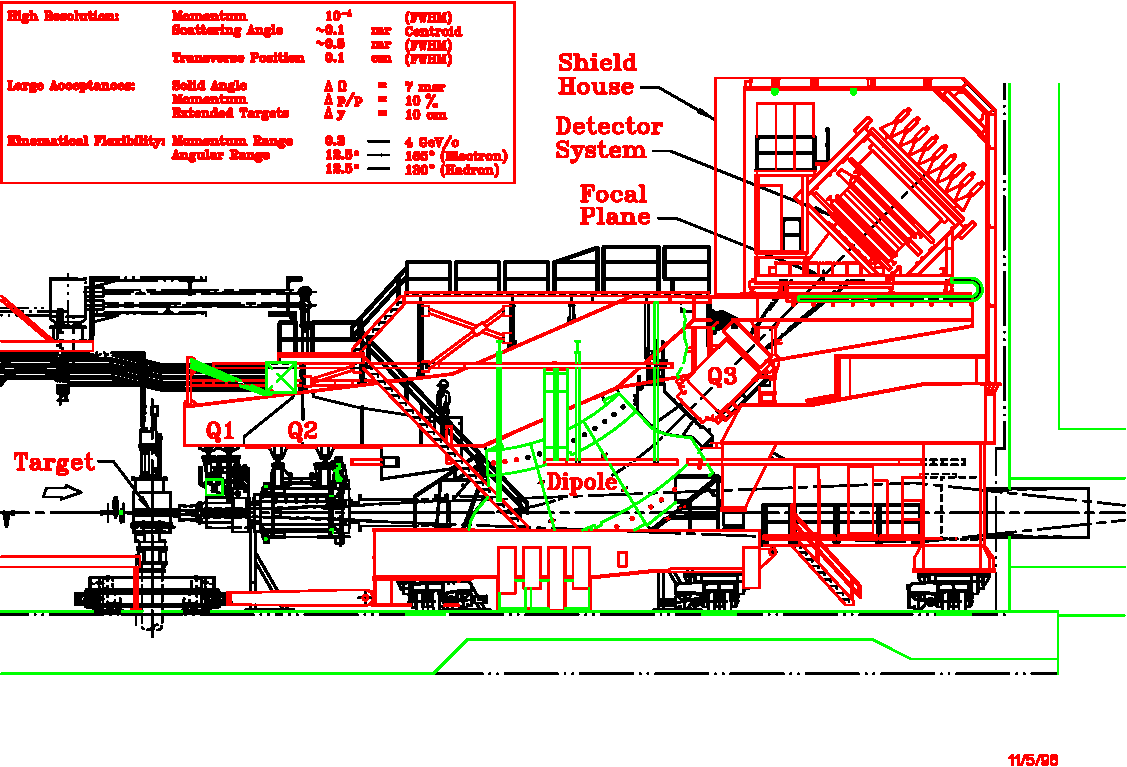
\includegraphics[angle=0,width=0.9\textwidth,clip]{figure0101_r}
\caption[Spectrometers: Elevation View of Hall~A HRS]{A side view of the Hall~A
HRS spectrometer.}  
\label{fig:hrs_ev}
\end{center}
\end{figure}
 
\begin{figure}[tbp]
\begin{center}
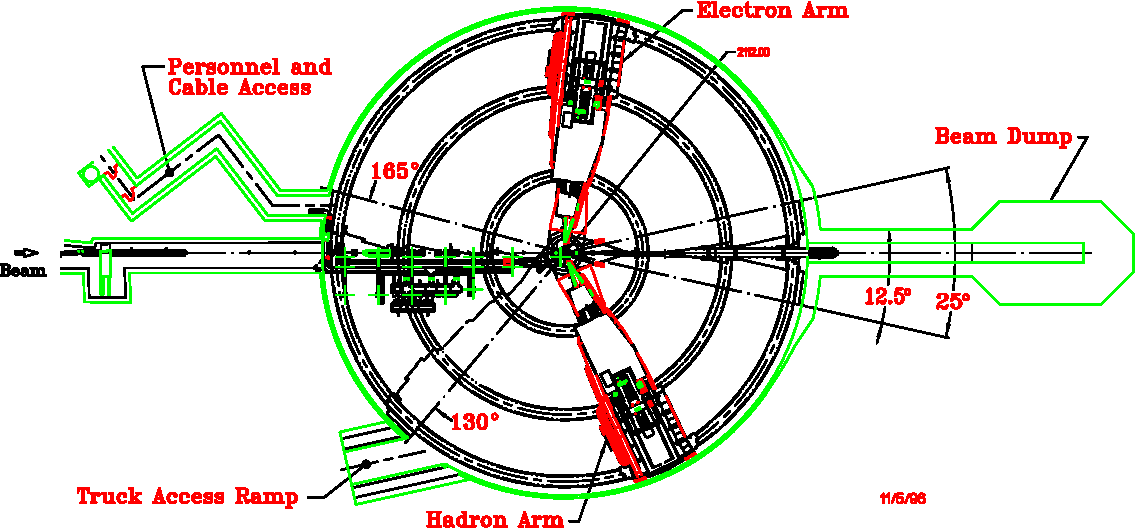
\includegraphics[angle=0,width=0.9\textwidth,clip]{figure0102_r}
\caption[Spectrometers: Plan View of Hall~A]{A bird's eye view of the Hall~A
end-station at TJNAF.}  
\label{fig:hrs_pv}
\end{center}
\end{figure}


A layout of the 4 GeV/c High Resolution Electron Spectrometer is shown 
on Figures~\ref{fig:hrs_pv} and \ref{fig:hrs_ev}.
Its main design characteristics are 
given in the attached table.  The spectrometer has a vertical bending 
plane and 45$^{\circ}$ bending angle.  The QQDQ design includes four 
independent superconducting magnets, three current-dominated 
cos2$\theta $ quadrupoles and one iron-dominated dipole with 
superconducting racetrack coils.  The second and third quadrupoles of 
each spectrometer have sufficiently similar field requirements that they 
are of identical design and construction.  The overall optical length, 
from target to focal plane, is 23.4 m.  Optically, the HRHS 
is essentially identical to HRES. In fact the two spectrometers can be used 
interchangeably to detect either positively or negatively charged particles 
as needed by any particular experiment. They are now commonly refered to 
as ``The Left Arm'' and ``The Right Arms'' rather than ``Hadron'' and ``Electron'' 

The support structure includes all system elements which bear the weight 
of the various spectrometer components and preserve their spatial 
relationship as required for 45$^{\circ}$ vertical bending optics.

The alignment and positioning system includes all the elements which 
measure and adjust the spatial relationship.  The support structure 
consists of the fabricated steel components which support the magnets, 
detector, shield house and associated equipment.  It is composed of the 
box beam, which supports the outer elements in fixed relative position 
atop the dipole; the dipole support bracket, upon which the dipole rests on 
the jacks; the cradle, upon which the dipole rests through the vertical 
positioning system, VPS; and a portion of the shield house load through 
the inboard legs of the gantry; the gantry, which supports the shield 
house and the magnet power supplies; and the bogies, which support the 
cradle-gantry assembly and roll on the floor plates and provide the 
driving power to move the two spectrometer arms.

The detector package (described in detail in Chapter \ref{chap:hrs-det})
is supported on the box beam and is surrounded by 
the shield house.  It must perform two functions, tracking and particle 
identification, PID.  The most important capability of focusing 
spectrometers is measuring precisely the momenta and entrance 
orientations of the tracks.  Momentum resolution of 10$^{-4}$ is 
obtainable, consistent with the resolution of the incident beam.

The actual configuration of the detector package varies from experiment to
experiment. The description given here is only an example of what is possible.
}

\infolevone{
A particle traversing the detector stack 
(Figure~\ref{fig:hrs_electron_det}) encounters two sets of horizontally
mounted, vertical drift wire chambers (x,y) with two planes of 368
wires in each chamber. The track resolution is $\sim$ 100 $\mu$m.  
From the chamber information both 
positions and angles in the dispersive and transverse directions can be 
determined.  The information from these chambers is the principal input 
of the tracking algorithms.

The chambers are followed by a scintillator hodoscope plane designated S1. 
This plastic scintillator array provides the timing reference for 
the drift chambers, and is also used in trigger formation and in combination 
with a second hodoscope pair it can provide time of flight particle 
identification.  These scintillators can also be used to perform crude 
tracking.

The next element encountered by a particle is a gas threshold \Cherenkov{} 
detector.  This is used for particle identification.  This gas threshold \Cherenkov{} detector can be swapped 
against an Aerogel detector, with a similar function.

The second hodoscope plane, S2, is located directly behind the 
gas \Cherenkov{}.  Its function is essentially the same as that of S1.  
In the hadron spectrometer an option exists to have this hodoscope 
pair be preceded by a third chamber, to improve tracking.
 Each of the two spectrometers 
have gas and Aerogel \Cherenkov{} detectors which can be used
 when they are in electron detection mode.

The final elements in the detector stack on HRSE are 
the pre-shower and the total-absorber lead glass shower 
calorimeter.  This is used for energy determination and PID.

\begin{figure}[tbp]
\begin{center}
\includegraphics[angle=0,width=\textwidth,clip]{figure0103_r}
{\linespread{1.}
\caption[Spectrometers: Electron Arm Detectors]{The electron spectrometer detector stack.}
\label{fig:hrs_electron_det}}
\end{center}
\end{figure}

\begin{figure}[tbp]
\begin{center}
\includegraphics[angle=0,width=\textwidth,clip]{figure0104_r}
{\linespread{1.}
\caption[Spectrometers: Hadron Arm Detectors]{The hadron spectrometer detector stack.}
\label{fig:hrs_hadron_det}}
\end{center}
\end{figure}


The hadron detector is shown schematically in 
Figure~\ref{fig:hrs_hadron_det}.  It consists 
of two sets of (x,y) vertical drift wire chambers identical to those of the 
electron arm.  The remaining part of the detection system is used to 
define the level 1 trigger, as well as for particle identification and 
timing.  It consists of two minimally segmented planes of 
scintillation counters equipped with photomultipliers at both ends, and 
it includes \Cherenkov{} counters (gas CO$_2$ and Aerogel).

In addition, a proton polarimeter is installed in the back of the 
detector package to measure the polarization of the proton using a 
segmented carbon analyzer up to 60 cm in thickness to allow measurements 
over a wide range of proton energies.  A pair of front and a pair of 
rear straw tube wire chambers determine the incident and 
scattered angles, respectively.  The 
polarimeter detectors are dimensioned to accept a 20$^{\circ}$ cone of 
scattered protons.

Several support systems are necessary in addition to the basic 
components mentioned above.  They include gas supply systems for the 
wire chambers, high voltage supplies, readout electronics, a second 
level trigger, software for data analysis and testing, and a remotely 
controllable mechanical system.

For each spectrometer, all detectors are mounted on a 
single rigid support frame along with their associated electronics.  The trigger electronics are located on the support frame, next to the detectors.

To reduce the resolution degrading effects of multiple scattering, the 
entire interior of the spectrometer from the collimator box to the detector hut 
is a vacuum vessel.  The ends of this evacuated volume are capped by 
relatively thin vacuum windows.
}

\begin{safetyen}{0}{0}
\section{High Resolution Spectrometers}
\label{sec:hrs-safety}
\end{safetyen}

The principle concern with the spectrometers is that they are large, 
and have associated vacuum, hydraulic, cryogenic and magnet systems all of 
which can be potentially dangerous.

The bogies which move the massive 1200 ton spectrometers must be 
carefully operated.  Inspection of the floor and wheels to ensure there is no 
debris which the wheels could ride over is mandatory.  Similarly 
personnel need to be aware that the spectrometers are moving so that no one 
inadvertently gets trapped.

The vacuum systems associated with the spectrometers are essentially 
pressure vessels (see Chapter \ref{chap:vacuum} for more details).
Care should be exercised so as not to puncture the 
windows.

The magnets themselves are installed inside cryostats.  These vessels 
are exposed to high pressures and are therefore equipped with safety 
relief valves and burst discs.

The hydraulic system originally intended to operate the vertical positioning system (VPS) 
and the horizontal positioning system (HPS) has effectively been dismantled, after problems were encountered during the initial attempted operation of the system.

The cryogenic system operates at elevated pressure at 4K.  One must 
guard against cold burns and take the normal precautions with pressure 
vessels when operating this system.  Only authorized personnel are permitted to install 
and take out U tubes.

The magnets have a great deal of stored energy as they are large 
inductors. Always make sure people are clear of them and that
the dump resistor is attached to the magnet.

There are several major safety concerns with regards to the detectors, 
namely 1) flammable gas located in the VDC, 2) ODH hazard due to 
CO$_2$ in the \Cherenkov{} counter, 3) high voltage due to the photo 
multipliers on the various detectors and 4) a thin vacuum window 
separating the detector array from the vacuum system in the 
spectrometers.

\infolevltone{
\begin{safetyen}{5}{10}
For more information consult the full OSP manual~\cite{HallAosp}.
\end{safetyen}
} %infolev

\begin{safetyen}{10}{15}
\subsection{Authorized Personnel}
\end{safetyen}

In the event that problems arise during 
operation of the magnets, qualified personnel should be notified
(see Table \ref{tab:hrs:personnel}).  
This includes any prolonged or serious problem with the source of magnet 
cryogens (the ESR).  On weekends and after hours there will be a 
designated individual on call for magnet services.  Any member of the 
Hall A technical staff is qualified to deal with unusual magnet 
situations but in the event of serious problems the technician on
call should be contacted.

\begin{namestab}{tab:hrs:personnel}{HRS: authorized personnel}{%
      HRS: authorized personnel. ''W.B'' stands for the white board 
      in the counting house.}
   \TechonCall{\em Contact}
   \EdFolts{}
   \JackSegal{}
   \HeidiFansler{}
   \JessieButler{}
   \AndrewLumanog{}
   \JasonGlorioso{}
   \MahlonLong{}
\end{namestab}

\infolevone{
\section{The Magnets of HRS}

Each HRS is composed of three superconducting quadrupole magnets, Q1, Q2, 
and Q3, and one superconducting dipole magnet.  The large quadrupoles were 
manufactured for JLab by SIEMENS, the small quadrupole by SACLAY, while 
the dipole was built for JLab by WANG NMR.  The quadrupole magnets are 
referred to as Q1, Q2, and Q3, where a particle first traverses Q1, then 
Q2 and the dipole magnet and finally traverses Q3.

The magnet system is followed by a large steel and concrete detector 
hut, in which all detector elements reside.  Most of the 
detector elements have been built by universities involved in the Hall A 
physics program.

The HRS magnet system is the cornerstone of the Hall A activities.  
Many of the experiments approved in Hall A center on physics at high 
resolution and other short-range phenomena, and rely on a spectrometer 
able to momentum analyze charged particles up to very high momenta.  The 
design value for the maximum momentum accessible to the HRS magnet 
system is 4 GeV/c.
}

\subsection{Magnets and Power Supplies}

\infolevone{
The HRS magnet's are all superconducting and hence their coils must be 
maintained at cryogenic temperatures during operations.  The LHe 
required by the magnets is supplied by the End Station Refrigerator, ESR.

All the HRS magnets cryogenic services are supplied through the overhead 
cryogenic lines.  The distribution network begins at the distribution 
box over the pivot.  This box is connected to the rest of the network 
via the flexible transfer lines over the pivot.  The network is adjacent 
to the upstairs catwalk of the HRS.

Cryogenic information about each magnet is available on the control 
screens in the counting house, one for each magnet.  Normally during run 
periods the control screens are sent upstairs to the Hall A counting 
house and information on all the HRS magnets is available on the HRS 
control screen located in the center of the main console.  The control 
of all magnets is described in a following Section.

The power supplies for the magnets are located on the gantry balcony 
adjacent to the magnets.  The supplies are all cooled with low conductivity water (LCW).
}

\begin{safetyen}{10}{15}

Under no 
circumstances should any panel of any magnet power supply be opened by someone 
other than authorized personnel.  There are also 
signs posted listing the dangers of high magnetic fields.
\end{safetyen}

\infolevone{
A control interface for the power supplies is available through the 
HRS control screen in the Hall A counting house.
}

\infolevone{
\subsection{Quadrupole Magnets}

The quadrupoles provide some of the 
focusing properties of the spectrometer and to a large extent 
its acceptance.  Operating limits imposed on the 
quads are as follows: 1850A for Q2 and Q3 and 3250A 
for Q1.

All three quadrupoles for the HRS spectrometer are warm iron 
superconducting magnets.  The soft iron around the superconducting coil 
enhances the field at the coil center and reduces stray fields.  The 
basic parameters for the first quadrupole, Q1, are an effective length of about 
0.9 $m$, useful aperture of 0.3 $m$ and a field gradient of 9.5 
T/m.  To achieve the lowest possible angle setting of the HRS 
spectrometer (with respect to the beam line) the incident electron beam passes through
a notch in the outer yoke of Q1 when the spectrometer is at
its smallest angle of 12.5$^\circ$ . The 
other two quadrupoles, Q2 and Q3, are essentially identical with an 
effective (magnetic) length of about 1.8 meter, a useful aperture of 
0.6 $m$ and a field gradient of 3.5 T/m.
}

\infolevthree{
The maximum operating currents (assuming a 4 GeV/c momentum particle) 
for the quadrupoles are about 3000 A, 1700 A, and 1600 A, for Q1, Q2, and 
Q3, respectively.  This will render pole field values 
of 1.2, 1.0, and 1.0 T, respectively.  The energy stored in the 
quadrupole fields is sufficient to cause an unrecoverable quench if all 
the energy stored is dumped into the magnets.  Therefore a quench 
protection circuit is incorporated.  However, a quench can only happen 
if the cryomagnets have a helium level below the coil 60\% during operation.

The operating current to the Q1 quadrupole coils is provided by Danfysik 
System 8000 power supplies, which can operate up to 3500 A current and 5 
V.  The power supplies will be cooled with a combined maximum 
water flow of 45 liters per minute.

In addition to the main quadrupole windings, all quadrupoles have 
multipole windings.  To further optimize focusing properties of the HRS 
magnet system, it was intended to operate including some of these multipole 
trim coils in order to reduce higher order aberrations.
The operating current for these multipole corrections would be 
small, only (the multipole corrections are typically less than 2\% of 
the main quadrupole field), of order 50 A. Since the sextupoles were inadvertently 
installed rotated 90 $^\circ$ from their correct
orientation, these trim coils are now considered useless 
and there are at present no plans to use them.

\subsection{Cryogenic Procedures}

The cryogenics control is handled by the JLab Cryogenics Group.  The cryo control coordinator 
can be reached at the CHL (x7405) or by calling the MCC.

\subsection{First Time Startup Check List.}  

See attached check lists for all quadrupole and dipole magnets
 (Tables~\ref{tab:dip_check}, \ref{tab:q1_check}, and \ref{tab:q23_check}).
} %infolev

\infolevone{
\subsection{Dipole Magnet}

The dipole, by virtue of its field index, provides both
dispersion and focusing.  The present operations envelope 
states that the supply for the left HRS dipole may not be
operated at a current above 1800 A (4.4 GeV/c). The supply for the right HRS
dipole may not be operated above 1200 A (3.2 GeV/c), due to complications
caused by an internal short. 

The dipole for the HRS spectrometer is a superconducting, cryostable 
magnet.  Its basic parameters are an effective length of about 6.6 $m$, a 
bend radius of 8.4 $m$, and a gap width of 25 $cm$.  It is configured to 
achieve a 45 degree bending angle for 4 GeV/c momentum particles at a 
central field excitation of 1.6 T.  For the HRS dipole to reach 1.6 T 
an operating current of about 1500 A is required.
} %infolev

\infolevthree{
The dipole has been designed to achieve cryostability up to a field of 2 
T, and this property has been extensively tested up to a field of 1.6 T. 
 The cryostable coils are equipped with an energy removal circuit to 
cover the possibility of an unrecoverable quench.  However, this can 
only happen if the helium level drops below the coil during operation.  
The current to the coils will be provided by a Dynapower Corporation power 
supply, which can operate up to 2000 A and 10 V.  This 
power supply is located on the gantry beside the dipole, and will be 
cooled with a maximum water flow of 35 liters per minute.
The total water flow needed to cool the 4 power 
supplies for the HRS magnet system (dipole and quadrupoles) amounts to 
80 liters per minute, with a supply pressure of cooling water for Hall A 
of 100 psi.
} %infolev

\infolevtwo{
\section{Operation of the HRS Magnets}

\subsection{Introduction}

This is an abbreviated operating manual for 
the HRS superconducting magnets specifically designed for Hall A 
experimenters.  It provides instructions for setting currents, invoking 
NMR field regulation and general system monitoring.  Curious readers are 
directed to the references for more in-depth operating instructions and 
other technical manuals. Copies of the following supporting
documents are available in the Hall A Control Room and through the Hall A webpage
(see Table~\ref{tab:hrs-mag-manuals}).

\begin{table}[htp]
\begin{center}
\begin{tabular}{|l|l|}
\hline
References & \\
\hline 
WANG NMR Dipole & User Manual \\
Dynapower & Instruction Manual \\
Appendix & NMR Tesla meter \\
Appendix & NMR Field Regulation \\
Siemens/Fug & Q2/Q3 Magnet Instrumentation and Power Supplies \\
Saclay/Danfysik & Q1 Power Supply Manual \\
TOSP & HRS Dipole \\
TOSP & HRS Quadrupole Q1 \\
TOSP & HRS Quadrupole Q2, Q3 \\
HRS & SC Dipole Magnet Safety Review Vol. 2 \\
HRS & SC Quad Safety Review Vol. 1 \\ \hline
\end{tabular}
\end{center}
\caption[HRS Magnets: extra manuals]{HRS Magnets: extra manuals available in 
     Hall A Control Room.}
\label{tab:hrs-mag-manuals}
\end{table}

\subsection{Simple HRS Setting (Autopilot Mode)}
\label{sec:hrs-mag-set} 

 The magnets are controlled remotely using EPICS~\cite{EPICSwww} and
 EDM~\cite{EDMwww} GUI, provided that everything is working and power 
 supplies are turned on and ready to go.
 The appropriate interface runs
 on the computer \mycomp{hacsbc2} (see Section \ref{sec:contr-ha-menu}).
 On the ``Hall A General Tools'' control screen, in the upper left, there is 
 a rectangular box for each spectrometer (see Figure~\ref{fig:hrs_mag_cntrl}). 
\begin{figure}
\begin{center}
\includegraphics[angle=0,width=0.8\textwidth]{medm_halla_tools_1_cut1}
{\linespread{1.}
\caption[HRS: Magnets control]{A part of ``Hall A General Tools'' screen, 
        used for HRS (left) magnets control.}
\label{fig:hrs_mag_cntrl}}
\end{center}
\end{figure}

This box displays a brief summary of the status of the spectrometer
magnets and their cryogenic systems. The blue fields (with white
numbers) give readbacks of the magnetic fields and currents in each
magnet. The black fields also give readbacks, however in this case if
the text appears green those parameters are OK while if they are red
then that parameter is out of tolerance and may indicate a fault
condition. For example if the helium level goes below a certain point
the magnet will be automatically turned off.  In some cases it may be
desirable to monitor certain critical quantities on a strip chart
(e.g. magnet settings). A strip chart tool is available for this
purpose from the bottom of the ''EOS Menu'' button in the ''MyMenu'' window.

{\bf To set the spectrometers} for a given value of central momentum
(P0) type the desired P0 value into the light blue P0 SET box and hit
return. The magnets will be automatically 
set to the correct
values. All green numbers in the P0 column indicates that the desired
field or current settings have been reached. 

{\bf Caution:} Regarding the
dipoles, in general it's a bad idea to assume that at the first
instant that the P0 display turns green that the desired field has
been reached and you can start taking data. Stable field is in general
not achieved for from 15 to 30 minutes after reaching the nominal
desired field. This settling time depends on the magnet (the right dipole is
slower than the left dipole) and the magnitude of the field change (small
changes settle faster than big changes). Experimenters are advised to
observe both the field reading and current reading on the magnet in
question and verify that things are stable to their satisfaction
before proceeding.
 
\subsection{Powering Up Dipole Magnets:}

Use these instructions to recover from loss of a magnet due to a fault
(e.g. He level or lead flow fault). The order of actions matters. \\
(Contact Tech-On-Call if anything behaves funny or things don't
respond as expected. Sometimes after a trip an access to the Hall is
required to reset things).

\begin{list}{\arabic{enumi}.~}{\usecounter{enumi}\setlength{\itemsep}{-0.15cm}}
   \item Wait for Iout=0 (you can't and don't want to do anything while the magnet is in emergency fast dump mode.)
   \item While waiting, make a log entry re the fault. Give details such as time, coincident activities, and nature of the fault.
   \item Make sure the fault is cleared. (e.g. He level and flow rates returned to normal values and stable)
   \item In the HRS Right (Left) Dipole Systems' control panel:
   \begin{list}{}{\setlength{\itemsep}{-0.15cm}}
      \item[(a)] Press RESET (verify that all faults are cleared in the middle column)
      \item[(b)] Press ON (Display will indicate Power Supply ON and Magnet ENGAGED)
   \end{list}
\end{list}


Power supply and magnet are ready to go. From here you can return 
to "Autopilot Mode" (see Section \ref{sec:hrs-mag-set}).

\subsection{Starting Q1 Power Supply:}

 Do this when a fault causes the power supply to shut off.
 Wait for fault to clear (watch He levels). 
\begin{list}{\arabic{enumi}.~}{\usecounter{enumi}\setlength{\itemsep}{-0.15cm}}
   \item Push POWER OFF/RESET (check all faults cleared)
   \item Select desired polarity
   \item Push POWER ON
   \item Type in Setpoint (Amps) (light blue field) or re-enter P0 in Autopilot Mode.
\end{list}

\subsection{Starting Q2/3 Power Supply:}

 Do this when a fault causes the power supply to shut off.
 Wait for cause of fault to clear (watch He levels). 
 \begin{list}{\arabic{enumi}.~}{\usecounter{enumi}\setlength{\itemsep}{-0.15cm}}
   \item Push RESET 
   \item Select desired polarity
   \item Push ON
   \item Type in Current Set (light blue field) or re-enter P0 in Autopilot Mode.
\end{list}

} %infolev

\subsection{Rotation}
%
% Thanks to John LeRose for Rotation text. 07NOV2013
%
Moving an HRS
Since each HRS weighs in excess of 1,000 tons it is very important that all safety
precautions are carefully adhered to. The good news is they move very slowly (a few degrees/min
maximum), BUT 1,000 tons moving even very slowly is hard to stop. 

Hazards include:
\begin{itemize}
\item{Knocking items over.}
\item{The wheels crushing things (including fingers and toes) on the floor in the path of the 
spectrometer}
\item{Damaging the beamline or other equipment on the floor if one goes to too small 
or too large an angle, or if it just gets pushed around inadvertantly.}
\item{Tearing out of cables etc. physically attached to the superstructure}
\end{itemize}

Hazard mitigations:
\begin{itemize}
\item{Guards on either side of the wheels prevent items from getting under them.}
\item{Large pins in the floor to stop the spectrometer rotated beyond the needed angular range.}
\item{Blinking lights on the spectrometers indicating they are in motion or that motion
is possible (controls engaged etc.)}
\item{During a running experiment the run coordinator and work coordinator should know in advance 
of any moves.  Moves at any other time must be cleared with the Hall work coordinator 
before implementation.}
\item{Careful inspection of the intended path to make sure it is clear. This is part of
the pre-run checklist performed by the technical staff prior to closing the Hall and
a remote camera allows shift worker to inspect the area.}
%
%\item{Any motion that takes a spectrometer inside 14 degrees or outside x degrees
%(x being specified in the pre-run checklist and noted on the whiteboard during a run) 
%must be supervised by a trained Hall A technician.}
\end{itemize}

\infolevone{
Remote Procedure for a shift worker:
\begin{itemize}
\item{Make sure the move is part of the approved runplan (if in doubt, check with the 
run coordinator).}
\item{Check that the pre-run checklist has been completed and note and comply with any 
possible limitations to spectrometer motion (if there is a conflict inform the Run
Coordinator and do not initiate any move until the conflict is cleared).}
\item{Visually inspect the Hall using the closed circuit TV cameras to verify that there
are no obstructions.}
\item{If people are in the Hall wait until they leave (during a Controlled Access MCC keeps
track of people in the Hall). (Maybe we could soften this to "Inform EVERYONE in the Hall of
the move".)}
\item{Activate the spectrometer motion controls (see the Wiki and below) and 
move to the desired angle.}
\item{Deactivate the controls (brakes on, power off, etc.)}
\item{Update the spectrometer position information on the Hall A Controls screen}
\item{Make a halog entry indicating you've moved the spectrometer including from what angle 
to what new angle.}
\end{itemize}

Procedure for a non-run associated move in the Hall:
\begin{itemize}
\item{Inform the work coordinator of the planned move}
\item{Perform a careful visual inspection to verify that the path is clear}
\item{Check to make sure there are no temporary connections to the spectrometer (wires etc.)
that could be damaged during the move.}
\item{Inform everyone in the Hall of the move and check with them re 3.}
\item{Activate the spectrometer motion controls (see the Wiki and below) verify 
that the warning lights are on and move to the desired angle.}
\item{Deactivate the controls (brakes on, power off, etc.).}
\end{itemize}

The full proceedure for moving the spectrometer follows and can also be found on the Hall A wiki.

On hacsbc2, click the red "tool box" icon on the linux taskbar, as above. Choose 
bogies\_SetSpec so that you can determine the angle and vernier setting for the spectrometer.
Enter the spectrometer (L or R), and the angle, and you will get two options for the floor 
mark and the vernier. Generally choose the vernier closer to zero. Center the cameras on the 
desire vernier using the Move+/Move- buttons on the Hall A General Tools screen. The TV monitors 
for these cameras are on the middle shelf, in rack CH01A05.

Choose bogies\_Left (or bogies\_Right) in the tool box to bring up the bogies control screen. 
Click PSM enable and wait a few seconds for PSM OK to read YES. 
Click DM enable and wait a few seconds for DM OK to read YES.
Make sure the velocity is set to 0 and the direction is CW or CCW as desired. Click on Brake Release 
and wait for Brakes OK to read YES.

Click on ClampRelease, set the velocity to 700. Once you see the spectrometer start to move in the 
floor angle camera - you cannot see the spectrometer move in the Hall overview camera, as it only 
moves a few degrees per minute at maximum speed. For the left arm, to move to a larger angle, the 
direction should be CCW, while for the right arm CW moves the spectrometer to larger angle. The 
direction of the spectrometer is reversed by using a negative rpm. Watch the spectrometer motion 
on the cameras. When you are getting close to the desired angle, slow down to about 300 rpm. 
To stop, click on the Clamp Release button and the Brake button. Disable DM and PSM, and disconnect 
to close the GUI. Read off the floor angle mark and vernier, and input the values into the appropriate 
fields in the Alignment section of the Hall A General Tools GUI. 
}









\newpage
\section[Field Monitoring]{Field Monitoring
\footnote{
  $CVS~revision~ $Id: nmr-1999.tex,v 1.4 2003/12/17 03:59:48 gen Exp $ $ 
}
\footnote{Authors: J.LeRose \email{lerose@jlab.org}}
}

The field-monitoring controls are available using the main 
HRS screen%
\infolevtwo{ (see Figure~\ref{fig:hrs_mag_cntrl})%
}. % infolev
The dipoles' field is measured using NMR Teslameters and
field probes.

\infolevone{ 
 
\subsection{ Dipole Field Monitoring Electron Arm}

\noindent {\bf Basic Setup}

Each spectrometer dipole magnet is equipped with a Metrolab PT 4025 
NMR Teslameter, several field probes, and multiplexers (to allow switching 
between the probes).  Details of the operation and theory of operation 
for the Teslameter can be found in its user manual, 
a copy of which is available in the the counting house.
The basic layout is shown in Figure~\ref{fig:nmrbasic}


\begin{figure}
\begin{center}
\includegraphics[angle=0,width=15cm,clip]{lerose_fig1}
{\linespread{1.}
\caption[Spectrometers: NMR System Layout]{Basic layout of NMR system}
\label{fig:nmrbasic}}
\end{center}
\end{figure}


 The "Gap Probes" (Group 0 in the controls) are located in two groups 
of three; one group on the low field side of the gap and the other on the high 
field side of the gap.  The groups of three are made up of one each of 
the manufacturer's type 3, 4 \& 5 probes, designed to cover different 
field ranges (see Table \ref{nmr_range}).  The six ``Purcell Gap Probes'' (Group 1 in 
the controls) are located in the Purcell gap of the magnet 
and consists of two each of the above types. {\em Note: Since
the fall of 1998 the multiplexer-multiplexer in both arms,
MUX 2032, has been removed and hence the ``Purcell Gap Probes'' are currently
unavailable. There are no plans to re-install this multiplexer.}

 The "Gap Probes" are equipped with coils which provide a field 
gradient that cancels out the field gradient of the magnet in the vicinity of 
the probe.  These gradient compensating coils are part of a simple circuit 
that is completely independent of the Teslameter.  The basic circuit for 
the compensating coils is shown in Figure~\ref{fig:nmrcir}


\begin{figure}
\begin{center}
\includegraphics[angle=0,width=10cm,clip]{lerose_fig2}
{\linespread{1.}
\caption[Spectrometers: NMR Gradient Compensation]{Gradient Compensating Circuit.}
\label{fig:nmrcir}}
\end{center}
\end{figure}


%\snfig{figs/lerose_figcce.eps}{Control Voltage calibration for
%Electron Dipole }{nmrcomp4}{5in}

\begin{figure}
\begin{center}
\includegraphics[angle=0,height=20cm,clip]{lerose_figcce}
{\linespread{1.}
\caption[Spectrometers: Control Voltage Calibration for Left Dipole]{Control Voltage calibration for the Left Dipole.}
\label{fig:nmrcomp4}}
\end{center}
\end{figure}

%\snfig{figs/lerose_figcch.eps}{Control Voltage calibration for
%Hadron Dipole }{nmrcomp5}{5in}
\begin{figure}
\begin{center}
\includegraphics[angle=0,height=20cm,clip]{lerose_figcch}
{\linespread{1.}
\caption[Spectrometers: Control Voltage Calibration for Right Dipole] {Control Voltage calibration for the Right Dipole.}
\label{fig:nmrcomp5}}
\end{center}
\end{figure}

%\snfig{./figs/lerose_fig7.eps}{DAC Calibration for manual operation of NMR probes}{nmr_dac}{9in}
\begin{figure}
\begin{center}
\includegraphics[angle=0,height=20cm,clip]{lerose_fig7}
{\linespread{1.}
\caption[Spectrometers: NMR Probe DAC Calibration]{DAC Calibration for manual operation of NMR probes.}
\label{fig:nmr_dac}}
\end{center}
\end{figure}

The following graphs (see Figures~\ref{fig:nmrcomp4} 
and ~\ref{fig:nmrcomp5}),can be used to determine optimum values for the 
compensating coil control voltage.  It should be noted that the setting 
of the compensating coil current is not very critical in most cases.  In 
general if you're within 10\% of the correct value everything should 
work fine.



\begin{table}
\begin{center}
\begin{tabular}{|cc|} \hline
Probe Type & Field Range (T) \\ \hline 
3 & 0.17 - 0.52 \\
4 & 0.35 - 1.05 \\
5 & 0.70 - 2.10 \\ \hline
\end{tabular}
\caption[Spectrometers: Dipole NMR Probe Field Ranges]{Dipole NMR probe field ranges}
\label{nmr_range}
\end{center}
\end{table}

} %infolev

\infolevtwo{
\subsection{NMR Operating Procedure}

When running in Autopilot mode (see: Simple Spectrometer Field Setting) the 
compensating coil voltage is set automatically and the probe appropriate for 
the field desired is selected. The gaussmeter is placed in SEARCH Mode and the 
dipole power supply software regulator is turned on. In this case the dipole current is 
adjusted to achieve the desired field. The user should just stand 
back and let it work. What follows are instructions for using
the NMR gaussmeter in situations where Autopilot doesn't work or
some special supplemental measurements are required. 

 In principle it is possible to make the field measurements using the 
SEARCH mode in the Teslameter.  In this mode you select a probe and the 
meter explores the whole field range of the probe until it finds and 
"locks" on the resonant signal indicating that it has a field 
measurement.  A ``lock" is indicated on the controls display by an ``L'' to 
the left of the field values.  This has the advantage of simplicity but in practice can 
be time consuming and doesn't always work.  The problem being, in 
situations where there is a lot of noise mixed in with the signal, the 
circuitry has problems distinguishing the signal from the noise and gets 
lost before it ever finds a lock.  The problem is exacerbated when the 
field being measured is at the high end of the probe's range.  In this 
case the search starts at the low end and keeps getting hung up on the 
noise and never gets to the field range of interest.  The solution to 
this problem is to tell the device approximately what field it's looking 
for and use the AUTO mode to find the lock.  In the procedure below that 
is what we will be doing.

In any case, for ``gap probes" (group 0) you must energize and adjust 
the gradient compensating coils for the field ranges to be measured before 
trying to make a measurement.

For studies involving 
10\% changes in the field settings the compensating coil current can be 
set once and left alone.


\noindent\underline{\bf Recommended Procedure:}(turn the {\bf SOFTWARE REGULATOR OFF} for all 
non-autopilot field measurements)\\
For group 0 probes set compensating coils appropriately (see figures).\\
Put the meter in MANUAL mode with SEARCH OFF \\
Select a probe \underline{\bf and} polarity (\underline{\bf Group 0:  
Probes 0, 1, 2 negative; Probes 3, 4, 5 positive}) \\
Type in the appropriate DAC number for the field range being measured (see below) \\
Select AUTO and wait for a lock (indicating a valid field reading) \\
Verify that you have a good lock by checking the oscilloscope for a 
clear resonant signal. \\
If you have problems see the table listing problems and possible 
solutions.

\noindent\underline{\bf Selecting DAC Number}

In selecting the DAC number to use for the field of interest use 
either the graph in Figure~\ref{fig:nmr_dac} or the polynomial at the bottom of the same figure.

\pagebreak
\noindent{\bf Problems and Solutions}\\
\begin{table}[htb]
\begin{tabular}{|p{0.4\textwidth}|p{0.55\textwidth}|}\hline
Symptom & Diagnosis and Cure \\ \hline\hline
Weird numbers on displays, controls for all magnets fouled up 
& Need to reboot.  See instructions below. \\ \hline
NMR Teslameter does not respond to commands and display shows all zeros. 
& Meter's communications are somehow hung up. Push {\bf RESET}. \\ \hline
%Will not lock & Very high noise level makes resonance hard to find. \\
%Still 
Will not lock 
& Very high noise level makes resonance hard to find. Search for the resonance manually by 
  adjusting the DAC in manual mode until you see the resonant signal.  (It helps if you know 
  what field you expect so you'll know where to look). \\ \hline
You find resonance manually but still can't get a lock 
& Check probe polarity. Try decreasing and increasing DAC number by 1. Optimize signal 
  by adjusting compensating coils. \\ \hline
Can't find resonance manually 
& Try a different probe.  Use readings from other probes to tell you where to look for 
 the resonance with the probe that's giving you trouble.  Make sure
 compensating coils are energized properly.  Make sure magnet is on. \\ \hline\hline
\end{tabular}
\caption[NMR: Problems and solutions]{NMR: Problems and solutions}
\label{tab:nmr-problems-solutions}
\end{table}

\begin{table}[ht]
\begin{center}
\begin{tabular}{|p{0.3\textwidth}|p{0.3\textwidth}|p{0.3\textwidth}|}\hline
Problems & Explanation & Action \\ \hline
NMR not locked but current is changing in the right direction 
& Normal operation for large field changes  
& Wait. (see above) \\ \hline
NMR locked but current going in the wrong direction.
& Normal operation. 
& Wait. \\ \hline
NMR locked but field not correct and current not changing 
& Field regulation is disabled or software is confused.
& Check that field regulation is enabled. Enter desired field value or one
  very near the desired value again. \\ \hline
NMR field display freezes. (Usually but not always shows  -\#.0000000)
& NMR Gaussmeter is not communicating with software.
& Push {\bf RESET}. \\ \hline
\end{tabular}
\end{center}
\caption[NMR troubleshhoting]{NMR troubleshooting
}
\label{tab:hrs_nmr_2}
\end{table}

} %infolev

\begin{safetyen}{10}{15}
\subsection{Authorized Personnel}
\end{safetyen}

The individuals shown in Table \ref{tab:nmr:personnel} are responsible for NMR operation problems.

\begin{namestab}{tab:nmr:personnel}{NMR: authorized personnel}{%
      NMR: authorized personnel.}
  \JavierGomez{\em Contact}
  \JohnLeRose{}
\end{namestab}



\newpage
\section[Collimators and Sieve Slits]{Collimators and Sieve Slits
\footnote{
  $CVS~revision~ $Id: slit.tex,v 1.5 2003/12/13 06:23:38 gen Exp $ $ 
}
\footnote{Authors: J.LeRose \email{lerose@jlab.org}}
}

Both spectrometers have front-end devices for calibrating the optical
properties of the spectrometers. These are known as the collimator boxes.
These boxes are positioned between the scattering chamber and the 
first quadrupoles (Q1). Each box is carefully aligned and rigidly attached
to the  entrance flange of the Q1 of the respective spectrometer.  The boxes are
part of the vacuum system of the spectrometer.
In the septum configuration sieve slits and collimators are installed and removed manually.

Inside each box a ladder is mounted which is guided by a linear bearing
and moved up and down by a ball screw. On this ladder 3 positions are 
available to insert collimators. Below this ladder
a special valve is mounted that can isolate the vacuum in the spectrometer
from the target system. This valve should be activated when it is moved
in front of the holes connecting the box with spectrometer and target chamber.
\infolevone{
A schematic view of the collimator box is shown in Fig.~\ref{fig:coll}.

\begin{figure}
\begin{center}
\includegraphics[angle=0,width=13cm,clip]{collimator_clip}
{\linespread{1.}
\caption[Spectrometers: Collimator Box Schematic]{Schematic layout of the collimator box.}
\label{fig:coll}}
\end{center}
\end{figure}
} %infolev

Vacuum requirement is $10^{-6}$ Torr. The material for the box is 
aluminum. It is possible to open one side of the box so that
collimators can be exchanged. The
reproducibility of collimator positions after moving
the ladder and/or after replacing a collimator is
better than 0.1 mm in horizontal and vertical direction.
The dimensions of the box are
roughly height=175 cm , width=35 cm and depth=15 cm.
The tolerance in the dimension
of the 7 msr collimator hole is $\pm0.5$ mm in each direction. 
The tolerance in the position
of each of the sieve-slit holes is $\pm0.1$ mm in each direction.

\infolevone{
\begin{figure}
\begin{center}
\includegraphics[angle=0,width=13cm,clip]{sieveslit}
{\linespread{1.}
\caption[Spectrometers: Sieve Slit]{Sieve slit collimator for optics calibration.}
\label{fig:sieve}}
\end{center}
\end{figure}
} %infolev
A typical sieve slit collimator 
\infolevone{(shown in Fig.~\ref{fig:sieve})
} %infolev 
consists of a plate of roughly 14 cm x 20 cm containing 49 holes
positioned in a regular 7x7 pattern. This slit is made out of 5
mm thick tungsten.
The holes have a diameter of 2 mm except for the central one and one positioned
off-diagonal which have a diameter of 4 mm. The horizontal distance between the
holes is 12.5 mm while the vertical distance is 25.0 mm.
%
%To get the latest information on the dimensions and locations of the collimators see 
%the Hall A homepage on the web%
%\htmladdnormallinkfoot{}{\url{
%http://hallaweb.jlab.org/
%}}.

To get the latest information on the dimensions and locations of the collimators see 
the Hall A homepage on the web%
\htmladdnormallinkfoot{}{\url{
http://hallaweb.jlab.org/
}}.

\begin{safetyen}{10}{15}
\subsection{Safety Assessment}

The collimator boxes form part of the vacuum system for each spectrometer. All hazards
identified in section spectrometer vacuum section applies to the collimator box as well.

In addition, safe access to the top of
the collimator boxes is needed  during manual operation of the box as outlined below.
Due to the proximity of the collimator boxes to the scattering chamber, and Q1 quadrupoles,
all necessary safety precautions with regards to vacuum windows, electrical power cables, 
cryogenic transfer lines, and high magnetic field should be taken. The same precautions also apply 
to the collimators and sieves in the septum configuration. In that case the sieve and collomators
can be considered part of the beamline. A survey and
appropriate RADCON designated proceedures must be followed when dealing with septum sieves 
and collimators.
\end{safetyen}

\infolevtwo{
\subsection{Operating Procedure}
Slit position is changed remotely from the standard Hall A control screen.
In the case of a spectrometer configuration involving the septum magnets collimators and sieves are
changed manually in the Hall.
} %infolev

\subsection{Authorized  Personnel} 

\begin{itemize} 
\item[~]E. Folts - x7857 (mechanical and vacuum systems).
\item[~]J. Gomez - x7498 (computer controls and electrical systems).
\end{itemize} 

% ===========  CVS info
% $Header: /group/halla/analysis/cvs/tex/osp/src/hrs/slit.tex,v 1.5 2003/12/13 06:23:38 gen Exp $
% $Id: slit.tex,v 1.5 2003/12/13 06:23:38 gen Exp $
% $Author: gen $
% $Date: 2003/12/13 06:23:38 $
% $Name:  $
% $Locker:  $
% $Log: slit.tex,v $
% Revision 1.5  2003/12/13 06:23:38  gen
% Septum added. Name tables. Polishing
%
% Revision 1.4  2003/12/05 06:49:07  gen
% infolevels added, polishing
%
% Revision 1.3  2003/06/06 16:13:37  gen
% Revision printout changed
%
% Revision 1.2  2003/06/05 23:30:00  gen
% Revision ID is printed in TeX
%
% Revision 1.1.1.1  2003/06/05 17:28:31  gen
% Imported from /home/gen/tex/OSP
%
%  Revision parameters to appear on the output

\newpage
\infolevtwo{
\section[Spectrometer Alignment]{Spectrometer Alignment
\footnote{
  $CVS~revision~ $Id: AlignmentOps.tex,v 1.8 2003/12/17 03:59:48 gen Exp $ $ 
}
\footnote{Authors: J.Gomez \email{gomez@jlab.org}}
}

At present, the systems implemented to determine the alignment of each spectrometer
(roll, vertical angle/pointing and horizontal angle/pointing) without the help of the
Accelerator Division Survey group are limited to roll, vertical angle and horizontal angle.
All alignment information is displayed in the ``ALIGNMENT'' mosaic of the ``Hall A
General Tools'' EDM screen%
\infolevtwo{ (see Fig.~\ref{fig:medm-hlamain-tools})}
(``EOS Menu'' $-->$ ``EDM (HLA Main)'' $-->$ ``Hall A Main Menu'' $-->$ ``Tools'').

A bi-axial inclinometer is used to determine the roll and vertical angle (also known as pitch)
of each spectrometer. These inclinometers are attached to the back of the dipoles at the power
supply platform level. The raw inclinometer measurements, in Volts,
are displayed as ``Tilt X'' and ``Tilt Y''. The inclinometer temperature is also given
(`` Tilt T''), in degree Celsius. From these values, the ``ROLL'' and ``PITCH'' values are
calculated.
Agreement between the inclinometer readings and survey measurements
are better than $\pm$ 0.1 mrad over all presently available history.

The horizontal spectrometer angle is determined from floor marks set in
place by the survey group. Floor marks have been placed every 0.5 $^\circ$ covering the useful range of
both spectrometers.
There are two concentric rings of floor marks in the hall. We will concentrate in the
inner ring which covers the angular range of both spectrometers. The outer ring is
similar.
The inner-ring floor marks are located at a distance of $\sim$10 $m$ from the target center.
A ruler attached to each spectrometer dipole runs over the floor marks and it acts as a vernier to interpolate
between marks. The location of a given floor mark on the ruler can be viewed from the Hall A Counting
House through a TV camera (labeled ``Front Camera'') .
The camera is able to move along the length of the ruler so that any
parallax effect can be eliminated. The camera motion is controlled from the ``Tools'' screen
through two push buttons (``FRONT CAMERA'' - ``MOVE +'' and ``MOVE --'').
Two fields in the ``ALIGNMENT'' mosaic
(``Flr Mrk'' and ``Vernier'') allow to input
the values read from the TV monitor. The effective spectrometer angle is then calculated and displayed
as ``Angle''. The application ``HRS Floor Marks'' calculates the floor mark and vernier value
to which the spectrometer should be set
to obtain a given angle. Spectrometer horizontal angle surveys and floor mark determinations
agree to $\pm$ 0.2 mrad.

\newpage
\begin{safetyen}{10}{15}
\subsection{Authorized  Personnel} 
\end{safetyen}
The authorized personnel is shown in table \ref{tab:align:personnel}.
\begin{namestab}{tab:align:personnel}{HRS alignment: authorized personnel}{%
      HRS alignment: authorized personnel.}
  \JessieButler{\em Contact}
\end{namestab}

} %infolev


% ===========  CVS info
% $Header: /group/halla/analysis/cvs/tex/osp/src/hrs/all.tex,v 1.3 2003/06/06 15:44:08 gen Exp $
% $Id: all.tex,v 1.3 2003/06/06 15:44:08 gen Exp $
% $Author: gen $
% $Date: 2003/06/06 15:44:08 $
% $Name:  $
% $Locker:  $
% $Log: all.tex,v $
% Revision 1.3  2003/06/06 15:44:08  gen
% Revision printout changed
%
% Revision 1.2  2003/06/05 23:30:00  gen
% Revision ID is printed in TeX
%
% Revision 1.1.1.1  2003/06/05 17:28:31  gen
% Imported from /home/gen/tex/OSP
%
%  Revision parameters to appear on the output

%\chapter{High Resolution Spectrometers (HRS)}
\graphicspath{{hrs/figs/}}
\renewcommand{\dirfig}[0]{hrs/figs}
\renewcommand{\dircur}[0]{hrs}

\infolevone{
\chapter[High Resolution Spectrometers (HRS)]{High Resolution Spectrometers (HRS)
}
\footnote{Authors: J.LeRose \email{lerose@jlab.org}}
}
\label{chap:hrs}

\infolevone{
\section{Overview}
   
The Hall A spectrometers and associated instrumentation are designed to 
perform high resolution and high accuracy experiments.  The goal is to 
achieve a missing mass resolution of $\sim$ 200-500 keV to clearly 
identify the nuclear final state.  An absolute accuracy of $\sim$ 1\% is 
also required by the physics program planned in the Hall, which implies 
$\sim$ 10$^{-4}$ accuracy in the determination of particle momenta and 
$\sim$ 0.1 mr in the knowledge of the scattering angle.

The instruments needed are a high resolution electron spectrometer 
(HRES) and a high resolution hadron spectrometer (HRHS), both with a 
large angular and momentum acceptance.

\begin{figure}[tbp]
\begin{center}
\includegraphics[angle=0,width=0.9\textwidth,clip]{figure0101_r}
\caption[Spectrometers: Elevation View of Hall~A HRS]{A side view of the Hall~A
HRS spectrometer.}  
\label{fig:hrs_ev}
\end{center}
\end{figure}
 
\begin{figure}[tbp]
\begin{center}
\includegraphics[angle=0,width=0.9\textwidth,clip]{figure0102_r}
\caption[Spectrometers: Plan View of Hall~A]{A bird's eye view of the Hall~A
end-station at TJNAF.}  
\label{fig:hrs_pv}
\end{center}
\end{figure}


A layout of the 4 GeV/c High Resolution Electron Spectrometer is shown 
on Figures~\ref{fig:hrs_pv} and \ref{fig:hrs_ev}.
Its main design characteristics are 
given in the attached table.  The spectrometer has a vertical bending 
plane and 45$^{\circ}$ bending angle.  The QQDQ design includes four 
independent superconducting magnets, three current-dominated 
cos2$\theta $ quadrupoles and one iron-dominated dipole with 
superconducting racetrack coils.  The second and third quadrupoles of 
each spectrometer have sufficiently similar field requirements that they 
are of identical design and construction.  The overall optical length, 
from target to focal plane, is 23.4 m.  Optically, the HRHS 
is essentially identical to HRES. In fact the two spectrometers can be used 
interchangeably to detect either positively or negatively charged particles 
as needed by any particular experiment. They are now commonly refered to 
as ``The Left Arm'' and ``The Right Arms'' rather than ``Hadron'' and ``Electron'' 

The support structure includes all system elements which bear the weight 
of the various spectrometer components and preserve their spatial 
relationship as required for 45$^{\circ}$ vertical bending optics.

The alignment and positioning system includes all the elements which 
measure and adjust the spatial relationship.  The support structure 
consists of the fabricated steel components which support the magnets, 
detector, shield house and associated equipment.  It is composed of the 
box beam, which supports the outer elements in fixed relative position 
atop the dipole; the dipole support bracket, upon which the dipole rests on 
the jacks; the cradle, upon which the dipole rests through the vertical 
positioning system, VPS; and a portion of the shield house load through 
the inboard legs of the gantry; the gantry, which supports the shield 
house and the magnet power supplies; and the bogies, which support the 
cradle-gantry assembly and roll on the floor plates and provide the 
driving power to move the two spectrometer arms.

The detector package (described in detail in Chapter \ref{chap:hrs-det})
is supported on the box beam and is surrounded by 
the shield house.  It must perform two functions, tracking and particle 
identification, PID.  The most important capability of focusing 
spectrometers is measuring precisely the momenta and entrance 
orientations of the tracks.  Momentum resolution of 10$^{-4}$ is 
obtainable, consistent with the resolution of the incident beam.

The actual configuration of the detector package varies from experiment to
experiment. The description given here is only an example of what is possible.
}

\infolevone{
A particle traversing the detector stack 
(Figure~\ref{fig:hrs_electron_det}) encounters two sets of horizontally
mounted, vertical drift wire chambers (x,y) with two planes of 368
wires in each chamber. The track resolution is $\sim$ 100 $\mu$m.  
From the chamber information both 
positions and angles in the dispersive and transverse directions can be 
determined.  The information from these chambers is the principal input 
of the tracking algorithms.

The chambers are followed by a scintillator hodoscope plane designated S1. 
This plastic scintillator array provides the timing reference for 
the drift chambers, and is also used in trigger formation and in combination 
with a second hodoscope pair it can provide time of flight particle 
identification.  These scintillators can also be used to perform crude 
tracking.

The next element encountered by a particle is a gas threshold \Cherenkov{} 
detector.  This is used for particle identification.  This gas threshold \Cherenkov{} detector can be swapped 
against an Aerogel detector, with a similar function.

The second hodoscope plane, S2, is located directly behind the 
gas \Cherenkov{}.  Its function is essentially the same as that of S1.  
In the hadron spectrometer an option exists to have this hodoscope 
pair be preceded by a third chamber, to improve tracking.
 Each of the two spectrometers 
have gas and Aerogel \Cherenkov{} detectors which can be used
 when they are in electron detection mode.

The final elements in the detector stack on HRSE are 
the pre-shower and the total-absorber lead glass shower 
calorimeter.  This is used for energy determination and PID.

\begin{figure}[tbp]
\begin{center}
\includegraphics[angle=0,width=\textwidth,clip]{figure0103_r}
{\linespread{1.}
\caption[Spectrometers: Electron Arm Detectors]{The electron spectrometer detector stack.}
\label{fig:hrs_electron_det}}
\end{center}
\end{figure}

\begin{figure}[tbp]
\begin{center}
\includegraphics[angle=0,width=\textwidth,clip]{figure0104_r}
{\linespread{1.}
\caption[Spectrometers: Hadron Arm Detectors]{The hadron spectrometer detector stack.}
\label{fig:hrs_hadron_det}}
\end{center}
\end{figure}


The hadron detector is shown schematically in 
Figure~\ref{fig:hrs_hadron_det}.  It consists 
of two sets of (x,y) vertical drift wire chambers identical to those of the 
electron arm.  The remaining part of the detection system is used to 
define the level 1 trigger, as well as for particle identification and 
timing.  It consists of two minimally segmented planes of 
scintillation counters equipped with photomultipliers at both ends, and 
it includes \Cherenkov{} counters (gas CO$_2$ and Aerogel).

In addition, a proton polarimeter is installed in the back of the 
detector package to measure the polarization of the proton using a 
segmented carbon analyzer up to 60 cm in thickness to allow measurements 
over a wide range of proton energies.  A pair of front and a pair of 
rear straw tube wire chambers determine the incident and 
scattered angles, respectively.  The 
polarimeter detectors are dimensioned to accept a 20$^{\circ}$ cone of 
scattered protons.

Several support systems are necessary in addition to the basic 
components mentioned above.  They include gas supply systems for the 
wire chambers, high voltage supplies, readout electronics, a second 
level trigger, software for data analysis and testing, and a remotely 
controllable mechanical system.

For each spectrometer, all detectors are mounted on a 
single rigid support frame along with their associated electronics.  The trigger electronics are located on the support frame, next to the detectors.

To reduce the resolution degrading effects of multiple scattering, the 
entire interior of the spectrometer from the collimator box to the detector hut 
is a vacuum vessel.  The ends of this evacuated volume are capped by 
relatively thin vacuum windows.
}

\begin{safetyen}{0}{0}
\section{High Resolution Spectrometers}
\label{sec:hrs-safety}
\end{safetyen}

The principle concern with the spectrometers is that they are large, 
and have associated vacuum, hydraulic, cryogenic and magnet systems all of 
which can be potentially dangerous.

The bogies which move the massive 1200 ton spectrometers must be 
carefully operated.  Inspection of the floor and wheels to ensure there is no 
debris which the wheels could ride over is mandatory.  Similarly 
personnel need to be aware that the spectrometers are moving so that no one 
inadvertently gets trapped.

The vacuum systems associated with the spectrometers are essentially 
pressure vessels (see Chapter \ref{chap:vacuum} for more details).
Care should be exercised so as not to puncture the 
windows.

The magnets themselves are installed inside cryostats.  These vessels 
are exposed to high pressures and are therefore equipped with safety 
relief valves and burst discs.

The hydraulic system originally intended to operate the vertical positioning system (VPS) 
and the horizontal positioning system (HPS) has effectively been dismantled, after problems were encountered during the initial attempted operation of the system.

The cryogenic system operates at elevated pressure at 4K.  One must 
guard against cold burns and take the normal precautions with pressure 
vessels when operating this system.  Only authorized personnel are permitted to install 
and take out U tubes.

The magnets have a great deal of stored energy as they are large 
inductors. Always make sure people are clear of them and that
the dump resistor is attached to the magnet.

There are several major safety concerns with regards to the detectors, 
namely 1) flammable gas located in the VDC, 2) ODH hazard due to 
CO$_2$ in the \Cherenkov{} counter, 3) high voltage due to the photo 
multipliers on the various detectors and 4) a thin vacuum window 
separating the detector array from the vacuum system in the 
spectrometers.

\infolevltone{
\begin{safetyen}{5}{10}
For more information consult the full OSP manual~\cite{HallAosp}.
\end{safetyen}
} %infolev

\begin{safetyen}{10}{15}
\subsection{Authorized Personnel}
\end{safetyen}

In the event that problems arise during 
operation of the magnets, qualified personnel should be notified
(see Table \ref{tab:hrs:personnel}).  
This includes any prolonged or serious problem with the source of magnet 
cryogens (the ESR).  On weekends and after hours there will be a 
designated individual on call for magnet services.  Any member of the 
Hall A technical staff is qualified to deal with unusual magnet 
situations but in the event of serious problems the technician on
call should be contacted.

\begin{namestab}{tab:hrs:personnel}{HRS: authorized personnel}{%
      HRS: authorized personnel. ''W.B'' stands for the white board 
      in the counting house.}
   \TechonCall{\em Contact}
   \EdFolts{}
   \JackSegal{}
   \HeidiFansler{}
   \JessieButler{}
   \AndrewLumanog{}
   \JasonGlorioso{}
   \MahlonLong{}
\end{namestab}

\infolevone{
\section{The Magnets of HRS}

Each HRS is composed of three superconducting quadrupole magnets, Q1, Q2, 
and Q3, and one superconducting dipole magnet.  The large quadrupoles were 
manufactured for JLab by SIEMENS, the small quadrupole by SACLAY, while 
the dipole was built for JLab by WANG NMR.  The quadrupole magnets are 
referred to as Q1, Q2, and Q3, where a particle first traverses Q1, then 
Q2 and the dipole magnet and finally traverses Q3.

The magnet system is followed by a large steel and concrete detector 
hut, in which all detector elements reside.  Most of the 
detector elements have been built by universities involved in the Hall A 
physics program.

The HRS magnet system is the cornerstone of the Hall A activities.  
Many of the experiments approved in Hall A center on physics at high 
resolution and other short-range phenomena, and rely on a spectrometer 
able to momentum analyze charged particles up to very high momenta.  The 
design value for the maximum momentum accessible to the HRS magnet 
system is 4 GeV/c.
}

\subsection{Magnets and Power Supplies}

\infolevone{
The HRS magnet's are all superconducting and hence their coils must be 
maintained at cryogenic temperatures during operations.  The LHe 
required by the magnets is supplied by the End Station Refrigerator, ESR.

All the HRS magnets cryogenic services are supplied through the overhead 
cryogenic lines.  The distribution network begins at the distribution 
box over the pivot.  This box is connected to the rest of the network 
via the flexible transfer lines over the pivot.  The network is adjacent 
to the upstairs catwalk of the HRS.

Cryogenic information about each magnet is available on the control 
screens in the counting house, one for each magnet.  Normally during run 
periods the control screens are sent upstairs to the Hall A counting 
house and information on all the HRS magnets is available on the HRS 
control screen located in the center of the main console.  The control 
of all magnets is described in a following Section.

The power supplies for the magnets are located on the gantry balcony 
adjacent to the magnets.  The supplies are all cooled with low conductivity water (LCW).
}

\begin{safetyen}{10}{15}

Under no 
circumstances should any panel of any magnet power supply be opened by someone 
other than authorized personnel.  There are also 
signs posted listing the dangers of high magnetic fields.
\end{safetyen}

\infolevone{
A control interface for the power supplies is available through the 
HRS control screen in the Hall A counting house.
}

\infolevone{
\subsection{Quadrupole Magnets}

The quadrupoles provide some of the 
focusing properties of the spectrometer and to a large extent 
its acceptance.  Operating limits imposed on the 
quads are as follows: 1850A for Q2 and Q3 and 3250A 
for Q1.

All three quadrupoles for the HRS spectrometer are warm iron 
superconducting magnets.  The soft iron around the superconducting coil 
enhances the field at the coil center and reduces stray fields.  The 
basic parameters for the first quadrupole, Q1, are an effective length of about 
0.9 $m$, useful aperture of 0.3 $m$ and a field gradient of 9.5 
T/m.  To achieve the lowest possible angle setting of the HRS 
spectrometer (with respect to the beam line) the incident electron beam passes through
a notch in the outer yoke of Q1 when the spectrometer is at
its smallest angle of 12.5$^\circ$ . The 
other two quadrupoles, Q2 and Q3, are essentially identical with an 
effective (magnetic) length of about 1.8 meter, a useful aperture of 
0.6 $m$ and a field gradient of 3.5 T/m.
}

\infolevthree{
The maximum operating currents (assuming a 4 GeV/c momentum particle) 
for the quadrupoles are about 3000 A, 1700 A, and 1600 A, for Q1, Q2, and 
Q3, respectively.  This will render pole field values 
of 1.2, 1.0, and 1.0 T, respectively.  The energy stored in the 
quadrupole fields is sufficient to cause an unrecoverable quench if all 
the energy stored is dumped into the magnets.  Therefore a quench 
protection circuit is incorporated.  However, a quench can only happen 
if the cryomagnets have a helium level below the coil 60\% during operation.

The operating current to the Q1 quadrupole coils is provided by Danfysik 
System 8000 power supplies, which can operate up to 3500 A current and 5 
V.  The power supplies will be cooled with a combined maximum 
water flow of 45 liters per minute.

In addition to the main quadrupole windings, all quadrupoles have 
multipole windings.  To further optimize focusing properties of the HRS 
magnet system, it was intended to operate including some of these multipole 
trim coils in order to reduce higher order aberrations.
The operating current for these multipole corrections would be 
small, only (the multipole corrections are typically less than 2\% of 
the main quadrupole field), of order 50 A. Since the sextupoles were inadvertently 
installed rotated 90 $^\circ$ from their correct
orientation, these trim coils are now considered useless 
and there are at present no plans to use them.

\subsection{Cryogenic Procedures}

The cryogenics control is handled by the JLab Cryogenics Group.  The cryo control coordinator 
can be reached at the CHL (x7405) or by calling the MCC.

\subsection{First Time Startup Check List.}  

See attached check lists for all quadrupole and dipole magnets
 (Tables~\ref{tab:dip_check}, \ref{tab:q1_check}, and \ref{tab:q23_check}).
} %infolev

\infolevone{
\subsection{Dipole Magnet}

The dipole, by virtue of its field index, provides both
dispersion and focusing.  The present operations envelope 
states that the supply for the left HRS dipole may not be
operated at a current above 1800 A (4.4 GeV/c). The supply for the right HRS
dipole may not be operated above 1200 A (3.2 GeV/c), due to complications
caused by an internal short. 

The dipole for the HRS spectrometer is a superconducting, cryostable 
magnet.  Its basic parameters are an effective length of about 6.6 $m$, a 
bend radius of 8.4 $m$, and a gap width of 25 $cm$.  It is configured to 
achieve a 45 degree bending angle for 4 GeV/c momentum particles at a 
central field excitation of 1.6 T.  For the HRS dipole to reach 1.6 T 
an operating current of about 1500 A is required.
} %infolev

\infolevthree{
The dipole has been designed to achieve cryostability up to a field of 2 
T, and this property has been extensively tested up to a field of 1.6 T. 
 The cryostable coils are equipped with an energy removal circuit to 
cover the possibility of an unrecoverable quench.  However, this can 
only happen if the helium level drops below the coil during operation.  
The current to the coils will be provided by a Dynapower Corporation power 
supply, which can operate up to 2000 A and 10 V.  This 
power supply is located on the gantry beside the dipole, and will be 
cooled with a maximum water flow of 35 liters per minute.
The total water flow needed to cool the 4 power 
supplies for the HRS magnet system (dipole and quadrupoles) amounts to 
80 liters per minute, with a supply pressure of cooling water for Hall A 
of 100 psi.
} %infolev

\infolevtwo{
\section{Operation of the HRS Magnets}

\subsection{Introduction}

This is an abbreviated operating manual for 
the HRS superconducting magnets specifically designed for Hall A 
experimenters.  It provides instructions for setting currents, invoking 
NMR field regulation and general system monitoring.  Curious readers are 
directed to the references for more in-depth operating instructions and 
other technical manuals. Copies of the following supporting
documents are available in the Hall A Control Room and through the Hall A webpage
(see Table~\ref{tab:hrs-mag-manuals}).

\begin{table}[htp]
\begin{center}
\begin{tabular}{|l|l|}
\hline
References & \\
\hline 
WANG NMR Dipole & User Manual \\
Dynapower & Instruction Manual \\
Appendix & NMR Tesla meter \\
Appendix & NMR Field Regulation \\
Siemens/Fug & Q2/Q3 Magnet Instrumentation and Power Supplies \\
Saclay/Danfysik & Q1 Power Supply Manual \\
TOSP & HRS Dipole \\
TOSP & HRS Quadrupole Q1 \\
TOSP & HRS Quadrupole Q2, Q3 \\
HRS & SC Dipole Magnet Safety Review Vol. 2 \\
HRS & SC Quad Safety Review Vol. 1 \\ \hline
\end{tabular}
\end{center}
\caption[HRS Magnets: extra manuals]{HRS Magnets: extra manuals available in 
     Hall A Control Room.}
\label{tab:hrs-mag-manuals}
\end{table}

\subsection{Simple HRS Setting (Autopilot Mode)}
\label{sec:hrs-mag-set} 

 The magnets are controlled remotely using EPICS~\cite{EPICSwww} and
 EDM~\cite{EDMwww} GUI, provided that everything is working and power 
 supplies are turned on and ready to go.
 The appropriate interface runs
 on the computer \mycomp{hacsbc2} (see Section \ref{sec:contr-ha-menu}).
 On the ``Hall A General Tools'' control screen, in the upper left, there is 
 a rectangular box for each spectrometer (see Figure~\ref{fig:hrs_mag_cntrl}). 
\begin{figure}
\begin{center}
\includegraphics[angle=0,width=0.8\textwidth]{medm_halla_tools_1_cut1}
{\linespread{1.}
\caption[HRS: Magnets control]{A part of ``Hall A General Tools'' screen, 
        used for HRS (left) magnets control.}
\label{fig:hrs_mag_cntrl}}
\end{center}
\end{figure}

This box displays a brief summary of the status of the spectrometer
magnets and their cryogenic systems. The blue fields (with white
numbers) give readbacks of the magnetic fields and currents in each
magnet. The black fields also give readbacks, however in this case if
the text appears green those parameters are OK while if they are red
then that parameter is out of tolerance and may indicate a fault
condition. For example if the helium level goes below a certain point
the magnet will be automatically turned off.  In some cases it may be
desirable to monitor certain critical quantities on a strip chart
(e.g. magnet settings). A strip chart tool is available for this
purpose from the bottom of the ''EOS Menu'' button in the ''MyMenu'' window.

{\bf To set the spectrometers} for a given value of central momentum
(P0) type the desired P0 value into the light blue P0 SET box and hit
return. The magnets will be automatically 
set to the correct
values. All green numbers in the P0 column indicates that the desired
field or current settings have been reached. 

{\bf Caution:} Regarding the
dipoles, in general it's a bad idea to assume that at the first
instant that the P0 display turns green that the desired field has
been reached and you can start taking data. Stable field is in general
not achieved for from 15 to 30 minutes after reaching the nominal
desired field. This settling time depends on the magnet (the right dipole is
slower than the left dipole) and the magnitude of the field change (small
changes settle faster than big changes). Experimenters are advised to
observe both the field reading and current reading on the magnet in
question and verify that things are stable to their satisfaction
before proceeding.
 
\subsection{Powering Up Dipole Magnets:}

Use these instructions to recover from loss of a magnet due to a fault
(e.g. He level or lead flow fault). The order of actions matters. \\
(Contact Tech-On-Call if anything behaves funny or things don't
respond as expected. Sometimes after a trip an access to the Hall is
required to reset things).

\begin{list}{\arabic{enumi}.~}{\usecounter{enumi}\setlength{\itemsep}{-0.15cm}}
   \item Wait for Iout=0 (you can't and don't want to do anything while the magnet is in emergency fast dump mode.)
   \item While waiting, make a log entry re the fault. Give details such as time, coincident activities, and nature of the fault.
   \item Make sure the fault is cleared. (e.g. He level and flow rates returned to normal values and stable)
   \item In the HRS Right (Left) Dipole Systems' control panel:
   \begin{list}{}{\setlength{\itemsep}{-0.15cm}}
      \item[(a)] Press RESET (verify that all faults are cleared in the middle column)
      \item[(b)] Press ON (Display will indicate Power Supply ON and Magnet ENGAGED)
   \end{list}
\end{list}


Power supply and magnet are ready to go. From here you can return 
to "Autopilot Mode" (see Section \ref{sec:hrs-mag-set}).

\subsection{Starting Q1 Power Supply:}

 Do this when a fault causes the power supply to shut off.
 Wait for fault to clear (watch He levels). 
\begin{list}{\arabic{enumi}.~}{\usecounter{enumi}\setlength{\itemsep}{-0.15cm}}
   \item Push POWER OFF/RESET (check all faults cleared)
   \item Select desired polarity
   \item Push POWER ON
   \item Type in Setpoint (Amps) (light blue field) or re-enter P0 in Autopilot Mode.
\end{list}

\subsection{Starting Q2/3 Power Supply:}

 Do this when a fault causes the power supply to shut off.
 Wait for cause of fault to clear (watch He levels). 
 \begin{list}{\arabic{enumi}.~}{\usecounter{enumi}\setlength{\itemsep}{-0.15cm}}
   \item Push RESET 
   \item Select desired polarity
   \item Push ON
   \item Type in Current Set (light blue field) or re-enter P0 in Autopilot Mode.
\end{list}

} %infolev

\subsection{Rotation}
%
% Thanks to John LeRose for Rotation text. 07NOV2013
%
Moving an HRS
Since each HRS weighs in excess of 1,000 tons it is very important that all safety
precautions are carefully adhered to. The good news is they move very slowly (a few degrees/min
maximum), BUT 1,000 tons moving even very slowly is hard to stop. 

Hazards include:
\begin{itemize}
\item{Knocking items over.}
\item{The wheels crushing things (including fingers and toes) on the floor in the path of the 
spectrometer}
\item{Damaging the beamline or other equipment on the floor if one goes to too small 
or too large an angle, or if it just gets pushed around inadvertantly.}
\item{Tearing out of cables etc. physically attached to the superstructure}
\end{itemize}

Hazard mitigations:
\begin{itemize}
\item{Guards on either side of the wheels prevent items from getting under them.}
\item{Large pins in the floor to stop the spectrometer rotated beyond the needed angular range.}
\item{Blinking lights on the spectrometers indicating they are in motion or that motion
is possible (controls engaged etc.)}
\item{During a running experiment the run coordinator and work coordinator should know in advance 
of any moves.  Moves at any other time must be cleared with the Hall work coordinator 
before implementation.}
\item{Careful inspection of the intended path to make sure it is clear. This is part of
the pre-run checklist performed by the technical staff prior to closing the Hall and
a remote camera allows shift worker to inspect the area.}
%
%\item{Any motion that takes a spectrometer inside 14 degrees or outside x degrees
%(x being specified in the pre-run checklist and noted on the whiteboard during a run) 
%must be supervised by a trained Hall A technician.}
\end{itemize}

\infolevone{
Remote Procedure for a shift worker:
\begin{itemize}
\item{Make sure the move is part of the approved runplan (if in doubt, check with the 
run coordinator).}
\item{Check that the pre-run checklist has been completed and note and comply with any 
possible limitations to spectrometer motion (if there is a conflict inform the Run
Coordinator and do not initiate any move until the conflict is cleared).}
\item{Visually inspect the Hall using the closed circuit TV cameras to verify that there
are no obstructions.}
\item{If people are in the Hall wait until they leave (during a Controlled Access MCC keeps
track of people in the Hall). (Maybe we could soften this to "Inform EVERYONE in the Hall of
the move".)}
\item{Activate the spectrometer motion controls (see the Wiki and below) and 
move to the desired angle.}
\item{Deactivate the controls (brakes on, power off, etc.)}
\item{Update the spectrometer position information on the Hall A Controls screen}
\item{Make a halog entry indicating you've moved the spectrometer including from what angle 
to what new angle.}
\end{itemize}

Procedure for a non-run associated move in the Hall:
\begin{itemize}
\item{Inform the work coordinator of the planned move}
\item{Perform a careful visual inspection to verify that the path is clear}
\item{Check to make sure there are no temporary connections to the spectrometer (wires etc.)
that could be damaged during the move.}
\item{Inform everyone in the Hall of the move and check with them re 3.}
\item{Activate the spectrometer motion controls (see the Wiki and below) verify 
that the warning lights are on and move to the desired angle.}
\item{Deactivate the controls (brakes on, power off, etc.).}
\end{itemize}

The full proceedure for moving the spectrometer follows and can also be found on the Hall A wiki.

On hacsbc2, click the red "tool box" icon on the linux taskbar, as above. Choose 
bogies\_SetSpec so that you can determine the angle and vernier setting for the spectrometer.
Enter the spectrometer (L or R), and the angle, and you will get two options for the floor 
mark and the vernier. Generally choose the vernier closer to zero. Center the cameras on the 
desire vernier using the Move+/Move- buttons on the Hall A General Tools screen. The TV monitors 
for these cameras are on the middle shelf, in rack CH01A05.

Choose bogies\_Left (or bogies\_Right) in the tool box to bring up the bogies control screen. 
Click PSM enable and wait a few seconds for PSM OK to read YES. 
Click DM enable and wait a few seconds for DM OK to read YES.
Make sure the velocity is set to 0 and the direction is CW or CCW as desired. Click on Brake Release 
and wait for Brakes OK to read YES.

Click on ClampRelease, set the velocity to 700. Once you see the spectrometer start to move in the 
floor angle camera - you cannot see the spectrometer move in the Hall overview camera, as it only 
moves a few degrees per minute at maximum speed. For the left arm, to move to a larger angle, the 
direction should be CCW, while for the right arm CW moves the spectrometer to larger angle. The 
direction of the spectrometer is reversed by using a negative rpm. Watch the spectrometer motion 
on the cameras. When you are getting close to the desired angle, slow down to about 300 rpm. 
To stop, click on the Clamp Release button and the Brake button. Disable DM and PSM, and disconnect 
to close the GUI. Read off the floor angle mark and vernier, and input the values into the appropriate 
fields in the Alignment section of the Hall A General Tools GUI. 
}









\newpage
\section[Field Monitoring]{Field Monitoring
\footnote{
  $CVS~revision~ $Id: nmr-1999.tex,v 1.4 2003/12/17 03:59:48 gen Exp $ $ 
}
\footnote{Authors: J.LeRose \email{lerose@jlab.org}}
}

The field-monitoring controls are available using the main 
HRS screen%
\infolevtwo{ (see Figure~\ref{fig:hrs_mag_cntrl})%
}. % infolev
The dipoles' field is measured using NMR Teslameters and
field probes.

\infolevone{ 
 
\subsection{ Dipole Field Monitoring Electron Arm}

\noindent {\bf Basic Setup}

Each spectrometer dipole magnet is equipped with a Metrolab PT 4025 
NMR Teslameter, several field probes, and multiplexers (to allow switching 
between the probes).  Details of the operation and theory of operation 
for the Teslameter can be found in its user manual, 
a copy of which is available in the the counting house.
The basic layout is shown in Figure~\ref{fig:nmrbasic}


\begin{figure}
\begin{center}
\includegraphics[angle=0,width=15cm,clip]{lerose_fig1}
{\linespread{1.}
\caption[Spectrometers: NMR System Layout]{Basic layout of NMR system}
\label{fig:nmrbasic}}
\end{center}
\end{figure}


 The "Gap Probes" (Group 0 in the controls) are located in two groups 
of three; one group on the low field side of the gap and the other on the high 
field side of the gap.  The groups of three are made up of one each of 
the manufacturer's type 3, 4 \& 5 probes, designed to cover different 
field ranges (see Table \ref{nmr_range}).  The six ``Purcell Gap Probes'' (Group 1 in 
the controls) are located in the Purcell gap of the magnet 
and consists of two each of the above types. {\em Note: Since
the fall of 1998 the multiplexer-multiplexer in both arms,
MUX 2032, has been removed and hence the ``Purcell Gap Probes'' are currently
unavailable. There are no plans to re-install this multiplexer.}

 The "Gap Probes" are equipped with coils which provide a field 
gradient that cancels out the field gradient of the magnet in the vicinity of 
the probe.  These gradient compensating coils are part of a simple circuit 
that is completely independent of the Teslameter.  The basic circuit for 
the compensating coils is shown in Figure~\ref{fig:nmrcir}


\begin{figure}
\begin{center}
\includegraphics[angle=0,width=10cm,clip]{lerose_fig2}
{\linespread{1.}
\caption[Spectrometers: NMR Gradient Compensation]{Gradient Compensating Circuit.}
\label{fig:nmrcir}}
\end{center}
\end{figure}


%\snfig{figs/lerose_figcce.eps}{Control Voltage calibration for
%Electron Dipole }{nmrcomp4}{5in}

\begin{figure}
\begin{center}
\includegraphics[angle=0,height=20cm,clip]{lerose_figcce}
{\linespread{1.}
\caption[Spectrometers: Control Voltage Calibration for Left Dipole]{Control Voltage calibration for the Left Dipole.}
\label{fig:nmrcomp4}}
\end{center}
\end{figure}

%\snfig{figs/lerose_figcch.eps}{Control Voltage calibration for
%Hadron Dipole }{nmrcomp5}{5in}
\begin{figure}
\begin{center}
\includegraphics[angle=0,height=20cm,clip]{lerose_figcch}
{\linespread{1.}
\caption[Spectrometers: Control Voltage Calibration for Right Dipole] {Control Voltage calibration for the Right Dipole.}
\label{fig:nmrcomp5}}
\end{center}
\end{figure}

%\snfig{./figs/lerose_fig7.eps}{DAC Calibration for manual operation of NMR probes}{nmr_dac}{9in}
\begin{figure}
\begin{center}
\includegraphics[angle=0,height=20cm,clip]{lerose_fig7}
{\linespread{1.}
\caption[Spectrometers: NMR Probe DAC Calibration]{DAC Calibration for manual operation of NMR probes.}
\label{fig:nmr_dac}}
\end{center}
\end{figure}

The following graphs (see Figures~\ref{fig:nmrcomp4} 
and ~\ref{fig:nmrcomp5}),can be used to determine optimum values for the 
compensating coil control voltage.  It should be noted that the setting 
of the compensating coil current is not very critical in most cases.  In 
general if you're within 10\% of the correct value everything should 
work fine.



\begin{table}
\begin{center}
\begin{tabular}{|cc|} \hline
Probe Type & Field Range (T) \\ \hline 
3 & 0.17 - 0.52 \\
4 & 0.35 - 1.05 \\
5 & 0.70 - 2.10 \\ \hline
\end{tabular}
\caption[Spectrometers: Dipole NMR Probe Field Ranges]{Dipole NMR probe field ranges}
\label{nmr_range}
\end{center}
\end{table}

} %infolev

\infolevtwo{
\subsection{NMR Operating Procedure}

When running in Autopilot mode (see: Simple Spectrometer Field Setting) the 
compensating coil voltage is set automatically and the probe appropriate for 
the field desired is selected. The gaussmeter is placed in SEARCH Mode and the 
dipole power supply software regulator is turned on. In this case the dipole current is 
adjusted to achieve the desired field. The user should just stand 
back and let it work. What follows are instructions for using
the NMR gaussmeter in situations where Autopilot doesn't work or
some special supplemental measurements are required. 

 In principle it is possible to make the field measurements using the 
SEARCH mode in the Teslameter.  In this mode you select a probe and the 
meter explores the whole field range of the probe until it finds and 
"locks" on the resonant signal indicating that it has a field 
measurement.  A ``lock" is indicated on the controls display by an ``L'' to 
the left of the field values.  This has the advantage of simplicity but in practice can 
be time consuming and doesn't always work.  The problem being, in 
situations where there is a lot of noise mixed in with the signal, the 
circuitry has problems distinguishing the signal from the noise and gets 
lost before it ever finds a lock.  The problem is exacerbated when the 
field being measured is at the high end of the probe's range.  In this 
case the search starts at the low end and keeps getting hung up on the 
noise and never gets to the field range of interest.  The solution to 
this problem is to tell the device approximately what field it's looking 
for and use the AUTO mode to find the lock.  In the procedure below that 
is what we will be doing.

In any case, for ``gap probes" (group 0) you must energize and adjust 
the gradient compensating coils for the field ranges to be measured before 
trying to make a measurement.

For studies involving 
10\% changes in the field settings the compensating coil current can be 
set once and left alone.


\noindent\underline{\bf Recommended Procedure:}(turn the {\bf SOFTWARE REGULATOR OFF} for all 
non-autopilot field measurements)\\
For group 0 probes set compensating coils appropriately (see figures).\\
Put the meter in MANUAL mode with SEARCH OFF \\
Select a probe \underline{\bf and} polarity (\underline{\bf Group 0:  
Probes 0, 1, 2 negative; Probes 3, 4, 5 positive}) \\
Type in the appropriate DAC number for the field range being measured (see below) \\
Select AUTO and wait for a lock (indicating a valid field reading) \\
Verify that you have a good lock by checking the oscilloscope for a 
clear resonant signal. \\
If you have problems see the table listing problems and possible 
solutions.

\noindent\underline{\bf Selecting DAC Number}

In selecting the DAC number to use for the field of interest use 
either the graph in Figure~\ref{fig:nmr_dac} or the polynomial at the bottom of the same figure.

\pagebreak
\noindent{\bf Problems and Solutions}\\
\begin{table}[htb]
\begin{tabular}{|p{0.4\textwidth}|p{0.55\textwidth}|}\hline
Symptom & Diagnosis and Cure \\ \hline\hline
Weird numbers on displays, controls for all magnets fouled up 
& Need to reboot.  See instructions below. \\ \hline
NMR Teslameter does not respond to commands and display shows all zeros. 
& Meter's communications are somehow hung up. Push {\bf RESET}. \\ \hline
%Will not lock & Very high noise level makes resonance hard to find. \\
%Still 
Will not lock 
& Very high noise level makes resonance hard to find. Search for the resonance manually by 
  adjusting the DAC in manual mode until you see the resonant signal.  (It helps if you know 
  what field you expect so you'll know where to look). \\ \hline
You find resonance manually but still can't get a lock 
& Check probe polarity. Try decreasing and increasing DAC number by 1. Optimize signal 
  by adjusting compensating coils. \\ \hline
Can't find resonance manually 
& Try a different probe.  Use readings from other probes to tell you where to look for 
 the resonance with the probe that's giving you trouble.  Make sure
 compensating coils are energized properly.  Make sure magnet is on. \\ \hline\hline
\end{tabular}
\caption[NMR: Problems and solutions]{NMR: Problems and solutions}
\label{tab:nmr-problems-solutions}
\end{table}

\begin{table}[ht]
\begin{center}
\begin{tabular}{|p{0.3\textwidth}|p{0.3\textwidth}|p{0.3\textwidth}|}\hline
Problems & Explanation & Action \\ \hline
NMR not locked but current is changing in the right direction 
& Normal operation for large field changes  
& Wait. (see above) \\ \hline
NMR locked but current going in the wrong direction.
& Normal operation. 
& Wait. \\ \hline
NMR locked but field not correct and current not changing 
& Field regulation is disabled or software is confused.
& Check that field regulation is enabled. Enter desired field value or one
  very near the desired value again. \\ \hline
NMR field display freezes. (Usually but not always shows  -\#.0000000)
& NMR Gaussmeter is not communicating with software.
& Push {\bf RESET}. \\ \hline
\end{tabular}
\end{center}
\caption[NMR troubleshhoting]{NMR troubleshooting
}
\label{tab:hrs_nmr_2}
\end{table}

} %infolev

\begin{safetyen}{10}{15}
\subsection{Authorized Personnel}
\end{safetyen}

The individuals shown in Table \ref{tab:nmr:personnel} are responsible for NMR operation problems.

\begin{namestab}{tab:nmr:personnel}{NMR: authorized personnel}{%
      NMR: authorized personnel.}
  \JavierGomez{\em Contact}
  \JohnLeRose{}
\end{namestab}



\newpage
\section[Collimators and Sieve Slits]{Collimators and Sieve Slits
\footnote{
  $CVS~revision~ $Id: slit.tex,v 1.5 2003/12/13 06:23:38 gen Exp $ $ 
}
\footnote{Authors: J.LeRose \email{lerose@jlab.org}}
}

Both spectrometers have front-end devices for calibrating the optical
properties of the spectrometers. These are known as the collimator boxes.
These boxes are positioned between the scattering chamber and the 
first quadrupoles (Q1). Each box is carefully aligned and rigidly attached
to the  entrance flange of the Q1 of the respective spectrometer.  The boxes are
part of the vacuum system of the spectrometer.
In the septum configuration sieve slits and collimators are installed and removed manually.

Inside each box a ladder is mounted which is guided by a linear bearing
and moved up and down by a ball screw. On this ladder 3 positions are 
available to insert collimators. Below this ladder
a special valve is mounted that can isolate the vacuum in the spectrometer
from the target system. This valve should be activated when it is moved
in front of the holes connecting the box with spectrometer and target chamber.
\infolevone{
A schematic view of the collimator box is shown in Fig.~\ref{fig:coll}.

\begin{figure}
\begin{center}
\includegraphics[angle=0,width=13cm,clip]{collimator_clip}
{\linespread{1.}
\caption[Spectrometers: Collimator Box Schematic]{Schematic layout of the collimator box.}
\label{fig:coll}}
\end{center}
\end{figure}
} %infolev

Vacuum requirement is $10^{-6}$ Torr. The material for the box is 
aluminum. It is possible to open one side of the box so that
collimators can be exchanged. The
reproducibility of collimator positions after moving
the ladder and/or after replacing a collimator is
better than 0.1 mm in horizontal and vertical direction.
The dimensions of the box are
roughly height=175 cm , width=35 cm and depth=15 cm.
The tolerance in the dimension
of the 7 msr collimator hole is $\pm0.5$ mm in each direction. 
The tolerance in the position
of each of the sieve-slit holes is $\pm0.1$ mm in each direction.

\infolevone{
\begin{figure}
\begin{center}
\includegraphics[angle=0,width=13cm,clip]{sieveslit}
{\linespread{1.}
\caption[Spectrometers: Sieve Slit]{Sieve slit collimator for optics calibration.}
\label{fig:sieve}}
\end{center}
\end{figure}
} %infolev
A typical sieve slit collimator 
\infolevone{(shown in Fig.~\ref{fig:sieve})
} %infolev 
consists of a plate of roughly 14 cm x 20 cm containing 49 holes
positioned in a regular 7x7 pattern. This slit is made out of 5
mm thick tungsten.
The holes have a diameter of 2 mm except for the central one and one positioned
off-diagonal which have a diameter of 4 mm. The horizontal distance between the
holes is 12.5 mm while the vertical distance is 25.0 mm.
%
%To get the latest information on the dimensions and locations of the collimators see 
%the Hall A homepage on the web%
%\htmladdnormallinkfoot{}{\url{
%http://hallaweb.jlab.org/
%}}.

To get the latest information on the dimensions and locations of the collimators see 
the Hall A homepage on the web%
\htmladdnormallinkfoot{}{\url{
http://hallaweb.jlab.org/
}}.

\begin{safetyen}{10}{15}
\subsection{Safety Assessment}

The collimator boxes form part of the vacuum system for each spectrometer. All hazards
identified in section spectrometer vacuum section applies to the collimator box as well.

In addition, safe access to the top of
the collimator boxes is needed  during manual operation of the box as outlined below.
Due to the proximity of the collimator boxes to the scattering chamber, and Q1 quadrupoles,
all necessary safety precautions with regards to vacuum windows, electrical power cables, 
cryogenic transfer lines, and high magnetic field should be taken. The same precautions also apply 
to the collimators and sieves in the septum configuration. In that case the sieve and collomators
can be considered part of the beamline. A survey and
appropriate RADCON designated proceedures must be followed when dealing with septum sieves 
and collimators.
\end{safetyen}

\infolevtwo{
\subsection{Operating Procedure}
Slit position is changed remotely from the standard Hall A control screen.
In the case of a spectrometer configuration involving the septum magnets collimators and sieves are
changed manually in the Hall.
} %infolev

\subsection{Authorized  Personnel} 

\begin{itemize} 
\item[~]E. Folts - x7857 (mechanical and vacuum systems).
\item[~]J. Gomez - x7498 (computer controls and electrical systems).
\end{itemize} 

% ===========  CVS info
% $Header: /group/halla/analysis/cvs/tex/osp/src/hrs/slit.tex,v 1.5 2003/12/13 06:23:38 gen Exp $
% $Id: slit.tex,v 1.5 2003/12/13 06:23:38 gen Exp $
% $Author: gen $
% $Date: 2003/12/13 06:23:38 $
% $Name:  $
% $Locker:  $
% $Log: slit.tex,v $
% Revision 1.5  2003/12/13 06:23:38  gen
% Septum added. Name tables. Polishing
%
% Revision 1.4  2003/12/05 06:49:07  gen
% infolevels added, polishing
%
% Revision 1.3  2003/06/06 16:13:37  gen
% Revision printout changed
%
% Revision 1.2  2003/06/05 23:30:00  gen
% Revision ID is printed in TeX
%
% Revision 1.1.1.1  2003/06/05 17:28:31  gen
% Imported from /home/gen/tex/OSP
%
%  Revision parameters to appear on the output

\newpage
\infolevtwo{
\section[Spectrometer Alignment]{Spectrometer Alignment
\footnote{
  $CVS~revision~ $Id: AlignmentOps.tex,v 1.8 2003/12/17 03:59:48 gen Exp $ $ 
}
\footnote{Authors: J.Gomez \email{gomez@jlab.org}}
}

At present, the systems implemented to determine the alignment of each spectrometer
(roll, vertical angle/pointing and horizontal angle/pointing) without the help of the
Accelerator Division Survey group are limited to roll, vertical angle and horizontal angle.
All alignment information is displayed in the ``ALIGNMENT'' mosaic of the ``Hall A
General Tools'' EDM screen%
\infolevtwo{ (see Fig.~\ref{fig:medm-hlamain-tools})}
(``EOS Menu'' $-->$ ``EDM (HLA Main)'' $-->$ ``Hall A Main Menu'' $-->$ ``Tools'').

A bi-axial inclinometer is used to determine the roll and vertical angle (also known as pitch)
of each spectrometer. These inclinometers are attached to the back of the dipoles at the power
supply platform level. The raw inclinometer measurements, in Volts,
are displayed as ``Tilt X'' and ``Tilt Y''. The inclinometer temperature is also given
(`` Tilt T''), in degree Celsius. From these values, the ``ROLL'' and ``PITCH'' values are
calculated.
Agreement between the inclinometer readings and survey measurements
are better than $\pm$ 0.1 mrad over all presently available history.

The horizontal spectrometer angle is determined from floor marks set in
place by the survey group. Floor marks have been placed every 0.5 $^\circ$ covering the useful range of
both spectrometers.
There are two concentric rings of floor marks in the hall. We will concentrate in the
inner ring which covers the angular range of both spectrometers. The outer ring is
similar.
The inner-ring floor marks are located at a distance of $\sim$10 $m$ from the target center.
A ruler attached to each spectrometer dipole runs over the floor marks and it acts as a vernier to interpolate
between marks. The location of a given floor mark on the ruler can be viewed from the Hall A Counting
House through a TV camera (labeled ``Front Camera'') .
The camera is able to move along the length of the ruler so that any
parallax effect can be eliminated. The camera motion is controlled from the ``Tools'' screen
through two push buttons (``FRONT CAMERA'' - ``MOVE +'' and ``MOVE --'').
Two fields in the ``ALIGNMENT'' mosaic
(``Flr Mrk'' and ``Vernier'') allow to input
the values read from the TV monitor. The effective spectrometer angle is then calculated and displayed
as ``Angle''. The application ``HRS Floor Marks'' calculates the floor mark and vernier value
to which the spectrometer should be set
to obtain a given angle. Spectrometer horizontal angle surveys and floor mark determinations
agree to $\pm$ 0.2 mrad.

\newpage
\begin{safetyen}{10}{15}
\subsection{Authorized  Personnel} 
\end{safetyen}
The authorized personnel is shown in table \ref{tab:align:personnel}.
\begin{namestab}{tab:align:personnel}{HRS alignment: authorized personnel}{%
      HRS alignment: authorized personnel.}
  \JessieButler{\em Contact}
\end{namestab}

} %infolev


% ===========  CVS info
% $Header: /group/halla/analysis/cvs/tex/osp/src/hrs/all.tex,v 1.3 2003/06/06 15:44:08 gen Exp $
% $Id: all.tex,v 1.3 2003/06/06 15:44:08 gen Exp $
% $Author: gen $
% $Date: 2003/06/06 15:44:08 $
% $Name:  $
% $Locker:  $
% $Log: all.tex,v $
% Revision 1.3  2003/06/06 15:44:08  gen
% Revision printout changed
%
% Revision 1.2  2003/06/05 23:30:00  gen
% Revision ID is printed in TeX
%
% Revision 1.1.1.1  2003/06/05 17:28:31  gen
% Imported from /home/gen/tex/OSP
%
%  Revision parameters to appear on the output

%\chapter{High Resolution Spectrometers (HRS)}
\graphicspath{{hrs/figs/}}
\renewcommand{\dirfig}[0]{hrs/figs}
\renewcommand{\dircur}[0]{hrs}

\infolevone{
\chapter[High Resolution Spectrometers (HRS)]{High Resolution Spectrometers (HRS)
}
\footnote{Authors: J.LeRose \email{lerose@jlab.org}}
}
\label{chap:hrs}

\infolevone{
\section{Overview}
   
The Hall A spectrometers and associated instrumentation are designed to 
perform high resolution and high accuracy experiments.  The goal is to 
achieve a missing mass resolution of $\sim$ 200-500 keV to clearly 
identify the nuclear final state.  An absolute accuracy of $\sim$ 1\% is 
also required by the physics program planned in the Hall, which implies 
$\sim$ 10$^{-4}$ accuracy in the determination of particle momenta and 
$\sim$ 0.1 mr in the knowledge of the scattering angle.

The instruments needed are a high resolution electron spectrometer 
(HRES) and a high resolution hadron spectrometer (HRHS), both with a 
large angular and momentum acceptance.

\begin{figure}[tbp]
\begin{center}
\includegraphics[angle=0,width=0.9\textwidth,clip]{figure0101_r}
\caption[Spectrometers: Elevation View of Hall~A HRS]{A side view of the Hall~A
HRS spectrometer.}  
\label{fig:hrs_ev}
\end{center}
\end{figure}
 
\begin{figure}[tbp]
\begin{center}
\includegraphics[angle=0,width=0.9\textwidth,clip]{figure0102_r}
\caption[Spectrometers: Plan View of Hall~A]{A bird's eye view of the Hall~A
end-station at TJNAF.}  
\label{fig:hrs_pv}
\end{center}
\end{figure}


A layout of the 4 GeV/c High Resolution Electron Spectrometer is shown 
on Figures~\ref{fig:hrs_pv} and \ref{fig:hrs_ev}.
Its main design characteristics are 
given in the attached table.  The spectrometer has a vertical bending 
plane and 45$^{\circ}$ bending angle.  The QQDQ design includes four 
independent superconducting magnets, three current-dominated 
cos2$\theta $ quadrupoles and one iron-dominated dipole with 
superconducting racetrack coils.  The second and third quadrupoles of 
each spectrometer have sufficiently similar field requirements that they 
are of identical design and construction.  The overall optical length, 
from target to focal plane, is 23.4 m.  Optically, the HRHS 
is essentially identical to HRES. In fact the two spectrometers can be used 
interchangeably to detect either positively or negatively charged particles 
as needed by any particular experiment. They are now commonly refered to 
as ``The Left Arm'' and ``The Right Arms'' rather than ``Hadron'' and ``Electron'' 

The support structure includes all system elements which bear the weight 
of the various spectrometer components and preserve their spatial 
relationship as required for 45$^{\circ}$ vertical bending optics.

The alignment and positioning system includes all the elements which 
measure and adjust the spatial relationship.  The support structure 
consists of the fabricated steel components which support the magnets, 
detector, shield house and associated equipment.  It is composed of the 
box beam, which supports the outer elements in fixed relative position 
atop the dipole; the dipole support bracket, upon which the dipole rests on 
the jacks; the cradle, upon which the dipole rests through the vertical 
positioning system, VPS; and a portion of the shield house load through 
the inboard legs of the gantry; the gantry, which supports the shield 
house and the magnet power supplies; and the bogies, which support the 
cradle-gantry assembly and roll on the floor plates and provide the 
driving power to move the two spectrometer arms.

The detector package (described in detail in Chapter \ref{chap:hrs-det})
is supported on the box beam and is surrounded by 
the shield house.  It must perform two functions, tracking and particle 
identification, PID.  The most important capability of focusing 
spectrometers is measuring precisely the momenta and entrance 
orientations of the tracks.  Momentum resolution of 10$^{-4}$ is 
obtainable, consistent with the resolution of the incident beam.

The actual configuration of the detector package varies from experiment to
experiment. The description given here is only an example of what is possible.
}

\infolevone{
A particle traversing the detector stack 
(Figure~\ref{fig:hrs_electron_det}) encounters two sets of horizontally
mounted, vertical drift wire chambers (x,y) with two planes of 368
wires in each chamber. The track resolution is $\sim$ 100 $\mu$m.  
From the chamber information both 
positions and angles in the dispersive and transverse directions can be 
determined.  The information from these chambers is the principal input 
of the tracking algorithms.

The chambers are followed by a scintillator hodoscope plane designated S1. 
This plastic scintillator array provides the timing reference for 
the drift chambers, and is also used in trigger formation and in combination 
with a second hodoscope pair it can provide time of flight particle 
identification.  These scintillators can also be used to perform crude 
tracking.

The next element encountered by a particle is a gas threshold \Cherenkov{} 
detector.  This is used for particle identification.  This gas threshold \Cherenkov{} detector can be swapped 
against an Aerogel detector, with a similar function.

The second hodoscope plane, S2, is located directly behind the 
gas \Cherenkov{}.  Its function is essentially the same as that of S1.  
In the hadron spectrometer an option exists to have this hodoscope 
pair be preceded by a third chamber, to improve tracking.
 Each of the two spectrometers 
have gas and Aerogel \Cherenkov{} detectors which can be used
 when they are in electron detection mode.

The final elements in the detector stack on HRSE are 
the pre-shower and the total-absorber lead glass shower 
calorimeter.  This is used for energy determination and PID.

\begin{figure}[tbp]
\begin{center}
\includegraphics[angle=0,width=\textwidth,clip]{figure0103_r}
{\linespread{1.}
\caption[Spectrometers: Electron Arm Detectors]{The electron spectrometer detector stack.}
\label{fig:hrs_electron_det}}
\end{center}
\end{figure}

\begin{figure}[tbp]
\begin{center}
\includegraphics[angle=0,width=\textwidth,clip]{figure0104_r}
{\linespread{1.}
\caption[Spectrometers: Hadron Arm Detectors]{The hadron spectrometer detector stack.}
\label{fig:hrs_hadron_det}}
\end{center}
\end{figure}


The hadron detector is shown schematically in 
Figure~\ref{fig:hrs_hadron_det}.  It consists 
of two sets of (x,y) vertical drift wire chambers identical to those of the 
electron arm.  The remaining part of the detection system is used to 
define the level 1 trigger, as well as for particle identification and 
timing.  It consists of two minimally segmented planes of 
scintillation counters equipped with photomultipliers at both ends, and 
it includes \Cherenkov{} counters (gas CO$_2$ and Aerogel).

In addition, a proton polarimeter is installed in the back of the 
detector package to measure the polarization of the proton using a 
segmented carbon analyzer up to 60 cm in thickness to allow measurements 
over a wide range of proton energies.  A pair of front and a pair of 
rear straw tube wire chambers determine the incident and 
scattered angles, respectively.  The 
polarimeter detectors are dimensioned to accept a 20$^{\circ}$ cone of 
scattered protons.

Several support systems are necessary in addition to the basic 
components mentioned above.  They include gas supply systems for the 
wire chambers, high voltage supplies, readout electronics, a second 
level trigger, software for data analysis and testing, and a remotely 
controllable mechanical system.

For each spectrometer, all detectors are mounted on a 
single rigid support frame along with their associated electronics.  The trigger electronics are located on the support frame, next to the detectors.

To reduce the resolution degrading effects of multiple scattering, the 
entire interior of the spectrometer from the collimator box to the detector hut 
is a vacuum vessel.  The ends of this evacuated volume are capped by 
relatively thin vacuum windows.
}

\begin{safetyen}{0}{0}
\section{High Resolution Spectrometers}
\label{sec:hrs-safety}
\end{safetyen}

The principle concern with the spectrometers is that they are large, 
and have associated vacuum, hydraulic, cryogenic and magnet systems all of 
which can be potentially dangerous.

The bogies which move the massive 1200 ton spectrometers must be 
carefully operated.  Inspection of the floor and wheels to ensure there is no 
debris which the wheels could ride over is mandatory.  Similarly 
personnel need to be aware that the spectrometers are moving so that no one 
inadvertently gets trapped.

The vacuum systems associated with the spectrometers are essentially 
pressure vessels (see Chapter \ref{chap:vacuum} for more details).
Care should be exercised so as not to puncture the 
windows.

The magnets themselves are installed inside cryostats.  These vessels 
are exposed to high pressures and are therefore equipped with safety 
relief valves and burst discs.

The hydraulic system originally intended to operate the vertical positioning system (VPS) 
and the horizontal positioning system (HPS) has effectively been dismantled, after problems were encountered during the initial attempted operation of the system.

The cryogenic system operates at elevated pressure at 4K.  One must 
guard against cold burns and take the normal precautions with pressure 
vessels when operating this system.  Only authorized personnel are permitted to install 
and take out U tubes.

The magnets have a great deal of stored energy as they are large 
inductors. Always make sure people are clear of them and that
the dump resistor is attached to the magnet.

There are several major safety concerns with regards to the detectors, 
namely 1) flammable gas located in the VDC, 2) ODH hazard due to 
CO$_2$ in the \Cherenkov{} counter, 3) high voltage due to the photo 
multipliers on the various detectors and 4) a thin vacuum window 
separating the detector array from the vacuum system in the 
spectrometers.

\infolevltone{
\begin{safetyen}{5}{10}
For more information consult the full OSP manual~\cite{HallAosp}.
\end{safetyen}
} %infolev

\begin{safetyen}{10}{15}
\subsection{Authorized Personnel}
\end{safetyen}

In the event that problems arise during 
operation of the magnets, qualified personnel should be notified
(see Table \ref{tab:hrs:personnel}).  
This includes any prolonged or serious problem with the source of magnet 
cryogens (the ESR).  On weekends and after hours there will be a 
designated individual on call for magnet services.  Any member of the 
Hall A technical staff is qualified to deal with unusual magnet 
situations but in the event of serious problems the technician on
call should be contacted.

\begin{namestab}{tab:hrs:personnel}{HRS: authorized personnel}{%
      HRS: authorized personnel. ''W.B'' stands for the white board 
      in the counting house.}
   \TechonCall{\em Contact}
   \EdFolts{}
   \JackSegal{}
   \HeidiFansler{}
   \JessieButler{}
   \AndrewLumanog{}
   \JasonGlorioso{}
   \MahlonLong{}
\end{namestab}

\infolevone{
\section{The Magnets of HRS}

Each HRS is composed of three superconducting quadrupole magnets, Q1, Q2, 
and Q3, and one superconducting dipole magnet.  The large quadrupoles were 
manufactured for JLab by SIEMENS, the small quadrupole by SACLAY, while 
the dipole was built for JLab by WANG NMR.  The quadrupole magnets are 
referred to as Q1, Q2, and Q3, where a particle first traverses Q1, then 
Q2 and the dipole magnet and finally traverses Q3.

The magnet system is followed by a large steel and concrete detector 
hut, in which all detector elements reside.  Most of the 
detector elements have been built by universities involved in the Hall A 
physics program.

The HRS magnet system is the cornerstone of the Hall A activities.  
Many of the experiments approved in Hall A center on physics at high 
resolution and other short-range phenomena, and rely on a spectrometer 
able to momentum analyze charged particles up to very high momenta.  The 
design value for the maximum momentum accessible to the HRS magnet 
system is 4 GeV/c.
}

\subsection{Magnets and Power Supplies}

\infolevone{
The HRS magnet's are all superconducting and hence their coils must be 
maintained at cryogenic temperatures during operations.  The LHe 
required by the magnets is supplied by the End Station Refrigerator, ESR.

All the HRS magnets cryogenic services are supplied through the overhead 
cryogenic lines.  The distribution network begins at the distribution 
box over the pivot.  This box is connected to the rest of the network 
via the flexible transfer lines over the pivot.  The network is adjacent 
to the upstairs catwalk of the HRS.

Cryogenic information about each magnet is available on the control 
screens in the counting house, one for each magnet.  Normally during run 
periods the control screens are sent upstairs to the Hall A counting 
house and information on all the HRS magnets is available on the HRS 
control screen located in the center of the main console.  The control 
of all magnets is described in a following Section.

The power supplies for the magnets are located on the gantry balcony 
adjacent to the magnets.  The supplies are all cooled with low conductivity water (LCW).
}

\begin{safetyen}{10}{15}

Under no 
circumstances should any panel of any magnet power supply be opened by someone 
other than authorized personnel.  There are also 
signs posted listing the dangers of high magnetic fields.
\end{safetyen}

\infolevone{
A control interface for the power supplies is available through the 
HRS control screen in the Hall A counting house.
}

\infolevone{
\subsection{Quadrupole Magnets}

The quadrupoles provide some of the 
focusing properties of the spectrometer and to a large extent 
its acceptance.  Operating limits imposed on the 
quads are as follows: 1850A for Q2 and Q3 and 3250A 
for Q1.

All three quadrupoles for the HRS spectrometer are warm iron 
superconducting magnets.  The soft iron around the superconducting coil 
enhances the field at the coil center and reduces stray fields.  The 
basic parameters for the first quadrupole, Q1, are an effective length of about 
0.9 $m$, useful aperture of 0.3 $m$ and a field gradient of 9.5 
T/m.  To achieve the lowest possible angle setting of the HRS 
spectrometer (with respect to the beam line) the incident electron beam passes through
a notch in the outer yoke of Q1 when the spectrometer is at
its smallest angle of 12.5$^\circ$ . The 
other two quadrupoles, Q2 and Q3, are essentially identical with an 
effective (magnetic) length of about 1.8 meter, a useful aperture of 
0.6 $m$ and a field gradient of 3.5 T/m.
}

\infolevthree{
The maximum operating currents (assuming a 4 GeV/c momentum particle) 
for the quadrupoles are about 3000 A, 1700 A, and 1600 A, for Q1, Q2, and 
Q3, respectively.  This will render pole field values 
of 1.2, 1.0, and 1.0 T, respectively.  The energy stored in the 
quadrupole fields is sufficient to cause an unrecoverable quench if all 
the energy stored is dumped into the magnets.  Therefore a quench 
protection circuit is incorporated.  However, a quench can only happen 
if the cryomagnets have a helium level below the coil 60\% during operation.

The operating current to the Q1 quadrupole coils is provided by Danfysik 
System 8000 power supplies, which can operate up to 3500 A current and 5 
V.  The power supplies will be cooled with a combined maximum 
water flow of 45 liters per minute.

In addition to the main quadrupole windings, all quadrupoles have 
multipole windings.  To further optimize focusing properties of the HRS 
magnet system, it was intended to operate including some of these multipole 
trim coils in order to reduce higher order aberrations.
The operating current for these multipole corrections would be 
small, only (the multipole corrections are typically less than 2\% of 
the main quadrupole field), of order 50 A. Since the sextupoles were inadvertently 
installed rotated 90 $^\circ$ from their correct
orientation, these trim coils are now considered useless 
and there are at present no plans to use them.

\subsection{Cryogenic Procedures}

The cryogenics control is handled by the JLab Cryogenics Group.  The cryo control coordinator 
can be reached at the CHL (x7405) or by calling the MCC.

\subsection{First Time Startup Check List.}  

See attached check lists for all quadrupole and dipole magnets
 (Tables~\ref{tab:dip_check}, \ref{tab:q1_check}, and \ref{tab:q23_check}).
} %infolev

\infolevone{
\subsection{Dipole Magnet}

The dipole, by virtue of its field index, provides both
dispersion and focusing.  The present operations envelope 
states that the supply for the left HRS dipole may not be
operated at a current above 1800 A (4.4 GeV/c). The supply for the right HRS
dipole may not be operated above 1200 A (3.2 GeV/c), due to complications
caused by an internal short. 

The dipole for the HRS spectrometer is a superconducting, cryostable 
magnet.  Its basic parameters are an effective length of about 6.6 $m$, a 
bend radius of 8.4 $m$, and a gap width of 25 $cm$.  It is configured to 
achieve a 45 degree bending angle for 4 GeV/c momentum particles at a 
central field excitation of 1.6 T.  For the HRS dipole to reach 1.6 T 
an operating current of about 1500 A is required.
} %infolev

\infolevthree{
The dipole has been designed to achieve cryostability up to a field of 2 
T, and this property has been extensively tested up to a field of 1.6 T. 
 The cryostable coils are equipped with an energy removal circuit to 
cover the possibility of an unrecoverable quench.  However, this can 
only happen if the helium level drops below the coil during operation.  
The current to the coils will be provided by a Dynapower Corporation power 
supply, which can operate up to 2000 A and 10 V.  This 
power supply is located on the gantry beside the dipole, and will be 
cooled with a maximum water flow of 35 liters per minute.
The total water flow needed to cool the 4 power 
supplies for the HRS magnet system (dipole and quadrupoles) amounts to 
80 liters per minute, with a supply pressure of cooling water for Hall A 
of 100 psi.
} %infolev

\infolevtwo{
\section{Operation of the HRS Magnets}

\subsection{Introduction}

This is an abbreviated operating manual for 
the HRS superconducting magnets specifically designed for Hall A 
experimenters.  It provides instructions for setting currents, invoking 
NMR field regulation and general system monitoring.  Curious readers are 
directed to the references for more in-depth operating instructions and 
other technical manuals. Copies of the following supporting
documents are available in the Hall A Control Room and through the Hall A webpage
(see Table~\ref{tab:hrs-mag-manuals}).

\begin{table}[htp]
\begin{center}
\begin{tabular}{|l|l|}
\hline
References & \\
\hline 
WANG NMR Dipole & User Manual \\
Dynapower & Instruction Manual \\
Appendix & NMR Tesla meter \\
Appendix & NMR Field Regulation \\
Siemens/Fug & Q2/Q3 Magnet Instrumentation and Power Supplies \\
Saclay/Danfysik & Q1 Power Supply Manual \\
TOSP & HRS Dipole \\
TOSP & HRS Quadrupole Q1 \\
TOSP & HRS Quadrupole Q2, Q3 \\
HRS & SC Dipole Magnet Safety Review Vol. 2 \\
HRS & SC Quad Safety Review Vol. 1 \\ \hline
\end{tabular}
\end{center}
\caption[HRS Magnets: extra manuals]{HRS Magnets: extra manuals available in 
     Hall A Control Room.}
\label{tab:hrs-mag-manuals}
\end{table}

\subsection{Simple HRS Setting (Autopilot Mode)}
\label{sec:hrs-mag-set} 

 The magnets are controlled remotely using EPICS~\cite{EPICSwww} and
 EDM~\cite{EDMwww} GUI, provided that everything is working and power 
 supplies are turned on and ready to go.
 The appropriate interface runs
 on the computer \mycomp{hacsbc2} (see Section \ref{sec:contr-ha-menu}).
 On the ``Hall A General Tools'' control screen, in the upper left, there is 
 a rectangular box for each spectrometer (see Figure~\ref{fig:hrs_mag_cntrl}). 
\begin{figure}
\begin{center}
\includegraphics[angle=0,width=0.8\textwidth]{medm_halla_tools_1_cut1}
{\linespread{1.}
\caption[HRS: Magnets control]{A part of ``Hall A General Tools'' screen, 
        used for HRS (left) magnets control.}
\label{fig:hrs_mag_cntrl}}
\end{center}
\end{figure}

This box displays a brief summary of the status of the spectrometer
magnets and their cryogenic systems. The blue fields (with white
numbers) give readbacks of the magnetic fields and currents in each
magnet. The black fields also give readbacks, however in this case if
the text appears green those parameters are OK while if they are red
then that parameter is out of tolerance and may indicate a fault
condition. For example if the helium level goes below a certain point
the magnet will be automatically turned off.  In some cases it may be
desirable to monitor certain critical quantities on a strip chart
(e.g. magnet settings). A strip chart tool is available for this
purpose from the bottom of the ''EOS Menu'' button in the ''MyMenu'' window.

{\bf To set the spectrometers} for a given value of central momentum
(P0) type the desired P0 value into the light blue P0 SET box and hit
return. The magnets will be automatically 
set to the correct
values. All green numbers in the P0 column indicates that the desired
field or current settings have been reached. 

{\bf Caution:} Regarding the
dipoles, in general it's a bad idea to assume that at the first
instant that the P0 display turns green that the desired field has
been reached and you can start taking data. Stable field is in general
not achieved for from 15 to 30 minutes after reaching the nominal
desired field. This settling time depends on the magnet (the right dipole is
slower than the left dipole) and the magnitude of the field change (small
changes settle faster than big changes). Experimenters are advised to
observe both the field reading and current reading on the magnet in
question and verify that things are stable to their satisfaction
before proceeding.
 
\subsection{Powering Up Dipole Magnets:}

Use these instructions to recover from loss of a magnet due to a fault
(e.g. He level or lead flow fault). The order of actions matters. \\
(Contact Tech-On-Call if anything behaves funny or things don't
respond as expected. Sometimes after a trip an access to the Hall is
required to reset things).

\begin{list}{\arabic{enumi}.~}{\usecounter{enumi}\setlength{\itemsep}{-0.15cm}}
   \item Wait for Iout=0 (you can't and don't want to do anything while the magnet is in emergency fast dump mode.)
   \item While waiting, make a log entry re the fault. Give details such as time, coincident activities, and nature of the fault.
   \item Make sure the fault is cleared. (e.g. He level and flow rates returned to normal values and stable)
   \item In the HRS Right (Left) Dipole Systems' control panel:
   \begin{list}{}{\setlength{\itemsep}{-0.15cm}}
      \item[(a)] Press RESET (verify that all faults are cleared in the middle column)
      \item[(b)] Press ON (Display will indicate Power Supply ON and Magnet ENGAGED)
   \end{list}
\end{list}


Power supply and magnet are ready to go. From here you can return 
to "Autopilot Mode" (see Section \ref{sec:hrs-mag-set}).

\subsection{Starting Q1 Power Supply:}

 Do this when a fault causes the power supply to shut off.
 Wait for fault to clear (watch He levels). 
\begin{list}{\arabic{enumi}.~}{\usecounter{enumi}\setlength{\itemsep}{-0.15cm}}
   \item Push POWER OFF/RESET (check all faults cleared)
   \item Select desired polarity
   \item Push POWER ON
   \item Type in Setpoint (Amps) (light blue field) or re-enter P0 in Autopilot Mode.
\end{list}

\subsection{Starting Q2/3 Power Supply:}

 Do this when a fault causes the power supply to shut off.
 Wait for cause of fault to clear (watch He levels). 
 \begin{list}{\arabic{enumi}.~}{\usecounter{enumi}\setlength{\itemsep}{-0.15cm}}
   \item Push RESET 
   \item Select desired polarity
   \item Push ON
   \item Type in Current Set (light blue field) or re-enter P0 in Autopilot Mode.
\end{list}

} %infolev

\subsection{Rotation}
%
% Thanks to John LeRose for Rotation text. 07NOV2013
%
Moving an HRS
Since each HRS weighs in excess of 1,000 tons it is very important that all safety
precautions are carefully adhered to. The good news is they move very slowly (a few degrees/min
maximum), BUT 1,000 tons moving even very slowly is hard to stop. 

Hazards include:
\begin{itemize}
\item{Knocking items over.}
\item{The wheels crushing things (including fingers and toes) on the floor in the path of the 
spectrometer}
\item{Damaging the beamline or other equipment on the floor if one goes to too small 
or too large an angle, or if it just gets pushed around inadvertantly.}
\item{Tearing out of cables etc. physically attached to the superstructure}
\end{itemize}

Hazard mitigations:
\begin{itemize}
\item{Guards on either side of the wheels prevent items from getting under them.}
\item{Large pins in the floor to stop the spectrometer rotated beyond the needed angular range.}
\item{Blinking lights on the spectrometers indicating they are in motion or that motion
is possible (controls engaged etc.)}
\item{During a running experiment the run coordinator and work coordinator should know in advance 
of any moves.  Moves at any other time must be cleared with the Hall work coordinator 
before implementation.}
\item{Careful inspection of the intended path to make sure it is clear. This is part of
the pre-run checklist performed by the technical staff prior to closing the Hall and
a remote camera allows shift worker to inspect the area.}
%
%\item{Any motion that takes a spectrometer inside 14 degrees or outside x degrees
%(x being specified in the pre-run checklist and noted on the whiteboard during a run) 
%must be supervised by a trained Hall A technician.}
\end{itemize}

\infolevone{
Remote Procedure for a shift worker:
\begin{itemize}
\item{Make sure the move is part of the approved runplan (if in doubt, check with the 
run coordinator).}
\item{Check that the pre-run checklist has been completed and note and comply with any 
possible limitations to spectrometer motion (if there is a conflict inform the Run
Coordinator and do not initiate any move until the conflict is cleared).}
\item{Visually inspect the Hall using the closed circuit TV cameras to verify that there
are no obstructions.}
\item{If people are in the Hall wait until they leave (during a Controlled Access MCC keeps
track of people in the Hall). (Maybe we could soften this to "Inform EVERYONE in the Hall of
the move".)}
\item{Activate the spectrometer motion controls (see the Wiki and below) and 
move to the desired angle.}
\item{Deactivate the controls (brakes on, power off, etc.)}
\item{Update the spectrometer position information on the Hall A Controls screen}
\item{Make a halog entry indicating you've moved the spectrometer including from what angle 
to what new angle.}
\end{itemize}

Procedure for a non-run associated move in the Hall:
\begin{itemize}
\item{Inform the work coordinator of the planned move}
\item{Perform a careful visual inspection to verify that the path is clear}
\item{Check to make sure there are no temporary connections to the spectrometer (wires etc.)
that could be damaged during the move.}
\item{Inform everyone in the Hall of the move and check with them re 3.}
\item{Activate the spectrometer motion controls (see the Wiki and below) verify 
that the warning lights are on and move to the desired angle.}
\item{Deactivate the controls (brakes on, power off, etc.).}
\end{itemize}

The full proceedure for moving the spectrometer follows and can also be found on the Hall A wiki.

On hacsbc2, click the red "tool box" icon on the linux taskbar, as above. Choose 
bogies\_SetSpec so that you can determine the angle and vernier setting for the spectrometer.
Enter the spectrometer (L or R), and the angle, and you will get two options for the floor 
mark and the vernier. Generally choose the vernier closer to zero. Center the cameras on the 
desire vernier using the Move+/Move- buttons on the Hall A General Tools screen. The TV monitors 
for these cameras are on the middle shelf, in rack CH01A05.

Choose bogies\_Left (or bogies\_Right) in the tool box to bring up the bogies control screen. 
Click PSM enable and wait a few seconds for PSM OK to read YES. 
Click DM enable and wait a few seconds for DM OK to read YES.
Make sure the velocity is set to 0 and the direction is CW or CCW as desired. Click on Brake Release 
and wait for Brakes OK to read YES.

Click on ClampRelease, set the velocity to 700. Once you see the spectrometer start to move in the 
floor angle camera - you cannot see the spectrometer move in the Hall overview camera, as it only 
moves a few degrees per minute at maximum speed. For the left arm, to move to a larger angle, the 
direction should be CCW, while for the right arm CW moves the spectrometer to larger angle. The 
direction of the spectrometer is reversed by using a negative rpm. Watch the spectrometer motion 
on the cameras. When you are getting close to the desired angle, slow down to about 300 rpm. 
To stop, click on the Clamp Release button and the Brake button. Disable DM and PSM, and disconnect 
to close the GUI. Read off the floor angle mark and vernier, and input the values into the appropriate 
fields in the Alignment section of the Hall A General Tools GUI. 
}









\newpage
\section[Field Monitoring]{Field Monitoring
\footnote{
  $CVS~revision~ $Id: nmr-1999.tex,v 1.4 2003/12/17 03:59:48 gen Exp $ $ 
}
\footnote{Authors: J.LeRose \email{lerose@jlab.org}}
}

The field-monitoring controls are available using the main 
HRS screen%
\infolevtwo{ (see Figure~\ref{fig:hrs_mag_cntrl})%
}. % infolev
The dipoles' field is measured using NMR Teslameters and
field probes.

\infolevone{ 
 
\subsection{ Dipole Field Monitoring Electron Arm}

\noindent {\bf Basic Setup}

Each spectrometer dipole magnet is equipped with a Metrolab PT 4025 
NMR Teslameter, several field probes, and multiplexers (to allow switching 
between the probes).  Details of the operation and theory of operation 
for the Teslameter can be found in its user manual, 
a copy of which is available in the the counting house.
The basic layout is shown in Figure~\ref{fig:nmrbasic}


\begin{figure}
\begin{center}
\includegraphics[angle=0,width=15cm,clip]{lerose_fig1}
{\linespread{1.}
\caption[Spectrometers: NMR System Layout]{Basic layout of NMR system}
\label{fig:nmrbasic}}
\end{center}
\end{figure}


 The "Gap Probes" (Group 0 in the controls) are located in two groups 
of three; one group on the low field side of the gap and the other on the high 
field side of the gap.  The groups of three are made up of one each of 
the manufacturer's type 3, 4 \& 5 probes, designed to cover different 
field ranges (see Table \ref{nmr_range}).  The six ``Purcell Gap Probes'' (Group 1 in 
the controls) are located in the Purcell gap of the magnet 
and consists of two each of the above types. {\em Note: Since
the fall of 1998 the multiplexer-multiplexer in both arms,
MUX 2032, has been removed and hence the ``Purcell Gap Probes'' are currently
unavailable. There are no plans to re-install this multiplexer.}

 The "Gap Probes" are equipped with coils which provide a field 
gradient that cancels out the field gradient of the magnet in the vicinity of 
the probe.  These gradient compensating coils are part of a simple circuit 
that is completely independent of the Teslameter.  The basic circuit for 
the compensating coils is shown in Figure~\ref{fig:nmrcir}


\begin{figure}
\begin{center}
\includegraphics[angle=0,width=10cm,clip]{lerose_fig2}
{\linespread{1.}
\caption[Spectrometers: NMR Gradient Compensation]{Gradient Compensating Circuit.}
\label{fig:nmrcir}}
\end{center}
\end{figure}


%\snfig{figs/lerose_figcce.eps}{Control Voltage calibration for
%Electron Dipole }{nmrcomp4}{5in}

\begin{figure}
\begin{center}
\includegraphics[angle=0,height=20cm,clip]{lerose_figcce}
{\linespread{1.}
\caption[Spectrometers: Control Voltage Calibration for Left Dipole]{Control Voltage calibration for the Left Dipole.}
\label{fig:nmrcomp4}}
\end{center}
\end{figure}

%\snfig{figs/lerose_figcch.eps}{Control Voltage calibration for
%Hadron Dipole }{nmrcomp5}{5in}
\begin{figure}
\begin{center}
\includegraphics[angle=0,height=20cm,clip]{lerose_figcch}
{\linespread{1.}
\caption[Spectrometers: Control Voltage Calibration for Right Dipole] {Control Voltage calibration for the Right Dipole.}
\label{fig:nmrcomp5}}
\end{center}
\end{figure}

%\snfig{./figs/lerose_fig7.eps}{DAC Calibration for manual operation of NMR probes}{nmr_dac}{9in}
\begin{figure}
\begin{center}
\includegraphics[angle=0,height=20cm,clip]{lerose_fig7}
{\linespread{1.}
\caption[Spectrometers: NMR Probe DAC Calibration]{DAC Calibration for manual operation of NMR probes.}
\label{fig:nmr_dac}}
\end{center}
\end{figure}

The following graphs (see Figures~\ref{fig:nmrcomp4} 
and ~\ref{fig:nmrcomp5}),can be used to determine optimum values for the 
compensating coil control voltage.  It should be noted that the setting 
of the compensating coil current is not very critical in most cases.  In 
general if you're within 10\% of the correct value everything should 
work fine.



\begin{table}
\begin{center}
\begin{tabular}{|cc|} \hline
Probe Type & Field Range (T) \\ \hline 
3 & 0.17 - 0.52 \\
4 & 0.35 - 1.05 \\
5 & 0.70 - 2.10 \\ \hline
\end{tabular}
\caption[Spectrometers: Dipole NMR Probe Field Ranges]{Dipole NMR probe field ranges}
\label{nmr_range}
\end{center}
\end{table}

} %infolev

\infolevtwo{
\subsection{NMR Operating Procedure}

When running in Autopilot mode (see: Simple Spectrometer Field Setting) the 
compensating coil voltage is set automatically and the probe appropriate for 
the field desired is selected. The gaussmeter is placed in SEARCH Mode and the 
dipole power supply software regulator is turned on. In this case the dipole current is 
adjusted to achieve the desired field. The user should just stand 
back and let it work. What follows are instructions for using
the NMR gaussmeter in situations where Autopilot doesn't work or
some special supplemental measurements are required. 

 In principle it is possible to make the field measurements using the 
SEARCH mode in the Teslameter.  In this mode you select a probe and the 
meter explores the whole field range of the probe until it finds and 
"locks" on the resonant signal indicating that it has a field 
measurement.  A ``lock" is indicated on the controls display by an ``L'' to 
the left of the field values.  This has the advantage of simplicity but in practice can 
be time consuming and doesn't always work.  The problem being, in 
situations where there is a lot of noise mixed in with the signal, the 
circuitry has problems distinguishing the signal from the noise and gets 
lost before it ever finds a lock.  The problem is exacerbated when the 
field being measured is at the high end of the probe's range.  In this 
case the search starts at the low end and keeps getting hung up on the 
noise and never gets to the field range of interest.  The solution to 
this problem is to tell the device approximately what field it's looking 
for and use the AUTO mode to find the lock.  In the procedure below that 
is what we will be doing.

In any case, for ``gap probes" (group 0) you must energize and adjust 
the gradient compensating coils for the field ranges to be measured before 
trying to make a measurement.

For studies involving 
10\% changes in the field settings the compensating coil current can be 
set once and left alone.


\noindent\underline{\bf Recommended Procedure:}(turn the {\bf SOFTWARE REGULATOR OFF} for all 
non-autopilot field measurements)\\
For group 0 probes set compensating coils appropriately (see figures).\\
Put the meter in MANUAL mode with SEARCH OFF \\
Select a probe \underline{\bf and} polarity (\underline{\bf Group 0:  
Probes 0, 1, 2 negative; Probes 3, 4, 5 positive}) \\
Type in the appropriate DAC number for the field range being measured (see below) \\
Select AUTO and wait for a lock (indicating a valid field reading) \\
Verify that you have a good lock by checking the oscilloscope for a 
clear resonant signal. \\
If you have problems see the table listing problems and possible 
solutions.

\noindent\underline{\bf Selecting DAC Number}

In selecting the DAC number to use for the field of interest use 
either the graph in Figure~\ref{fig:nmr_dac} or the polynomial at the bottom of the same figure.

\pagebreak
\noindent{\bf Problems and Solutions}\\
\begin{table}[htb]
\begin{tabular}{|p{0.4\textwidth}|p{0.55\textwidth}|}\hline
Symptom & Diagnosis and Cure \\ \hline\hline
Weird numbers on displays, controls for all magnets fouled up 
& Need to reboot.  See instructions below. \\ \hline
NMR Teslameter does not respond to commands and display shows all zeros. 
& Meter's communications are somehow hung up. Push {\bf RESET}. \\ \hline
%Will not lock & Very high noise level makes resonance hard to find. \\
%Still 
Will not lock 
& Very high noise level makes resonance hard to find. Search for the resonance manually by 
  adjusting the DAC in manual mode until you see the resonant signal.  (It helps if you know 
  what field you expect so you'll know where to look). \\ \hline
You find resonance manually but still can't get a lock 
& Check probe polarity. Try decreasing and increasing DAC number by 1. Optimize signal 
  by adjusting compensating coils. \\ \hline
Can't find resonance manually 
& Try a different probe.  Use readings from other probes to tell you where to look for 
 the resonance with the probe that's giving you trouble.  Make sure
 compensating coils are energized properly.  Make sure magnet is on. \\ \hline\hline
\end{tabular}
\caption[NMR: Problems and solutions]{NMR: Problems and solutions}
\label{tab:nmr-problems-solutions}
\end{table}

\begin{table}[ht]
\begin{center}
\begin{tabular}{|p{0.3\textwidth}|p{0.3\textwidth}|p{0.3\textwidth}|}\hline
Problems & Explanation & Action \\ \hline
NMR not locked but current is changing in the right direction 
& Normal operation for large field changes  
& Wait. (see above) \\ \hline
NMR locked but current going in the wrong direction.
& Normal operation. 
& Wait. \\ \hline
NMR locked but field not correct and current not changing 
& Field regulation is disabled or software is confused.
& Check that field regulation is enabled. Enter desired field value or one
  very near the desired value again. \\ \hline
NMR field display freezes. (Usually but not always shows  -\#.0000000)
& NMR Gaussmeter is not communicating with software.
& Push {\bf RESET}. \\ \hline
\end{tabular}
\end{center}
\caption[NMR troubleshhoting]{NMR troubleshooting
}
\label{tab:hrs_nmr_2}
\end{table}

} %infolev

\begin{safetyen}{10}{15}
\subsection{Authorized Personnel}
\end{safetyen}

The individuals shown in Table \ref{tab:nmr:personnel} are responsible for NMR operation problems.

\begin{namestab}{tab:nmr:personnel}{NMR: authorized personnel}{%
      NMR: authorized personnel.}
  \JavierGomez{\em Contact}
  \JohnLeRose{}
\end{namestab}



\newpage
\section[Collimators and Sieve Slits]{Collimators and Sieve Slits
\footnote{
  $CVS~revision~ $Id: slit.tex,v 1.5 2003/12/13 06:23:38 gen Exp $ $ 
}
\footnote{Authors: J.LeRose \email{lerose@jlab.org}}
}

Both spectrometers have front-end devices for calibrating the optical
properties of the spectrometers. These are known as the collimator boxes.
These boxes are positioned between the scattering chamber and the 
first quadrupoles (Q1). Each box is carefully aligned and rigidly attached
to the  entrance flange of the Q1 of the respective spectrometer.  The boxes are
part of the vacuum system of the spectrometer.
In the septum configuration sieve slits and collimators are installed and removed manually.

Inside each box a ladder is mounted which is guided by a linear bearing
and moved up and down by a ball screw. On this ladder 3 positions are 
available to insert collimators. Below this ladder
a special valve is mounted that can isolate the vacuum in the spectrometer
from the target system. This valve should be activated when it is moved
in front of the holes connecting the box with spectrometer and target chamber.
\infolevone{
A schematic view of the collimator box is shown in Fig.~\ref{fig:coll}.

\begin{figure}
\begin{center}
\includegraphics[angle=0,width=13cm,clip]{collimator_clip}
{\linespread{1.}
\caption[Spectrometers: Collimator Box Schematic]{Schematic layout of the collimator box.}
\label{fig:coll}}
\end{center}
\end{figure}
} %infolev

Vacuum requirement is $10^{-6}$ Torr. The material for the box is 
aluminum. It is possible to open one side of the box so that
collimators can be exchanged. The
reproducibility of collimator positions after moving
the ladder and/or after replacing a collimator is
better than 0.1 mm in horizontal and vertical direction.
The dimensions of the box are
roughly height=175 cm , width=35 cm and depth=15 cm.
The tolerance in the dimension
of the 7 msr collimator hole is $\pm0.5$ mm in each direction. 
The tolerance in the position
of each of the sieve-slit holes is $\pm0.1$ mm in each direction.

\infolevone{
\begin{figure}
\begin{center}
\includegraphics[angle=0,width=13cm,clip]{sieveslit}
{\linespread{1.}
\caption[Spectrometers: Sieve Slit]{Sieve slit collimator for optics calibration.}
\label{fig:sieve}}
\end{center}
\end{figure}
} %infolev
A typical sieve slit collimator 
\infolevone{(shown in Fig.~\ref{fig:sieve})
} %infolev 
consists of a plate of roughly 14 cm x 20 cm containing 49 holes
positioned in a regular 7x7 pattern. This slit is made out of 5
mm thick tungsten.
The holes have a diameter of 2 mm except for the central one and one positioned
off-diagonal which have a diameter of 4 mm. The horizontal distance between the
holes is 12.5 mm while the vertical distance is 25.0 mm.
%
%To get the latest information on the dimensions and locations of the collimators see 
%the Hall A homepage on the web%
%\htmladdnormallinkfoot{}{\url{
%http://hallaweb.jlab.org/
%}}.

To get the latest information on the dimensions and locations of the collimators see 
the Hall A homepage on the web%
\htmladdnormallinkfoot{}{\url{
http://hallaweb.jlab.org/
}}.

\begin{safetyen}{10}{15}
\subsection{Safety Assessment}

The collimator boxes form part of the vacuum system for each spectrometer. All hazards
identified in section spectrometer vacuum section applies to the collimator box as well.

In addition, safe access to the top of
the collimator boxes is needed  during manual operation of the box as outlined below.
Due to the proximity of the collimator boxes to the scattering chamber, and Q1 quadrupoles,
all necessary safety precautions with regards to vacuum windows, electrical power cables, 
cryogenic transfer lines, and high magnetic field should be taken. The same precautions also apply 
to the collimators and sieves in the septum configuration. In that case the sieve and collomators
can be considered part of the beamline. A survey and
appropriate RADCON designated proceedures must be followed when dealing with septum sieves 
and collimators.
\end{safetyen}

\infolevtwo{
\subsection{Operating Procedure}
Slit position is changed remotely from the standard Hall A control screen.
In the case of a spectrometer configuration involving the septum magnets collimators and sieves are
changed manually in the Hall.
} %infolev

\subsection{Authorized  Personnel} 

\begin{itemize} 
\item[~]E. Folts - x7857 (mechanical and vacuum systems).
\item[~]J. Gomez - x7498 (computer controls and electrical systems).
\end{itemize} 

% ===========  CVS info
% $Header: /group/halla/analysis/cvs/tex/osp/src/hrs/slit.tex,v 1.5 2003/12/13 06:23:38 gen Exp $
% $Id: slit.tex,v 1.5 2003/12/13 06:23:38 gen Exp $
% $Author: gen $
% $Date: 2003/12/13 06:23:38 $
% $Name:  $
% $Locker:  $
% $Log: slit.tex,v $
% Revision 1.5  2003/12/13 06:23:38  gen
% Septum added. Name tables. Polishing
%
% Revision 1.4  2003/12/05 06:49:07  gen
% infolevels added, polishing
%
% Revision 1.3  2003/06/06 16:13:37  gen
% Revision printout changed
%
% Revision 1.2  2003/06/05 23:30:00  gen
% Revision ID is printed in TeX
%
% Revision 1.1.1.1  2003/06/05 17:28:31  gen
% Imported from /home/gen/tex/OSP
%
%  Revision parameters to appear on the output

\newpage
\infolevtwo{
\section[Spectrometer Alignment]{Spectrometer Alignment
\footnote{
  $CVS~revision~ $Id: AlignmentOps.tex,v 1.8 2003/12/17 03:59:48 gen Exp $ $ 
}
\footnote{Authors: J.Gomez \email{gomez@jlab.org}}
}

At present, the systems implemented to determine the alignment of each spectrometer
(roll, vertical angle/pointing and horizontal angle/pointing) without the help of the
Accelerator Division Survey group are limited to roll, vertical angle and horizontal angle.
All alignment information is displayed in the ``ALIGNMENT'' mosaic of the ``Hall A
General Tools'' EDM screen%
\infolevtwo{ (see Fig.~\ref{fig:medm-hlamain-tools})}
(``EOS Menu'' $-->$ ``EDM (HLA Main)'' $-->$ ``Hall A Main Menu'' $-->$ ``Tools'').

A bi-axial inclinometer is used to determine the roll and vertical angle (also known as pitch)
of each spectrometer. These inclinometers are attached to the back of the dipoles at the power
supply platform level. The raw inclinometer measurements, in Volts,
are displayed as ``Tilt X'' and ``Tilt Y''. The inclinometer temperature is also given
(`` Tilt T''), in degree Celsius. From these values, the ``ROLL'' and ``PITCH'' values are
calculated.
Agreement between the inclinometer readings and survey measurements
are better than $\pm$ 0.1 mrad over all presently available history.

The horizontal spectrometer angle is determined from floor marks set in
place by the survey group. Floor marks have been placed every 0.5 $^\circ$ covering the useful range of
both spectrometers.
There are two concentric rings of floor marks in the hall. We will concentrate in the
inner ring which covers the angular range of both spectrometers. The outer ring is
similar.
The inner-ring floor marks are located at a distance of $\sim$10 $m$ from the target center.
A ruler attached to each spectrometer dipole runs over the floor marks and it acts as a vernier to interpolate
between marks. The location of a given floor mark on the ruler can be viewed from the Hall A Counting
House through a TV camera (labeled ``Front Camera'') .
The camera is able to move along the length of the ruler so that any
parallax effect can be eliminated. The camera motion is controlled from the ``Tools'' screen
through two push buttons (``FRONT CAMERA'' - ``MOVE +'' and ``MOVE --'').
Two fields in the ``ALIGNMENT'' mosaic
(``Flr Mrk'' and ``Vernier'') allow to input
the values read from the TV monitor. The effective spectrometer angle is then calculated and displayed
as ``Angle''. The application ``HRS Floor Marks'' calculates the floor mark and vernier value
to which the spectrometer should be set
to obtain a given angle. Spectrometer horizontal angle surveys and floor mark determinations
agree to $\pm$ 0.2 mrad.

\newpage
\begin{safetyen}{10}{15}
\subsection{Authorized  Personnel} 
\end{safetyen}
The authorized personnel is shown in table \ref{tab:align:personnel}.
\begin{namestab}{tab:align:personnel}{HRS alignment: authorized personnel}{%
      HRS alignment: authorized personnel.}
  \JessieButler{\em Contact}
\end{namestab}

} %infolev


% ===========  CVS info
% $Header: /group/halla/analysis/cvs/tex/osp/src/hrs/all.tex,v 1.3 2003/06/06 15:44:08 gen Exp $
% $Id: all.tex,v 1.3 2003/06/06 15:44:08 gen Exp $
% $Author: gen $
% $Date: 2003/06/06 15:44:08 $
% $Name:  $
% $Locker:  $
% $Log: all.tex,v $
% Revision 1.3  2003/06/06 15:44:08  gen
% Revision printout changed
%
% Revision 1.2  2003/06/05 23:30:00  gen
% Revision ID is printed in TeX
%
% Revision 1.1.1.1  2003/06/05 17:28:31  gen
% Imported from /home/gen/tex/OSP
%
%  Revision parameters to appear on the output

%\chapter{High Resolution Spectrometers (HRS)}
\graphicspath{{hrs/figs/}}
\renewcommand{\dirfig}[0]{hrs/figs}
\renewcommand{\dircur}[0]{hrs}

\infolevone{
\chapter[High Resolution Spectrometers (HRS)]{High Resolution Spectrometers (HRS)
}
\footnote{Authors: J.LeRose \email{lerose@jlab.org}}
}
\label{chap:hrs}

\infolevone{
\section{Overview}
   
The Hall A spectrometers and associated instrumentation are designed to 
perform high resolution and high accuracy experiments.  The goal is to 
achieve a missing mass resolution of $\sim$ 200-500 keV to clearly 
identify the nuclear final state.  An absolute accuracy of $\sim$ 1\% is 
also required by the physics program planned in the Hall, which implies 
$\sim$ 10$^{-4}$ accuracy in the determination of particle momenta and 
$\sim$ 0.1 mr in the knowledge of the scattering angle.

The instruments needed are a high resolution electron spectrometer 
(HRES) and a high resolution hadron spectrometer (HRHS), both with a 
large angular and momentum acceptance.

\begin{figure}[tbp]
\begin{center}
\includegraphics[angle=0,width=0.9\textwidth,clip]{figure0101_r}
\caption[Spectrometers: Elevation View of Hall~A HRS]{A side view of the Hall~A
HRS spectrometer.}  
\label{fig:hrs_ev}
\end{center}
\end{figure}
 
\begin{figure}[tbp]
\begin{center}
\includegraphics[angle=0,width=0.9\textwidth,clip]{figure0102_r}
\caption[Spectrometers: Plan View of Hall~A]{A bird's eye view of the Hall~A
end-station at TJNAF.}  
\label{fig:hrs_pv}
\end{center}
\end{figure}


A layout of the 4 GeV/c High Resolution Electron Spectrometer is shown 
on Figures~\ref{fig:hrs_pv} and \ref{fig:hrs_ev}.
Its main design characteristics are 
given in the attached table.  The spectrometer has a vertical bending 
plane and 45$^{\circ}$ bending angle.  The QQDQ design includes four 
independent superconducting magnets, three current-dominated 
cos2$\theta $ quadrupoles and one iron-dominated dipole with 
superconducting racetrack coils.  The second and third quadrupoles of 
each spectrometer have sufficiently similar field requirements that they 
are of identical design and construction.  The overall optical length, 
from target to focal plane, is 23.4 m.  Optically, the HRHS 
is essentially identical to HRES. In fact the two spectrometers can be used 
interchangeably to detect either positively or negatively charged particles 
as needed by any particular experiment. They are now commonly refered to 
as ``The Left Arm'' and ``The Right Arms'' rather than ``Hadron'' and ``Electron'' 

The support structure includes all system elements which bear the weight 
of the various spectrometer components and preserve their spatial 
relationship as required for 45$^{\circ}$ vertical bending optics.

The alignment and positioning system includes all the elements which 
measure and adjust the spatial relationship.  The support structure 
consists of the fabricated steel components which support the magnets, 
detector, shield house and associated equipment.  It is composed of the 
box beam, which supports the outer elements in fixed relative position 
atop the dipole; the dipole support bracket, upon which the dipole rests on 
the jacks; the cradle, upon which the dipole rests through the vertical 
positioning system, VPS; and a portion of the shield house load through 
the inboard legs of the gantry; the gantry, which supports the shield 
house and the magnet power supplies; and the bogies, which support the 
cradle-gantry assembly and roll on the floor plates and provide the 
driving power to move the two spectrometer arms.

The detector package (described in detail in Chapter \ref{chap:hrs-det})
is supported on the box beam and is surrounded by 
the shield house.  It must perform two functions, tracking and particle 
identification, PID.  The most important capability of focusing 
spectrometers is measuring precisely the momenta and entrance 
orientations of the tracks.  Momentum resolution of 10$^{-4}$ is 
obtainable, consistent with the resolution of the incident beam.

The actual configuration of the detector package varies from experiment to
experiment. The description given here is only an example of what is possible.
}

\infolevone{
A particle traversing the detector stack 
(Figure~\ref{fig:hrs_electron_det}) encounters two sets of horizontally
mounted, vertical drift wire chambers (x,y) with two planes of 368
wires in each chamber. The track resolution is $\sim$ 100 $\mu$m.  
From the chamber information both 
positions and angles in the dispersive and transverse directions can be 
determined.  The information from these chambers is the principal input 
of the tracking algorithms.

The chambers are followed by a scintillator hodoscope plane designated S1. 
This plastic scintillator array provides the timing reference for 
the drift chambers, and is also used in trigger formation and in combination 
with a second hodoscope pair it can provide time of flight particle 
identification.  These scintillators can also be used to perform crude 
tracking.

The next element encountered by a particle is a gas threshold \Cherenkov{} 
detector.  This is used for particle identification.  This gas threshold \Cherenkov{} detector can be swapped 
against an Aerogel detector, with a similar function.

The second hodoscope plane, S2, is located directly behind the 
gas \Cherenkov{}.  Its function is essentially the same as that of S1.  
In the hadron spectrometer an option exists to have this hodoscope 
pair be preceded by a third chamber, to improve tracking.
 Each of the two spectrometers 
have gas and Aerogel \Cherenkov{} detectors which can be used
 when they are in electron detection mode.

The final elements in the detector stack on HRSE are 
the pre-shower and the total-absorber lead glass shower 
calorimeter.  This is used for energy determination and PID.

\begin{figure}[tbp]
\begin{center}
\includegraphics[angle=0,width=\textwidth,clip]{figure0103_r}
{\linespread{1.}
\caption[Spectrometers: Electron Arm Detectors]{The electron spectrometer detector stack.}
\label{fig:hrs_electron_det}}
\end{center}
\end{figure}

\begin{figure}[tbp]
\begin{center}
\includegraphics[angle=0,width=\textwidth,clip]{figure0104_r}
{\linespread{1.}
\caption[Spectrometers: Hadron Arm Detectors]{The hadron spectrometer detector stack.}
\label{fig:hrs_hadron_det}}
\end{center}
\end{figure}


The hadron detector is shown schematically in 
Figure~\ref{fig:hrs_hadron_det}.  It consists 
of two sets of (x,y) vertical drift wire chambers identical to those of the 
electron arm.  The remaining part of the detection system is used to 
define the level 1 trigger, as well as for particle identification and 
timing.  It consists of two minimally segmented planes of 
scintillation counters equipped with photomultipliers at both ends, and 
it includes \Cherenkov{} counters (gas CO$_2$ and Aerogel).

In addition, a proton polarimeter is installed in the back of the 
detector package to measure the polarization of the proton using a 
segmented carbon analyzer up to 60 cm in thickness to allow measurements 
over a wide range of proton energies.  A pair of front and a pair of 
rear straw tube wire chambers determine the incident and 
scattered angles, respectively.  The 
polarimeter detectors are dimensioned to accept a 20$^{\circ}$ cone of 
scattered protons.

Several support systems are necessary in addition to the basic 
components mentioned above.  They include gas supply systems for the 
wire chambers, high voltage supplies, readout electronics, a second 
level trigger, software for data analysis and testing, and a remotely 
controllable mechanical system.

For each spectrometer, all detectors are mounted on a 
single rigid support frame along with their associated electronics.  The trigger electronics are located on the support frame, next to the detectors.

To reduce the resolution degrading effects of multiple scattering, the 
entire interior of the spectrometer from the collimator box to the detector hut 
is a vacuum vessel.  The ends of this evacuated volume are capped by 
relatively thin vacuum windows.
}

\begin{safetyen}{0}{0}
\section{High Resolution Spectrometers}
\label{sec:hrs-safety}
\end{safetyen}

The principle concern with the spectrometers is that they are large, 
and have associated vacuum, hydraulic, cryogenic and magnet systems all of 
which can be potentially dangerous.

The bogies which move the massive 1200 ton spectrometers must be 
carefully operated.  Inspection of the floor and wheels to ensure there is no 
debris which the wheels could ride over is mandatory.  Similarly 
personnel need to be aware that the spectrometers are moving so that no one 
inadvertently gets trapped.

The vacuum systems associated with the spectrometers are essentially 
pressure vessels (see Chapter \ref{chap:vacuum} for more details).
Care should be exercised so as not to puncture the 
windows.

The magnets themselves are installed inside cryostats.  These vessels 
are exposed to high pressures and are therefore equipped with safety 
relief valves and burst discs.

The hydraulic system originally intended to operate the vertical positioning system (VPS) 
and the horizontal positioning system (HPS) has effectively been dismantled, after problems were encountered during the initial attempted operation of the system.

The cryogenic system operates at elevated pressure at 4K.  One must 
guard against cold burns and take the normal precautions with pressure 
vessels when operating this system.  Only authorized personnel are permitted to install 
and take out U tubes.

The magnets have a great deal of stored energy as they are large 
inductors. Always make sure people are clear of them and that
the dump resistor is attached to the magnet.

There are several major safety concerns with regards to the detectors, 
namely 1) flammable gas located in the VDC, 2) ODH hazard due to 
CO$_2$ in the \Cherenkov{} counter, 3) high voltage due to the photo 
multipliers on the various detectors and 4) a thin vacuum window 
separating the detector array from the vacuum system in the 
spectrometers.

\infolevltone{
\begin{safetyen}{5}{10}
For more information consult the full OSP manual~\cite{HallAosp}.
\end{safetyen}
} %infolev

\begin{safetyen}{10}{15}
\subsection{Authorized Personnel}
\end{safetyen}

In the event that problems arise during 
operation of the magnets, qualified personnel should be notified
(see Table \ref{tab:hrs:personnel}).  
This includes any prolonged or serious problem with the source of magnet 
cryogens (the ESR).  On weekends and after hours there will be a 
designated individual on call for magnet services.  Any member of the 
Hall A technical staff is qualified to deal with unusual magnet 
situations but in the event of serious problems the technician on
call should be contacted.

\begin{namestab}{tab:hrs:personnel}{HRS: authorized personnel}{%
      HRS: authorized personnel. ''W.B'' stands for the white board 
      in the counting house.}
   \TechonCall{\em Contact}
   \EdFolts{}
   \JackSegal{}
   \HeidiFansler{}
   \JessieButler{}
   \AndrewLumanog{}
   \JasonGlorioso{}
   \MahlonLong{}
\end{namestab}

\infolevone{
\section{The Magnets of HRS}

Each HRS is composed of three superconducting quadrupole magnets, Q1, Q2, 
and Q3, and one superconducting dipole magnet.  The large quadrupoles were 
manufactured for JLab by SIEMENS, the small quadrupole by SACLAY, while 
the dipole was built for JLab by WANG NMR.  The quadrupole magnets are 
referred to as Q1, Q2, and Q3, where a particle first traverses Q1, then 
Q2 and the dipole magnet and finally traverses Q3.

The magnet system is followed by a large steel and concrete detector 
hut, in which all detector elements reside.  Most of the 
detector elements have been built by universities involved in the Hall A 
physics program.

The HRS magnet system is the cornerstone of the Hall A activities.  
Many of the experiments approved in Hall A center on physics at high 
resolution and other short-range phenomena, and rely on a spectrometer 
able to momentum analyze charged particles up to very high momenta.  The 
design value for the maximum momentum accessible to the HRS magnet 
system is 4 GeV/c.
}

\subsection{Magnets and Power Supplies}

\infolevone{
The HRS magnet's are all superconducting and hence their coils must be 
maintained at cryogenic temperatures during operations.  The LHe 
required by the magnets is supplied by the End Station Refrigerator, ESR.

All the HRS magnets cryogenic services are supplied through the overhead 
cryogenic lines.  The distribution network begins at the distribution 
box over the pivot.  This box is connected to the rest of the network 
via the flexible transfer lines over the pivot.  The network is adjacent 
to the upstairs catwalk of the HRS.

Cryogenic information about each magnet is available on the control 
screens in the counting house, one for each magnet.  Normally during run 
periods the control screens are sent upstairs to the Hall A counting 
house and information on all the HRS magnets is available on the HRS 
control screen located in the center of the main console.  The control 
of all magnets is described in a following Section.

The power supplies for the magnets are located on the gantry balcony 
adjacent to the magnets.  The supplies are all cooled with low conductivity water (LCW).
}

\begin{safetyen}{10}{15}

Under no 
circumstances should any panel of any magnet power supply be opened by someone 
other than authorized personnel.  There are also 
signs posted listing the dangers of high magnetic fields.
\end{safetyen}

\infolevone{
A control interface for the power supplies is available through the 
HRS control screen in the Hall A counting house.
}

\infolevone{
\subsection{Quadrupole Magnets}

The quadrupoles provide some of the 
focusing properties of the spectrometer and to a large extent 
its acceptance.  Operating limits imposed on the 
quads are as follows: 1850A for Q2 and Q3 and 3250A 
for Q1.

All three quadrupoles for the HRS spectrometer are warm iron 
superconducting magnets.  The soft iron around the superconducting coil 
enhances the field at the coil center and reduces stray fields.  The 
basic parameters for the first quadrupole, Q1, are an effective length of about 
0.9 $m$, useful aperture of 0.3 $m$ and a field gradient of 9.5 
T/m.  To achieve the lowest possible angle setting of the HRS 
spectrometer (with respect to the beam line) the incident electron beam passes through
a notch in the outer yoke of Q1 when the spectrometer is at
its smallest angle of 12.5$^\circ$ . The 
other two quadrupoles, Q2 and Q3, are essentially identical with an 
effective (magnetic) length of about 1.8 meter, a useful aperture of 
0.6 $m$ and a field gradient of 3.5 T/m.
}

\infolevthree{
The maximum operating currents (assuming a 4 GeV/c momentum particle) 
for the quadrupoles are about 3000 A, 1700 A, and 1600 A, for Q1, Q2, and 
Q3, respectively.  This will render pole field values 
of 1.2, 1.0, and 1.0 T, respectively.  The energy stored in the 
quadrupole fields is sufficient to cause an unrecoverable quench if all 
the energy stored is dumped into the magnets.  Therefore a quench 
protection circuit is incorporated.  However, a quench can only happen 
if the cryomagnets have a helium level below the coil 60\% during operation.

The operating current to the Q1 quadrupole coils is provided by Danfysik 
System 8000 power supplies, which can operate up to 3500 A current and 5 
V.  The power supplies will be cooled with a combined maximum 
water flow of 45 liters per minute.

In addition to the main quadrupole windings, all quadrupoles have 
multipole windings.  To further optimize focusing properties of the HRS 
magnet system, it was intended to operate including some of these multipole 
trim coils in order to reduce higher order aberrations.
The operating current for these multipole corrections would be 
small, only (the multipole corrections are typically less than 2\% of 
the main quadrupole field), of order 50 A. Since the sextupoles were inadvertently 
installed rotated 90 $^\circ$ from their correct
orientation, these trim coils are now considered useless 
and there are at present no plans to use them.

\subsection{Cryogenic Procedures}

The cryogenics control is handled by the JLab Cryogenics Group.  The cryo control coordinator 
can be reached at the CHL (x7405) or by calling the MCC.

\subsection{First Time Startup Check List.}  

See attached check lists for all quadrupole and dipole magnets
 (Tables~\ref{tab:dip_check}, \ref{tab:q1_check}, and \ref{tab:q23_check}).
} %infolev

\infolevone{
\subsection{Dipole Magnet}

The dipole, by virtue of its field index, provides both
dispersion and focusing.  The present operations envelope 
states that the supply for the left HRS dipole may not be
operated at a current above 1800 A (4.4 GeV/c). The supply for the right HRS
dipole may not be operated above 1200 A (3.2 GeV/c), due to complications
caused by an internal short. 

The dipole for the HRS spectrometer is a superconducting, cryostable 
magnet.  Its basic parameters are an effective length of about 6.6 $m$, a 
bend radius of 8.4 $m$, and a gap width of 25 $cm$.  It is configured to 
achieve a 45 degree bending angle for 4 GeV/c momentum particles at a 
central field excitation of 1.6 T.  For the HRS dipole to reach 1.6 T 
an operating current of about 1500 A is required.
} %infolev

\infolevthree{
The dipole has been designed to achieve cryostability up to a field of 2 
T, and this property has been extensively tested up to a field of 1.6 T. 
 The cryostable coils are equipped with an energy removal circuit to 
cover the possibility of an unrecoverable quench.  However, this can 
only happen if the helium level drops below the coil during operation.  
The current to the coils will be provided by a Dynapower Corporation power 
supply, which can operate up to 2000 A and 10 V.  This 
power supply is located on the gantry beside the dipole, and will be 
cooled with a maximum water flow of 35 liters per minute.
The total water flow needed to cool the 4 power 
supplies for the HRS magnet system (dipole and quadrupoles) amounts to 
80 liters per minute, with a supply pressure of cooling water for Hall A 
of 100 psi.
} %infolev

\infolevtwo{
\section{Operation of the HRS Magnets}

\subsection{Introduction}

This is an abbreviated operating manual for 
the HRS superconducting magnets specifically designed for Hall A 
experimenters.  It provides instructions for setting currents, invoking 
NMR field regulation and general system monitoring.  Curious readers are 
directed to the references for more in-depth operating instructions and 
other technical manuals. Copies of the following supporting
documents are available in the Hall A Control Room and through the Hall A webpage
(see Table~\ref{tab:hrs-mag-manuals}).

\begin{table}[htp]
\begin{center}
\begin{tabular}{|l|l|}
\hline
References & \\
\hline 
WANG NMR Dipole & User Manual \\
Dynapower & Instruction Manual \\
Appendix & NMR Tesla meter \\
Appendix & NMR Field Regulation \\
Siemens/Fug & Q2/Q3 Magnet Instrumentation and Power Supplies \\
Saclay/Danfysik & Q1 Power Supply Manual \\
TOSP & HRS Dipole \\
TOSP & HRS Quadrupole Q1 \\
TOSP & HRS Quadrupole Q2, Q3 \\
HRS & SC Dipole Magnet Safety Review Vol. 2 \\
HRS & SC Quad Safety Review Vol. 1 \\ \hline
\end{tabular}
\end{center}
\caption[HRS Magnets: extra manuals]{HRS Magnets: extra manuals available in 
     Hall A Control Room.}
\label{tab:hrs-mag-manuals}
\end{table}

\subsection{Simple HRS Setting (Autopilot Mode)}
\label{sec:hrs-mag-set} 

 The magnets are controlled remotely using EPICS~\cite{EPICSwww} and
 EDM~\cite{EDMwww} GUI, provided that everything is working and power 
 supplies are turned on and ready to go.
 The appropriate interface runs
 on the computer \mycomp{hacsbc2} (see Section \ref{sec:contr-ha-menu}).
 On the ``Hall A General Tools'' control screen, in the upper left, there is 
 a rectangular box for each spectrometer (see Figure~\ref{fig:hrs_mag_cntrl}). 
\begin{figure}
\begin{center}
\includegraphics[angle=0,width=0.8\textwidth]{medm_halla_tools_1_cut1}
{\linespread{1.}
\caption[HRS: Magnets control]{A part of ``Hall A General Tools'' screen, 
        used for HRS (left) magnets control.}
\label{fig:hrs_mag_cntrl}}
\end{center}
\end{figure}

This box displays a brief summary of the status of the spectrometer
magnets and their cryogenic systems. The blue fields (with white
numbers) give readbacks of the magnetic fields and currents in each
magnet. The black fields also give readbacks, however in this case if
the text appears green those parameters are OK while if they are red
then that parameter is out of tolerance and may indicate a fault
condition. For example if the helium level goes below a certain point
the magnet will be automatically turned off.  In some cases it may be
desirable to monitor certain critical quantities on a strip chart
(e.g. magnet settings). A strip chart tool is available for this
purpose from the bottom of the ''EOS Menu'' button in the ''MyMenu'' window.

{\bf To set the spectrometers} for a given value of central momentum
(P0) type the desired P0 value into the light blue P0 SET box and hit
return. The magnets will be automatically 
set to the correct
values. All green numbers in the P0 column indicates that the desired
field or current settings have been reached. 

{\bf Caution:} Regarding the
dipoles, in general it's a bad idea to assume that at the first
instant that the P0 display turns green that the desired field has
been reached and you can start taking data. Stable field is in general
not achieved for from 15 to 30 minutes after reaching the nominal
desired field. This settling time depends on the magnet (the right dipole is
slower than the left dipole) and the magnitude of the field change (small
changes settle faster than big changes). Experimenters are advised to
observe both the field reading and current reading on the magnet in
question and verify that things are stable to their satisfaction
before proceeding.
 
\subsection{Powering Up Dipole Magnets:}

Use these instructions to recover from loss of a magnet due to a fault
(e.g. He level or lead flow fault). The order of actions matters. \\
(Contact Tech-On-Call if anything behaves funny or things don't
respond as expected. Sometimes after a trip an access to the Hall is
required to reset things).

\begin{list}{\arabic{enumi}.~}{\usecounter{enumi}\setlength{\itemsep}{-0.15cm}}
   \item Wait for Iout=0 (you can't and don't want to do anything while the magnet is in emergency fast dump mode.)
   \item While waiting, make a log entry re the fault. Give details such as time, coincident activities, and nature of the fault.
   \item Make sure the fault is cleared. (e.g. He level and flow rates returned to normal values and stable)
   \item In the HRS Right (Left) Dipole Systems' control panel:
   \begin{list}{}{\setlength{\itemsep}{-0.15cm}}
      \item[(a)] Press RESET (verify that all faults are cleared in the middle column)
      \item[(b)] Press ON (Display will indicate Power Supply ON and Magnet ENGAGED)
   \end{list}
\end{list}


Power supply and magnet are ready to go. From here you can return 
to "Autopilot Mode" (see Section \ref{sec:hrs-mag-set}).

\subsection{Starting Q1 Power Supply:}

 Do this when a fault causes the power supply to shut off.
 Wait for fault to clear (watch He levels). 
\begin{list}{\arabic{enumi}.~}{\usecounter{enumi}\setlength{\itemsep}{-0.15cm}}
   \item Push POWER OFF/RESET (check all faults cleared)
   \item Select desired polarity
   \item Push POWER ON
   \item Type in Setpoint (Amps) (light blue field) or re-enter P0 in Autopilot Mode.
\end{list}

\subsection{Starting Q2/3 Power Supply:}

 Do this when a fault causes the power supply to shut off.
 Wait for cause of fault to clear (watch He levels). 
 \begin{list}{\arabic{enumi}.~}{\usecounter{enumi}\setlength{\itemsep}{-0.15cm}}
   \item Push RESET 
   \item Select desired polarity
   \item Push ON
   \item Type in Current Set (light blue field) or re-enter P0 in Autopilot Mode.
\end{list}

} %infolev

\subsection{Rotation}
%
% Thanks to John LeRose for Rotation text. 07NOV2013
%
Moving an HRS
Since each HRS weighs in excess of 1,000 tons it is very important that all safety
precautions are carefully adhered to. The good news is they move very slowly (a few degrees/min
maximum), BUT 1,000 tons moving even very slowly is hard to stop. 

Hazards include:
\begin{itemize}
\item{Knocking items over.}
\item{The wheels crushing things (including fingers and toes) on the floor in the path of the 
spectrometer}
\item{Damaging the beamline or other equipment on the floor if one goes to too small 
or too large an angle, or if it just gets pushed around inadvertantly.}
\item{Tearing out of cables etc. physically attached to the superstructure}
\end{itemize}

Hazard mitigations:
\begin{itemize}
\item{Guards on either side of the wheels prevent items from getting under them.}
\item{Large pins in the floor to stop the spectrometer rotated beyond the needed angular range.}
\item{Blinking lights on the spectrometers indicating they are in motion or that motion
is possible (controls engaged etc.)}
\item{During a running experiment the run coordinator and work coordinator should know in advance 
of any moves.  Moves at any other time must be cleared with the Hall work coordinator 
before implementation.}
\item{Careful inspection of the intended path to make sure it is clear. This is part of
the pre-run checklist performed by the technical staff prior to closing the Hall and
a remote camera allows shift worker to inspect the area.}
%
%\item{Any motion that takes a spectrometer inside 14 degrees or outside x degrees
%(x being specified in the pre-run checklist and noted on the whiteboard during a run) 
%must be supervised by a trained Hall A technician.}
\end{itemize}

\infolevone{
Remote Procedure for a shift worker:
\begin{itemize}
\item{Make sure the move is part of the approved runplan (if in doubt, check with the 
run coordinator).}
\item{Check that the pre-run checklist has been completed and note and comply with any 
possible limitations to spectrometer motion (if there is a conflict inform the Run
Coordinator and do not initiate any move until the conflict is cleared).}
\item{Visually inspect the Hall using the closed circuit TV cameras to verify that there
are no obstructions.}
\item{If people are in the Hall wait until they leave (during a Controlled Access MCC keeps
track of people in the Hall). (Maybe we could soften this to "Inform EVERYONE in the Hall of
the move".)}
\item{Activate the spectrometer motion controls (see the Wiki and below) and 
move to the desired angle.}
\item{Deactivate the controls (brakes on, power off, etc.)}
\item{Update the spectrometer position information on the Hall A Controls screen}
\item{Make a halog entry indicating you've moved the spectrometer including from what angle 
to what new angle.}
\end{itemize}

Procedure for a non-run associated move in the Hall:
\begin{itemize}
\item{Inform the work coordinator of the planned move}
\item{Perform a careful visual inspection to verify that the path is clear}
\item{Check to make sure there are no temporary connections to the spectrometer (wires etc.)
that could be damaged during the move.}
\item{Inform everyone in the Hall of the move and check with them re 3.}
\item{Activate the spectrometer motion controls (see the Wiki and below) verify 
that the warning lights are on and move to the desired angle.}
\item{Deactivate the controls (brakes on, power off, etc.).}
\end{itemize}

The full proceedure for moving the spectrometer follows and can also be found on the Hall A wiki.

On hacsbc2, click the red "tool box" icon on the linux taskbar, as above. Choose 
bogies\_SetSpec so that you can determine the angle and vernier setting for the spectrometer.
Enter the spectrometer (L or R), and the angle, and you will get two options for the floor 
mark and the vernier. Generally choose the vernier closer to zero. Center the cameras on the 
desire vernier using the Move+/Move- buttons on the Hall A General Tools screen. The TV monitors 
for these cameras are on the middle shelf, in rack CH01A05.

Choose bogies\_Left (or bogies\_Right) in the tool box to bring up the bogies control screen. 
Click PSM enable and wait a few seconds for PSM OK to read YES. 
Click DM enable and wait a few seconds for DM OK to read YES.
Make sure the velocity is set to 0 and the direction is CW or CCW as desired. Click on Brake Release 
and wait for Brakes OK to read YES.

Click on ClampRelease, set the velocity to 700. Once you see the spectrometer start to move in the 
floor angle camera - you cannot see the spectrometer move in the Hall overview camera, as it only 
moves a few degrees per minute at maximum speed. For the left arm, to move to a larger angle, the 
direction should be CCW, while for the right arm CW moves the spectrometer to larger angle. The 
direction of the spectrometer is reversed by using a negative rpm. Watch the spectrometer motion 
on the cameras. When you are getting close to the desired angle, slow down to about 300 rpm. 
To stop, click on the Clamp Release button and the Brake button. Disable DM and PSM, and disconnect 
to close the GUI. Read off the floor angle mark and vernier, and input the values into the appropriate 
fields in the Alignment section of the Hall A General Tools GUI. 
}









\newpage
\section[Field Monitoring]{Field Monitoring
\footnote{
  $CVS~revision~ $Id: nmr-1999.tex,v 1.4 2003/12/17 03:59:48 gen Exp $ $ 
}
\footnote{Authors: J.LeRose \email{lerose@jlab.org}}
}

The field-monitoring controls are available using the main 
HRS screen%
\infolevtwo{ (see Figure~\ref{fig:hrs_mag_cntrl})%
}. % infolev
The dipoles' field is measured using NMR Teslameters and
field probes.

\infolevone{ 
 
\subsection{ Dipole Field Monitoring Electron Arm}

\noindent {\bf Basic Setup}

Each spectrometer dipole magnet is equipped with a Metrolab PT 4025 
NMR Teslameter, several field probes, and multiplexers (to allow switching 
between the probes).  Details of the operation and theory of operation 
for the Teslameter can be found in its user manual, 
a copy of which is available in the the counting house.
The basic layout is shown in Figure~\ref{fig:nmrbasic}


\begin{figure}
\begin{center}
\includegraphics[angle=0,width=15cm,clip]{lerose_fig1}
{\linespread{1.}
\caption[Spectrometers: NMR System Layout]{Basic layout of NMR system}
\label{fig:nmrbasic}}
\end{center}
\end{figure}


 The "Gap Probes" (Group 0 in the controls) are located in two groups 
of three; one group on the low field side of the gap and the other on the high 
field side of the gap.  The groups of three are made up of one each of 
the manufacturer's type 3, 4 \& 5 probes, designed to cover different 
field ranges (see Table \ref{nmr_range}).  The six ``Purcell Gap Probes'' (Group 1 in 
the controls) are located in the Purcell gap of the magnet 
and consists of two each of the above types. {\em Note: Since
the fall of 1998 the multiplexer-multiplexer in both arms,
MUX 2032, has been removed and hence the ``Purcell Gap Probes'' are currently
unavailable. There are no plans to re-install this multiplexer.}

 The "Gap Probes" are equipped with coils which provide a field 
gradient that cancels out the field gradient of the magnet in the vicinity of 
the probe.  These gradient compensating coils are part of a simple circuit 
that is completely independent of the Teslameter.  The basic circuit for 
the compensating coils is shown in Figure~\ref{fig:nmrcir}


\begin{figure}
\begin{center}
\includegraphics[angle=0,width=10cm,clip]{lerose_fig2}
{\linespread{1.}
\caption[Spectrometers: NMR Gradient Compensation]{Gradient Compensating Circuit.}
\label{fig:nmrcir}}
\end{center}
\end{figure}


%\snfig{figs/lerose_figcce.eps}{Control Voltage calibration for
%Electron Dipole }{nmrcomp4}{5in}

\begin{figure}
\begin{center}
\includegraphics[angle=0,height=20cm,clip]{lerose_figcce}
{\linespread{1.}
\caption[Spectrometers: Control Voltage Calibration for Left Dipole]{Control Voltage calibration for the Left Dipole.}
\label{fig:nmrcomp4}}
\end{center}
\end{figure}

%\snfig{figs/lerose_figcch.eps}{Control Voltage calibration for
%Hadron Dipole }{nmrcomp5}{5in}
\begin{figure}
\begin{center}
\includegraphics[angle=0,height=20cm,clip]{lerose_figcch}
{\linespread{1.}
\caption[Spectrometers: Control Voltage Calibration for Right Dipole] {Control Voltage calibration for the Right Dipole.}
\label{fig:nmrcomp5}}
\end{center}
\end{figure}

%\snfig{./figs/lerose_fig7.eps}{DAC Calibration for manual operation of NMR probes}{nmr_dac}{9in}
\begin{figure}
\begin{center}
\includegraphics[angle=0,height=20cm,clip]{lerose_fig7}
{\linespread{1.}
\caption[Spectrometers: NMR Probe DAC Calibration]{DAC Calibration for manual operation of NMR probes.}
\label{fig:nmr_dac}}
\end{center}
\end{figure}

The following graphs (see Figures~\ref{fig:nmrcomp4} 
and ~\ref{fig:nmrcomp5}),can be used to determine optimum values for the 
compensating coil control voltage.  It should be noted that the setting 
of the compensating coil current is not very critical in most cases.  In 
general if you're within 10\% of the correct value everything should 
work fine.



\begin{table}
\begin{center}
\begin{tabular}{|cc|} \hline
Probe Type & Field Range (T) \\ \hline 
3 & 0.17 - 0.52 \\
4 & 0.35 - 1.05 \\
5 & 0.70 - 2.10 \\ \hline
\end{tabular}
\caption[Spectrometers: Dipole NMR Probe Field Ranges]{Dipole NMR probe field ranges}
\label{nmr_range}
\end{center}
\end{table}

} %infolev

\infolevtwo{
\subsection{NMR Operating Procedure}

When running in Autopilot mode (see: Simple Spectrometer Field Setting) the 
compensating coil voltage is set automatically and the probe appropriate for 
the field desired is selected. The gaussmeter is placed in SEARCH Mode and the 
dipole power supply software regulator is turned on. In this case the dipole current is 
adjusted to achieve the desired field. The user should just stand 
back and let it work. What follows are instructions for using
the NMR gaussmeter in situations where Autopilot doesn't work or
some special supplemental measurements are required. 

 In principle it is possible to make the field measurements using the 
SEARCH mode in the Teslameter.  In this mode you select a probe and the 
meter explores the whole field range of the probe until it finds and 
"locks" on the resonant signal indicating that it has a field 
measurement.  A ``lock" is indicated on the controls display by an ``L'' to 
the left of the field values.  This has the advantage of simplicity but in practice can 
be time consuming and doesn't always work.  The problem being, in 
situations where there is a lot of noise mixed in with the signal, the 
circuitry has problems distinguishing the signal from the noise and gets 
lost before it ever finds a lock.  The problem is exacerbated when the 
field being measured is at the high end of the probe's range.  In this 
case the search starts at the low end and keeps getting hung up on the 
noise and never gets to the field range of interest.  The solution to 
this problem is to tell the device approximately what field it's looking 
for and use the AUTO mode to find the lock.  In the procedure below that 
is what we will be doing.

In any case, for ``gap probes" (group 0) you must energize and adjust 
the gradient compensating coils for the field ranges to be measured before 
trying to make a measurement.

For studies involving 
10\% changes in the field settings the compensating coil current can be 
set once and left alone.


\noindent\underline{\bf Recommended Procedure:}(turn the {\bf SOFTWARE REGULATOR OFF} for all 
non-autopilot field measurements)\\
For group 0 probes set compensating coils appropriately (see figures).\\
Put the meter in MANUAL mode with SEARCH OFF \\
Select a probe \underline{\bf and} polarity (\underline{\bf Group 0:  
Probes 0, 1, 2 negative; Probes 3, 4, 5 positive}) \\
Type in the appropriate DAC number for the field range being measured (see below) \\
Select AUTO and wait for a lock (indicating a valid field reading) \\
Verify that you have a good lock by checking the oscilloscope for a 
clear resonant signal. \\
If you have problems see the table listing problems and possible 
solutions.

\noindent\underline{\bf Selecting DAC Number}

In selecting the DAC number to use for the field of interest use 
either the graph in Figure~\ref{fig:nmr_dac} or the polynomial at the bottom of the same figure.

\pagebreak
\noindent{\bf Problems and Solutions}\\
\begin{table}[htb]
\begin{tabular}{|p{0.4\textwidth}|p{0.55\textwidth}|}\hline
Symptom & Diagnosis and Cure \\ \hline\hline
Weird numbers on displays, controls for all magnets fouled up 
& Need to reboot.  See instructions below. \\ \hline
NMR Teslameter does not respond to commands and display shows all zeros. 
& Meter's communications are somehow hung up. Push {\bf RESET}. \\ \hline
%Will not lock & Very high noise level makes resonance hard to find. \\
%Still 
Will not lock 
& Very high noise level makes resonance hard to find. Search for the resonance manually by 
  adjusting the DAC in manual mode until you see the resonant signal.  (It helps if you know 
  what field you expect so you'll know where to look). \\ \hline
You find resonance manually but still can't get a lock 
& Check probe polarity. Try decreasing and increasing DAC number by 1. Optimize signal 
  by adjusting compensating coils. \\ \hline
Can't find resonance manually 
& Try a different probe.  Use readings from other probes to tell you where to look for 
 the resonance with the probe that's giving you trouble.  Make sure
 compensating coils are energized properly.  Make sure magnet is on. \\ \hline\hline
\end{tabular}
\caption[NMR: Problems and solutions]{NMR: Problems and solutions}
\label{tab:nmr-problems-solutions}
\end{table}

\begin{table}[ht]
\begin{center}
\begin{tabular}{|p{0.3\textwidth}|p{0.3\textwidth}|p{0.3\textwidth}|}\hline
Problems & Explanation & Action \\ \hline
NMR not locked but current is changing in the right direction 
& Normal operation for large field changes  
& Wait. (see above) \\ \hline
NMR locked but current going in the wrong direction.
& Normal operation. 
& Wait. \\ \hline
NMR locked but field not correct and current not changing 
& Field regulation is disabled or software is confused.
& Check that field regulation is enabled. Enter desired field value or one
  very near the desired value again. \\ \hline
NMR field display freezes. (Usually but not always shows  -\#.0000000)
& NMR Gaussmeter is not communicating with software.
& Push {\bf RESET}. \\ \hline
\end{tabular}
\end{center}
\caption[NMR troubleshhoting]{NMR troubleshooting
}
\label{tab:hrs_nmr_2}
\end{table}

} %infolev

\begin{safetyen}{10}{15}
\subsection{Authorized Personnel}
\end{safetyen}

The individuals shown in Table \ref{tab:nmr:personnel} are responsible for NMR operation problems.

\begin{namestab}{tab:nmr:personnel}{NMR: authorized personnel}{%
      NMR: authorized personnel.}
  \JavierGomez{\em Contact}
  \JohnLeRose{}
\end{namestab}



\newpage
\section[Collimators and Sieve Slits]{Collimators and Sieve Slits
\footnote{
  $CVS~revision~ $Id: slit.tex,v 1.5 2003/12/13 06:23:38 gen Exp $ $ 
}
\footnote{Authors: J.LeRose \email{lerose@jlab.org}}
}

Both spectrometers have front-end devices for calibrating the optical
properties of the spectrometers. These are known as the collimator boxes.
These boxes are positioned between the scattering chamber and the 
first quadrupoles (Q1). Each box is carefully aligned and rigidly attached
to the  entrance flange of the Q1 of the respective spectrometer.  The boxes are
part of the vacuum system of the spectrometer.
In the septum configuration sieve slits and collimators are installed and removed manually.

Inside each box a ladder is mounted which is guided by a linear bearing
and moved up and down by a ball screw. On this ladder 3 positions are 
available to insert collimators. Below this ladder
a special valve is mounted that can isolate the vacuum in the spectrometer
from the target system. This valve should be activated when it is moved
in front of the holes connecting the box with spectrometer and target chamber.
\infolevone{
A schematic view of the collimator box is shown in Fig.~\ref{fig:coll}.

\begin{figure}
\begin{center}
\includegraphics[angle=0,width=13cm,clip]{collimator_clip}
{\linespread{1.}
\caption[Spectrometers: Collimator Box Schematic]{Schematic layout of the collimator box.}
\label{fig:coll}}
\end{center}
\end{figure}
} %infolev

Vacuum requirement is $10^{-6}$ Torr. The material for the box is 
aluminum. It is possible to open one side of the box so that
collimators can be exchanged. The
reproducibility of collimator positions after moving
the ladder and/or after replacing a collimator is
better than 0.1 mm in horizontal and vertical direction.
The dimensions of the box are
roughly height=175 cm , width=35 cm and depth=15 cm.
The tolerance in the dimension
of the 7 msr collimator hole is $\pm0.5$ mm in each direction. 
The tolerance in the position
of each of the sieve-slit holes is $\pm0.1$ mm in each direction.

\infolevone{
\begin{figure}
\begin{center}
\includegraphics[angle=0,width=13cm,clip]{sieveslit}
{\linespread{1.}
\caption[Spectrometers: Sieve Slit]{Sieve slit collimator for optics calibration.}
\label{fig:sieve}}
\end{center}
\end{figure}
} %infolev
A typical sieve slit collimator 
\infolevone{(shown in Fig.~\ref{fig:sieve})
} %infolev 
consists of a plate of roughly 14 cm x 20 cm containing 49 holes
positioned in a regular 7x7 pattern. This slit is made out of 5
mm thick tungsten.
The holes have a diameter of 2 mm except for the central one and one positioned
off-diagonal which have a diameter of 4 mm. The horizontal distance between the
holes is 12.5 mm while the vertical distance is 25.0 mm.
%
%To get the latest information on the dimensions and locations of the collimators see 
%the Hall A homepage on the web%
%\htmladdnormallinkfoot{}{\url{
%http://hallaweb.jlab.org/
%}}.

To get the latest information on the dimensions and locations of the collimators see 
the Hall A homepage on the web%
\htmladdnormallinkfoot{}{\url{
http://hallaweb.jlab.org/
}}.

\begin{safetyen}{10}{15}
\subsection{Safety Assessment}

The collimator boxes form part of the vacuum system for each spectrometer. All hazards
identified in section spectrometer vacuum section applies to the collimator box as well.

In addition, safe access to the top of
the collimator boxes is needed  during manual operation of the box as outlined below.
Due to the proximity of the collimator boxes to the scattering chamber, and Q1 quadrupoles,
all necessary safety precautions with regards to vacuum windows, electrical power cables, 
cryogenic transfer lines, and high magnetic field should be taken. The same precautions also apply 
to the collimators and sieves in the septum configuration. In that case the sieve and collomators
can be considered part of the beamline. A survey and
appropriate RADCON designated proceedures must be followed when dealing with septum sieves 
and collimators.
\end{safetyen}

\infolevtwo{
\subsection{Operating Procedure}
Slit position is changed remotely from the standard Hall A control screen.
In the case of a spectrometer configuration involving the septum magnets collimators and sieves are
changed manually in the Hall.
} %infolev

\subsection{Authorized  Personnel} 

\begin{itemize} 
\item[~]E. Folts - x7857 (mechanical and vacuum systems).
\item[~]J. Gomez - x7498 (computer controls and electrical systems).
\end{itemize} 

% ===========  CVS info
% $Header: /group/halla/analysis/cvs/tex/osp/src/hrs/slit.tex,v 1.5 2003/12/13 06:23:38 gen Exp $
% $Id: slit.tex,v 1.5 2003/12/13 06:23:38 gen Exp $
% $Author: gen $
% $Date: 2003/12/13 06:23:38 $
% $Name:  $
% $Locker:  $
% $Log: slit.tex,v $
% Revision 1.5  2003/12/13 06:23:38  gen
% Septum added. Name tables. Polishing
%
% Revision 1.4  2003/12/05 06:49:07  gen
% infolevels added, polishing
%
% Revision 1.3  2003/06/06 16:13:37  gen
% Revision printout changed
%
% Revision 1.2  2003/06/05 23:30:00  gen
% Revision ID is printed in TeX
%
% Revision 1.1.1.1  2003/06/05 17:28:31  gen
% Imported from /home/gen/tex/OSP
%
%  Revision parameters to appear on the output

\newpage
\infolevtwo{
\section[Spectrometer Alignment]{Spectrometer Alignment
\footnote{
  $CVS~revision~ $Id: AlignmentOps.tex,v 1.8 2003/12/17 03:59:48 gen Exp $ $ 
}
\footnote{Authors: J.Gomez \email{gomez@jlab.org}}
}

At present, the systems implemented to determine the alignment of each spectrometer
(roll, vertical angle/pointing and horizontal angle/pointing) without the help of the
Accelerator Division Survey group are limited to roll, vertical angle and horizontal angle.
All alignment information is displayed in the ``ALIGNMENT'' mosaic of the ``Hall A
General Tools'' EDM screen%
\infolevtwo{ (see Fig.~\ref{fig:medm-hlamain-tools})}
(``EOS Menu'' $-->$ ``EDM (HLA Main)'' $-->$ ``Hall A Main Menu'' $-->$ ``Tools'').

A bi-axial inclinometer is used to determine the roll and vertical angle (also known as pitch)
of each spectrometer. These inclinometers are attached to the back of the dipoles at the power
supply platform level. The raw inclinometer measurements, in Volts,
are displayed as ``Tilt X'' and ``Tilt Y''. The inclinometer temperature is also given
(`` Tilt T''), in degree Celsius. From these values, the ``ROLL'' and ``PITCH'' values are
calculated.
Agreement between the inclinometer readings and survey measurements
are better than $\pm$ 0.1 mrad over all presently available history.

The horizontal spectrometer angle is determined from floor marks set in
place by the survey group. Floor marks have been placed every 0.5 $^\circ$ covering the useful range of
both spectrometers.
There are two concentric rings of floor marks in the hall. We will concentrate in the
inner ring which covers the angular range of both spectrometers. The outer ring is
similar.
The inner-ring floor marks are located at a distance of $\sim$10 $m$ from the target center.
A ruler attached to each spectrometer dipole runs over the floor marks and it acts as a vernier to interpolate
between marks. The location of a given floor mark on the ruler can be viewed from the Hall A Counting
House through a TV camera (labeled ``Front Camera'') .
The camera is able to move along the length of the ruler so that any
parallax effect can be eliminated. The camera motion is controlled from the ``Tools'' screen
through two push buttons (``FRONT CAMERA'' - ``MOVE +'' and ``MOVE --'').
Two fields in the ``ALIGNMENT'' mosaic
(``Flr Mrk'' and ``Vernier'') allow to input
the values read from the TV monitor. The effective spectrometer angle is then calculated and displayed
as ``Angle''. The application ``HRS Floor Marks'' calculates the floor mark and vernier value
to which the spectrometer should be set
to obtain a given angle. Spectrometer horizontal angle surveys and floor mark determinations
agree to $\pm$ 0.2 mrad.

\newpage
\begin{safetyen}{10}{15}
\subsection{Authorized  Personnel} 
\end{safetyen}
The authorized personnel is shown in table \ref{tab:align:personnel}.
\begin{namestab}{tab:align:personnel}{HRS alignment: authorized personnel}{%
      HRS alignment: authorized personnel.}
  \JessieButler{\em Contact}
\end{namestab}

} %infolev


% ===========  CVS info
% $Header: /group/halla/analysis/cvs/tex/osp/src/hrs/all.tex,v 1.3 2003/06/06 15:44:08 gen Exp $
% $Id: all.tex,v 1.3 2003/06/06 15:44:08 gen Exp $
% $Author: gen $
% $Date: 2003/06/06 15:44:08 $
% $Name:  $
% $Locker:  $
% $Log: all.tex,v $
% Revision 1.3  2003/06/06 15:44:08  gen
% Revision printout changed
%
% Revision 1.2  2003/06/05 23:30:00  gen
% Revision ID is printed in TeX
%
% Revision 1.1.1.1  2003/06/05 17:28:31  gen
% Imported from /home/gen/tex/OSP
%
%  Revision parameters to appear on the output

%\appendix
%\chapter{High Resolution Spectrometers (HRS)}
\graphicspath{{hrs/figs/}}
\renewcommand{\dirfig}[0]{hrs/figs}
\renewcommand{\dircur}[0]{hrs}

\infolevone{
\chapter[High Resolution Spectrometers (HRS)]{High Resolution Spectrometers (HRS)
}
\footnote{Authors: J.LeRose \email{lerose@jlab.org}}
}
\label{chap:hrs}

\infolevone{
\section{Overview}
   
The Hall A spectrometers and associated instrumentation are designed to 
perform high resolution and high accuracy experiments.  The goal is to 
achieve a missing mass resolution of $\sim$ 200-500 keV to clearly 
identify the nuclear final state.  An absolute accuracy of $\sim$ 1\% is 
also required by the physics program planned in the Hall, which implies 
$\sim$ 10$^{-4}$ accuracy in the determination of particle momenta and 
$\sim$ 0.1 mr in the knowledge of the scattering angle.

The instruments needed are a high resolution electron spectrometer 
(HRES) and a high resolution hadron spectrometer (HRHS), both with a 
large angular and momentum acceptance.

\begin{figure}[tbp]
\begin{center}
\includegraphics[angle=0,width=0.9\textwidth,clip]{figure0101_r}
\caption[Spectrometers: Elevation View of Hall~A HRS]{A side view of the Hall~A
HRS spectrometer.}  
\label{fig:hrs_ev}
\end{center}
\end{figure}
 
\begin{figure}[tbp]
\begin{center}
\includegraphics[angle=0,width=0.9\textwidth,clip]{figure0102_r}
\caption[Spectrometers: Plan View of Hall~A]{A bird's eye view of the Hall~A
end-station at TJNAF.}  
\label{fig:hrs_pv}
\end{center}
\end{figure}


A layout of the 4 GeV/c High Resolution Electron Spectrometer is shown 
on Figures~\ref{fig:hrs_pv} and \ref{fig:hrs_ev}.
Its main design characteristics are 
given in the attached table.  The spectrometer has a vertical bending 
plane and 45$^{\circ}$ bending angle.  The QQDQ design includes four 
independent superconducting magnets, three current-dominated 
cos2$\theta $ quadrupoles and one iron-dominated dipole with 
superconducting racetrack coils.  The second and third quadrupoles of 
each spectrometer have sufficiently similar field requirements that they 
are of identical design and construction.  The overall optical length, 
from target to focal plane, is 23.4 m.  Optically, the HRHS 
is essentially identical to HRES. In fact the two spectrometers can be used 
interchangeably to detect either positively or negatively charged particles 
as needed by any particular experiment. They are now commonly refered to 
as ``The Left Arm'' and ``The Right Arms'' rather than ``Hadron'' and ``Electron'' 

The support structure includes all system elements which bear the weight 
of the various spectrometer components and preserve their spatial 
relationship as required for 45$^{\circ}$ vertical bending optics.

The alignment and positioning system includes all the elements which 
measure and adjust the spatial relationship.  The support structure 
consists of the fabricated steel components which support the magnets, 
detector, shield house and associated equipment.  It is composed of the 
box beam, which supports the outer elements in fixed relative position 
atop the dipole; the dipole support bracket, upon which the dipole rests on 
the jacks; the cradle, upon which the dipole rests through the vertical 
positioning system, VPS; and a portion of the shield house load through 
the inboard legs of the gantry; the gantry, which supports the shield 
house and the magnet power supplies; and the bogies, which support the 
cradle-gantry assembly and roll on the floor plates and provide the 
driving power to move the two spectrometer arms.

The detector package (described in detail in Chapter \ref{chap:hrs-det})
is supported on the box beam and is surrounded by 
the shield house.  It must perform two functions, tracking and particle 
identification, PID.  The most important capability of focusing 
spectrometers is measuring precisely the momenta and entrance 
orientations of the tracks.  Momentum resolution of 10$^{-4}$ is 
obtainable, consistent with the resolution of the incident beam.

The actual configuration of the detector package varies from experiment to
experiment. The description given here is only an example of what is possible.
}

\infolevone{
A particle traversing the detector stack 
(Figure~\ref{fig:hrs_electron_det}) encounters two sets of horizontally
mounted, vertical drift wire chambers (x,y) with two planes of 368
wires in each chamber. The track resolution is $\sim$ 100 $\mu$m.  
From the chamber information both 
positions and angles in the dispersive and transverse directions can be 
determined.  The information from these chambers is the principal input 
of the tracking algorithms.

The chambers are followed by a scintillator hodoscope plane designated S1. 
This plastic scintillator array provides the timing reference for 
the drift chambers, and is also used in trigger formation and in combination 
with a second hodoscope pair it can provide time of flight particle 
identification.  These scintillators can also be used to perform crude 
tracking.

The next element encountered by a particle is a gas threshold \Cherenkov{} 
detector.  This is used for particle identification.  This gas threshold \Cherenkov{} detector can be swapped 
against an Aerogel detector, with a similar function.

The second hodoscope plane, S2, is located directly behind the 
gas \Cherenkov{}.  Its function is essentially the same as that of S1.  
In the hadron spectrometer an option exists to have this hodoscope 
pair be preceded by a third chamber, to improve tracking.
 Each of the two spectrometers 
have gas and Aerogel \Cherenkov{} detectors which can be used
 when they are in electron detection mode.

The final elements in the detector stack on HRSE are 
the pre-shower and the total-absorber lead glass shower 
calorimeter.  This is used for energy determination and PID.

\begin{figure}[tbp]
\begin{center}
\includegraphics[angle=0,width=\textwidth,clip]{figure0103_r}
{\linespread{1.}
\caption[Spectrometers: Electron Arm Detectors]{The electron spectrometer detector stack.}
\label{fig:hrs_electron_det}}
\end{center}
\end{figure}

\begin{figure}[tbp]
\begin{center}
\includegraphics[angle=0,width=\textwidth,clip]{figure0104_r}
{\linespread{1.}
\caption[Spectrometers: Hadron Arm Detectors]{The hadron spectrometer detector stack.}
\label{fig:hrs_hadron_det}}
\end{center}
\end{figure}


The hadron detector is shown schematically in 
Figure~\ref{fig:hrs_hadron_det}.  It consists 
of two sets of (x,y) vertical drift wire chambers identical to those of the 
electron arm.  The remaining part of the detection system is used to 
define the level 1 trigger, as well as for particle identification and 
timing.  It consists of two minimally segmented planes of 
scintillation counters equipped with photomultipliers at both ends, and 
it includes \Cherenkov{} counters (gas CO$_2$ and Aerogel).

In addition, a proton polarimeter is installed in the back of the 
detector package to measure the polarization of the proton using a 
segmented carbon analyzer up to 60 cm in thickness to allow measurements 
over a wide range of proton energies.  A pair of front and a pair of 
rear straw tube wire chambers determine the incident and 
scattered angles, respectively.  The 
polarimeter detectors are dimensioned to accept a 20$^{\circ}$ cone of 
scattered protons.

Several support systems are necessary in addition to the basic 
components mentioned above.  They include gas supply systems for the 
wire chambers, high voltage supplies, readout electronics, a second 
level trigger, software for data analysis and testing, and a remotely 
controllable mechanical system.

For each spectrometer, all detectors are mounted on a 
single rigid support frame along with their associated electronics.  The trigger electronics are located on the support frame, next to the detectors.

To reduce the resolution degrading effects of multiple scattering, the 
entire interior of the spectrometer from the collimator box to the detector hut 
is a vacuum vessel.  The ends of this evacuated volume are capped by 
relatively thin vacuum windows.
}

\begin{safetyen}{0}{0}
\section{High Resolution Spectrometers}
\label{sec:hrs-safety}
\end{safetyen}

The principle concern with the spectrometers is that they are large, 
and have associated vacuum, hydraulic, cryogenic and magnet systems all of 
which can be potentially dangerous.

The bogies which move the massive 1200 ton spectrometers must be 
carefully operated.  Inspection of the floor and wheels to ensure there is no 
debris which the wheels could ride over is mandatory.  Similarly 
personnel need to be aware that the spectrometers are moving so that no one 
inadvertently gets trapped.

The vacuum systems associated with the spectrometers are essentially 
pressure vessels (see Chapter \ref{chap:vacuum} for more details).
Care should be exercised so as not to puncture the 
windows.

The magnets themselves are installed inside cryostats.  These vessels 
are exposed to high pressures and are therefore equipped with safety 
relief valves and burst discs.

The hydraulic system originally intended to operate the vertical positioning system (VPS) 
and the horizontal positioning system (HPS) has effectively been dismantled, after problems were encountered during the initial attempted operation of the system.

The cryogenic system operates at elevated pressure at 4K.  One must 
guard against cold burns and take the normal precautions with pressure 
vessels when operating this system.  Only authorized personnel are permitted to install 
and take out U tubes.

The magnets have a great deal of stored energy as they are large 
inductors. Always make sure people are clear of them and that
the dump resistor is attached to the magnet.

There are several major safety concerns with regards to the detectors, 
namely 1) flammable gas located in the VDC, 2) ODH hazard due to 
CO$_2$ in the \Cherenkov{} counter, 3) high voltage due to the photo 
multipliers on the various detectors and 4) a thin vacuum window 
separating the detector array from the vacuum system in the 
spectrometers.

\infolevltone{
\begin{safetyen}{5}{10}
For more information consult the full OSP manual~\cite{HallAosp}.
\end{safetyen}
} %infolev

\begin{safetyen}{10}{15}
\subsection{Authorized Personnel}
\end{safetyen}

In the event that problems arise during 
operation of the magnets, qualified personnel should be notified
(see Table \ref{tab:hrs:personnel}).  
This includes any prolonged or serious problem with the source of magnet 
cryogens (the ESR).  On weekends and after hours there will be a 
designated individual on call for magnet services.  Any member of the 
Hall A technical staff is qualified to deal with unusual magnet 
situations but in the event of serious problems the technician on
call should be contacted.

\begin{namestab}{tab:hrs:personnel}{HRS: authorized personnel}{%
      HRS: authorized personnel. ''W.B'' stands for the white board 
      in the counting house.}
   \TechonCall{\em Contact}
   \EdFolts{}
   \JackSegal{}
   \HeidiFansler{}
   \JessieButler{}
   \AndrewLumanog{}
   \JasonGlorioso{}
   \MahlonLong{}
\end{namestab}

\infolevone{
\section{The Magnets of HRS}

Each HRS is composed of three superconducting quadrupole magnets, Q1, Q2, 
and Q3, and one superconducting dipole magnet.  The large quadrupoles were 
manufactured for JLab by SIEMENS, the small quadrupole by SACLAY, while 
the dipole was built for JLab by WANG NMR.  The quadrupole magnets are 
referred to as Q1, Q2, and Q3, where a particle first traverses Q1, then 
Q2 and the dipole magnet and finally traverses Q3.

The magnet system is followed by a large steel and concrete detector 
hut, in which all detector elements reside.  Most of the 
detector elements have been built by universities involved in the Hall A 
physics program.

The HRS magnet system is the cornerstone of the Hall A activities.  
Many of the experiments approved in Hall A center on physics at high 
resolution and other short-range phenomena, and rely on a spectrometer 
able to momentum analyze charged particles up to very high momenta.  The 
design value for the maximum momentum accessible to the HRS magnet 
system is 4 GeV/c.
}

\subsection{Magnets and Power Supplies}

\infolevone{
The HRS magnet's are all superconducting and hence their coils must be 
maintained at cryogenic temperatures during operations.  The LHe 
required by the magnets is supplied by the End Station Refrigerator, ESR.

All the HRS magnets cryogenic services are supplied through the overhead 
cryogenic lines.  The distribution network begins at the distribution 
box over the pivot.  This box is connected to the rest of the network 
via the flexible transfer lines over the pivot.  The network is adjacent 
to the upstairs catwalk of the HRS.

Cryogenic information about each magnet is available on the control 
screens in the counting house, one for each magnet.  Normally during run 
periods the control screens are sent upstairs to the Hall A counting 
house and information on all the HRS magnets is available on the HRS 
control screen located in the center of the main console.  The control 
of all magnets is described in a following Section.

The power supplies for the magnets are located on the gantry balcony 
adjacent to the magnets.  The supplies are all cooled with low conductivity water (LCW).
}

\begin{safetyen}{10}{15}

Under no 
circumstances should any panel of any magnet power supply be opened by someone 
other than authorized personnel.  There are also 
signs posted listing the dangers of high magnetic fields.
\end{safetyen}

\infolevone{
A control interface for the power supplies is available through the 
HRS control screen in the Hall A counting house.
}

\infolevone{
\subsection{Quadrupole Magnets}

The quadrupoles provide some of the 
focusing properties of the spectrometer and to a large extent 
its acceptance.  Operating limits imposed on the 
quads are as follows: 1850A for Q2 and Q3 and 3250A 
for Q1.

All three quadrupoles for the HRS spectrometer are warm iron 
superconducting magnets.  The soft iron around the superconducting coil 
enhances the field at the coil center and reduces stray fields.  The 
basic parameters for the first quadrupole, Q1, are an effective length of about 
0.9 $m$, useful aperture of 0.3 $m$ and a field gradient of 9.5 
T/m.  To achieve the lowest possible angle setting of the HRS 
spectrometer (with respect to the beam line) the incident electron beam passes through
a notch in the outer yoke of Q1 when the spectrometer is at
its smallest angle of 12.5$^\circ$ . The 
other two quadrupoles, Q2 and Q3, are essentially identical with an 
effective (magnetic) length of about 1.8 meter, a useful aperture of 
0.6 $m$ and a field gradient of 3.5 T/m.
}

\infolevthree{
The maximum operating currents (assuming a 4 GeV/c momentum particle) 
for the quadrupoles are about 3000 A, 1700 A, and 1600 A, for Q1, Q2, and 
Q3, respectively.  This will render pole field values 
of 1.2, 1.0, and 1.0 T, respectively.  The energy stored in the 
quadrupole fields is sufficient to cause an unrecoverable quench if all 
the energy stored is dumped into the magnets.  Therefore a quench 
protection circuit is incorporated.  However, a quench can only happen 
if the cryomagnets have a helium level below the coil 60\% during operation.

The operating current to the Q1 quadrupole coils is provided by Danfysik 
System 8000 power supplies, which can operate up to 3500 A current and 5 
V.  The power supplies will be cooled with a combined maximum 
water flow of 45 liters per minute.

In addition to the main quadrupole windings, all quadrupoles have 
multipole windings.  To further optimize focusing properties of the HRS 
magnet system, it was intended to operate including some of these multipole 
trim coils in order to reduce higher order aberrations.
The operating current for these multipole corrections would be 
small, only (the multipole corrections are typically less than 2\% of 
the main quadrupole field), of order 50 A. Since the sextupoles were inadvertently 
installed rotated 90 $^\circ$ from their correct
orientation, these trim coils are now considered useless 
and there are at present no plans to use them.

\subsection{Cryogenic Procedures}

The cryogenics control is handled by the JLab Cryogenics Group.  The cryo control coordinator 
can be reached at the CHL (x7405) or by calling the MCC.

\subsection{First Time Startup Check List.}  

See attached check lists for all quadrupole and dipole magnets
 (Tables~\ref{tab:dip_check}, \ref{tab:q1_check}, and \ref{tab:q23_check}).
} %infolev

\infolevone{
\subsection{Dipole Magnet}

The dipole, by virtue of its field index, provides both
dispersion and focusing.  The present operations envelope 
states that the supply for the left HRS dipole may not be
operated at a current above 1800 A (4.4 GeV/c). The supply for the right HRS
dipole may not be operated above 1200 A (3.2 GeV/c), due to complications
caused by an internal short. 

The dipole for the HRS spectrometer is a superconducting, cryostable 
magnet.  Its basic parameters are an effective length of about 6.6 $m$, a 
bend radius of 8.4 $m$, and a gap width of 25 $cm$.  It is configured to 
achieve a 45 degree bending angle for 4 GeV/c momentum particles at a 
central field excitation of 1.6 T.  For the HRS dipole to reach 1.6 T 
an operating current of about 1500 A is required.
} %infolev

\infolevthree{
The dipole has been designed to achieve cryostability up to a field of 2 
T, and this property has been extensively tested up to a field of 1.6 T. 
 The cryostable coils are equipped with an energy removal circuit to 
cover the possibility of an unrecoverable quench.  However, this can 
only happen if the helium level drops below the coil during operation.  
The current to the coils will be provided by a Dynapower Corporation power 
supply, which can operate up to 2000 A and 10 V.  This 
power supply is located on the gantry beside the dipole, and will be 
cooled with a maximum water flow of 35 liters per minute.
The total water flow needed to cool the 4 power 
supplies for the HRS magnet system (dipole and quadrupoles) amounts to 
80 liters per minute, with a supply pressure of cooling water for Hall A 
of 100 psi.
} %infolev

\infolevtwo{
\section{Operation of the HRS Magnets}

\subsection{Introduction}

This is an abbreviated operating manual for 
the HRS superconducting magnets specifically designed for Hall A 
experimenters.  It provides instructions for setting currents, invoking 
NMR field regulation and general system monitoring.  Curious readers are 
directed to the references for more in-depth operating instructions and 
other technical manuals. Copies of the following supporting
documents are available in the Hall A Control Room and through the Hall A webpage
(see Table~\ref{tab:hrs-mag-manuals}).

\begin{table}[htp]
\begin{center}
\begin{tabular}{|l|l|}
\hline
References & \\
\hline 
WANG NMR Dipole & User Manual \\
Dynapower & Instruction Manual \\
Appendix & NMR Tesla meter \\
Appendix & NMR Field Regulation \\
Siemens/Fug & Q2/Q3 Magnet Instrumentation and Power Supplies \\
Saclay/Danfysik & Q1 Power Supply Manual \\
TOSP & HRS Dipole \\
TOSP & HRS Quadrupole Q1 \\
TOSP & HRS Quadrupole Q2, Q3 \\
HRS & SC Dipole Magnet Safety Review Vol. 2 \\
HRS & SC Quad Safety Review Vol. 1 \\ \hline
\end{tabular}
\end{center}
\caption[HRS Magnets: extra manuals]{HRS Magnets: extra manuals available in 
     Hall A Control Room.}
\label{tab:hrs-mag-manuals}
\end{table}

\subsection{Simple HRS Setting (Autopilot Mode)}
\label{sec:hrs-mag-set} 

 The magnets are controlled remotely using EPICS~\cite{EPICSwww} and
 EDM~\cite{EDMwww} GUI, provided that everything is working and power 
 supplies are turned on and ready to go.
 The appropriate interface runs
 on the computer \mycomp{hacsbc2} (see Section \ref{sec:contr-ha-menu}).
 On the ``Hall A General Tools'' control screen, in the upper left, there is 
 a rectangular box for each spectrometer (see Figure~\ref{fig:hrs_mag_cntrl}). 
\begin{figure}
\begin{center}
\includegraphics[angle=0,width=0.8\textwidth]{medm_halla_tools_1_cut1}
{\linespread{1.}
\caption[HRS: Magnets control]{A part of ``Hall A General Tools'' screen, 
        used for HRS (left) magnets control.}
\label{fig:hrs_mag_cntrl}}
\end{center}
\end{figure}

This box displays a brief summary of the status of the spectrometer
magnets and their cryogenic systems. The blue fields (with white
numbers) give readbacks of the magnetic fields and currents in each
magnet. The black fields also give readbacks, however in this case if
the text appears green those parameters are OK while if they are red
then that parameter is out of tolerance and may indicate a fault
condition. For example if the helium level goes below a certain point
the magnet will be automatically turned off.  In some cases it may be
desirable to monitor certain critical quantities on a strip chart
(e.g. magnet settings). A strip chart tool is available for this
purpose from the bottom of the ''EOS Menu'' button in the ''MyMenu'' window.

{\bf To set the spectrometers} for a given value of central momentum
(P0) type the desired P0 value into the light blue P0 SET box and hit
return. The magnets will be automatically 
set to the correct
values. All green numbers in the P0 column indicates that the desired
field or current settings have been reached. 

{\bf Caution:} Regarding the
dipoles, in general it's a bad idea to assume that at the first
instant that the P0 display turns green that the desired field has
been reached and you can start taking data. Stable field is in general
not achieved for from 15 to 30 minutes after reaching the nominal
desired field. This settling time depends on the magnet (the right dipole is
slower than the left dipole) and the magnitude of the field change (small
changes settle faster than big changes). Experimenters are advised to
observe both the field reading and current reading on the magnet in
question and verify that things are stable to their satisfaction
before proceeding.
 
\subsection{Powering Up Dipole Magnets:}

Use these instructions to recover from loss of a magnet due to a fault
(e.g. He level or lead flow fault). The order of actions matters. \\
(Contact Tech-On-Call if anything behaves funny or things don't
respond as expected. Sometimes after a trip an access to the Hall is
required to reset things).

\begin{list}{\arabic{enumi}.~}{\usecounter{enumi}\setlength{\itemsep}{-0.15cm}}
   \item Wait for Iout=0 (you can't and don't want to do anything while the magnet is in emergency fast dump mode.)
   \item While waiting, make a log entry re the fault. Give details such as time, coincident activities, and nature of the fault.
   \item Make sure the fault is cleared. (e.g. He level and flow rates returned to normal values and stable)
   \item In the HRS Right (Left) Dipole Systems' control panel:
   \begin{list}{}{\setlength{\itemsep}{-0.15cm}}
      \item[(a)] Press RESET (verify that all faults are cleared in the middle column)
      \item[(b)] Press ON (Display will indicate Power Supply ON and Magnet ENGAGED)
   \end{list}
\end{list}


Power supply and magnet are ready to go. From here you can return 
to "Autopilot Mode" (see Section \ref{sec:hrs-mag-set}).

\subsection{Starting Q1 Power Supply:}

 Do this when a fault causes the power supply to shut off.
 Wait for fault to clear (watch He levels). 
\begin{list}{\arabic{enumi}.~}{\usecounter{enumi}\setlength{\itemsep}{-0.15cm}}
   \item Push POWER OFF/RESET (check all faults cleared)
   \item Select desired polarity
   \item Push POWER ON
   \item Type in Setpoint (Amps) (light blue field) or re-enter P0 in Autopilot Mode.
\end{list}

\subsection{Starting Q2/3 Power Supply:}

 Do this when a fault causes the power supply to shut off.
 Wait for cause of fault to clear (watch He levels). 
 \begin{list}{\arabic{enumi}.~}{\usecounter{enumi}\setlength{\itemsep}{-0.15cm}}
   \item Push RESET 
   \item Select desired polarity
   \item Push ON
   \item Type in Current Set (light blue field) or re-enter P0 in Autopilot Mode.
\end{list}

} %infolev

\subsection{Rotation}
%
% Thanks to John LeRose for Rotation text. 07NOV2013
%
Moving an HRS
Since each HRS weighs in excess of 1,000 tons it is very important that all safety
precautions are carefully adhered to. The good news is they move very slowly (a few degrees/min
maximum), BUT 1,000 tons moving even very slowly is hard to stop. 

Hazards include:
\begin{itemize}
\item{Knocking items over.}
\item{The wheels crushing things (including fingers and toes) on the floor in the path of the 
spectrometer}
\item{Damaging the beamline or other equipment on the floor if one goes to too small 
or too large an angle, or if it just gets pushed around inadvertantly.}
\item{Tearing out of cables etc. physically attached to the superstructure}
\end{itemize}

Hazard mitigations:
\begin{itemize}
\item{Guards on either side of the wheels prevent items from getting under them.}
\item{Large pins in the floor to stop the spectrometer rotated beyond the needed angular range.}
\item{Blinking lights on the spectrometers indicating they are in motion or that motion
is possible (controls engaged etc.)}
\item{During a running experiment the run coordinator and work coordinator should know in advance 
of any moves.  Moves at any other time must be cleared with the Hall work coordinator 
before implementation.}
\item{Careful inspection of the intended path to make sure it is clear. This is part of
the pre-run checklist performed by the technical staff prior to closing the Hall and
a remote camera allows shift worker to inspect the area.}
%
%\item{Any motion that takes a spectrometer inside 14 degrees or outside x degrees
%(x being specified in the pre-run checklist and noted on the whiteboard during a run) 
%must be supervised by a trained Hall A technician.}
\end{itemize}

\infolevone{
Remote Procedure for a shift worker:
\begin{itemize}
\item{Make sure the move is part of the approved runplan (if in doubt, check with the 
run coordinator).}
\item{Check that the pre-run checklist has been completed and note and comply with any 
possible limitations to spectrometer motion (if there is a conflict inform the Run
Coordinator and do not initiate any move until the conflict is cleared).}
\item{Visually inspect the Hall using the closed circuit TV cameras to verify that there
are no obstructions.}
\item{If people are in the Hall wait until they leave (during a Controlled Access MCC keeps
track of people in the Hall). (Maybe we could soften this to "Inform EVERYONE in the Hall of
the move".)}
\item{Activate the spectrometer motion controls (see the Wiki and below) and 
move to the desired angle.}
\item{Deactivate the controls (brakes on, power off, etc.)}
\item{Update the spectrometer position information on the Hall A Controls screen}
\item{Make a halog entry indicating you've moved the spectrometer including from what angle 
to what new angle.}
\end{itemize}

Procedure for a non-run associated move in the Hall:
\begin{itemize}
\item{Inform the work coordinator of the planned move}
\item{Perform a careful visual inspection to verify that the path is clear}
\item{Check to make sure there are no temporary connections to the spectrometer (wires etc.)
that could be damaged during the move.}
\item{Inform everyone in the Hall of the move and check with them re 3.}
\item{Activate the spectrometer motion controls (see the Wiki and below) verify 
that the warning lights are on and move to the desired angle.}
\item{Deactivate the controls (brakes on, power off, etc.).}
\end{itemize}

The full proceedure for moving the spectrometer follows and can also be found on the Hall A wiki.

On hacsbc2, click the red "tool box" icon on the linux taskbar, as above. Choose 
bogies\_SetSpec so that you can determine the angle and vernier setting for the spectrometer.
Enter the spectrometer (L or R), and the angle, and you will get two options for the floor 
mark and the vernier. Generally choose the vernier closer to zero. Center the cameras on the 
desire vernier using the Move+/Move- buttons on the Hall A General Tools screen. The TV monitors 
for these cameras are on the middle shelf, in rack CH01A05.

Choose bogies\_Left (or bogies\_Right) in the tool box to bring up the bogies control screen. 
Click PSM enable and wait a few seconds for PSM OK to read YES. 
Click DM enable and wait a few seconds for DM OK to read YES.
Make sure the velocity is set to 0 and the direction is CW or CCW as desired. Click on Brake Release 
and wait for Brakes OK to read YES.

Click on ClampRelease, set the velocity to 700. Once you see the spectrometer start to move in the 
floor angle camera - you cannot see the spectrometer move in the Hall overview camera, as it only 
moves a few degrees per minute at maximum speed. For the left arm, to move to a larger angle, the 
direction should be CCW, while for the right arm CW moves the spectrometer to larger angle. The 
direction of the spectrometer is reversed by using a negative rpm. Watch the spectrometer motion 
on the cameras. When you are getting close to the desired angle, slow down to about 300 rpm. 
To stop, click on the Clamp Release button and the Brake button. Disable DM and PSM, and disconnect 
to close the GUI. Read off the floor angle mark and vernier, and input the values into the appropriate 
fields in the Alignment section of the Hall A General Tools GUI. 
}









\newpage
\section[Field Monitoring]{Field Monitoring
\footnote{
  $CVS~revision~ $Id: nmr-1999.tex,v 1.4 2003/12/17 03:59:48 gen Exp $ $ 
}
\footnote{Authors: J.LeRose \email{lerose@jlab.org}}
}

The field-monitoring controls are available using the main 
HRS screen%
\infolevtwo{ (see Figure~\ref{fig:hrs_mag_cntrl})%
}. % infolev
The dipoles' field is measured using NMR Teslameters and
field probes.

\infolevone{ 
 
\subsection{ Dipole Field Monitoring Electron Arm}

\noindent {\bf Basic Setup}

Each spectrometer dipole magnet is equipped with a Metrolab PT 4025 
NMR Teslameter, several field probes, and multiplexers (to allow switching 
between the probes).  Details of the operation and theory of operation 
for the Teslameter can be found in its user manual, 
a copy of which is available in the the counting house.
The basic layout is shown in Figure~\ref{fig:nmrbasic}


\begin{figure}
\begin{center}
\includegraphics[angle=0,width=15cm,clip]{lerose_fig1}
{\linespread{1.}
\caption[Spectrometers: NMR System Layout]{Basic layout of NMR system}
\label{fig:nmrbasic}}
\end{center}
\end{figure}


 The "Gap Probes" (Group 0 in the controls) are located in two groups 
of three; one group on the low field side of the gap and the other on the high 
field side of the gap.  The groups of three are made up of one each of 
the manufacturer's type 3, 4 \& 5 probes, designed to cover different 
field ranges (see Table \ref{nmr_range}).  The six ``Purcell Gap Probes'' (Group 1 in 
the controls) are located in the Purcell gap of the magnet 
and consists of two each of the above types. {\em Note: Since
the fall of 1998 the multiplexer-multiplexer in both arms,
MUX 2032, has been removed and hence the ``Purcell Gap Probes'' are currently
unavailable. There are no plans to re-install this multiplexer.}

 The "Gap Probes" are equipped with coils which provide a field 
gradient that cancels out the field gradient of the magnet in the vicinity of 
the probe.  These gradient compensating coils are part of a simple circuit 
that is completely independent of the Teslameter.  The basic circuit for 
the compensating coils is shown in Figure~\ref{fig:nmrcir}


\begin{figure}
\begin{center}
\includegraphics[angle=0,width=10cm,clip]{lerose_fig2}
{\linespread{1.}
\caption[Spectrometers: NMR Gradient Compensation]{Gradient Compensating Circuit.}
\label{fig:nmrcir}}
\end{center}
\end{figure}


%\snfig{figs/lerose_figcce.eps}{Control Voltage calibration for
%Electron Dipole }{nmrcomp4}{5in}

\begin{figure}
\begin{center}
\includegraphics[angle=0,height=20cm,clip]{lerose_figcce}
{\linespread{1.}
\caption[Spectrometers: Control Voltage Calibration for Left Dipole]{Control Voltage calibration for the Left Dipole.}
\label{fig:nmrcomp4}}
\end{center}
\end{figure}

%\snfig{figs/lerose_figcch.eps}{Control Voltage calibration for
%Hadron Dipole }{nmrcomp5}{5in}
\begin{figure}
\begin{center}
\includegraphics[angle=0,height=20cm,clip]{lerose_figcch}
{\linespread{1.}
\caption[Spectrometers: Control Voltage Calibration for Right Dipole] {Control Voltage calibration for the Right Dipole.}
\label{fig:nmrcomp5}}
\end{center}
\end{figure}

%\snfig{./figs/lerose_fig7.eps}{DAC Calibration for manual operation of NMR probes}{nmr_dac}{9in}
\begin{figure}
\begin{center}
\includegraphics[angle=0,height=20cm,clip]{lerose_fig7}
{\linespread{1.}
\caption[Spectrometers: NMR Probe DAC Calibration]{DAC Calibration for manual operation of NMR probes.}
\label{fig:nmr_dac}}
\end{center}
\end{figure}

The following graphs (see Figures~\ref{fig:nmrcomp4} 
and ~\ref{fig:nmrcomp5}),can be used to determine optimum values for the 
compensating coil control voltage.  It should be noted that the setting 
of the compensating coil current is not very critical in most cases.  In 
general if you're within 10\% of the correct value everything should 
work fine.



\begin{table}
\begin{center}
\begin{tabular}{|cc|} \hline
Probe Type & Field Range (T) \\ \hline 
3 & 0.17 - 0.52 \\
4 & 0.35 - 1.05 \\
5 & 0.70 - 2.10 \\ \hline
\end{tabular}
\caption[Spectrometers: Dipole NMR Probe Field Ranges]{Dipole NMR probe field ranges}
\label{nmr_range}
\end{center}
\end{table}

} %infolev

\infolevtwo{
\subsection{NMR Operating Procedure}

When running in Autopilot mode (see: Simple Spectrometer Field Setting) the 
compensating coil voltage is set automatically and the probe appropriate for 
the field desired is selected. The gaussmeter is placed in SEARCH Mode and the 
dipole power supply software regulator is turned on. In this case the dipole current is 
adjusted to achieve the desired field. The user should just stand 
back and let it work. What follows are instructions for using
the NMR gaussmeter in situations where Autopilot doesn't work or
some special supplemental measurements are required. 

 In principle it is possible to make the field measurements using the 
SEARCH mode in the Teslameter.  In this mode you select a probe and the 
meter explores the whole field range of the probe until it finds and 
"locks" on the resonant signal indicating that it has a field 
measurement.  A ``lock" is indicated on the controls display by an ``L'' to 
the left of the field values.  This has the advantage of simplicity but in practice can 
be time consuming and doesn't always work.  The problem being, in 
situations where there is a lot of noise mixed in with the signal, the 
circuitry has problems distinguishing the signal from the noise and gets 
lost before it ever finds a lock.  The problem is exacerbated when the 
field being measured is at the high end of the probe's range.  In this 
case the search starts at the low end and keeps getting hung up on the 
noise and never gets to the field range of interest.  The solution to 
this problem is to tell the device approximately what field it's looking 
for and use the AUTO mode to find the lock.  In the procedure below that 
is what we will be doing.

In any case, for ``gap probes" (group 0) you must energize and adjust 
the gradient compensating coils for the field ranges to be measured before 
trying to make a measurement.

For studies involving 
10\% changes in the field settings the compensating coil current can be 
set once and left alone.


\noindent\underline{\bf Recommended Procedure:}(turn the {\bf SOFTWARE REGULATOR OFF} for all 
non-autopilot field measurements)\\
For group 0 probes set compensating coils appropriately (see figures).\\
Put the meter in MANUAL mode with SEARCH OFF \\
Select a probe \underline{\bf and} polarity (\underline{\bf Group 0:  
Probes 0, 1, 2 negative; Probes 3, 4, 5 positive}) \\
Type in the appropriate DAC number for the field range being measured (see below) \\
Select AUTO and wait for a lock (indicating a valid field reading) \\
Verify that you have a good lock by checking the oscilloscope for a 
clear resonant signal. \\
If you have problems see the table listing problems and possible 
solutions.

\noindent\underline{\bf Selecting DAC Number}

In selecting the DAC number to use for the field of interest use 
either the graph in Figure~\ref{fig:nmr_dac} or the polynomial at the bottom of the same figure.

\pagebreak
\noindent{\bf Problems and Solutions}\\
\begin{table}[htb]
\begin{tabular}{|p{0.4\textwidth}|p{0.55\textwidth}|}\hline
Symptom & Diagnosis and Cure \\ \hline\hline
Weird numbers on displays, controls for all magnets fouled up 
& Need to reboot.  See instructions below. \\ \hline
NMR Teslameter does not respond to commands and display shows all zeros. 
& Meter's communications are somehow hung up. Push {\bf RESET}. \\ \hline
%Will not lock & Very high noise level makes resonance hard to find. \\
%Still 
Will not lock 
& Very high noise level makes resonance hard to find. Search for the resonance manually by 
  adjusting the DAC in manual mode until you see the resonant signal.  (It helps if you know 
  what field you expect so you'll know where to look). \\ \hline
You find resonance manually but still can't get a lock 
& Check probe polarity. Try decreasing and increasing DAC number by 1. Optimize signal 
  by adjusting compensating coils. \\ \hline
Can't find resonance manually 
& Try a different probe.  Use readings from other probes to tell you where to look for 
 the resonance with the probe that's giving you trouble.  Make sure
 compensating coils are energized properly.  Make sure magnet is on. \\ \hline\hline
\end{tabular}
\caption[NMR: Problems and solutions]{NMR: Problems and solutions}
\label{tab:nmr-problems-solutions}
\end{table}

\begin{table}[ht]
\begin{center}
\begin{tabular}{|p{0.3\textwidth}|p{0.3\textwidth}|p{0.3\textwidth}|}\hline
Problems & Explanation & Action \\ \hline
NMR not locked but current is changing in the right direction 
& Normal operation for large field changes  
& Wait. (see above) \\ \hline
NMR locked but current going in the wrong direction.
& Normal operation. 
& Wait. \\ \hline
NMR locked but field not correct and current not changing 
& Field regulation is disabled or software is confused.
& Check that field regulation is enabled. Enter desired field value or one
  very near the desired value again. \\ \hline
NMR field display freezes. (Usually but not always shows  -\#.0000000)
& NMR Gaussmeter is not communicating with software.
& Push {\bf RESET}. \\ \hline
\end{tabular}
\end{center}
\caption[NMR troubleshhoting]{NMR troubleshooting
}
\label{tab:hrs_nmr_2}
\end{table}

} %infolev

\begin{safetyen}{10}{15}
\subsection{Authorized Personnel}
\end{safetyen}

The individuals shown in Table \ref{tab:nmr:personnel} are responsible for NMR operation problems.

\begin{namestab}{tab:nmr:personnel}{NMR: authorized personnel}{%
      NMR: authorized personnel.}
  \JavierGomez{\em Contact}
  \JohnLeRose{}
\end{namestab}



\newpage
\section[Collimators and Sieve Slits]{Collimators and Sieve Slits
\footnote{
  $CVS~revision~ $Id: slit.tex,v 1.5 2003/12/13 06:23:38 gen Exp $ $ 
}
\footnote{Authors: J.LeRose \email{lerose@jlab.org}}
}

Both spectrometers have front-end devices for calibrating the optical
properties of the spectrometers. These are known as the collimator boxes.
These boxes are positioned between the scattering chamber and the 
first quadrupoles (Q1). Each box is carefully aligned and rigidly attached
to the  entrance flange of the Q1 of the respective spectrometer.  The boxes are
part of the vacuum system of the spectrometer.
In the septum configuration sieve slits and collimators are installed and removed manually.

Inside each box a ladder is mounted which is guided by a linear bearing
and moved up and down by a ball screw. On this ladder 3 positions are 
available to insert collimators. Below this ladder
a special valve is mounted that can isolate the vacuum in the spectrometer
from the target system. This valve should be activated when it is moved
in front of the holes connecting the box with spectrometer and target chamber.
\infolevone{
A schematic view of the collimator box is shown in Fig.~\ref{fig:coll}.

\begin{figure}
\begin{center}
\includegraphics[angle=0,width=13cm,clip]{collimator_clip}
{\linespread{1.}
\caption[Spectrometers: Collimator Box Schematic]{Schematic layout of the collimator box.}
\label{fig:coll}}
\end{center}
\end{figure}
} %infolev

Vacuum requirement is $10^{-6}$ Torr. The material for the box is 
aluminum. It is possible to open one side of the box so that
collimators can be exchanged. The
reproducibility of collimator positions after moving
the ladder and/or after replacing a collimator is
better than 0.1 mm in horizontal and vertical direction.
The dimensions of the box are
roughly height=175 cm , width=35 cm and depth=15 cm.
The tolerance in the dimension
of the 7 msr collimator hole is $\pm0.5$ mm in each direction. 
The tolerance in the position
of each of the sieve-slit holes is $\pm0.1$ mm in each direction.

\infolevone{
\begin{figure}
\begin{center}
\includegraphics[angle=0,width=13cm,clip]{sieveslit}
{\linespread{1.}
\caption[Spectrometers: Sieve Slit]{Sieve slit collimator for optics calibration.}
\label{fig:sieve}}
\end{center}
\end{figure}
} %infolev
A typical sieve slit collimator 
\infolevone{(shown in Fig.~\ref{fig:sieve})
} %infolev 
consists of a plate of roughly 14 cm x 20 cm containing 49 holes
positioned in a regular 7x7 pattern. This slit is made out of 5
mm thick tungsten.
The holes have a diameter of 2 mm except for the central one and one positioned
off-diagonal which have a diameter of 4 mm. The horizontal distance between the
holes is 12.5 mm while the vertical distance is 25.0 mm.
%
%To get the latest information on the dimensions and locations of the collimators see 
%the Hall A homepage on the web%
%\htmladdnormallinkfoot{}{\url{
%http://hallaweb.jlab.org/
%}}.

To get the latest information on the dimensions and locations of the collimators see 
the Hall A homepage on the web%
\htmladdnormallinkfoot{}{\url{
http://hallaweb.jlab.org/
}}.

\begin{safetyen}{10}{15}
\subsection{Safety Assessment}

The collimator boxes form part of the vacuum system for each spectrometer. All hazards
identified in section spectrometer vacuum section applies to the collimator box as well.

In addition, safe access to the top of
the collimator boxes is needed  during manual operation of the box as outlined below.
Due to the proximity of the collimator boxes to the scattering chamber, and Q1 quadrupoles,
all necessary safety precautions with regards to vacuum windows, electrical power cables, 
cryogenic transfer lines, and high magnetic field should be taken. The same precautions also apply 
to the collimators and sieves in the septum configuration. In that case the sieve and collomators
can be considered part of the beamline. A survey and
appropriate RADCON designated proceedures must be followed when dealing with septum sieves 
and collimators.
\end{safetyen}

\infolevtwo{
\subsection{Operating Procedure}
Slit position is changed remotely from the standard Hall A control screen.
In the case of a spectrometer configuration involving the septum magnets collimators and sieves are
changed manually in the Hall.
} %infolev

\subsection{Authorized  Personnel} 

\begin{itemize} 
\item[~]E. Folts - x7857 (mechanical and vacuum systems).
\item[~]J. Gomez - x7498 (computer controls and electrical systems).
\end{itemize} 

% ===========  CVS info
% $Header: /group/halla/analysis/cvs/tex/osp/src/hrs/slit.tex,v 1.5 2003/12/13 06:23:38 gen Exp $
% $Id: slit.tex,v 1.5 2003/12/13 06:23:38 gen Exp $
% $Author: gen $
% $Date: 2003/12/13 06:23:38 $
% $Name:  $
% $Locker:  $
% $Log: slit.tex,v $
% Revision 1.5  2003/12/13 06:23:38  gen
% Septum added. Name tables. Polishing
%
% Revision 1.4  2003/12/05 06:49:07  gen
% infolevels added, polishing
%
% Revision 1.3  2003/06/06 16:13:37  gen
% Revision printout changed
%
% Revision 1.2  2003/06/05 23:30:00  gen
% Revision ID is printed in TeX
%
% Revision 1.1.1.1  2003/06/05 17:28:31  gen
% Imported from /home/gen/tex/OSP
%
%  Revision parameters to appear on the output

\newpage
\infolevtwo{
\section[Spectrometer Alignment]{Spectrometer Alignment
\footnote{
  $CVS~revision~ $Id: AlignmentOps.tex,v 1.8 2003/12/17 03:59:48 gen Exp $ $ 
}
\footnote{Authors: J.Gomez \email{gomez@jlab.org}}
}

At present, the systems implemented to determine the alignment of each spectrometer
(roll, vertical angle/pointing and horizontal angle/pointing) without the help of the
Accelerator Division Survey group are limited to roll, vertical angle and horizontal angle.
All alignment information is displayed in the ``ALIGNMENT'' mosaic of the ``Hall A
General Tools'' EDM screen%
\infolevtwo{ (see Fig.~\ref{fig:medm-hlamain-tools})}
(``EOS Menu'' $-->$ ``EDM (HLA Main)'' $-->$ ``Hall A Main Menu'' $-->$ ``Tools'').

A bi-axial inclinometer is used to determine the roll and vertical angle (also known as pitch)
of each spectrometer. These inclinometers are attached to the back of the dipoles at the power
supply platform level. The raw inclinometer measurements, in Volts,
are displayed as ``Tilt X'' and ``Tilt Y''. The inclinometer temperature is also given
(`` Tilt T''), in degree Celsius. From these values, the ``ROLL'' and ``PITCH'' values are
calculated.
Agreement between the inclinometer readings and survey measurements
are better than $\pm$ 0.1 mrad over all presently available history.

The horizontal spectrometer angle is determined from floor marks set in
place by the survey group. Floor marks have been placed every 0.5 $^\circ$ covering the useful range of
both spectrometers.
There are two concentric rings of floor marks in the hall. We will concentrate in the
inner ring which covers the angular range of both spectrometers. The outer ring is
similar.
The inner-ring floor marks are located at a distance of $\sim$10 $m$ from the target center.
A ruler attached to each spectrometer dipole runs over the floor marks and it acts as a vernier to interpolate
between marks. The location of a given floor mark on the ruler can be viewed from the Hall A Counting
House through a TV camera (labeled ``Front Camera'') .
The camera is able to move along the length of the ruler so that any
parallax effect can be eliminated. The camera motion is controlled from the ``Tools'' screen
through two push buttons (``FRONT CAMERA'' - ``MOVE +'' and ``MOVE --'').
Two fields in the ``ALIGNMENT'' mosaic
(``Flr Mrk'' and ``Vernier'') allow to input
the values read from the TV monitor. The effective spectrometer angle is then calculated and displayed
as ``Angle''. The application ``HRS Floor Marks'' calculates the floor mark and vernier value
to which the spectrometer should be set
to obtain a given angle. Spectrometer horizontal angle surveys and floor mark determinations
agree to $\pm$ 0.2 mrad.

\newpage
\begin{safetyen}{10}{15}
\subsection{Authorized  Personnel} 
\end{safetyen}
The authorized personnel is shown in table \ref{tab:align:personnel}.
\begin{namestab}{tab:align:personnel}{HRS alignment: authorized personnel}{%
      HRS alignment: authorized personnel.}
  \JessieButler{\em Contact}
\end{namestab}

} %infolev


% ===========  CVS info
% $Header: /group/halla/analysis/cvs/tex/osp/src/hrs/all.tex,v 1.3 2003/06/06 15:44:08 gen Exp $
% $Id: all.tex,v 1.3 2003/06/06 15:44:08 gen Exp $
% $Author: gen $
% $Date: 2003/06/06 15:44:08 $
% $Name:  $
% $Locker:  $
% $Log: all.tex,v $
% Revision 1.3  2003/06/06 15:44:08  gen
% Revision printout changed
%
% Revision 1.2  2003/06/05 23:30:00  gen
% Revision ID is printed in TeX
%
% Revision 1.1.1.1  2003/06/05 17:28:31  gen
% Imported from /home/gen/tex/OSP
%
%  Revision parameters to appear on the output

%}

%
% Bibliography / References
%
%\bibliographystyle{unsrtmod}
%\bibliography{bibl/jlab_manuals,bibl/halla_ref_papers}

\end{document} 
 
